% Options for packages loaded elsewhere
% Options for packages loaded elsewhere
\PassOptionsToPackage{unicode}{hyperref}
\PassOptionsToPackage{hyphens}{url}
\PassOptionsToPackage{dvipsnames,svgnames,x11names}{xcolor}
%
\documentclass[
  letterpaper,
  DIV=11,
  numbers=noendperiod]{scrreprt}
\usepackage{xcolor}
\usepackage{amsmath,amssymb}
\setcounter{secnumdepth}{5}
\usepackage{iftex}
\ifPDFTeX
  \usepackage[T1]{fontenc}
  \usepackage[utf8]{inputenc}
  \usepackage{textcomp} % provide euro and other symbols
\else % if luatex or xetex
  \usepackage{unicode-math} % this also loads fontspec
  \defaultfontfeatures{Scale=MatchLowercase}
  \defaultfontfeatures[\rmfamily]{Ligatures=TeX,Scale=1}
\fi
\usepackage{lmodern}
\ifPDFTeX\else
  % xetex/luatex font selection
\fi
% Use upquote if available, for straight quotes in verbatim environments
\IfFileExists{upquote.sty}{\usepackage{upquote}}{}
\IfFileExists{microtype.sty}{% use microtype if available
  \usepackage[]{microtype}
  \UseMicrotypeSet[protrusion]{basicmath} % disable protrusion for tt fonts
}{}
\makeatletter
\@ifundefined{KOMAClassName}{% if non-KOMA class
  \IfFileExists{parskip.sty}{%
    \usepackage{parskip}
  }{% else
    \setlength{\parindent}{0pt}
    \setlength{\parskip}{6pt plus 2pt minus 1pt}}
}{% if KOMA class
  \KOMAoptions{parskip=half}}
\makeatother
% Make \paragraph and \subparagraph free-standing
\makeatletter
\ifx\paragraph\undefined\else
  \let\oldparagraph\paragraph
  \renewcommand{\paragraph}{
    \@ifstar
      \xxxParagraphStar
      \xxxParagraphNoStar
  }
  \newcommand{\xxxParagraphStar}[1]{\oldparagraph*{#1}\mbox{}}
  \newcommand{\xxxParagraphNoStar}[1]{\oldparagraph{#1}\mbox{}}
\fi
\ifx\subparagraph\undefined\else
  \let\oldsubparagraph\subparagraph
  \renewcommand{\subparagraph}{
    \@ifstar
      \xxxSubParagraphStar
      \xxxSubParagraphNoStar
  }
  \newcommand{\xxxSubParagraphStar}[1]{\oldsubparagraph*{#1}\mbox{}}
  \newcommand{\xxxSubParagraphNoStar}[1]{\oldsubparagraph{#1}\mbox{}}
\fi
\makeatother

\usepackage{color}
\usepackage{fancyvrb}
\newcommand{\VerbBar}{|}
\newcommand{\VERB}{\Verb[commandchars=\\\{\}]}
\DefineVerbatimEnvironment{Highlighting}{Verbatim}{commandchars=\\\{\}}
% Add ',fontsize=\small' for more characters per line
\usepackage{framed}
\definecolor{shadecolor}{RGB}{241,243,245}
\newenvironment{Shaded}{\begin{snugshade}}{\end{snugshade}}
\newcommand{\AlertTok}[1]{\textcolor[rgb]{0.68,0.00,0.00}{#1}}
\newcommand{\AnnotationTok}[1]{\textcolor[rgb]{0.37,0.37,0.37}{#1}}
\newcommand{\AttributeTok}[1]{\textcolor[rgb]{0.40,0.45,0.13}{#1}}
\newcommand{\BaseNTok}[1]{\textcolor[rgb]{0.68,0.00,0.00}{#1}}
\newcommand{\BuiltInTok}[1]{\textcolor[rgb]{0.00,0.23,0.31}{#1}}
\newcommand{\CharTok}[1]{\textcolor[rgb]{0.13,0.47,0.30}{#1}}
\newcommand{\CommentTok}[1]{\textcolor[rgb]{0.37,0.37,0.37}{#1}}
\newcommand{\CommentVarTok}[1]{\textcolor[rgb]{0.37,0.37,0.37}{\textit{#1}}}
\newcommand{\ConstantTok}[1]{\textcolor[rgb]{0.56,0.35,0.01}{#1}}
\newcommand{\ControlFlowTok}[1]{\textcolor[rgb]{0.00,0.23,0.31}{\textbf{#1}}}
\newcommand{\DataTypeTok}[1]{\textcolor[rgb]{0.68,0.00,0.00}{#1}}
\newcommand{\DecValTok}[1]{\textcolor[rgb]{0.68,0.00,0.00}{#1}}
\newcommand{\DocumentationTok}[1]{\textcolor[rgb]{0.37,0.37,0.37}{\textit{#1}}}
\newcommand{\ErrorTok}[1]{\textcolor[rgb]{0.68,0.00,0.00}{#1}}
\newcommand{\ExtensionTok}[1]{\textcolor[rgb]{0.00,0.23,0.31}{#1}}
\newcommand{\FloatTok}[1]{\textcolor[rgb]{0.68,0.00,0.00}{#1}}
\newcommand{\FunctionTok}[1]{\textcolor[rgb]{0.28,0.35,0.67}{#1}}
\newcommand{\ImportTok}[1]{\textcolor[rgb]{0.00,0.46,0.62}{#1}}
\newcommand{\InformationTok}[1]{\textcolor[rgb]{0.37,0.37,0.37}{#1}}
\newcommand{\KeywordTok}[1]{\textcolor[rgb]{0.00,0.23,0.31}{\textbf{#1}}}
\newcommand{\NormalTok}[1]{\textcolor[rgb]{0.00,0.23,0.31}{#1}}
\newcommand{\OperatorTok}[1]{\textcolor[rgb]{0.37,0.37,0.37}{#1}}
\newcommand{\OtherTok}[1]{\textcolor[rgb]{0.00,0.23,0.31}{#1}}
\newcommand{\PreprocessorTok}[1]{\textcolor[rgb]{0.68,0.00,0.00}{#1}}
\newcommand{\RegionMarkerTok}[1]{\textcolor[rgb]{0.00,0.23,0.31}{#1}}
\newcommand{\SpecialCharTok}[1]{\textcolor[rgb]{0.37,0.37,0.37}{#1}}
\newcommand{\SpecialStringTok}[1]{\textcolor[rgb]{0.13,0.47,0.30}{#1}}
\newcommand{\StringTok}[1]{\textcolor[rgb]{0.13,0.47,0.30}{#1}}
\newcommand{\VariableTok}[1]{\textcolor[rgb]{0.07,0.07,0.07}{#1}}
\newcommand{\VerbatimStringTok}[1]{\textcolor[rgb]{0.13,0.47,0.30}{#1}}
\newcommand{\WarningTok}[1]{\textcolor[rgb]{0.37,0.37,0.37}{\textit{#1}}}

\usepackage{longtable,booktabs,array}
\usepackage{calc} % for calculating minipage widths
% Correct order of tables after \paragraph or \subparagraph
\usepackage{etoolbox}
\makeatletter
\patchcmd\longtable{\par}{\if@noskipsec\mbox{}\fi\par}{}{}
\makeatother
% Allow footnotes in longtable head/foot
\IfFileExists{footnotehyper.sty}{\usepackage{footnotehyper}}{\usepackage{footnote}}
\makesavenoteenv{longtable}
\usepackage{graphicx}
\makeatletter
\newsavebox\pandoc@box
\newcommand*\pandocbounded[1]{% scales image to fit in text height/width
  \sbox\pandoc@box{#1}%
  \Gscale@div\@tempa{\textheight}{\dimexpr\ht\pandoc@box+\dp\pandoc@box\relax}%
  \Gscale@div\@tempb{\linewidth}{\wd\pandoc@box}%
  \ifdim\@tempb\p@<\@tempa\p@\let\@tempa\@tempb\fi% select the smaller of both
  \ifdim\@tempa\p@<\p@\scalebox{\@tempa}{\usebox\pandoc@box}%
  \else\usebox{\pandoc@box}%
  \fi%
}
% Set default figure placement to htbp
\def\fps@figure{htbp}
\makeatother


% definitions for citeproc citations
\NewDocumentCommand\citeproctext{}{}
\NewDocumentCommand\citeproc{mm}{%
  \begingroup\def\citeproctext{#2}\cite{#1}\endgroup}
\makeatletter
 % allow citations to break across lines
 \let\@cite@ofmt\@firstofone
 % avoid brackets around text for \cite:
 \def\@biblabel#1{}
 \def\@cite#1#2{{#1\if@tempswa , #2\fi}}
\makeatother
\newlength{\cslhangindent}
\setlength{\cslhangindent}{1.5em}
\newlength{\csllabelwidth}
\setlength{\csllabelwidth}{3em}
\newenvironment{CSLReferences}[2] % #1 hanging-indent, #2 entry-spacing
 {\begin{list}{}{%
  \setlength{\itemindent}{0pt}
  \setlength{\leftmargin}{0pt}
  \setlength{\parsep}{0pt}
  % turn on hanging indent if param 1 is 1
  \ifodd #1
   \setlength{\leftmargin}{\cslhangindent}
   \setlength{\itemindent}{-1\cslhangindent}
  \fi
  % set entry spacing
  \setlength{\itemsep}{#2\baselineskip}}}
 {\end{list}}
\usepackage{calc}
\newcommand{\CSLBlock}[1]{\hfill\break\parbox[t]{\linewidth}{\strut\ignorespaces#1\strut}}
\newcommand{\CSLLeftMargin}[1]{\parbox[t]{\csllabelwidth}{\strut#1\strut}}
\newcommand{\CSLRightInline}[1]{\parbox[t]{\linewidth - \csllabelwidth}{\strut#1\strut}}
\newcommand{\CSLIndent}[1]{\hspace{\cslhangindent}#1}



\setlength{\emergencystretch}{3em} % prevent overfull lines

\providecommand{\tightlist}{%
  \setlength{\itemsep}{0pt}\setlength{\parskip}{0pt}}



 


\usepackage{booktabs}
\usepackage{longtable}
\usepackage{array}
\usepackage{multirow}
\usepackage{wrapfig}
\usepackage{float}
\usepackage{colortbl}
\usepackage{pdflscape}
\usepackage{tabu}
\usepackage{threeparttable}
\usepackage{threeparttablex}
\usepackage[normalem]{ulem}
\usepackage{makecell}
\usepackage{xcolor}
\KOMAoption{captions}{tableheading}
\makeatletter
\@ifpackageloaded{tcolorbox}{}{\usepackage[skins,breakable]{tcolorbox}}
\@ifpackageloaded{fontawesome5}{}{\usepackage{fontawesome5}}
\definecolor{quarto-callout-color}{HTML}{909090}
\definecolor{quarto-callout-note-color}{HTML}{0758E5}
\definecolor{quarto-callout-important-color}{HTML}{CC1914}
\definecolor{quarto-callout-warning-color}{HTML}{EB9113}
\definecolor{quarto-callout-tip-color}{HTML}{00A047}
\definecolor{quarto-callout-caution-color}{HTML}{FC5300}
\definecolor{quarto-callout-color-frame}{HTML}{acacac}
\definecolor{quarto-callout-note-color-frame}{HTML}{4582ec}
\definecolor{quarto-callout-important-color-frame}{HTML}{d9534f}
\definecolor{quarto-callout-warning-color-frame}{HTML}{f0ad4e}
\definecolor{quarto-callout-tip-color-frame}{HTML}{02b875}
\definecolor{quarto-callout-caution-color-frame}{HTML}{fd7e14}
\makeatother
\makeatletter
\@ifpackageloaded{bookmark}{}{\usepackage{bookmark}}
\makeatother
\makeatletter
\@ifpackageloaded{caption}{}{\usepackage{caption}}
\AtBeginDocument{%
\ifdefined\contentsname
  \renewcommand*\contentsname{Table of contents}
\else
  \newcommand\contentsname{Table of contents}
\fi
\ifdefined\listfigurename
  \renewcommand*\listfigurename{List of Figures}
\else
  \newcommand\listfigurename{List of Figures}
\fi
\ifdefined\listtablename
  \renewcommand*\listtablename{List of Tables}
\else
  \newcommand\listtablename{List of Tables}
\fi
\ifdefined\figurename
  \renewcommand*\figurename{Figure}
\else
  \newcommand\figurename{Figure}
\fi
\ifdefined\tablename
  \renewcommand*\tablename{Table}
\else
  \newcommand\tablename{Table}
\fi
}
\@ifpackageloaded{float}{}{\usepackage{float}}
\floatstyle{ruled}
\@ifundefined{c@chapter}{\newfloat{codelisting}{h}{lop}}{\newfloat{codelisting}{h}{lop}[chapter]}
\floatname{codelisting}{Listing}
\newcommand*\listoflistings{\listof{codelisting}{List of Listings}}
\usepackage{amsthm}
\theoremstyle{plain}
\newtheorem{lemma}{Lemma}[chapter]
\theoremstyle{definition}
\newtheorem{example}{Example}[chapter]
\theoremstyle{definition}
\newtheorem{exercise}{Exercise}[chapter]
\theoremstyle{definition}
\newtheorem{definition}{Definition}[chapter]
\theoremstyle{remark}
\AtBeginDocument{\renewcommand*{\proofname}{Proof}}
\newtheorem*{remark}{Remark}
\newtheorem*{solution}{Solution}
\newtheorem{refremark}{Remark}[chapter]
\newtheorem{refsolution}{Solution}[chapter]
\makeatother
\makeatletter
\makeatother
\makeatletter
\@ifpackageloaded{caption}{}{\usepackage{caption}}
\@ifpackageloaded{subcaption}{}{\usepackage{subcaption}}
\makeatother
\usepackage{bookmark}
\IfFileExists{xurl.sty}{\usepackage{xurl}}{} % add URL line breaks if available
\urlstyle{same}
\hypersetup{
  pdftitle={A Friendly Introduction to Probability},
  pdfauthor={Kevin Ross},
  colorlinks=true,
  linkcolor={blue},
  filecolor={Maroon},
  citecolor={Blue},
  urlcolor={Blue},
  pdfcreator={LaTeX via pandoc}}


\title{A Friendly Introduction to Probability}
\usepackage{etoolbox}
\makeatletter
\providecommand{\subtitle}[1]{% add subtitle to \maketitle
  \apptocmd{\@title}{\par {\large #1 \par}}{}{}
}
\makeatother
\subtitle{A Simulation-based Approach with Python}
\author{Kevin Ross}
\date{Sep 26, 2025}
\begin{document}
\maketitle

\renewcommand*\contentsname{Table of contents}
{
\hypersetup{linkcolor=}
\setcounter{tocdepth}{2}
\tableofcontents
}

\bookmarksetup{startatroot}

\chapter*{Preface}\label{preface}
\addcontentsline{toc}{chapter}{Preface}

\markboth{Preface}{Preface}

\section*{\texorpdfstring{Why study probability \emph{and
simulation}?}{Why study probability and simulation?}}\label{why-study-probability-and-simulation}
\addcontentsline{toc}{section}{Why study probability \emph{and
simulation}?}

\markright{Why study probability \emph{and simulation}?}

Why study probability?

\begin{itemize}
\tightlist
\item
  Probability is the study of uncertainty, and life is uncertain
\item
  Probability is used in a wide variety of fields, including:
  \href{https://fivethirtyeight.com/features/not-even-scientists-can-easily-explain-p-values/}{statistics},
  \href{https://www.ucdavis.edu/news/does-probability-come-quantum-physics/}{physics},
  \href{https://en.wikipedia.org/wiki/Signal_processing}{engineering},
  \href{https://www.ncbi.nlm.nih.gov/pmc/articles/PMC3843941/}{biology},
  \href{https://cvi.asm.org/content/cdli/23/4/249.full.pdf}{medicine},
  \href{https://www.marketwatch.com/story/the-4-called-the-last-financial-crisis-heres-what-they-see-causing-the-next-one-2018-09-13}{finance},
  \href{https://www.ssa.gov/oact/STATS/table4c6.html}{actuarial
  science},
  \href{https://projects.fivethirtyeight.com/2016-election-forecast/}{political
  science},
  \href{https://en.wikipedia.org/wiki/Prosecutor\%27s_fallacy}{law},
  \href{https://www.numberfire.com/nfl/lists/18685/the-10-biggest-plays-of-super-bowl-lii}{sports}
  , \ldots{}
\item
  Many topics and problems in probability are frequently misunderstood
  and sometimes counter intuitive, so it's worthwhile to take a careful
  study
\item
  ``Probabilistic thinking'' is an important component of statistical
  literacy (e.g.~how to assess risk when making decisions)
\item
  Probability provides the foundation for many important statistical
  concepts and methods such as p-values and confidence intervals
\end{itemize}

Why use \textbf{simulation} to study probability?

\begin{itemize}
\tightlist
\item
  Many concepts encountered in probability can seem esoteric; simulation
  helps make them more concrete.
\item
  Simulation provides an effective tool for analyzing probability models
  and for exploring effects of changing assumptions
\item
  Simulation can be used to check analytical solutions
\item
  Simulation is often the best or only method for investigating many
  problems which are too complex to solve analytically
\item
  Simulation allows for \emph{statistical} approaches to solving
  probability problems (e.g., treat the simulated values as data to
  summarize and analyze)
\item
  Simulation-based reasoning is an important component of statistical
  literacy (e.g., understanding a p-value via simulation)
\item
  Many statistical procedures employ simulation-based methods
  (e.g.~bootstrapping)
\end{itemize}

\section*{Learn by doing}\label{learn-by-doing}
\addcontentsline{toc}{section}{Learn by doing}

\markright{Learn by doing}

\begin{tcolorbox}[enhanced jigsaw, opacityback=0, left=2mm, colframe=quarto-callout-note-color-frame, toprule=.15mm, breakable, colback=white, leftrule=.75mm, arc=.35mm, rightrule=.15mm, bottomrule=.15mm]

There are many examples in this book. Examples are used to both motivate
new topics and to help you practice your understanding of the material.
You should attempt the examples on your own before reading the
solutions. To encourage you to do so, the solutions have been hidden.

\end{tcolorbox}

\begin{tcolorbox}[enhanced jigsaw, opacityback=0, rightrule=.15mm, coltitle=black, colframe=quarto-callout-tip-color-frame, toprule=.15mm, colbacktitle=quarto-callout-tip-color!10!white, opacitybacktitle=0.6, left=2mm, toptitle=1mm, breakable, title={Solution (click to expand)}, bottomtitle=1mm, colback=white, leftrule=.75mm, titlerule=0mm, arc=.35mm, bottomrule=.15mm]

You can reveal the solution by clicking on the ``Solution (click to
expand)'' button.

\end{tcolorbox}

\section*{Don't do what Donny Don't
does}\label{dont-do-what-donny-dont-does}
\addcontentsline{toc}{section}{Don't do what Donny Don't does}

\markright{Don't do what Donny Don't does}

Some of the examples in this book feature a character named Donny Don't.
The moral of these examples is (usually) ``Don't do what Donny Don't
does''. (This is a
\href{https://frinkiac.com/video/S05E08/0nvMY69o6o_U7BqeIzQ314al-SQ=.gif}{Simpson's}
\href{https://simpsons.fandom.com/wiki/Boy-Scoutz_\%27n_the_Hood}{reference}.)
Donny represents a student who makes many of the mistakes commonly made
by students studying probability. The idea of these problems is for you
to learn from the common mistakes that Donny makes, by identifying why
he is wrong and by helping him understand and correct his mistakes. But
be careful: sometimes Donny is right!

\section*{Learning objectives}\label{learning-objectives}
\addcontentsline{toc}{section}{Learning objectives}

\markright{Learning objectives}

At the completion of this book, you should be able to:

\begin{itemize}
\tightlist
\item
  Interpret conditional and unconditional probabilities and expected
  values
\item
  Identify coherent probability models, events and random variables
\item
  Apply common probability models in real contexts
\item
  Design simulation studies to investigate random phenomena
\item
  Analyze simulation results
\item
  Solve probability problems using mathematical properties and tools
\item
  Describe distributions of random variables
\item
  Construct representations of distributions
\end{itemize}

\section*{Symbulate}\label{symbulate}
\addcontentsline{toc}{section}{Symbulate}

\markright{Symbulate}

This book uses the Python package
\href{https://github.com/dlsun/symbulate}{Symbulate} which provides a
user friendly framework for conducting simulations involving probability
models. The syntax of Symbulate reflects the ``language of probability''
and makes it intuitive to specify, run, analyze, and visualize the
results of a simulation. In Symbulate, probability spaces, events,
random variables, and random processes are symbolic objects which can be
manipulated, independently of their simulated realizations. Symbulate's
consistency with the mathematics of probability reinforces understanding
of probabilistic concepts. The article (Ross and Sun 2019) discusses
Symbulate and its features in more detail.

The best way to interact with Symbulate is through
\href{https://colab.research.google.com/}{Google Colab} or
\href{https://jupyter.org/}{Jupyter} notebooks. A notebook is organized
by cells which contain text or code that can be run interactively with
output displayed after the cell.

Symbulate can be run online in a Colab notebook by including the
following line in the first cell.

\begin{Shaded}
\begin{Highlighting}[]
\NormalTok{pip install git}\OperatorTok{+}\NormalTok{https:}\OperatorTok{//}\NormalTok{github.com}\OperatorTok{/}\NormalTok{kevindavisross}\OperatorTok{/}\NormalTok{symbulate}
\end{Highlighting}
\end{Shaded}

Symbulate can also be used in RMarkdown or Quarto documents, if you
install the package on your device. To install Symbulate on your own
computer, it is recommended that you first install the
\href{https://www.anaconda.com/distribution/}{Anaconda distribution},
which is a Python environment with many scientific packages installed
(including all of the packages that Symbulate is built on). After
installing Anaconda, you can install Symbulate using the \texttt{pip}
command above.

You should always include the following command once in each notebook to
import Symbulate during a Python session.

\begin{Shaded}
\begin{Highlighting}[]
\ImportTok{from}\NormalTok{ symbulate }\ImportTok{import} \OperatorTok{*}
\end{Highlighting}
\end{Shaded}

The Symbulate command \texttt{plot()} produces graphics. These graphics
can be customized (by changing axis limits, adding titles, legends, etc)
using \href{https://matplotlib.org/}{Matplotlib}, and in particular the
\texttt{pyplot} method, which can be imported by including the lines

\begin{Shaded}
\begin{Highlighting}[]
\ImportTok{import}\NormalTok{ matplotlib}
\ImportTok{import}\NormalTok{ matplotlib.pyplot }\ImportTok{as}\NormalTok{ plt}
\end{Highlighting}
\end{Shaded}

Colab or Jupyter notebooks provide a natural interface for Symbulate.
The code in this book matches as closely as possible the commands that
would be entered into cells in a notebook. However, certain commands
that appear throughout the book are needed only to properly produce the
output in this book, and not if working directly in notebooks (e.g.,
some \texttt{print} statements, instances of \texttt{plt.figure()} or
\texttt{plt.show()})

\section*{About this book}\label{about-this-book}
\addcontentsline{toc}{section}{About this book}

\markright{About this book}

This book was created with \href{https://quarto.org/}{Quarto}.

\bookmarksetup{startatroot}

\chapter{What is Probability?}\label{sec-prob-literacy}

We hear the word ``probability'' often. Here are just a few quotes from
recent online articles which mention probability.

\begin{itemize}
\tightlist
\item
  Researchers say the \emph{probability} of living past 110 is on the
  rise
  (\href{https://www.cnbc.com/2021/07/17/study-living-past-110-is-becoming-more-likely-longevity-tips.html}{CNBC,
  July 17, 2021})
\item
  Forecasters now have a model that can predict the \emph{probability}
  of rip currents up to six days out.
  (\href{https://www.cnn.com/2021/07/18/weather/weather-rip-currents-gulf-coast-great-lakes/index.html}{CNN,
  July 18, 2021})
\item
  A Week of negatives increases \emph{probability} of stock market
  correction.
  (\href{https://www.forbes.com/sites/johntobey/2021/07/10/opportunity-ahead-a-week-of-negatives-increases-probability-of-stock-market-correction/?sh=5d67bfe32f4f}{Forbes,
  July 10, 2021})
\item
  Less than 1\% \emph{probability} that Earth's energy imbalance
  increase occurred naturally
  (\href{https://www.sciencedaily.com/releases/2021/07/210728150340.htm}{Science
  Daily, July 28, 2021})
\item
  Basketball Reference's Hall of Fame \emph{probability} model already
  has Giannis at 67.9 percent.
  (\href{https://bleacherreport.com/articles/2946241-giannis-epic-2021-nba-finals-sparks-new-debates-among-legends-historians}{Bleacher
  Report, July 23, 2021})
\item
  Study suggests that the rate of global warming increases the
  \emph{probability} of extreme temperatures.
  (\href{https://www.npr.org/transcripts/1022412575}{NPR, July 29,
  2021})
\item
  We anticipate an above-average \emph{probability} for major hurricanes
  making landfall along the continental United States coastline and in
  the Caribbean.
  (\href{https://weather.com/storms/hurricane/news/2021-05-20-atlantic-hurricane-season-2021-outlook-noaa-twc-may}{Weather
  Channel, June 1, 2021})
\item
  Scientists fine-tune \emph{odds} of asteroid Bennu hitting Earth
  through 2300 with NASA probe's help
  (\href{https://www.space.com/asteroid-bennu-osiris-rex-impact-odds}{Space.com,
  Sept 3, 2021})
\end{itemize}

You have some familiarity with the words ``probability'', ``chance'',
``odds'', or ``likelihood'' from everyday life. But what do we really
mean when talk about ``probability''?

This chapter provides a brief but non-technical introduction to
randomness and probability. Many of the topics introduced in this
chapter will be covered in much more detail in later chapters.

\section{Randomness}\label{sec-randomness}

A wide variety of situations involve probability. Consider just a few
examples.

\begin{itemize}
\tightlist
\item
  The probability that you roll doubles in a turn of a board game.
\item
  The probability you win the next Powerball lottery if you purchase a
  single ticket, 4-8-15-16-42, plus the Powerball number, 23.
\item
  The probability that a randomly selected Cal Poly student is a
  California resident.
\item
  The probability that the high temperature in San Luis Obispo, CA
  tomorrow is above 90 degrees F.
\item
  The probability that Hurricane Martin makes landfall in the U.S in
  2028.
\item
  The probability that the Philadelphia Eagles win the next Superbowl.
\item
  The probability that the Republican candidate wins the 2032 U.S.
  Presidential Election.
\item
  The probability that extraterrestrial life currently exists somewhere
  in the universe.
\item
  The probability that Alexander Hamilton actually wrote 51 of The
  Federalist Papers. (The papers were published under a common pseudonym
  and authorship of some of the papers is disputed.)
\item
  The probability that you ate an apple on April 17, 2019.
\end{itemize}

\begin{tcolorbox}[enhanced jigsaw, opacityback=0, left=2mm, colframe=quarto-callout-note-color-frame, toprule=.15mm, breakable, colback=white, leftrule=.75mm, arc=.35mm, rightrule=.15mm, bottomrule=.15mm]

\begin{example}[]\protect\hypertarget{exm-randomness}{}\label{exm-randomness}

What is one feature that all of the situations have in common? How are
the situations above similar, and how are they different? Is the
interpretation of ``probability'' the same in all situations? The goal
here is to just think about these situations, and not to compute any
probabilities (or to even think about how you would).

\end{example}

\end{tcolorbox}

\begin{tcolorbox}[enhanced jigsaw, opacityback=0, rightrule=.15mm, coltitle=black, colframe=quarto-callout-tip-color-frame, toprule=.15mm, colbacktitle=quarto-callout-tip-color!10!white, opacitybacktitle=0.6, left=2mm, toptitle=1mm, breakable, title={Solution (click to expand)}, bottomtitle=1mm, colback=white, leftrule=.75mm, titlerule=0mm, arc=.35mm, bottomrule=.15mm]

\begin{refsolution}
This example is intended to motivate discussion, so you might have
thought of some other ideas we don't address here. That's good! And some
of the things you considered might come up later in the book. Here are a
few observations.

The one feature that all of the situations have in common is
\emph{uncertainty}. Sometimes the uncertainty arises from a physical
phenomenon that can result in multiple potential outcomes, like rolling
dice or drawing the winning Powerball number. In other cases, there is
uncertainty because there will be only one outcome but it is in the
future, like tomorrow's high temperature or the result of the next
Superbowl. But there can also be uncertainty about the past: there are
some Federalist papers for which the author is unknown, and you probably
don't know for sure whether or not you ate an apple on April 17, 2019.

Whenever there is uncertainty, it is reasonable to consider the relative
likelihood or plausibility of possibilities. For example, even though
you don't know for certain whether you ate an apple on April 17, 2019,
you might think the probability is high if you're usually an apple-a-day
person (or you were in 2019). We don't know for sure what team will win
the next Superbowl, but we might think that the Eagles are more likely
than the Cleveland Brows to be the winner.

While all of the situations in this example involve uncertainty, it
seems that there are different ``types'' of uncertainty. Even though we
don't know which side a die will land on, the notion of ``fairness''
implies that the sides are ``equally likely''. Likewise, there are some
rules to how the Powerball drawing works, and it seems like these rules
should determine the probability of drawing that particular winning
number.

However, there aren't any specific ``rules of uncertainty'' that govern
whether or not you ate an apple on April 17, 2019. You either did or you
didn't, but that doesn't mean these two possibilities are necessarily
equally likely or plausible. Regarding the Superbowl, of course there
are rules that govern the NFL season and playoffs, but there are no
``rules of uncertainty'' that tell us precisely how likely any
particular team is to win any particular game, let alone how likely a
team is to advance to and win the Superbowl.

It also seems that there are different interpretations of probability.
Given that a six-sided die is fair, we might all agree that the
probability that it lands on any particular side is 1/6. Similarly,
given the rules of the Powerball lottery, we might all agree on the
probability that a drawing results in a particular winning number.
However, there isn't necessarily consensus about what the high
temperature will be in San Luis Obispo tomorrow; different weather
prediction models, forecasters, or websites might provide different
values for the probability that the high temperature will be above 90
degrees Fahrenheit. Similarly, Superbowl odds might vary by source.
Situations like tomorrow's weather or the Superbowl where there is no
consensus about the ``rules of uncertainty'' require some subjectivity
in determining probabilities.

Finally, some of these situations are naturally repeatedable. We could
(in principle) roll a pair of dice many times and see how often we get
doubles, or repeat the Powerball drawing over and over to see how the
winning numbers behave. However, many of these situations involve
something that only happens once, like the next Superbowl, tomorrow, or
April 17, 2019. Even when the phenomenon happens only once in reality,
we can still develop models of what \emph{might} happen if we were to
\emph{hypothetically} repeat the phenomenon many times. For example,
meteorologists use historical data and meteorological models to forecast
many potential paths of a hurricane.

\label{sol-randomness}

\end{refsolution}

\end{tcolorbox}

The subject of probability concerns \emph{random} phenomena.

\begin{definition}[]\protect\hypertarget{def-random}{}\label{def-random}

A phenomenon is \textbf{random}\index{random} if there are multiple
potential possibilities, and there is \emph{uncertainty} about which
possibility is realized. Uncertainty is understood in broad terms, and
in particular does not only concern future occurrences.

\end{definition}

Some phenomena involve physical randomness, like flipping coins, rolling
dice, drawing Powerballs at random from a bin, or random digit dialing.
In many other situations randomness just vaguely reflects uncertainty.
We will refer to as ``random'' any scenario that involves a reasonable
degree of uncertainty.

In this book, ``random'' and ``uncertain'' are synonyms. Unfortunately,
some of the everyday meanings of ``random'', like ``haphazard'' or
``unexpected'', are contrary to what we mean by ``random'' in this book.
For example, we would consider Steph Curry attempting a free throw to be
a random phenomenon because we're not certain if he'll make it or miss
it; but we would not consider this process to be haphazard or
unexpected.

Random does \emph{not} necessarily mean equally likely. In a random
phenomenon, certain outcomes or events might be more or less likely than
others. For example,

\begin{itemize}
\tightlist
\item
  About 84\% of students at Cal Poly are California residents, so it's
  more likely than not that a randomly selected Cal Poly student is a
  California resident.
\item
  Not all NFL teams are equally likely to win the next Superbowl.
\end{itemize}

Uncertainty is not something to be feared, and randomness is often
desirable. In particular, many statistical applications often employ the
planned use of randomness with the goal of collecting ``good'' data. For
example,

\begin{itemize}
\tightlist
\item
  \emph{Random selection} involves selecting a sample of individuals at
  random from a population (e.g., via random digit dialing), with the
  goal of selecting a representative sample.\\
\item
  \emph{Random assignment} involves assigning individuals at random to
  groups (e.g., in a randomized experiment), with the goal of
  constructing groups that are similar in all aspects so that the effect
  of a treatment (like a new vaccine) can be isolated.
\end{itemize}

\subsection{Exercises}\label{exercises}

\begin{exercise}[]\protect\hypertarget{exr-random}{}\label{exr-random}

For each of the following, provide examples of random phenomenon that
fit the description. Try to think of examples that are interesting to
you personally!

\begin{enumerate}
\def\labelenumi{\arabic{enumi}.}
\tightlist
\item
  Just two possible outcomes, but they are not equally likely.
\item
  Physically repeatable (at least in principle).
\item
  Well defined ``rules of randomness''.
\item
  Involves subjectivity in determining probabilities.
\item
  Involves uncertainty about the future.
\item
  Involves uncertainty about the present or past.
\item
  Associated with the planned use of randomness in a particular
  statistical study.
\end{enumerate}

\end{exercise}

\section{Interpretations of probability}\label{sec-interpretations}

The \textbf{probability} of an event associated with a random phenomenon
is a number in the interval \([0, 1]\) measuring the event's likelihood,
degree of uncertainty, or relative plausibility. A probability can take
any value in the continuous scale from 0 to 1, and can be reported
either as a decimal (e.g., 0.305) or as a percent (e.g., 30.5\%).

A few examples of probabilities:

\begin{itemize}
\tightlist
\item
  The probability that a fair coin lands on heads 5 times in 10 flips is
  0.246.
\item
  A group of people all put their names in a hat for a Secret Santa gift
  exchange; the probability that at least one person in the group draws
  their own name is 0.632.
\item
  The probability that a randomly selected full term baby weighs more
  than 4000 grams at birth is 0.09.
\item
  The probability that a magnitude 5+ earthquake occurs somewhere in the
  world within the next 48 hours is 0.96.
\item
  According to
  \href{https://projects.fivethirtyeight.com/2016-election-forecast/}{FiveThirtyEight
  as of Nov 8, 2016}, the probability that Donald Trump would win the
  2016 U.S. Presidential Election was 0.286.
\end{itemize}

Throughout this book we will see many methods for computing and
approximating probabilities such as these. But given the value of a
probability, what does it mean? For example, what does it mean for there
to be a ``30\% chance of rain tomorrow''? Just as there are various
types of randomness, there are a few ways of interpreting probability,
most notably, \emph{long run relative frequency} and \emph{subjective
probability}.

\subsection{Long run relative frequency}\label{sec-rel-freq}

One of the oldest documented\footnote{The Grand Duke of Tuscany posed
  this problem to Galileo, who published his solution in 1620. However,
  unbeknownst to Galileo, the same problem had been solved almost 100
  years earlier by Gerolamo Cardano, one of the first mathematicians to
  study probability (David 1955).} problems in probability is the
following: If three fair six-sided dice are rolled, what is more
likely---a sum of 9 or a sum of 10? Let's try to answer this question by
simply rolling dice and seeing what happens. Roll three fair six-sided
dice, find the sum, and repeat; then see how often we get a sum of 9
versus a sum of 10. Table~\ref{tbl-galileo-dice-table} displays the
results of a few repetitions. We encourage you to try this out on your
own now; of course, your results will naturally be different from ours.

\begin{longtable}[]{@{}rrrrr@{}}

\caption{\label{tbl-galileo-dice-table}Results of 10 sets of three rolls
of a fair six-sided die.}

\tabularnewline

\toprule\noalign{}
Repetition & First roll & Second roll & Third roll & Sum \\
\midrule\noalign{}
\endhead
\bottomrule\noalign{}
\endlastfoot
1 & 3 & 6 & 3 & 12 \\
2 & 1 & 2 & 4 & 7 \\
3 & 4 & 2 & 4 & 10 \\
4 & 2 & 2 & 1 & 5 \\
5 & 4 & 6 & 1 & 11 \\
6 & 5 & 1 & 2 & 8 \\
7 & 3 & 1 & 3 & 7 \\
8 & 5 & 5 & 6 & 16 \\
9 & 5 & 6 & 3 & 14 \\
10 & 4 & 5 & 2 & 11 \\

\end{longtable}

A sum of 9 occurred in 0 repetitions and a sum of 10 occurred in 1
repetition. We see that a sum of 10 occurred more frequently than a sum
of 9, but our results should not be very convincing. After all, we only
performed 10 repetitions and your results are probably different than
ours. We can get a much better picture by performing many, many
repetitions. This would be a time consuming process by hand, but it's
quick and easy on a computer. We can have a computer \emph{simulate},
say, one million repetitions---each repetition resulting in the sum of
three rolls---to produce a table like Table~\ref{tbl-galileo-dice-table}
but with one million rows instead of 10, and then count how many
repetitions result in each possible value of the sum.
Figure~\ref{fig-galileo-dice} displays the results of such a computer
simulation. We'll see throughout the book how to conduct and analyze
computer simulations like this; just focus on the process and results
for now. A sum of 9 occurred in 115392 or 11.5\% of the one million
repetitions, and a sum of 10 occurred in 125026 or 12.5\% of
repetitions. The simulation results suggest that a sum of 10 is more
likely to occur than a sum of 9, because \emph{a sum of 10 did occur
more often than a sum of 9 when we rolled the dice many times}. It seems
reasonable to conclude that when rolling three fair six-sided dice the
probability that the sum is 10 is greater than the probability that the
sum is 9.

\begin{figure}

\centering{

\pandocbounded{\includegraphics[keepaspectratio]{literacy-probability_files/figure-pdf/fig-galileo-dice-1.png}}

}

\caption{\label{fig-galileo-dice}Results of one million sets of three
rolls of fair six-sided dice. Sets in which the sum of the dice is 9
(10) are represented by the orange (blue) spike.}

\end{figure}%

In the dice rolling problem we assessed relative likelihoods of a sum of
9 or 10 by repeating the phenomenon many times. The sum of any single
set of three rolls is uncertain, but over many sets of three rolls a
clear pattern of which sums occur more frequently than others emerges in
Figure~\ref{fig-galileo-dice}. This is the idea behind the relative
frequency interpretation of probability. We'll investigate this idea
further in the context of the most iconic random phenomenon: coin
flipping.

We might all agree\footnote{Or maybe not. We are considering heads and
  tails as the only outcomes, but what about a coin landing on its edge?
  It can happen, but the probability is very small; Murray and Teare
  (1993) estimates the probability that a U.S. nickel lands on its edge
  to be about 0.000167. Furthermore, there is evidence (Diaconis,
  Holmes, and Montgomery (2007), Aldous (2023), Bartoš et al. (2024))
  that a coin is slightly more likely to land the same way it started.
  That is, if the coin starts facing heads up, the probability that it
  lands facing heads up is slightly greater than 0.5, but the difference
  is small. Quoting Section 7 of Diaconis, Holmes, and Montgomery
  (2007): ``The classical assumptions of independence with probability
  1/2 are pretty solid.'' We hope you agree that assuming two equally
  likely outcomes is reasonable for practical purposes.} that the
probability that a single flip of a fair coin lands on heads is 1/2,
a.k.a., 0.5, a.k.a, 50\%. There are only two outcomes, heads (H) and
tails (T), and the notion of ``fairness'' implies that they should be
equally likely, so we have a ``50/50 chance'' of heads. But how else can
we interpret this 50\%? As in the dice rolling problem, we can consider
\emph{what would happen if we flipped the coin many times}. Now, if we
flipped the coin twice, we wouldn't expect to necessarily see one head
and one tail. But in many flips, we might expect to see heads on
something close to 50\% of flips.

Let's try this out. Table~\ref{tbl-coin-flips-table} displays the
results of 10 flips of a fair coin. The first column is the flip number
(first flip, second flip, and so on) and the second column is the result
of the flip (H or T). The third column displays the \emph{running number
of flips that result in H} and the fourth column displays the
\emph{running proportion of flips that result in H}. For example, the
first flip results in T so the running proportion of H after 1 flip is
0/1 = 0; the first two flips result in (T, H) so the running proportion
of H after 2 flips is 1/2 = 0.5; the first three flips result in (T, H,
H) so the running proportion of H after 3 flips is 2/3 = 0.667; and so
on. Figure~\ref{fig-coin-flips-plot} plots the running proportion of H
by the number of flips. We see that with just a small number of flips,
the proportion of H fluctuates considerably and is not guaranteed to be
close to 0.5. Of course, the results depend on the particular sequence
of coin flips. We encourage you to flip a coin 10 times and compare your
results.

\begin{longtable}[]{@{}rrrr@{}}

\caption{\label{tbl-coin-flips-table}Results and running proportion of H
for 10 flips of a fair coin.}

\tabularnewline

\toprule\noalign{}
Flip & Result & Running count of H & Running proportion of H \\
\midrule\noalign{}
\endhead
\bottomrule\noalign{}
\endlastfoot
1 & T & 0 & 0.000 \\
2 & H & 1 & 0.500 \\
3 & H & 2 & 0.667 \\
4 & H & 3 & 0.750 \\
5 & T & 3 & 0.600 \\
6 & T & 3 & 0.500 \\
7 & T & 3 & 0.429 \\
8 & T & 3 & 0.375 \\
9 & T & 3 & 0.333 \\
10 & H & 4 & 0.400 \\

\end{longtable}

.

\begin{figure}

\centering{

\pandocbounded{\includegraphics[keepaspectratio]{literacy-probability_files/figure-pdf/fig-coin-flips-plot-1.png}}

}

\caption{\label{fig-coin-flips-plot}Proportion of flips resulting in H
versus number of flips for the 10 coin flips in
Table~\ref{tbl-coin-flips-table}}

\end{figure}%

As in the dice rolling example, we shouldn't be satisfied with the
results of just 10 repetitions. Now we'll flip the coin 90 more times
for a total of 100 flips. Figure~\ref{fig-coin-flips-plot2-1} displays
the results, while Figure~\ref{fig-coin-flips-plot2-2} also displays the
results for 3 additional sets of 100 flips. The running proportion of H
fluctuates considerably in the early stages, but settles down and tends
to get closer to 0.5 as the number of flips increases. However, each of
the four sets results in a different proportion of heads after 100
flips: 0.41 (gray), 0.49 (orange), 0.52 (blue), 0.53 (green). Even after
100 flips the proportion of flips that result in H isn't guaranteed to
be very close to 0.5.

\begin{figure}

\begin{minipage}{0.50\linewidth}

\centering{

\pandocbounded{\includegraphics[keepaspectratio]{literacy-probability_files/figure-pdf/fig-coin-flips-plot2-1.png}}

}

\subcaption{\label{fig-coin-flips-plot2-1}One set of 100 flips.}

\end{minipage}%
%
\begin{minipage}{0.50\linewidth}

\centering{

\pandocbounded{\includegraphics[keepaspectratio]{literacy-probability_files/figure-pdf/fig-coin-flips-plot2-2.png}}

}

\subcaption{\label{fig-coin-flips-plot2-2}Four sets of 100 flips.}

\end{minipage}%

\caption{\label{fig-coin-flips-plot2}Running proportion of H versus
number of flips for four sets of 100 coin flips.}

\end{figure}%

Now we'll flip the coin 900 more times for a total of 1000 flips in each
of the four sets. Figure~\ref{fig-coin-flips-plot3-1} displays the
results, while Figure~\ref{fig-coin-flips-plot3-2} also displays the
results for 3 additional sets of 1000 flips. Again, the running
proportion fluctuates considerably in the early stages, but settles down
and tends to get closer to 0.5 as the number of flips increases.
Compared to the results after 100 flips, there is less variability
between sets in the proportion of H after 1000 flips: 0.498 (gray),
0.485 (orange), 0.506 (blue), 0.462 (green). Now, even after 1000 flips
the proportion of flips that result in H isn't guaranteed to be exactly
0.5, but we see a tendency for the proportion to get closer to 0.5 as
the number of flips increases.

\begin{figure}

\begin{minipage}{0.50\linewidth}

\centering{

\pandocbounded{\includegraphics[keepaspectratio]{literacy-probability_files/figure-pdf/fig-coin-flips-plot3-1.png}}

}

\subcaption{\label{fig-coin-flips-plot3-1}One set of 1000 flips.}

\end{minipage}%
%
\begin{minipage}{0.50\linewidth}

\centering{

\pandocbounded{\includegraphics[keepaspectratio]{literacy-probability_files/figure-pdf/fig-coin-flips-plot3-2.png}}

}

\subcaption{\label{fig-coin-flips-plot3-2}Four sets of 1000 flips.}

\end{minipage}%

\caption{\label{fig-coin-flips-plot3}Running proportion of H versus
number of flips for four sets of 1000 coin flips.}

\end{figure}%

In a large number of flips of a fair coin we expect the proportion of
flips which result in H to be close to 0.5, and the more flips there are
the closer to 0.5 we expect the proportion to be. That is, the
probability that a flip of a fair coin results in H, 0.5, can be
interpreted as the \emph{long run proportion of flips that result in H},
or in other words, the \emph{long run relative frequency of H}.

\begin{definition}[]\protect\hypertarget{def-rel-freq}{}\label{def-rel-freq}

The probability of an event associated with a random phenomenon can be
interpreted as a \emph{long run proportion} or \textbf{long run relative
frequency}\index{interpretations of probability!long run relative frequency}:
the probability of the event is the proportion of repetitions on which
the event would occur in a very large number of hypothetical repetitions
of the random phenomenon.

\end{definition}

The concept of long run relative frequency quantifies how often we would
expect an event associated with a random phenomenon to occur if the
phenomenon were repeated many, many times. The closer the probability is
to 1, the more often we would expect the event to occur; the closer the
probability is to 0, the less often we would expect the event to occur.
Roughly, we would expect an event that has probability 0.9 to occur
``90\% of the time'' in the long run.

Returning to rolling three fair six-sided dice, we'll see later that the
probability of a sum of 9 is 0.116 (rounded to three decimal places) and
the probability of a sum of 10 is 0.125 . Even without knowing how to
compute these values we can interpret them as long run relative
frequencies. The probability of 0.116 means that in 11.6\% of sets of
three rolls of fair six-sided dice the sum is 9. The random phenomenon
involves a \emph{set} of 3 rolls, so we consider many \emph{sets} of 3
rolls, each set resulting in a sum which is either 9 or not. If we roll
three fair six-sided dice and find the sum then repeat to get many sets
of 3 rolls, we would expect the proportion of sets for which the sum is
9 to be close to 0.116. Indeed this is what we observe in the simulation
summarized by Figure~\ref{fig-galileo-dice}. Likewise, in 12.5\% of sets
of three rolls of fair six-sided dice the sum is 10. In this sense, a
sum of 10 is more likely than a sum of 9; in the long run, a greater
proportion of sets of three rolls result in a sum of 10 than a sum of 9.

\begin{tcolorbox}[enhanced jigsaw, opacityback=0, left=2mm, colframe=quarto-callout-note-color-frame, toprule=.15mm, breakable, colback=white, leftrule=.75mm, arc=.35mm, rightrule=.15mm, bottomrule=.15mm]

\begin{example}[]\protect\hypertarget{exm-interpret-rel-freq}{}\label{exm-interpret-rel-freq}

In each of the following, write a clearly worded sentence interpreting
the numerical value of the probability as a long run relative frequency
in context. (Just take the numerical values---0.1, 0.078, 0.25, and
0.73---as given. We'll see how to compute probabilities like these
later.)

\begin{enumerate}
\def\labelenumi{\arabic{enumi}.}
\tightlist
\item
  The probability that a roll of a fair ten-sided die lands on 1 is 0.1.
\item
  The probability that the largest of 5 rolls of a fair ten-sided die is
  at most 6 is 0.078.
\item
  The probability that two flips of a fair coin both land on H is 0.25.
\item
  The probability that in 100 flips of a fair coin the proportion of
  flips that land on H is between 0.45 and 0.55 is 0.73.
\end{enumerate}

\end{example}

\end{tcolorbox}

\begin{tcolorbox}[enhanced jigsaw, opacityback=0, rightrule=.15mm, coltitle=black, colframe=quarto-callout-tip-color-frame, toprule=.15mm, colbacktitle=quarto-callout-tip-color!10!white, opacitybacktitle=0.6, left=2mm, toptitle=1mm, breakable, title={Solution (click to expand)}, bottomtitle=1mm, colback=white, leftrule=.75mm, titlerule=0mm, arc=.35mm, bottomrule=.15mm]

\begin{refsolution}
Solution to Exercise~\ref{exr-interpret-rel-freq}

\begin{enumerate}
\def\labelenumi{\arabic{enumi}.}
\tightlist
\item
  About 10\% of rolls of a fair ten-sided result in a roll of 1. The
  phenomenon is a roll of a far ten-sided die and the event of interest
  is whether the die lands on 1. If we roll a fair ten-sided die many,
  many times, we would expect the proportion of rolls that land on 1 to
  be close to 0.1.
\item
  In about 7.8\% of sets of 5 rolls of a fair ten-sided die, the largest
  roll is at most 6. In other words, about 7.8\% of sets of 5 rolls of a
  fair ten-sided die contain no rolls greater than 6. The phenomenon
  involves a \emph{set} of 5 rolls of a ten-sided die, so we consider
  many \emph{sets} of 5 rolls, each set resulting in a largest roll
  which is either at most 6 or not. (For example, if the 5 rolls are (4,
  1, 3, 4, 2) then the largest roll is 4.) If we roll a fair ten-sided 5
  times and find the largest roll then repeat to get many sets of 5
  rolls, we would expect the proportion of sets for which the largest
  roll is at most 6 be close to 0.078.
\item
  In about 25\% of sets of two fair coin flips, both flips in the set
  land on H. The phenomenon involves two flips of a coin, so we consider
  what would happen over many sets of two flips each.
\item
  In about 73\% of sets of 100 fair coin flips, the proportion of H for
  the set is between 0.45 and 0.55. The phenomenon involves 100 coin
  flips, so we consider many sets of 100 coin flips, each set resulting
  in a proportion of H that is either between 0.45 and 0.55 or not.
  Imagine adding many more paths to Figure~\ref{fig-coin-flips-plot2-2},
  each corresponding to a set of 100 flips; we would expect 73\% of
  paths to end in a value between 0.45 and 0.55 after 100 flips.
\end{enumerate}

\label{sol-interpret-rel-freq}

\end{refsolution}

\end{tcolorbox}

The relative frequency interpretation of probability is most natural in
situations like coin flipping or dice rolling which we can actually
physically repeat. In many contexts, the long run relative frequency
interpretation, while still valid, is more conceptual and requires us to
imagine many hypothetical repetitions of the random phenomenon.

\begin{tcolorbox}[enhanced jigsaw, opacityback=0, left=2mm, colframe=quarto-callout-note-color-frame, toprule=.15mm, breakable, colback=white, leftrule=.75mm, arc=.35mm, rightrule=.15mm, bottomrule=.15mm]

\begin{example}[]\protect\hypertarget{exm-donny-weather-relfreq}{}\label{exm-donny-weather-relfreq}

The weather forecast calls for a 30\% chance of rain in your city
tomorrow. You ask Donny Don't to interpret the 30\% as a long run
relative frequency. Donny says: ``it will rain in 30\% of the city
tomorrow''. You ask him to elaborate; he says: ``Well, there are many
different locations in the city. In some of the locations it will rain,
in some it won't. It will rain in 30\% of the locations, and not in the
other 70\%. That is, rain will cover 30\% of the area of the city, and
the other 70\% won't have rain.'' Do you agree? If not, how would you
interpret the 30\% as a long run relative frequency?

\end{example}

\end{tcolorbox}

\begin{tcolorbox}[enhanced jigsaw, opacityback=0, rightrule=.15mm, coltitle=black, colframe=quarto-callout-tip-color-frame, toprule=.15mm, colbacktitle=quarto-callout-tip-color!10!white, opacitybacktitle=0.6, left=2mm, toptitle=1mm, breakable, title={Solution (click to expand)}, bottomtitle=1mm, colback=white, leftrule=.75mm, titlerule=0mm, arc=.35mm, bottomrule=.15mm]

\begin{refsolution}
Solution to Example~\ref{exm-donny-weather-relfreq}

One key to correctly interpreting probabilities is to consider the
appropriate random phenomenon. Donny seems to think the random
phenomenon involves selecting locations in the city. However, there is a
30\% chance of rain in your city \emph{tomorrow}, so the random
phenomenon involves \emph{days}. Yes, there is only one tomorrow, but
there are---at least hypothetically---many days which have weather
conditions similar to those forecast for tomorrow. On each of those days
it either rains or not. What counts as rain? If we follow the
\href{https://www.weather.gov/media/pah/WeatherEducation/pop.pdf}{U.S.
National Weather Service}, on \emph{any given day it rains in the city}
if there is accumulation over the day of at least 0.0254cm (0.01in) of
rain at any point in the city. If we imagine manys days with weather
conditions similar to those forecast for tomorrow, it will rain on 30\%
of these days, and on 70\% of these days it won't rain.

Our interpretation also sheds light on another common misinterpretation.
Namely, a 30\% chance of rain does \emph{not} mean ``it will rain for
30\% of the day tomorrow; that is, it will rain for 7.2 hours
tomorrow''.

\label{sol-donny-weather-relfreq}

\end{refsolution}

\end{tcolorbox}

A \textbf{simulation} involves an artificial recreation of the random
phenomenon, usually using a computer. One implication of the relative
frequency interpretation is that the probability of an event can be
\emph{approximated by simulating} the random phenomenon a large number
of times and determining the proportion of simulated repetitions on
which the event occurred. After many repetitions the relative frequency
of the event will settle down to a single constant value, and that value
is the approximately the probability of the event.

Of course, the accuracy of simulation-based approximations of
probabilities depends on how well the simulation represents the actual
random phenomenon. Conducting a simulation can involve many assumptions
which impact the results. Simulating many flips of a fair coin is one
thing; simulating the evolution of meteorological conditions over time
is an entirely different story.

\begin{tcolorbox}[enhanced jigsaw, opacityback=0, left=2mm, colframe=quarto-callout-note-color-frame, toprule=.15mm, breakable, colback=white, leftrule=.75mm, arc=.35mm, rightrule=.15mm, bottomrule=.15mm]

\begin{example}[]\protect\hypertarget{exm-donny-assumption-versus-observation}{}\label{exm-donny-assumption-versus-observation}

In the first 7 games of his NBA career, Paolo Banchero attempted 60 free
throws and successfully made 44. Donny Don't says ``the probability that
Paolo Banchero successfully makes a free throw attempt is 44/60 =
0.733.'' Do you agree? Explain.

\end{example}

\end{tcolorbox}

\begin{tcolorbox}[enhanced jigsaw, opacityback=0, rightrule=.15mm, coltitle=black, colframe=quarto-callout-tip-color-frame, toprule=.15mm, colbacktitle=quarto-callout-tip-color!10!white, opacitybacktitle=0.6, left=2mm, toptitle=1mm, breakable, title={Solution (click to expand)}, bottomtitle=1mm, colback=white, leftrule=.75mm, titlerule=0mm, arc=.35mm, bottomrule=.15mm]

\begin{refsolution}
Donny is correctly computing a relative frequency, but he is confusing
the short run with the long run. A probability is a \emph{long run}
relative frequency. The probability that Paolo Banchero successfully
makes a free throw can be interpreted as the proportion of free throw
attempts that he successfully makes over \emph{many} attempts. The
observed relative frequency of 0.733 is only an \emph{approximation} of
the long run probability. And with only 60 attempts, it's not
necessarily a good approximation of the long run (even if we ignore that
players can get better or worse over time).

The same considerations apply to players with many more attempts. For
example, Giannis Antetokounmpo has attempted over 5000 free throws in
his career and successfully made about 70\%. But 0.70 is still just an
approximation of Antetokounmpo's true free throw probability since
\emph{the long run includes all future attempts} as well (ignoring that
players can get better or worse over time). The difference is that 0.70
is likely a much better estimate of Antetokounmpo's true free throw
probability than 0.733 is of Banchero's.

\label{sol-donny-assumption-versus-observation}

\end{refsolution}

\end{tcolorbox}

Be careful to distinguish between the short run and the long run.
Observed relative frequencies based on past data (sometimes called
``empirical probabilities'') are only short run approximations to
theoretical probabilities which represent long run relative frequencies.
The quality of the approximations depends on the extent to which what
\emph{has happened} is representative of all the possibilities that
\emph{might happen}.

A simulation models the long run. A natural question is: ``how many
simulated repetitions are required to represent the long run?'' We'll
investigate further later. For now we'll just provide a very rough
benchmark: we can generally expect the relative frequency based on 10000
independent repetitions to be within 0.01 of the corresponding
probability.

Finally, recall that contrary to colloquial uses of the word, random
does \emph{not} mean haphazard. Individual outcomes of a random
phenomenon are uncertain, but the long run relative frequency
interpretation implies a predictable pattern over a large number of
(usually hypothetical) repetitions. For example,
Figure~\ref{fig-galileo-dice} displays a clear distribution of the sum
of the rolls of three fair six-sided dice after one million repetitions
of the phenomenon. We don't know what the sum will be when we roll the
dice, but we can say that it's equally likely to be 10 or 11, more
likely to be 10 than 9, more likely to be 9 than 8, and so on. Also, we
know that if we roll the dice many times, close to 12.5\% of sets of
three rolls will result in a sum of 10.

\subsection{Subjective probability}\label{sec-subjective-probability}

The long run relative frequency interpretation is most natural in
repeatable situations like flipping coins, rolling dice, drawing
Powerballs, or randomly selecting U.S. adults (e.g., via random digit
dialing). In many other situations, it is difficult to conceptualize the
long run. The next Superbowl will only be played once, the 2032 U.S.
Presidential Election will only be conducted once (we hope), and there
was only one April 17, 2019 on which you either did or did not eat an
apple. While these situations are not naturally repeatable they still
involve randomness (uncertainty) and it is still reasonable to assign
probabilities. At this point in time we might think that the
Philadelphia Eagles are more likely than the Cleveland Browns to win the
next Superbowl and that a current U.S. Senator is more likely than
Dwayne Johnson to win the U.S. 2032 Presidential Election. If you've
always been an apple-a-day person, you might think there's a good chance
you ate one on April 17, 2019; if you're allergic to apples, your
probability might be close to 0. Even when an uncertain phenomenon is
not naturally repeated, it is still reasonable to quantify the relative
degree of likelihood or plausibility of related events.

However, the \emph{meaning} of probability does seem different in
physically repeatable situations like coin flips than in single
occurrences like the next Superbowl. Let's switch sports and consider
the World Series of Major League Baseball. Consider the 2022 World
Series, which the Houston Astros won. As of June 17, 2022,

\begin{itemize}
\tightlist
\item
  According to
  \href{https://projects.fivethirtyeight.com/2022-mlb-predictions/}{FiveThirtyEight},
  the Los Angeles Dodgers had a 20\% chance of winning the 2022 World
  Series, and the San Diego Padres had an 8\% chance.
\item
  According to
  \href{https://www.fangraphs.com/standings/playoff-odds/fg/mlb}{FanGraphs},
  the Dodgers had a 12.4\% chance of winning the 2022 World Series, and
  the Padres had a 9.9\% chance.
\item
  According to gambling site
  \href{https://www.oddsshark.com/mlb/world-series-odds}{Odds Shark},
  the Dodgers had a 20\% chance of winning the 2022 World Series, and
  the Padres had a 7.7\% chance.
\end{itemize}

Each source, as well as many others, assigned different probabilities to
the Dodgers or Padres winning. Which source, if any, was ``correct''?

For a fair coin flip, we could perform a simulation to verify that the
probability that it lands on H is 0.5. Our simulation results would
vary, but with enough repetitions we could all agree that the proportion
of flips that land on H seems to be converging to 0.5. We could also
agree on how to conduct the simulation: each repetition involves a fair
coin flip. If we're concerned about a particular coin being weighted or
biased we can simulate the fair coin flip in some other way, such as
writing H and T on two cards, shuffling well, and drawing a card. There
is no ambiguity about the assumptions---two equally likely
outcomes---and in the long run we would reach the same conclusion. That
is, we can agree on the ``rules'' of a fair coin flip, and these rules
determine a single value, 0.5, for the probability that it lands on H.

Now consider a future World Series, say 2030. Even though the actual
2030 World Series will only happen once, we could still perform a
simulation involving hypothetical repetitions. However, simulating the
World Series involves first simulating the 2030 season to determine the
playoff match ups, then simulating the playoffs to see which teams make
the World Series, then simulating the World Series match up itself. And
simulating the 2030 season involves simulating all the individual games.
Even just simulating a single game involves many assumptions;
differences in opinions with regards to these assumptions can lead to
different probabilities. For example, on June 17, 2022, according to
\href{https://projects.fivethirtyeight.com/2022-mlb-predictions/dodgers/}{FiveThirtyEight}
the Dodgers had a 68\% chance of beating the Cleveland Guardians in
their game that day, but according to
\href{https://www.fangraphs.com/teams/dodgers/schedule}{FanGraphs} it
was 66\%. Even if the differences in probabilities between sources is
small, many small differences over the course of the season could result
in large differences in predictions for the World Series champion.
(We're not even considering uncertainty due to any changes in the rules
of baseball, MLB, or the world between now and 2030.)

Unlike physically repeatable situations such as flipping a coin, there
is no single set of ``rules'' for conducting a simulation of a single
baseball game between two teams, let alone a whole season of games or
the World Series champion. Therefore, there is no single long run
relative frequency that determines the probability that a certain team
wins the World Series. Instead we consider \emph{subjective
probability}.

\begin{definition}[]\protect\hypertarget{def-subjective-prob}{}\label{def-subjective-prob}

A \textbf{subjective
probability}\index{interpretations of probability!subjective} (a.k.a.
personal probability) of an event associated with a random phenomenon is
a number in {[}0, 1{]} representing the degree of likelihood, certainty,
or plausibility a given individual assigns to the event.

\end{definition}

As the name suggests, different individuals (or probabilistic models)
might have different subjective probabilities for the same event. In
contrast, in the long run relative frequency interpretation the
probability of an event is agreed to be the single number that its long
run relative frequency converges to.

Think of subjective probabilities as measuring \emph{relative degrees of
likelihood, uncertainty, or plausibility} rather than long run relative
frequencies. For example, in the FiveThirtyEight forecast, the Dodgers
were about \emph{2.5 times more likely} to win the 2022 World Series
than the Padres (\(2.5 = 0.20 / 0.08\)). Relative likelihoods can also
be compared across different forecasts or scenarios. For example,
FiveThirtyEight assessed that the Dodgers were about 1.6
(\(1.6 = 0.20 / 0.124\)) times more likely to win the World Series than
FanGraphs did. Also, FiveThirtyEight believed that the likelihood that a
fair coin lands on H is about 2.5 (\(2.5 = 0.5 / 0.2\)) times larger
than the likelihood that the Dodgers would win the 2022 World Series.

\begin{tcolorbox}[enhanced jigsaw, opacityback=0, left=2mm, colframe=quarto-callout-note-color-frame, toprule=.15mm, breakable, colback=white, leftrule=.75mm, arc=.35mm, rightrule=.15mm, bottomrule=.15mm]

\begin{example}[]\protect\hypertarget{exm-donny-weather-subjective}{}\label{exm-donny-weather-subjective}

Your favorite local weatherperson forecasts a 30\% chance of rain
tomorrow and a 60\% chance of rain the next day in your city.

\begin{enumerate}
\def\labelenumi{\arabic{enumi}.}
\tightlist
\item
  Explain how these probabilities are subjective.
\item
  You ask Donny Don't to interpret these values as relative degrees of
  likelihood. Donny says: ``Well, 30\% is not that big, so it's not
  going to rain that hard tomorrow. Also, 60\% is twice is big as 30\%,
  so it's going to rain twice as hard two days from now as it will
  tomorrow''. Do you agree? Explain.
\item
  Donny says: ``Can't we just look at the data from all the days with
  weather conditions similar to the ones forecast for tomorrow, and see
  how often it rained on those days to find the probability of rain
  tomorrow? No subjectivity about that!'' How would you respond?\\
\end{enumerate}

\end{example}

\end{tcolorbox}

\begin{tcolorbox}[enhanced jigsaw, opacityback=0, rightrule=.15mm, coltitle=black, colframe=quarto-callout-tip-color-frame, toprule=.15mm, colbacktitle=quarto-callout-tip-color!10!white, opacitybacktitle=0.6, left=2mm, toptitle=1mm, breakable, title={Solution (click to expand)}, bottomtitle=1mm, colback=white, leftrule=.75mm, titlerule=0mm, arc=.35mm, bottomrule=.15mm]

\begin{refsolution}
\leavevmode

\begin{enumerate}
\def\labelenumi{\arabic{enumi}.}
\tightlist
\item
  Weather is complicated and depends on many factors. Different models
  for how meteorological conditions evolve over time based on different
  assumptions or data can provide different forecasts. One model might
  predict a 30\% chance of rain tomorrow; another might say 25\%. There
  is no one single agreed upon set of ``rules''---model, assumptions,
  data---for forecasting the weather, and therefore there is not a
  single agreed upon value for the probability of rain tomorrow.
\item
  Probabilities measure degree of uncertainty of whether or not it will
  rain rather than the severity of any rain. On any single day it either
  rains or doesn't; we discussed what counts as rain in
  Example~\ref{exm-donny-weather-relfreq}. It is two times more likely
  to rain two days from now than it is tomorrow. It doesn't matter how
  hard it rains, if at all, either day. Looking at it another way: if
  there is a 30\% chain of rain then there is a 70\% chance that it does
  not rain tomorrow. Therefore, the weatherperson is more certain---in
  fact, 1.167 times more certain---that it will not rain tomorrow than
  they are that it will rain two days from now.
\item
  Donny's idea is not terrible, but there are still a few issues. First
  it's much easier said than done to identify all the days with weather
  conditions similar to those forecast for tomorrow. There are many
  variables involved in the weather; which variables do we use and what
  counts as ``similar''? There would still be subjective choices to be
  made in determining an appropriate reference group of days. Second,
  even if we identify an appropriate reference group, the relative
  frequency of rain still only provides an approximation of the
  probability of rain. The probability measures the degree of likelihood
  of rain tomorrow, which is a conceptually different quantity from the
  past frequency of rain on similar days. (We discussed related ideas in
  Example~\ref{exm-donny-assumption-versus-observation}.) Finally, Donny
  has suggested one way of approximating the probability, but there are
  still many other reasonable approaches which might result in different
  probabilities.
\end{enumerate}

\label{sol-donny-weather-subjective}

\end{refsolution}

\end{tcolorbox}

The chance of rain in your city tomorrow and
\href{https://fivethirtyeight.com/features/how-our-mlb-predictions-work/}{FiveThirtyEight's
MLB predictions} are outputs of probabilistic forecasts. A
\textbf{probabilistic forecast} combines observed data and statistical
or mathematical models to make predictions. Rather than providing a
single prediction such as ``it will rain tomorrow'' or ``the Los Angeles
Dodgers will win the 2022 World Series'', probabilistic forecasts
provide a range of scenarios and their relative likelihoods. Such
forecasts are subjective in nature, relying upon the data used and
assumptions of the model. Changing the data or assumptions can result in
different forecasts and probabilities. In particular, probabilistic
forecasts are usually revised over time as more information becomes
available.

Subjective probabilities can be calibrated by weighing the relative
favorability of different bets\footnote{We do not advocate gambling. We
  merely use gambling contexts to motivate probability concepts.}, as in
the following example.

\begin{tcolorbox}[enhanced jigsaw, opacityback=0, left=2mm, colframe=quarto-callout-note-color-frame, toprule=.15mm, breakable, colback=white, leftrule=.75mm, arc=.35mm, rightrule=.15mm, bottomrule=.15mm]

\begin{example}[]\protect\hypertarget{exm-subjective-bet}{}\label{exm-subjective-bet}

What is your subjective probability that Professor Ross (the author) has
a TikTok account? Consider the following two bets, and suppose you must
choose only one.

\begin{enumerate}
\def\labelenumi{\Alph{enumi})}
\tightlist
\item
  You win \$100 if Professor Ross has a TikTok account, and you win
  nothing otherwise.
\item
  A box contains 40 green and 60 gold marbles that are otherwise
  identical. The marbles are thoroughly mixed and one marble is selected
  at random. You win \$100 if the selected marble is green, and you win
  nothing otherwise.
\end{enumerate}

\begin{enumerate}
\def\labelenumi{\arabic{enumi}.}
\tightlist
\item
  Which of the above bets would you prefer? Or are you completely
  indifferent? What does this say about your subjective probability that
  Professor Ross has a Tik Tok account?
\item
  If you preferred bet B to bet A, consider bet C which has a similar
  setup to B but now there are 20 green and 80 gold marbles. Do you
  prefer bet A or bet C? What does this say about your subjective
  probability that Professor Ross has a Tik Tok account?
\item
  If you preferred bet A to bet B, consider bet D which has a similar
  setup to B but now there are 60 green and 40 gold marbles. Do you
  prefer bet A or bet D? What does this say about your subjective
  probability that Professor Ross has a Tik Tok account?
\item
  Continue to consider different numbers of green and gold marbles. Can
  you zero in on your subjective probability?
\end{enumerate}

\end{example}

\end{tcolorbox}

\begin{tcolorbox}[enhanced jigsaw, opacityback=0, rightrule=.15mm, coltitle=black, colframe=quarto-callout-tip-color-frame, toprule=.15mm, colbacktitle=quarto-callout-tip-color!10!white, opacitybacktitle=0.6, left=2mm, toptitle=1mm, breakable, title={Solution (click to expand)}, bottomtitle=1mm, colback=white, leftrule=.75mm, titlerule=0mm, arc=.35mm, bottomrule=.15mm]

\begin{refsolution}
Since the bets all have the same payouts, you should prefer the one that
gives you the greatest probability of winning!

\begin{enumerate}
\def\labelenumi{\arabic{enumi}.}
\tightlist
\item
  If you choose bet B, the probability of winning is 0.4 (which we could
  verify with a simulation).

  \begin{itemize}
  \tightlist
  \item
    If you prefer bet B to bet A, then your subjective probability that
    Professor Ross has a TikTok account is less than 0.4.
  \item
    If you prefer bet A to bet B, then your subjective probability that
    Professor Ross has a TikTok account is greater than 0.4.
  \item
    If you're indifferent between bets A and B, then your subjective
    probability that Professor Ross has a TikTok account is equal to
    0.4.\\
  \end{itemize}
\item
  If you choose bet C, the probability of winning is 0.2.

  \begin{itemize}
  \tightlist
  \item
    If you prefer bet C to bet A, then your subjective probability that
    Professor Ross has a TikTok account is less than 0.2.
  \item
    If you prefer bet A to bet C, then your subjective probability that
    Professor Ross has a TikTok account is greater than 0.2.
  \item
    If you're indifferent between bets A and C, then your subjective
    probability that Professor Ross has a TikTok account is equal to
    0.2.\\
  \end{itemize}
\item
  If you choose bet D, the probability of winning is 0.6.

  \begin{itemize}
  \tightlist
  \item
    If you prefer bet D to bet A, then your subjective probability that
    Professor Ross has a TikTok account is less than 0.6.
  \item
    If you prefer bet A to bet D, then your subjective probability that
    Professor Ross has a TikTok account is greater than 0.6.
  \item
    If you're indifferent between bets A and D, then your subjective
    probability that Professor Ross has a TikTok account is equal to
    0.6.\\
  \end{itemize}
\item
  Continuing in this way you can narrow down your subjective
  probability. For example, if you prefer bet B to bet A and bet A to
  bet C, your subjective probability is between 0.2 and 0.4. Then you
  might consider bet E corresponding to 30 gold marbles and 70 green to
  determine if you subjective probability is greater than or less than
  0.3. At some point it will be hard to choose, and you will be in the
  ballpark of your subjective probability. (Think of it like going to
  the eye doctor: ``which is better: 1 or 2?'' At some point you can't
  really see a difference.)
\end{enumerate}

\label{sol-subjective-bet}

\end{refsolution}

\end{tcolorbox}

\begin{figure}

\begin{minipage}{0.33\linewidth}

\centering{

\pandocbounded{\includegraphics[keepaspectratio]{literacy-probability_files/figure-pdf/fig-subjective-bet-fig-1.png}}

}

\subcaption{\label{fig-subjective-bet-fig-1}Bet B with a 0.4 probability
of selecting green}

\end{minipage}%
%
\begin{minipage}{0.33\linewidth}

\centering{

\pandocbounded{\includegraphics[keepaspectratio]{literacy-probability_files/figure-pdf/fig-subjective-bet-fig-2.png}}

}

\subcaption{\label{fig-subjective-bet-fig-2}Bet C with a 0.2 probability
of selecting green}

\end{minipage}%
%
\begin{minipage}{0.33\linewidth}

\centering{

\pandocbounded{\includegraphics[keepaspectratio]{literacy-probability_files/figure-pdf/fig-subjective-bet-fig-3.png}}

}

\subcaption{\label{fig-subjective-bet-fig-3}Bet C with a 0.6 probability
of selecting green}

\end{minipage}%

\caption{\label{fig-subjective-bet-fig}The three marble bins in
Example~\ref{exm-subjective-bet}.}

\end{figure}%

Of course, the strategy in the above example isn't an exact science, and
there is a lot of behavioral psychology behind how people make choices
in situations like this\footnote{There is a vast literature on how
  people make decisions when faced with uncertainty. Kahneman (2012)
  provides an excellent introduction.}, especially when betting with
real money. But the example provides a very rough idea of how you might
discern a subjective probability of an event. The example also
illustrates that probabilities can be ``personal''; \emph{your}
information or assumptions will influence your assessment of the
likelihood.

We close this section with some brief comments about subjectivity.
Subjectivity is not bad; ``subjective'' is not a ``dirty'' word. Any
probability model involves some subjectivity, even when probabilities
can be interpreted naturally as long run relative frequencies. For
example, assuming a die is fair does not codify an objective truth about
the die. Instead, ``fairness'' reflects a reasonable and tractable
mathematical model. In the real world, any ``fair'' six-sided die has
small physical imperfections that cause the six faces to have different
probabilities. However, the differences are usually small enough to be
ignored for most practical purposes. Assuming that the probability that
the die lands on each side is 1/6 is much more tractable than assuming
the probability of a 1 is 0.1666666668, the probability of a 2 is
0.1666666665, etc. (Furthermore, measuring the probability of each side
so precisely would be extremely difficult.) But assuming that the
probability that the die lands on each side is 1/6 is also subjective.
We might agree more easily on the probability that a six-sided die lands
on 1 than on the probability that the Philadelphia Phillies win the 2030
World Series. But the fact that there can be many reasonable probability
models for a situation like the 2030 World Series does not make the
corresponding subjective probabilities any less valid than long run
relative frequencies.

\subsection{Which interpretation to
use?}\label{sec-which-interpretation}

In short, both! Fortunately, the mathematics of probability works the
same way regardless of the interpretation. We can---and will---use the
long run relative frequency and subjective interpretations
interchangeably. When we introduce a new concept or problem we will
employ whichever interpretation we think helps us best understand the
concept or solve the problem.

Long run relative frequency and subjective are not the only
interpretations of probability. However, we will not delve further into
the philosophy of probability\footnote{Diaconis and Skrms (2018)
  provides a nice introduction.}. You might still have questions such
as:

\begin{itemize}
\tightlist
\item
  If we flip a coin and cover it before observing what side it lands on,
  is the flip still random?
\item
  If we measure precisely all the features that determine the coin's
  trajectory and what side it will land on (initial velocity, air
  resistance, etc.), is the flip still random?
\item
  Is the probability of heads in the previous two cases 0.5? Or 0 or 1?
  Does it even make sense to talk about the probability of heads if the
  outcome is determined?
\item
  What really is ``true randomness''?
\end{itemize}

You can debate questions like these with your friends, but our position
is that probability is applicable in any situation involving a
reasonable degree of uncertainty. If you flip the coin but cover it, the
uncertainty of the flip is not resolved so it still makes sense (to us)
to say the probability that heads is facing up is 0.5. In practical
situations you're rarely, if ever, going to measure precisely all the
features that determine the outcome, so you can still use probability to
assess the degree of plausibility of various events. We are certainly
ignoring some philosophical issues or questions\footnote{For example, we
  are not distinguishing between ``aleatoric variability'' and
  ``epistemic uncertainty''.}, but our brief introduction to instances
of randomness and interpretations of probability provides sufficient
background for discussing many interesting practical problems in a wide
variety of applications.

\subsection{Exercises}\label{exercises-1}

\begin{exercise}[]\protect\hypertarget{exr-interpret-rel-freq}{}\label{exr-interpret-rel-freq}

In each of the following, write a clearly worded sentence interpreting
the numerical value of the probability as a long run relative frequency
in context. (Just take the numerical values as given for now. We'll see
how to compute probabilities like these later.)

\begin{enumerate}
\def\labelenumi{\arabic{enumi}.}
\tightlist
\item
  The probability of rolling doubles when you roll two fair six-sided
  dice is 1/6.
\item
  The probability of rolling doubles on three consecutive rolls of two
  fair six-sided dice is 0.00463.
\item
  The probability that the sum of 100 rolls of a fair six-sided die is
  less than 370 is 0.12.
\item
  Roll a fair six-sided die until you roll a 6 three times and then
  stop. The probability that you roll the die at least 10 times is
  0.822.
\item
  The probability that a randomly selected U.S. adult uses TikTok is
  0.2.
\end{enumerate}

\end{exercise}

\begin{exercise}[]\protect\hypertarget{exr-interpret-subjective}{}\label{exr-interpret-subjective}

Various sources posted odds for who would win the 2024 U.S. Presidential
Election. As of June 30, 2023, the website
\href{https://www.bonus.com/election/}{bonus.com} listed the following
probabilities. (They also assigned probabilities to other candidates
that aren't included here.)

\begin{longtable}[]{@{}lr@{}}
\toprule\noalign{}
Potential candidate & Probability of winning 2024 election \\
\midrule\noalign{}
\endhead
\bottomrule\noalign{}
\endlastfoot
Joe Biden & 44\% \\
Donald Trump & 29\% \\
Ron DeSantis & 19\% \\
Gavin Newsom & 11\% \\
Kamala Harris & 5\% \\
\end{longtable}

\begin{enumerate}
\def\labelenumi{\arabic{enumi}.}
\tightlist
\item
  According to bonus.com as of June 30, 2023, how many times more likely
  was Joe Biden to win than Gavin Newsom?
\item
  How many times more likely was Ron DeSantis to not win than to win?
\item
  Another source listed the probability for Kamala Harris as 10\%. How
  many times more likely was Kamala Harris to win according to this
  source relative to bonus.com?
\item
  Say it's October 2032 and we're trying to predict the outcome of the
  2032 U.S. Presidential election. How would a table of probabilities
  one month before the election compare to a table one year before the
  election? We obviously can't predict the future, but in general terms
  what would you expect? (Hint: the bonus.com predictions were made over
  a year in advance of the 2024 election, and we see five candidates
  with not-so-small probabilities. Would you expect that to be true a
  month before the election?)
\end{enumerate}

\end{exercise}

\begin{exercise}[]\protect\hypertarget{exr-interpret-personal}{}\label{exr-interpret-personal}

Identify your subjective probability of each of the following (to the
nearest 0.05 or 0.1 is fine). Explain how you arrived at your value by
considering bets like those in Example~\ref{exm-subjective-bet}.

\begin{enumerate}
\def\labelenumi{\arabic{enumi}.}
\tightlist
\item
  The probability that your favorite sports team will win a championship
  in the next ten years.
\item
  The probability that you will eventually visit all 50 current U.S.
  states at some time in your life.
\item
  The probability that there will be more than 50 U.S. states in 2050.
\item
  The probability that we live in a multiverse.
\item
  Choose a situation of interest to you and identify your subjective
  probability!
\end{enumerate}

\end{exercise}

\section{Working with probabilities}\label{sec-consistency}

In the previous section we encountered two interpretations of
probability: long run relative frequency and subjective. Fortunately,
the mathematics of probability work the same way regardless of the
interpretation.

\subsection{Consistency requirements}\label{consistency-requirements}

Any probability assessment must satisfy some basic logical consistency
requirements. Roughly, probabilities cannot be negative and the sum of
probabilities over all possibilities must be 1 (or 100\%). We will
formalize these requirements in mathematical formulas later. For now, we
just proceed using intuition.

\begin{tcolorbox}[enhanced jigsaw, opacityback=0, left=2mm, colframe=quarto-callout-note-color-frame, toprule=.15mm, breakable, colback=white, leftrule=.75mm, arc=.35mm, rightrule=.15mm, bottomrule=.15mm]

\begin{example}[]\protect\hypertarget{exm-worldseries}{}\label{exm-worldseries}

As of Jun 21, 2023,
\href{https://projects.fivethirtyeight.com/2023-mlb-predictions/}{FiveThirtyEight}
listed the following probabilities for who would win the 2023 World
Series.

\begin{longtable}[]{@{}lr@{}}
\toprule\noalign{}
Team & Probability \\
\midrule\noalign{}
\endhead
\bottomrule\noalign{}
\endlastfoot
Atlanta Braves & 19\% \\
Tampa Bay Rays & 16\% \\
Los Angeles Dodgers & 10\% \\
Houston Astros & 7\% \\
New York Yankees & 7\% \\
Other & \\
\end{longtable}

According to FiveThirtyEight (as of Jun 21, 2023):

\begin{enumerate}
\def\labelenumi{\arabic{enumi}.}
\tightlist
\item
  Are these probabilities most naturally interpreted as long run
  relative frequencies or subjective probabilities? Explain.
\item
  What must be the probability that the Braves do \emph{not} win the
  2023 World Series?
\item
  What must be the probability that either the Braves or the Rays win?
\item
  What must be the probability that one of the above five teams is the
  World Series champion?
\item
  What must be the probability that a team other than the above five
  teams is the World Series champion? That is, what value goes in the
  ``Other'' row in the table?
\item
  Donny Don't says, ``These are subjective probabilities, so I can't use
  them to perform a simulation.'' Explain to Donny how you could conduct
  a simulation that reflects these probabilities, say using a spinner
  (like from a kids game).
\item
  What would you expect the results of 10000 repetitions of a simulation
  of the World Series champion to look like? Construct a table
  summarizing what you expect. Is this necessarily what would happen?
\end{enumerate}

\end{example}

\end{tcolorbox}

\begin{tcolorbox}[enhanced jigsaw, opacityback=0, rightrule=.15mm, coltitle=black, colframe=quarto-callout-tip-color-frame, toprule=.15mm, colbacktitle=quarto-callout-tip-color!10!white, opacitybacktitle=0.6, left=2mm, toptitle=1mm, breakable, title={Solution (click to expand)}, bottomtitle=1mm, colback=white, leftrule=.75mm, titlerule=0mm, arc=.35mm, bottomrule=.15mm]

\begin{refsolution}
\leavevmode

\begin{enumerate}
\def\labelenumi{\arabic{enumi}.}
\item
  These probabilities are most naturally interpreted as subjective
  probabilities, because there is no single set of ``rules''---model,
  assumptions, data---that determines long run relative frequencies.
\item
  81\%. Either the Braves win or they don't; if there's a 19\% chance
  that the Braves win, there must be a 81\% chance that they do not win
  in order to account for 100\% of the possibilities. If we think of
  this as a simulation with 10000 repetitions (see the last part), each
  repetition results in either the Braves winning or not, so if they win
  in 1900 of repetitions then they must not win in the other 8100.
\item
  35\%. There is only one World Series champion, so if say the Braves
  win then no other team can win. Because ``Braves win'' and ``Rays
  win'' are distinct events we can add their probabilities to find the
  probability of the event ``Braves or Rays win''. Thinking again of the
  simulation, the repetitions in which the Braves win are distinct from
  those in which the Rays win. If the Braves win in 1900 repetitions and
  the Rays win in 1600 repetitions, then on a total of 3500 repetitions
  either the Braves or Rays win.
\item
  59\%. As in the previous part, we can add the five probabilities to
  see that the probability that one of the five teams above wins must be
  59\%.
\item
  41\%. Either one of the five teams above wins, or some other team
  wins. If one of the five teams above wins in 5900 repetitions, then in
  4100 repetitions the winner is not one of these five teams.
\item
  These particular values are subjective, but we can still treat them as
  given and use them to conduct a simulation. Imagine that we construct
  a spinner\footnotemark{} like in Figure~\ref{fig-worldseries-spinner}.
  Spinning this spinner once simulates a World Series winner according
  to the given probabilities. We could conduct many repetitions by
  spinning the spinner many times.
\item
  Each repetition results in a World Series champion and in the long run
  we would expect the Braves would be the champion in 19\%, or 1900, of
  the 10000 repetitions. We would expect the simulation results to look
  like

  \begin{longtable}[]{@{}lr@{}}
  \toprule\noalign{}
  Team & Repetitions \\
  \midrule\noalign{}
  \endhead
  \bottomrule\noalign{}
  \endlastfoot
  Atlanta Braves & 1900 \\
  Tampa Bay Rays & 1600 \\
  Los Angeles Dodgers & 1000 \\
  Houston Astros & 700 \\
  New York Yankees & 700 \\
  Other & 4100 \\
  \end{longtable}

  Of course, there would be some natural variability from simulation to
  simulation, just like in the sets of 1000 coin flips in
  Figure~\ref{fig-coin-flips-plot3}. But the above counts represent
  about what we would expect.
\end{enumerate}

\label{sol-worldseries}

\end{refsolution}

\end{tcolorbox}

\footnotetext{This is the first of many spinners in this book. Our
purpose in using spinners is not to advocate pie charts for summarizing
data. Rather, we think spinners provide a concrete representation of
probability distributions that helps facilitate understanding of
difficult concepts.}

\begin{figure}

\centering{

\pandocbounded{\includegraphics[keepaspectratio]{literacy-probability_files/figure-pdf/fig-worldseries-spinner-1.png}}

}

\caption{\label{fig-worldseries-spinner}Spinner representation of the
subjective probabilities in Example~\ref{exm-worldseries}.}

\end{figure}%

Consistency does not tell us how to assign probabilities to events.
Rather, consistency requires that however we assign probabilities they
must fit together in a logically coherent way. In the previous example,
there is no rule that says the probability that the Braves win must be
0.19; this value is subjective. However, once we have specified that the
probability is 0.19, consistency requires that the probability that the
Braves do not win must be 0.81.

\begin{tcolorbox}[enhanced jigsaw, opacityback=0, left=2mm, colframe=quarto-callout-note-color-frame, toprule=.15mm, breakable, colback=white, leftrule=.75mm, arc=.35mm, rightrule=.15mm, bottomrule=.15mm]

\begin{example}[]\protect\hypertarget{exm-worldseries-proportional}{}\label{exm-worldseries-proportional}

Suppose your subjective probabilities for the 2023 World Series champion
satisfy the following conditions.

\begin{itemize}
\tightlist
\item
  The Astros and Dodgers are equally likely to win
\item
  The Rays are 1.5 times more likely than the Astros to win
\item
  The Braves are 2 times more likely than the Rays to win
\item
  The winner is as likely to be among these four teams--- Braves, Rays,
  Dodgers, Astros--- as not
\end{itemize}

Construct a table of your subjective probabilities like the one in
Example~\ref{exm-worldseries}.

\end{example}

\end{tcolorbox}

\begin{tcolorbox}[enhanced jigsaw, opacityback=0, rightrule=.15mm, coltitle=black, colframe=quarto-callout-tip-color-frame, toprule=.15mm, colbacktitle=quarto-callout-tip-color!10!white, opacitybacktitle=0.6, left=2mm, toptitle=1mm, breakable, title={Solution (click to expand)}, bottomtitle=1mm, colback=white, leftrule=.75mm, titlerule=0mm, arc=.35mm, bottomrule=.15mm]

\begin{refsolution}
Here, probabilities are specified indirectly via relative likelihoods.
We need to find probabilities that are in the given ratios and add up to
1 ( or 100\%). It helps to designate one outcome as the ``baseline''. It
doesn't matter which one, though it's convenient to choose the one with
the smallest probability; we'll choose the Astros.

\begin{itemize}
\tightlist
\item
  Suppose the Astros account for 1 ``unit''. It doesn't really matter
  what a unit\footnotemark{} is, but let's say it corresponds to 1000
  repetitions of a simulation. That is, the Astros win in 1000
  repetitions. Careful: we haven't yet specified how many total
  repetitions there are, or how many units the entire simulation
  accounts for. We're just starting with a baseline of what happens for
  the Astros.
\item
  The Astros and Dodgers are equally like to win, so the Dodgers also
  account for 1 unit.
\item
  The Rays are 1.5 times more likely than the Astros to win, so the Rays
  account for 1.5 units. If 1 unit is 1000 repetitions, then the Rays
  win in 1500 repetitions, 1.5 times more often than the Astros.
\item
  The Braves are 2 times more likely than the Rays to win, so the Braves
  account for \(2\times 1.5=3\) units. If 1 unit is 1000 repetitions,
  then the Braves win in 3000 repetitions.
\item
  The four teams account for a total of \(1+1+1.5+3 = 6.5\) units. Since
  the winner is as likely to among these four teams as not, then
  ``Other'' also accounts for 6.5 units.
\item
  In total, there are 13 units which account for 100\% of the
  probability. The Astros account for 1 unit, so their probability of
  winning is \(1/13=0.077\) or about 7.7\%. Likewise, the probability
  that the Rays win is \(3/13=0.231\) or about 23.1\%.
\end{itemize}

\begin{longtable}[]{@{}
  >{\raggedright\arraybackslash}p{(\linewidth - 8\tabcolsep) * \real{0.1810}}
  >{\raggedleft\arraybackslash}p{(\linewidth - 8\tabcolsep) * \real{0.0603}}
  >{\raggedleft\arraybackslash}p{(\linewidth - 8\tabcolsep) * \real{0.2241}}
  >{\raggedleft\arraybackslash}p{(\linewidth - 8\tabcolsep) * \real{0.3103}}
  >{\raggedleft\arraybackslash}p{(\linewidth - 8\tabcolsep) * \real{0.2241}}@{}}
\caption{Table solution for
Example~\ref{exm-worldseries-proportional}}\label{tbl-worldseries-proportional}\tabularnewline
\toprule\noalign{}
\begin{minipage}[b]{\linewidth}\raggedright
Team
\end{minipage} & \begin{minipage}[b]{\linewidth}\raggedleft
Units
\end{minipage} & \begin{minipage}[b]{\linewidth}\raggedleft
Hypothetical repetitions
\end{minipage} & \begin{minipage}[b]{\linewidth}\raggedleft
Probability (as fraction, decimal)
\end{minipage} & \begin{minipage}[b]{\linewidth}\raggedleft
Probability (as percent)
\end{minipage} \\
\midrule\noalign{}
\endfirsthead
\toprule\noalign{}
\begin{minipage}[b]{\linewidth}\raggedright
Team
\end{minipage} & \begin{minipage}[b]{\linewidth}\raggedleft
Units
\end{minipage} & \begin{minipage}[b]{\linewidth}\raggedleft
Hypothetical repetitions
\end{minipage} & \begin{minipage}[b]{\linewidth}\raggedleft
Probability (as fraction, decimal)
\end{minipage} & \begin{minipage}[b]{\linewidth}\raggedleft
Probability (as percent)
\end{minipage} \\
\midrule\noalign{}
\endhead
\bottomrule\noalign{}
\endlastfoot
Atlants Braves & 3.0 & 3000 & 3/13 = 0.231 & 23.1\% \\
Tampa Bay Ray & 1.5 & 1500 & 1.5/13 = 0.115 & 11.5\% \\
Los Angeles Dodgers & 1.0 & 1000 & 1/13 = 0.077 & 7.7\% \\
Houston Astros & 1.0 & 1000 & 1/13 = 0.077 & 7.7\% \\
Other & 6.5 & 6500 & 6.5/13 = 0.500 & 50.0\% \\
Total & 13.0 & 13000 & 1 & 100.0\% \\
\end{longtable}

You should verify that all of the probabilities are in the specified
ratios. For example, the Braves are 2 times more likely
(\(2 = 0.231 / 0.115\)) than the Rays to win, and the Rays are 1.5 times
more likely \((1.5 \approx 0.115 / 0.077)\) than the Astros to win.

\label{sol-worldseries-proportional}

\end{refsolution}

\end{tcolorbox}

\footnotetext{We can also solve this problem using algebra. Let \(x\) be
the probability, as a decimal, that the Astros are the winner. (Again,
it doesn't matter which team is the baseline.) Then \(x\) is also the
probability that the Dodgers are the winner, \(1.5x\) for the Rays, and
\(3x\) for the Braves. The probability that one of the four teams wins
is \(x + x + 1.5x + 3x = 6.5x\), so the probability of Other is also
\(6.5x\). The probabilities in decimal form must sum to 1, so
\(1 = x + x + 1.5x + 3x + 6.5x = 13x\). Solve for \(x=1/13\) and then
plug in \(x=1/13\) to find the other probabilities; e.g.,
\(3x = 3(1/13) = 0.231\) for the Braves.}

Example~\ref{exm-worldseries-proportional} illustrates one way of
formulating probabilities. We start by specifying probabilities in
relative terms, and then ``normalize'' these probabilities so that they
add up to 1 (or 100\%) while maintaining the ratios. As in the example,
it helps to consider one outcome as a ``baseline'' and to specify all
likelihoods relative to the baseline.

Figure~\ref{fig-worldseries-proportional} provides a visual
representation of Example~\ref{exm-worldseries-proportional}. The ratios
provided in the problem setup are enough to draw the shape of the plot,
represented by Figure~\ref{fig-worldseries-proportional-1} without a
scale on the vertical axis. The heights are equal for the Astros and the
Dodgers, the height for the Rays is 1.5 times the height for the Astros,
the height for the Braves is 2 times the height for the Rays, and if we
stacked the bars for the Braves, Rays, Astros, and Dodgers on top of
another another they would be as tall as the Other bar.
Figure~\ref{fig-worldseries-proportional-2} simply adds a (vertical)
probability axis to ensure the heights of the bars sum to 1.
Figure~\ref{fig-worldseries-proportional-2} represents the
``normalization'' step, but it does not affect the shape of the plot or
the relative heights of the bars.

\begin{figure}

\begin{minipage}{0.50\linewidth}

\centering{

\pandocbounded{\includegraphics[keepaspectratio]{literacy-probability_files/figure-pdf/fig-worldseries-proportional-1.png}}

}

\subcaption{\label{fig-worldseries-proportional-1}Relative heights
without absolute scale.}

\end{minipage}%
%
\begin{minipage}{0.50\linewidth}

\centering{

\pandocbounded{\includegraphics[keepaspectratio]{literacy-probability_files/figure-pdf/fig-worldseries-proportional-2.png}}

}

\subcaption{\label{fig-worldseries-proportional-2}Heights scaled to sum
to 1 to represent probabilities.}

\end{minipage}%

\caption{\label{fig-worldseries-proportional}Bar chart representation of
the subjective probabilities in
Example~\ref{exm-worldseries-proportional}.}

\end{figure}%

The fact that the probabilities must sum to 1 over all possibilities
might seem obvious. Other consistency requirements are more subtle.

\begin{tcolorbox}[enhanced jigsaw, opacityback=0, left=2mm, colframe=quarto-callout-note-color-frame, toprule=.15mm, breakable, colback=white, leftrule=.75mm, arc=.35mm, rightrule=.15mm, bottomrule=.15mm]

\begin{example}[]\protect\hypertarget{exm-linda}{}\label{exm-linda}

\index{subset rule} Consider a Cal Poly student who frequently has
blurry, bloodshot eyes, generally exhibits slow reaction time, always
seems to have the munchies, and disappears at 4:20 each day. Which of
the following, A or B, has a higher probability?\footnotemark{} (Assume
the two probabilities are not equal.)

\begin{itemize}
\tightlist
\item
  A: The student has a GPA above 3.0.
\item
  B: The student has a GPA above 3.0 and smokes marijuana regularly.
\end{itemize}

\end{example}

\end{tcolorbox}

\footnotetext{This example is inspired by the famous ``Linda problem''
of Tversky and Kahneman (1982) which they used to illustrate the
\href{https://en.wikipedia.org/wiki/Conjunction_fallacy}{``conjunction
fallacy''}.}

\begin{tcolorbox}[enhanced jigsaw, opacityback=0, rightrule=.15mm, coltitle=black, colframe=quarto-callout-tip-color-frame, toprule=.15mm, colbacktitle=quarto-callout-tip-color!10!white, opacitybacktitle=0.6, left=2mm, toptitle=1mm, breakable, title={Solution (click to expand)}, bottomtitle=1mm, colback=white, leftrule=.75mm, titlerule=0mm, arc=.35mm, bottomrule=.15mm]

\begin{refsolution}
A has the \emph{higher} probability. Many people say B, associating the
description of the student with the ``smokes marijuana regularly'' part
of event B. But every student who satisfies event B also satisfies event
A, so the probability for event A can't be any smaller than that of
event B.

\label{sol-linda}

\end{refsolution}

\end{tcolorbox}

The previous example illustrates that our psychological judgment is
often inconsistent with the mathematical logic of probabilities, so be
careful when interpreting probabilities!

\subsection{Odds}\label{odds}

The words ``probability'', ``chance'', ``likelihood'', and ``odds'' are
colloquially treated as synonyms. However, in the mathematical language
of probability, \emph{odds} provide a different way of reporting a
probability. Rather than reporting probability on a 0 to 1 (or 0\% to
100\%) scale, odds report probabilities in terms of ratios.

\begin{tcolorbox}[enhanced jigsaw, opacityback=0, left=2mm, colframe=quarto-callout-note-color-frame, toprule=.15mm, breakable, colback=white, leftrule=.75mm, arc=.35mm, rightrule=.15mm, bottomrule=.15mm]

\begin{example}[]\protect\hypertarget{exm-worldseries-odds}{}\label{exm-worldseries-odds}

Continuing Example~\ref{exm-worldseries}, suppose the probability that
the Dodgers win the 2023 World Series is 0.10.

\begin{enumerate}
\def\labelenumi{\arabic{enumi}.}
\tightlist
\item
  What is the probability that the Dodgers do not win the 2023 World
  Series?
\item
  The odds that the Dodgers win the World Series are ``9 to 1 against''.
  What do you think this means?
\item
  What are the odds that the Dodgers do \emph{not} win the World Series?
\item
  If the probability that the Rays win is 0.16, what are the odds for
  the Rays?
\item
  What are the odds that either the Dodgers or the Rays win?
\item
  Suppose the San Francisco Giants have 19 to 1 odds against winning.
  What is the probability that the Giants win the World Series?
\end{enumerate}

\end{example}

\end{tcolorbox}

\begin{tcolorbox}[enhanced jigsaw, opacityback=0, rightrule=.15mm, coltitle=black, colframe=quarto-callout-tip-color-frame, toprule=.15mm, colbacktitle=quarto-callout-tip-color!10!white, opacitybacktitle=0.6, left=2mm, toptitle=1mm, breakable, title={Solution (click to expand)}, bottomtitle=1mm, colback=white, leftrule=.75mm, titlerule=0mm, arc=.35mm, bottomrule=.15mm]

\begin{refsolution}
\leavevmode

\begin{enumerate}
\def\labelenumi{\arabic{enumi}.}
\tightlist
\item
  The probability that the Dodgers win is 0.1, so the probability that
  they do not win is 0.9.
\item
  The values in the previous part are in a 9 to 1 ratio: the probability
  of \emph{not} winning (0.9) is 9 times greater than the probability of
  winning (0.1). So the odds \emph{against} the Dodgers winning the
  World Series are 9 to 1; ``against'' because the Dodgers are less
  likely to win than to not win.
\item
  The probabilities are still in the 9 to 1 ratio, but we can say that
  the odds are 9 to 1 \emph{in favor} of the Dodgers \emph{not} winning.
  We could also say the odds are 1 to 9 in favor of the Dodgers winning,
  but odds are typically reported with the larger value first---9 to 1
  instead of 1 to 9.
\item
  The probability that the Rays win is 0.16 and that they don't win is
  0.84, and \(0.84/0.16 = 5.25\). So the odds are 5.25 to 1
  \emph{against} the Rays winning. Odds are often reported as whole
  numbers, so we could say the odds are 21 to 4 against the Rays winning
  (since 21/4 = 5.25).
\item
  The probability that either the Dodgers or the Rays win is 0.16 + 0.10
  = 0.26, so the probability that neither of these teams wins is 0.74.
  The ratio of these values is \(0.74/0.26 = 2.85\), so there are 2.85
  to 1 odds against the winner being either the Dodgers or the Rays (or
  57 to 20 in whole numbers). (Notice that 2.85 is not related in a
  simple way to the previous values 9 and 5.25.)
\item
  The odds tell us that the probability that the Giants do not win is 19
  times greater than the probability that they do win. Let the event
  that the Giants win account for 1 ``unit'' so that the event that they
  do not win accounts for 19 units, for a total of 20 units.
  Then\footnotemark{}: the probability that the Giants win is
  \(1/20 = 0.05\). Note that the probability of not winning,
  \(19/20 = 0.95\), is 19 times greater than the probability of winning.
\end{enumerate}

\label{sol-worldseries-odds}

\end{refsolution}

\end{tcolorbox}

\footnotetext{You could also solve this with algebra. Let \(x\) be the
probability that the Giants win, so \(19x\) is the probability that they
don't win. The probabilities must sum to 1, so set \(x + 19x = 1\) and
solve for \(x\).}

\begin{definition}[]\protect\hypertarget{def-odds}{}\label{def-odds}

The \textbf{odds}\index{odds} of an event is a ratio involving the
probability that the event occurs and the probability that the event
does not occur. Odds can be expressed as either ``in favor'' of or
``against'' the event occurring, depending on the order of the ratio.

\end{definition}

\[
\begin{aligned}
\text{odds in favor of an event} & = \frac{\text{probability that the event occurs}}{\text{probability that the event does not occur}} \\
& \\
\text{odds against an event} & = \frac{\text{probability that the event does not occur}}{\text{probability that the event occurs}}\end{aligned}
\]

In many situations odds are typically reported as odds against. While
the odds of an event is a just a single number, odds are often reported
as a ratio of whole numbers, e.g., 11 to 1, 7 to 2.

As discussed at the end of Section
Section~\ref{sec-subjective-probability} bets can be used to discern
probabilities or odds.

\begin{tcolorbox}[enhanced jigsaw, opacityback=0, left=2mm, colframe=quarto-callout-note-color-frame, toprule=.15mm, breakable, colback=white, leftrule=.75mm, arc=.35mm, rightrule=.15mm, bottomrule=.15mm]

\begin{example}[]\protect\hypertarget{exm-bet-EV}{}\label{exm-bet-EV}

Ron and Leslie agree to the following bet. They'll ask Professor Ross if
he has a TikTok account. If he does, Leslie will pay Ron \$200; if not,
Ron will pay Leslie \$100. (Neither has any direct information about
whether or not Professor Ross has a TikTok account.)

\begin{enumerate}
\def\labelenumi{\arabic{enumi}.}
\tightlist
\item
  Given this setup, which of the following is being judged as more
  likely: that Professor Ross has a TikTok account, or that he does not?
  Why?
\item
  What are this bet's odds?
\item
  Ron and Leslie agree that this is a fair bet, and neither would accept
  worse odds. What is their subjective probability that Professor Ross
  has a TikTok account?
\item
  Suppose they were to hypothetically repeat this bet many times, say
  3000 times. Given the probability from the previous part, how many
  times would you expect Leslie to win? To lose? What would you expect
  Leslie's net dollar winnings to be? In what sense is this bet
  ``fair''? (Remember: Leslie's winnings are Ron's losses and vice
  versa.)
\end{enumerate}

\end{example}

\end{tcolorbox}

\begin{tcolorbox}[enhanced jigsaw, opacityback=0, rightrule=.15mm, coltitle=black, colframe=quarto-callout-tip-color-frame, toprule=.15mm, colbacktitle=quarto-callout-tip-color!10!white, opacitybacktitle=0.6, left=2mm, toptitle=1mm, breakable, title={Solution (click to expand)}, bottomtitle=1mm, colback=white, leftrule=.75mm, titlerule=0mm, arc=.35mm, bottomrule=.15mm]

\begin{refsolution}
\leavevmode

\begin{enumerate}
\def\labelenumi{\arabic{enumi}.}
\tightlist
\item
  The larger potential payout corresponds to the \emph{less} likely
  event. So they think Professor Ross is more likely to \emph{not} have
  a TikTok account than to have one.
\item
  The payouts are in a 2 to 1 ratio, so the odds that Professor Ross has
  a TikTok account are 2 to 1 against.
\item
  The odds that Professor Ross has a TikTok account are 2 to 1 against,
  so Professor Ross is twice as likely to not have a TikTok account than
  to have one. This corresponds to a subjective
  probability\footnotemark{} that Professor Ross has a TikTok account of
  1/3 (and a probability that he does not have one of 2/3).
\item
  The probability that Leslie wins is 2/3, so you would expect her to
  win in 2000 of the 3000 repetitions. She wins \$100 each time she
  wins, so you would expect her to win a total of \$200,000 on games she
  wins. The probability that she loses is 1/3, so you would expect her
  to lose in 1000 of the 3000 repetions. She loses \$200 each time, so
  you would expect her to lose a total of \$200,000 on the games she
  loses. So you would expect Leslie's net winnings to be 0, and likewise
  for Ron. The bet is fair in the sense that neither party is expected
  to profit or lose in the long run.
\end{enumerate}

\begin{longtable}[]{@{}
  >{\raggedright\arraybackslash}p{(\linewidth - 6\tabcolsep) * \real{0.0678}}
  >{\raggedleft\arraybackslash}p{(\linewidth - 6\tabcolsep) * \real{0.2712}}
  >{\raggedleft\arraybackslash}p{(\linewidth - 6\tabcolsep) * \real{0.3305}}
  >{\raggedleft\arraybackslash}p{(\linewidth - 6\tabcolsep) * \real{0.3305}}@{}}
\toprule\noalign{}
\begin{minipage}[b]{\linewidth}\raggedright
Winner
\end{minipage} & \begin{minipage}[b]{\linewidth}\raggedleft
Expected number of repetitions
\end{minipage} & \begin{minipage}[b]{\linewidth}\raggedleft
Leslie's winnings per repetition (\$)
\end{minipage} & \begin{minipage}[b]{\linewidth}\raggedleft
Leslie's expected total winnings (\$)
\end{minipage} \\
\midrule\noalign{}
\endhead
\bottomrule\noalign{}
\endlastfoot
Leslie & 2000 & 100 & 200,000 \\
Ron & 1000 & -200 & -200,000 \\
Total & 3000 & NA & 0 \\
\end{longtable}

\label{sol-bet-EV-sol}

\end{refsolution}

\end{tcolorbox}

\footnotetext{Technically, Ron and Leslie could still have different
subjective probabilities. Leslie would not agree to worse odds, but she
would accept better if Ron offered them. For example, given a potential
loss of \$200, Leslie would also agree to a potential payout from Ron of
\$125 rather than \$100. That is, Leslie would accept odds of 1.6 to 1
against (\(200/125 = 1.6\)), corresponding to a subjective probability
of \(1/(1 + 1.6) = 0.385\). So Leslie's subjective probability that
Professor Ross has a TikTok account is \emph{at least} 1/3. Similarly,
Ron's subjective probability that Professor Ross has a TikTok account is
\emph{at most} 1/3.}

The previous example illustrates that the odds of a fair bet on whether
or not an event will occur, determined by the ratio of the payouts,
imply a probability for the event.

\begin{align*}
\text{probability that event occurs} & = \frac{\text{odds in favor of the event}}{1+\text{odds in favor of the event}}\\
& \\
& = \frac{1}{1+\text{odds against the event}}
\end{align*}

We have defined odds as a ratio of probabilities; these are sometimes
called ``fractional odds''. But odds can be reported in other ways. In
particular, ``moneyline odds'' (a.k.a., ``American odds'') are expressed
in terms of the net profit on a 100 dollar bet\footnote{Technically this
  is only true if the moneyline odds are positive, which is the case
  when the probability of winning the bet is less than 0.5. Negative
  moneyline odds, which occur when the probability of winning the bet is
  greater than 0.5, represent how much money must be wagered in order to
  receive a net profit of \$100. For example, moneyline odds of -900
  indicate that you must bet \$900 to receive \$1000, for a net profit
  of 1000-900 = 100. A bet at -900 moneyline odds results in a profit of
  \$100 if the bet is won or a loss of the initial \$900 stake
  otherwise; the amounts 900 and 100 are in a 9 to 1 ratio (in favor of
  winning), implying a probability of \(9/(1+9) = 0.90\) of winning the
  bet.}. For example, in Example~\ref{exm-worldseries} the moneyline
odds for the Dodgers are +900. This means that someone who bets 100
dollars on the Dodgers to win the World Series would receive 100+900
dollars if the Dodgers actually win, for a net profit of +900 dollars
after subtracting the initial stake of 100 dollars. A \$100 bet at +900
moneyline odds results in a profit of \$900 if the bet is won or a loss
of the initial \$100 stake otherwise; the amounts 900 and 100 are in a 9
to 1 ratio (against winning), implying a probability of
\(1/(1+9) = 0.10\) of winning the bet.

\subsection{Why do we need
consistency?}\label{why-do-we-need-consistency}

Regardless of the interpretation probabilities must follow basic logical
consistency requirements. If these requirements are mistakenly not
satisfied, bad things can happen.

\begin{tcolorbox}[enhanced jigsaw, opacityback=0, left=2mm, colframe=quarto-callout-note-color-frame, toprule=.15mm, breakable, colback=white, leftrule=.75mm, arc=.35mm, rightrule=.15mm, bottomrule=.15mm]

\begin{example}[]\protect\hypertarget{exm-dutch}{}\label{exm-dutch}

Donny Don't thinks the Dodgers have a pretty good chance to win the
World Series. He thinks their only real competition is the Yankees. The
following are Donny's subjective probabilities for which team will win
the World Series.

\begin{longtable}[]{@{}lr@{}}
\toprule\noalign{}
Team & Probability \\
\midrule\noalign{}
\endhead
\bottomrule\noalign{}
\endlastfoot
Los Angeles Dodgers & 0.50 \\
New York Yankees & 0.25 \\
Other & 0.10 \\
\end{longtable}

\begin{enumerate}
\def\labelenumi{\arabic{enumi}.}
\tightlist
\item
  What is wrong with Donny's probabilities?
\item
  What are Donny's odds that the Dodgers win? (Consider only Donny's
  probability that the Dodgers win\footnotemark{}.)
\item
  Would Donny agree to a bet where he pays you \$100 if the Dodgers win
  but you pay him \$100 if the Dodgers do not win?
\item
  What are Donny's odds that the Yankees win? Would Donny agree to a bet
  where he pays you \$150 if the Yankees win but you pay him \$50 if the
  Yankees do not win?
\item
  What are Donny's odds that a team other than the Dodgers or Yankees
  wins? Would Donny agree to a bet where he pays you \$180 if an other
  team wins but you pay him \$20 if the winner is either the Yankees or
  Dodgers?
\item
  Suppose you and Donny agree to make all of the bets in the three
  previous parts. Consider your net profit for each of the potential
  outcomes (Dodgers win, Yankees win, other wins). What do you notice?
  Who would you rather be in this situation: you or Donny?
\end{enumerate}

\end{example}

\end{tcolorbox}

\footnotetext{We're assuming Donny's probability that the Dodgers don't
win is 50\%. But if Donny's probabilities don't add to 100\% why would
we expect him to obey other consistency requirements? A fair question,
but the point is that bad things can happen even if just one of the
consistency requirements is violated. If we assume instead 35\% as
Donny's probability that the Dodgers don't win, we can construct a
scenario similar to the one in this solution which guarantees us a sure
profit with no risk.}

\begin{tcolorbox}[enhanced jigsaw, opacityback=0, rightrule=.15mm, coltitle=black, colframe=quarto-callout-tip-color-frame, toprule=.15mm, colbacktitle=quarto-callout-tip-color!10!white, opacitybacktitle=0.6, left=2mm, toptitle=1mm, breakable, title={Solution (click to expand)}, bottomtitle=1mm, colback=white, leftrule=.75mm, titlerule=0mm, arc=.35mm, bottomrule=.15mm]

\begin{refsolution}
\leavevmode

\begin{enumerate}
\def\labelenumi{\arabic{enumi}.}
\item
  Donny's probabilities do not add up to 1. If we had listed the odds
  for every outcome (see below) instead of the probabilities, his
  mistake would have been less obvious.
\item
  Donny's odds that the Dodgers win are \(\frac{0.5}{0.5}=1\), or even
  odds.
\item
  Donny believes that the Dodgers are equally likely to win as to not
  win so, yes, he would agree to this bet with even payouts.
\item
  Donny's odds that the Yankees do not win are \(\frac{0.75}{0.25}=3\),
  or 3 to 1 odds against the Yankees winning. Donny believes that the
  Yankees are 3 times more likely to not win than to win. Since the
  payouts are in a 3 to 1 ratio with the larger payout corresponding to
  the Yankees winning (the less likely event), then Donny would agree to
  this bet.
\item
  Donny's odds that an other team does not win are
  \(\frac{0.9}{0.1}=9\), or 9 to 1 odds against an other team winning.
  Donny believes that an other team is 9 times more likely to not win
  than to win. Since the payouts are in a 9 to 1 ratio with the larger
  payout corresponding to an other team winning (the less likely event),
  then Donny would agree to this bet.
\item
  Given Donny's odds for each outcome, he would agree to each of these
  bets.

  \begin{itemize}
  \tightlist
  \item
    If the Dodgers win, you win the first bet but lose the other two, so
    your net profit is 100 - 50 - 20 = 30.
  \item
    If the Yankees win, you win the second bet but lose the other two,
    so your net profit is 150 - 100 - 20 = 30
  \item
    If an other team wins, you win the third bet but lose the other two,
    so your net profit is 180 - 100 - 50 = 30.
  \end{itemize}

  Regardless of the outcome, you are guaranteed to earn a net profit of
  \$30, and Donny is guaranteed to lose a net of \$30. That's free money
  for you with no risk, and pretty bad business on Donny's part.
\end{enumerate}

\label{sol-dutch-}

\end{refsolution}

\end{tcolorbox}

The situation in Example~\ref{exm-dutch} is known as a ``Dutch book''. A
\textbf{Dutch book}\footnote{``Book'' in the sense of a bookie taking
  bets, as opposed to a Dutch-language novel like \emph{De ontdekking
  van de hemel}.} is a set of probabilities and bets which guarantees a
profit, regardless of the outcome of the gamble. Probabilities that fail
to satisfy logical consistency requirements allow for the possibility of
Dutch books. The fact that no one should ever want to get caught in a
Dutch book, like Donny was in the previous problem, is one justification
of why even probabilities should satisfy logical consistency
requirements.

\subsection{Exercises}\label{exercises-2}

\begin{exercise}[]\protect\hypertarget{exr-consistency-election}{}\label{exr-consistency-election}

Various sources posted odds for who would win the 2024 U.S. Presidential
Election. As of June 30, 2023, the website
\href{https://www.bonus.com/election/}{bonus.com} listed the following
probabilities.

\begin{longtable}[]{@{}lr@{}}
\toprule\noalign{}
Potential candidate & Probability of winning 2024 election \\
\midrule\noalign{}
\endhead
\bottomrule\noalign{}
\endlastfoot
Joe Biden & 44\% \\
Donald Trump & 29\% \\
Ron DeSantis & 19\% \\
Gavin Newsom & 11\% \\
Kamala Harris & 5\% \\
\end{longtable}

\begin{enumerate}
\def\labelenumi{\arabic{enumi}.}
\tightlist
\item
  According to bonus.com, what is the probability that either Donald
  Trump or Ron DeSantis wins the 2024 election?
\item
  According to bonus.com, what is the probability that a candidate other
  than these five wins the 2024 election?
\item
  According to bonus.com, is the probability that Joe Biden wins the
  Democratic nomination greater than, less than, or equal to 44\%? Why?
\item
  According to bonus.com, what are the odds against Kamala Harris wining
  the 2024 election?
\item
  Suppose that a source gives Dwayne Johnson 500 to 1 odds of winning.
  What is the probability that Dwayne Johnson wins?
\end{enumerate}

\end{exercise}

\begin{exercise}[]\protect\hypertarget{exr-normalize-election}{}\label{exr-normalize-election}

Suppose that at some point your subjective probabilities for who would
win the 2024 U.S. Presidential Election satisfied the following.

\begin{itemize}
\tightlist
\item
  Joe Biden is 5 times more likely to win than Kamala Harris, and no
  other Democratic candidate has a chance of winning
\item
  The Democratic candidate and the Republican candidate are equally
  likely to be the winner
\item
  Donald Trump is twice as likely to win as any other Republican
  candidate.
\end{itemize}

Create a table of your subjective probabilities.

\end{exercise}

\section{Probabilities, proportions, and
percentages}\label{probabilities-proportions-and-percentages}

It is helpful to think of probabilities as proportions---fractions or
decimals---or percentages. When dealing with percentages (or proportions
or probabilities) be sure to ask ``percent \emph{of what}?'' Thinking in
fraction terms, be careful to identify the correct reference group which
corresponds to the denominator.

\begin{tcolorbox}[enhanced jigsaw, opacityback=0, left=2mm, colframe=quarto-callout-note-color-frame, toprule=.15mm, breakable, colback=white, leftrule=.75mm, arc=.35mm, rightrule=.15mm, bottomrule=.15mm]

\begin{example}[]\protect\hypertarget{exm-nba-conditional}{}\label{exm-nba-conditional}

The following two phrases contain exactly the same words, just in
different orders. Which is larger, the numerical value of 1 or 2?

\begin{enumerate}
\def\labelenumi{\arabic{enumi}.}
\tightlist
\item
  The percentage of men that are greater than six feet tall who play in
  the National Basketball Association (NBA).
\item
  The percentage of men that play in the National Basketball Association
  (NBA) who are greater than six feet tall.
\end{enumerate}

\end{example}

\end{tcolorbox}

\begin{tcolorbox}[enhanced jigsaw, opacityback=0, rightrule=.15mm, coltitle=black, colframe=quarto-callout-tip-color-frame, toprule=.15mm, colbacktitle=quarto-callout-tip-color!10!white, opacitybacktitle=0.6, left=2mm, toptitle=1mm, breakable, title={Solution (click to expand)}, bottomtitle=1mm, colback=white, leftrule=.75mm, titlerule=0mm, arc=.35mm, bottomrule=.15mm]

\begin{refsolution}
The value of the percentage in (2) is much larger.

\begin{enumerate}
\def\labelenumi{\arabic{enumi}.}
\tightlist
\item
  There are over a billion men in the world who are greater than six
  feet tall, only a few hundred of whom play in the NBA. The percentage
  of men greater than six feet tall who play in the NBA is pretty close
  to 0.
\item
  There only a few hundred men who play in the NBA, almost all of whom
  are greater than six feet tall. The percentage of men who play in the
  NBA that are greater than six feet tall is pretty close to 100\%.
\end{enumerate}

Think in terms of fractions. The corresponding fractions would have the
same numerator---number of men who are both greater than six feet tall
and play in the NBA---but vastly different denominators.

\begin{align*}
(1): & \quad \frac{\text{number of men who are greater than six feet tall and play in the NBA}}{\text{number of men who are greater than six feet tall}}\\
(2): & \quad \frac{\text{number of men who are greater than six feet tall and play in the NBA}}{\text{number of men who play in the NBA}} 
\end{align*}

\label{sol-nba-conditional}

\end{refsolution}

\end{tcolorbox}

When working with multiple percentages (or proportions or
probabilities), it is helpful to construct hypothetical tables of
counts.

\begin{tcolorbox}[enhanced jigsaw, opacityback=0, left=2mm, colframe=quarto-callout-note-color-frame, toprule=.15mm, breakable, colback=white, leftrule=.75mm, arc=.35mm, rightrule=.15mm, bottomrule=.15mm]

\begin{example}[]\protect\hypertarget{exm-free-college-twoway}{}\label{exm-free-college-twoway}

Are Americans in favor of free tuition at public colleges and
universities? Suppose that\footnotemark{}

\begin{itemize}
\tightlist
\item
  83\% of Democrats are in favor of free tuition
\item
  60\% of Independents are in favor of free tuition
\item
  39\% of Republicans are in favor of free tuition
\end{itemize}

Also suppose that\footnotemark{}

\begin{itemize}
\tightlist
\item
  32\% of Americans are Democrats
\item
  42\% of Americans are Independents
\item
  26\% of Americans are Republicans
\end{itemize}

We'll use this information to investigate the following questions, as
well as a few others.

\begin{itemize}
\tightlist
\item
  What percentage of Americans are in favor of free college tuition?
\item
  What percentage of Americans who are in favor of free college tuition
  are Democrats?
\end{itemize}

\begin{enumerate}
\def\labelenumi{\arabic{enumi}.}
\item
  Donny Don't answers the second question: ``That's easy. We're told
  that 83\% of Americans in favor of free college tuition are
  Democrats.'' Is Donny necessarily correct? Explain without doing any
  calculations.
\item
  For the next few parts, consider a hypothetical group of 10000
  Americans and assume the percentages provided apply to this group. How
  many people in the group are Democrats?
\item
  How many Americans in the group are Democrats who are in favor of free
  college tuition?
\item
  Fill in the counts in each cell of the following ``two-way'' table.

  \begin{longtable}[]{@{}
    >{\raggedright\arraybackslash}p{(\linewidth - 8\tabcolsep) * \real{0.4167}}
    >{\raggedleft\arraybackslash}p{(\linewidth - 8\tabcolsep) * \real{0.1389}}
    >{\raggedleft\arraybackslash}p{(\linewidth - 8\tabcolsep) * \real{0.1806}}
    >{\raggedleft\arraybackslash}p{(\linewidth - 8\tabcolsep) * \real{0.1667}}
    >{\raggedleft\arraybackslash}p{(\linewidth - 8\tabcolsep) * \real{0.0972}}@{}}
  \toprule\noalign{}
  \begin{minipage}[b]{\linewidth}\raggedright
  \end{minipage} & \begin{minipage}[b]{\linewidth}\raggedleft
  Democrat
  \end{minipage} & \begin{minipage}[b]{\linewidth}\raggedleft
  Independent
  \end{minipage} & \begin{minipage}[b]{\linewidth}\raggedleft
  Republican
  \end{minipage} & \begin{minipage}[b]{\linewidth}\raggedleft
  Total
  \end{minipage} \\
  \midrule\noalign{}
  \endhead
  \bottomrule\noalign{}
  \endlastfoot
  In favor of free tuition & & & & \\
  Not in favor of free tuition & & & & \\
  Total & & & & 10000 \\
  \end{longtable}
\item
  What percentage of Americans in this group who are in favor of free
  college tuition are Democrats? Answer as unreduced fraction, a decimal
  (proportion), and a percent.
\item
  Suppose we had started with a hypothetical group of 100,000 Americans.
  How would the table of counts change? Would the answer to the previous
  part change?
\item
  Now answer the original question: What percentage of Americans who are
  in favor of free college tuition are Democrats? Hint: do we need to
  know how many Americans there are?
\item
  What percentage of Americans who are Democrats are in favor of free
  college tuition? Answer as unreduced fraction, a decimal (proportion),
  and a percent.
\item
  What percentage of Americans are Democrats in favor of free college
  tuition? Answer as unreduced fraction, a decimal (proportion), and a
  percent.
\item
  Compare the unreduced fractions for the previous three parts. What is
  the same? What is different?
\item
  What percentage of Americans are in favor of free college tuition?
  Answer as unreduced fraction, a decimal (proportion), and a percent.
\item
  Suppose that we were only told that 61.9\% of Americans overall
  support free tuition, and that we not given the values 83\%, 60\%,
  39\%. Would we be able to complete the two-way table?
\end{enumerate}

\end{example}

\end{tcolorbox}

\footnotetext{These values are based on a study by the
\href{https://www.pewresearch.org/fact-tank/2020/02/21/democrats-overwhelmingly-favor-free-college-tuition-while-republicans-are-divided-by-age-education/}{Pew
Research Foundation} conducted in January 2020.}

\footnotetext{These values are based on surveys by
\href{https://news.gallup.com/poll/15370/party-affiliation.aspx}{Gallup},
but the values change somewhat over time.}

\begin{tcolorbox}[enhanced jigsaw, opacityback=0, rightrule=.15mm, coltitle=black, colframe=quarto-callout-tip-color-frame, toprule=.15mm, colbacktitle=quarto-callout-tip-color!10!white, opacitybacktitle=0.6, left=2mm, toptitle=1mm, breakable, title={Solution (click to expand)}, bottomtitle=1mm, colback=white, leftrule=.75mm, titlerule=0mm, arc=.35mm, bottomrule=.15mm]

\begin{refsolution}
\leavevmode

\begin{enumerate}
\def\labelenumi{\arabic{enumi}.}
\item
  Donny is confusing two different percentages, which refer to two
  different groups.

  \begin{itemize}
  \tightlist
  \item
    We are given that 83\% \emph{of Democrats} are in favor of free
    college tuition. This percentage applies to Democrats; \emph{among
    Democrats} what percentage are in favor of free college tuition?
  \item
    What we want is the percent of \emph{Americans in favor of free
    tuition} who are Democrats. This percentage applies to Americans in
    favor of free tuition; \emph{among Americans in favor of free
    tuition} what percentage are Democrats?
  \end{itemize}
\item
  We are given that 32\% of Americans are Democrats. Of the 10000
  Americans, 32\%, that is 3200, are Democrats.
  (\(10000 \times 0.32 = 3200\))
\item
  We are given that 83\% \emph{of Democrats} are in favor of free
  college tuition. Out of the 3200 Democrats, 83\%, that is 2656 are in
  favor of free tuition. (\(3200 \times 0.83 = 2656\))
\item
  We fill in the total count for each party first, then we determine the
  number who are in favor of free tuition within each party. For
  example, of the 10000 Americans, 42\%, that is 4200, are Independent,
  and 60\% of the 4200 Independents are in favor of free tuition.
  (\(4200 \times 0.6 = 2520\))

  \begin{longtable}[]{@{}
    >{\raggedright\arraybackslash}p{(\linewidth - 8\tabcolsep) * \real{0.4167}}
    >{\raggedleft\arraybackslash}p{(\linewidth - 8\tabcolsep) * \real{0.1389}}
    >{\raggedleft\arraybackslash}p{(\linewidth - 8\tabcolsep) * \real{0.1806}}
    >{\raggedleft\arraybackslash}p{(\linewidth - 8\tabcolsep) * \real{0.1667}}
    >{\raggedleft\arraybackslash}p{(\linewidth - 8\tabcolsep) * \real{0.0972}}@{}}
  \toprule\noalign{}
  \begin{minipage}[b]{\linewidth}\raggedright
  \end{minipage} & \begin{minipage}[b]{\linewidth}\raggedleft
  Democrat
  \end{minipage} & \begin{minipage}[b]{\linewidth}\raggedleft
  Independent
  \end{minipage} & \begin{minipage}[b]{\linewidth}\raggedleft
  Republican
  \end{minipage} & \begin{minipage}[b]{\linewidth}\raggedleft
  Total
  \end{minipage} \\
  \midrule\noalign{}
  \endhead
  \bottomrule\noalign{}
  \endlastfoot
  In favor of free tuition & 2656 & 2520 & 1014 & 6190 \\
  Not in favor of free tuition & 544 & 1680 & 1586 & 3810 \\
  Total & 3200 & 4200 & 2600 & 10000 \\
  \end{longtable}
\item
  Look at the ``in favor'' row of the table. Out of 6190 Americans in
  this group who are in favor of free college tuition, 2656 are
  Democrats. Since \(\frac{2656}{6190}\approx 0.429\), about 42.9\% of
  Americans in this group who are in favor of free college tuition are
  Democrats.
\item
  If we had started with a hypothetical group of 100,000 Americans for
  which the given percentages applied, then the count in every cell in
  the table would be 10 times greater. However, ratios and percentages
  would still be the same. The answer to the previous part would not
  change; it would still be
  \(\frac{26560}{61900} =\frac{2656}{6190}\approx 0.429\).
\item
  Now we are interested in Americans in general rather than the 10000
  Americans in our hypothetical group. But as the previous part
  illustrates, the relative percentages will be the same regardless of
  the size of the group, assuming that the percentages provided in the
  setup apply to the group. We don't need to know how many Americans
  there are; we can just start with a nice round number like 10000 and
  construct a hypothetical table of counts representing the proper
  percentages. Since we're assuming the percentages provided in the
  setup apply to Americans, we can say that 42.9\% of \emph{Americans
  who are in favor of free college tuition} are Democrats.
\item
  We were told that the percentage of \emph{Americans who are Democrats}
  that are in favor of free college tuition is 83\%. But we can also
  look at the Democrat column in the table:
  \(\frac{2656}{3200} = 0.83\). Pay careful attention to the difference
  in wording between this part and the previous one.
\item
  Out of 10000 Americans, 2656 are Democrats in favor of free college
  tuition, so \(\frac{2656}{10000}= 26.56\%\) of Americans are Democrats
  in favor of free college tuition.
\item
  There are subtle but important differences in wording between the
  percentages of interest in the previous three parts. Note that the
  numerator is the same in each part: 2656, the number of Americans in
  the group who are both Democrats and in favor of free tuition. But the
  \emph{denominators} are different, each corresponding to a different
  reference group

  \begin{itemize}
  \tightlist
  \item
    the percentage \emph{of Americans who are in favor free
    tuition}\ldots{} (denominator of 6190)
  \item
    the percentage \emph{of Americans who are Democrats}\ldots{}
    (denominator of 3200)
  \item
    the percentage \emph{of Americans}\ldots{} (denominator of 10000)
  \end{itemize}
\item
  Out of 10000 Americans, 6190 are in favor of free college tuition, so
  61.9\% of Americans are in favor of free college tuition.
\item
  Even if 61.9\% of Americans overall support free tuition, it would not
  be safe to assume that 61.9\% of Democrats support, 61.9\% of
  Independent support, and 61.9\% of Republicans support. We would
  expect support to vary by party, but without such information we would
  not be able to complete the two-way table.
\end{enumerate}

\label{sol-free-college-twoway}

\end{refsolution}

\end{tcolorbox}

\textbf{Two-way tables} (a.k.a., contingency tables) of counts are a
useful tool for probability problems dealing with two ``dimensions''
(like political party and free tuition support). For the purposes of
constructing the table and computing related probabilities, any value
can be used for the hypothetical\footnote{Careful: we are only claiming
  that the total does not matter when constructing hypothetical tables.
  When collecting real data, the sample size matters a great deal. For
  example, a random sample of 1000 Americans provides a more precise
  \emph{estimate} of the population proportion of \emph{all} Americans
  who support free tuition than a sample of 100 Americans does. The Pew
  Research study was based on a random sample of over 12000 Americans.}
total count\footnote{You can only run into problems if you round.
  Suppose we had started with a group size of 100. Then the top left
  cell in the table would have been 26.56. If we had rounded this to 27,
  our answers would change. So when dealing with a \emph{hypothetical}
  table of counts, don't round. If you are uncomfortable with decimal
  counts, just add a few zeros to your total count and try again}.

Figure~\ref{fig-party-tuition-mosaic} provides a visual representation
of Example~\ref{exm-free-college-twoway}. The \textbf{mosaic plot} in
Figure~\ref{fig-party-tuition-mosaic-1} has three bars, each
representing a political party. The widths of the bars are scaled based
on the proportions of Americans within each party. The breaks within
each bar are scaled based on the proportions who do and do not support
free tuition within the party. The mosaic plot in
Figure~\ref{fig-party-tuition-mosaic-2} has the roles of the dimensions
reversed, and displays how party affiliation varies based on support for
free tuition or not.

\begin{figure}

\begin{minipage}{0.50\linewidth}

\centering{

\pandocbounded{\includegraphics[keepaspectratio]{literacy-probability_files/figure-pdf/fig-party-tuition-mosaic-1.png}}

}

\subcaption{\label{fig-party-tuition-mosaic-1}Support for free tuition
within party.}

\end{minipage}%
%
\begin{minipage}{0.50\linewidth}

\centering{

\pandocbounded{\includegraphics[keepaspectratio]{literacy-probability_files/figure-pdf/fig-party-tuition-mosaic-2.png}}

}

\subcaption{\label{fig-party-tuition-mosaic-2}Political party
affiliation based on support for free tuition or not.}

\end{minipage}%

\caption{\label{fig-party-tuition-mosaic}Mosaic plots for
Example~\ref{exm-free-college-twoway}.}

\end{figure}%

In Example~\ref{exm-free-college-twoway}, we needed information about
support for free tuition \emph{within in each party} to fill in the
table. That is, it was not enough to know that 61.9\% of Americans
overall support free tuition. In general, knowing probabilities of
individual events alone is not enough to determine probabilities of
combinations of them.

\begin{tcolorbox}[enhanced jigsaw, opacityback=0, left=2mm, colframe=quarto-callout-note-color-frame, toprule=.15mm, breakable, colback=white, leftrule=.75mm, arc=.35mm, rightrule=.15mm, bottomrule=.15mm]

\begin{example}[]\protect\hypertarget{exm-cats-dogs}{}\label{exm-cats-dogs}

Suppose\footnotemark{} that 47\% of American adults\footnotemark{} have
a pet dog and 25\% have a pet cat.

\begin{enumerate}
\def\labelenumi{\arabic{enumi}.}
\tightlist
\item
  Start constructing a two-way table. What are the two ``dimensions''?
\item
  Donny Don't says, ``72\% (which is 47\% + 25\%) of American adults
  have a pet dog or a pet cat.'' Is that necessarily true? Under what
  circumstance (however unrealistic) would this be true? Construct a
  two-way table for this scenario.
\item
  Given only the information provided, what is the smallest possible
  percentage of American who adults have a pet dog or a pet cat (or
  both)? Under what circumstance (however unrealistic) would this be
  true? Construct a two-way table for this scenario.
\item
  Donny Don't says that 11.75\% (which is 47\% \(\times\) 25\%) of
  Americans have both a pet dog \emph{and} a pet cat. Explain to Donny
  why that's not necessarily true. Without further information, what can
  you say about the percentage of American adults who have both a pet
  dog and a pet cat?
\item
  For the remaining parts, suppose that 14\% of American adults have
  both a pet dog \emph{and} a pet cat. Construct a corresponding two-way
  table.
\item
  What is the percentage of American adults who have a pet dog \emph{or}
  a pet cat (or both)?
\item
  Donny Don't says, ``I thought `or' means `add'. In
  Example~\ref{exm-worldseries} I added 19\% and 16\% to get the
  probability that the Braves \emph{or} the Rays win. Why can't I add
  47\% and 25\% to get the percentage who have a pet dog \emph{or} a pet
  cat?'' Explain the difference between the two examples, and help Donny
  correct his error.
\item
  Donny Don't says, ``Wait, you told me that the percentage who have a
  pet dog \emph{or} pet cat includes those who have both, so why are you
  telling me to subtract 14\% after I add 47\% and 25\%?'' Does Donny
  have a point? Explain.
\item
  What percentage of American adults who have a pet cat also have a pet
  dog? Is it 47\%?
\item
  What percentage of American adults who do not have a pet cat have a
  pet dog? Is this the same value as in the previous part?
\end{enumerate}

\end{example}

\end{tcolorbox}

\footnotetext{This example is adapted from an
\href{https://askgoodquestions.blog/2019/10/21/16-questions-about-cats/}{article
by Allan Rossman}.}

\footnotetext{The values in this example are based on a
\href{https://www.washingtonpost.com/business/2019/04/05/dog-owners-are-much-happier-than-cat-owners-survey-finds/}{\emph{Washington
Post} article} which uses data from the 2018
\href{https://gss.norc.org/}{General Social Survey}. An earlier
\href{https://www.washingtonpost.com/science/2019/01/31/how-many-americans-have-pets-an-investigation-into-fuzzy-statistics/}{\emph{Washington
Post} article} discusses discrepancies in estimates of pet ownership.}

\begin{tcolorbox}[enhanced jigsaw, opacityback=0, rightrule=.15mm, coltitle=black, colframe=quarto-callout-tip-color-frame, toprule=.15mm, colbacktitle=quarto-callout-tip-color!10!white, opacitybacktitle=0.6, left=2mm, toptitle=1mm, breakable, title={Solution (click to expand)}, bottomtitle=1mm, colback=white, leftrule=.75mm, titlerule=0mm, arc=.35mm, bottomrule=.15mm]

\begin{refsolution}
\leavevmode

\begin{enumerate}
\def\labelenumi{\arabic{enumi}.}
\item
  There is a cat dimension---has cat or not---and a dog dimension---has
  dog or not. The table has four interior cells.

  \begin{longtable}[]{@{}lrrr@{}}
  \toprule\noalign{}
  & Has dog & No dog & Total \\
  \midrule\noalign{}
  \endhead
  \bottomrule\noalign{}
  \endlastfoot
  Has cat & & & \\
  No cat & & & \\
  Total & & & \\
  \end{longtable}
\item
  Donny's conclusion isn't necessarily true because some people have
  both a pet dog and a pet cat. It's theoretically possible that 72\%
  have a pet dog or a pet cat, but this would only be true if absolutely
  no Americans have both a pet dog and a pet cat (which is obviously not
  realistic). The two-way table corresponding to Donny's claim is

  \begin{longtable}[]{@{}lrrr@{}}
  \toprule\noalign{}
  & Has dog & No dog & Total \\
  \midrule\noalign{}
  \endhead
  \bottomrule\noalign{}
  \endlastfoot
  Has cat & 0 & 25 & 25 \\
  No cat & 47 & 28 & 75 \\
  Total & 47 & 53 & 100 \\
  \end{longtable}
\item
  The situation in the previous part corresponds to the largest possible
  value, 72\%, which occurs when the percentage who have both a dog and
  cat is as small as possible (0\%). Now we consider the reverse
  situation. The percentage who have both a dog and cat can't be greater
  than the percentage who have a cat, 25\%. It is theoretically possible
  for the percentage who have both a dog and cat to be 25\%, but only if
  every person who has a cat also has a dog, which isn't realistic. The
  two-way table would be

  \begin{longtable}[]{@{}lrrr@{}}
  \toprule\noalign{}
  & Has dog & No dog & Total \\
  \midrule\noalign{}
  \endhead
  \bottomrule\noalign{}
  \endlastfoot
  Has cat & 25 & 0 & 25 \\
  No cat & 22 & 53 & 75 \\
  Total & 47 & 53 & 100 \\
  \end{longtable}

  Thus the smallest possible percentage of American adults who have a
  pet dog or a pet cat is 47\%.
\item
  In the first two parts of this problem we have provided two
  theoretically possible (though unrealistic) scenarios of how Donny's
  claim would be false: if no Americans who have a pet cat have a pet
  dog, and if all Americans who have a pet cat also have a pet dog.
  Obviously, somewhere between 0\% and 100\% of Americans who have a pet
  cat also have a pet dog, but what is this percentage? Donny's claim
  would only be true if exactly 47\% of American adults \emph{who have a
  pet cat} also have a pet dog. (Equivalently, his claim would be true
  if exactly 25\% of American adults \emph{who have a pet dog} also have
  a pet cat.) But all we are given is that 47\% of American adults
  \emph{in general} have a pet dog. The likelihood of having a pet dog
  could plausibly change based on whether or not the adult has a cat. We
  need more information about the relationship between pet dog and pet
  cat ownership before we can determine what percentage of American
  adults have both. Without further information, all we can say is that
  between 0\% and 25\% of Americans have both a pet dog and a pet cat.
\item
  If 14\% of American adults have both a pet dog and a pet cat the
  two-way table is

  \begin{longtable}[]{@{}lrrr@{}}
  \toprule\noalign{}
  & Have dog & No dog & Total \\
  \midrule\noalign{}
  \endhead
  \bottomrule\noalign{}
  \endlastfoot
  Have cat & 14 & 11 & 25 \\
  No cat & 33 & 42 & 75 \\
  Total & 47 & 53 & 100 \\
  \end{longtable}
\item
  58\% of American adults have a pet dog or a pet cat (58 = 14 + 11 +
  33). In other words, 42\% of of American adults have neither a pet dog
  nor a pet cat.
\item
  The difference between the two examples is that it's not possible for
  both the Braves and Rays to win the World Series in the same year, but
  it is possible for an American adult to have both a pet dog and a pet
  cat. By adding 47\% and 25\%, Donny has double-counted the 14\% who
  have both a dog and a cat. Donny can correct for the double-counting
  by subtracting 14\% from his 72\%: 47 + 25 - 14 = 58.
\item
  Donny is correct that ``or'' includes both, so we do want to count
  those who have both a pet dog and a pet cat. The problem with adding
  47\% and 25\% is that it \emph{double}-counts both. Think of 47\% as
  14\% + 33\% and 25\% as 14\% + 11\%; when we add 47\% and 25\% we add
  the 14\% twice. We only want to count those who have both a pet dog
  and a pet cat once, which is why we subtract 14\%.
\item
  Out of the 25 (hypothetical) adults who have a pet cat, 14 also have a
  pet dog, and \(\frac{14}{25} = 0.56\). So 56\% of \emph{American
  adults who have a pet cat} also have a pet dog. American adults who
  have a pet cat are more likely than American adults in general to have
  a pet dog.
\item
  Out of the 75 (hypothetical) American adults who do not have a pet
  cat, 33 have a pet dog, and \(\frac{33}{75} = 0.44\). So 44\% of
  \emph{American adults who do not have a pet cat} have a pet dog.
  American adults with pet cats are more likely than American adults
  without pet cats to have a pet dog.
\end{enumerate}

\label{sol-cats-dogs}

\end{refsolution}

\end{tcolorbox}

\begin{figure}

\begin{minipage}{0.50\linewidth}

\centering{

\pandocbounded{\includegraphics[keepaspectratio]{literacy-probability_files/figure-pdf/fig-cats-dogs-mosaic-1.png}}

}

\subcaption{\label{fig-cats-dogs-mosaic-1}Proportion who have a pet dog
for those with and without pet cats.}

\end{minipage}%
%
\begin{minipage}{0.50\linewidth}

\centering{

\pandocbounded{\includegraphics[keepaspectratio]{literacy-probability_files/figure-pdf/fig-cats-dogs-mosaic-2.png}}

}

\subcaption{\label{fig-cats-dogs-mosaic-2}Proportion who have a pet cat
for those with and without pet dogs.}

\end{minipage}%

\caption{\label{fig-cats-dogs-mosaic}Mosaic plots for
Example~\ref{exm-cats-dogs}.}

\end{figure}%

We can treat probabilities like proportions or percentages, so what's
the difference? Remember that probabilities measure likelihoods of
events corresponding to \emph{random} (uncertain) phenomena. The
probability of an event can be interpreted as a \emph{long run}
proportion. For example, if we \emph{randomly select an American adult}
what is the probability that they have a pet dog? We can imagine
repeatedly selecting American adults; if 47\% of American adults have a
pet dog, then the proportion of randomly selected adults that have a pet
dog will converge to 0.47 in the long run. A probability represents a
theoretical long run value. A proportion or percentage typically
represents an observed short run value. In Example~\ref{exm-cats-dogs},
we assumed 47\%, 25\%, and 14\% applied to all American adults, but the
values actually come from a random sample of just hundreds of American
adult respondents.

In Example~\ref{exm-nba-conditional}, switching the places of the words
``greater than six feet tall'' and ``play in the NBA'' resulted in two
very different percentages. Without going into a grammar lesson, pay
careful attention to how probabilities (or proportions or percentages)
are worded. Think carefully about what the ordering of the words
represents, and look out for words like ``if'' or ``given'' which
signify information that influences probabilities.

\begin{tcolorbox}[enhanced jigsaw, opacityback=0, left=2mm, colframe=quarto-callout-note-color-frame, toprule=.15mm, breakable, colback=white, leftrule=.75mm, arc=.35mm, rightrule=.15mm, bottomrule=.15mm]

\begin{example}[]\protect\hypertarget{exm-bayes-false-positive-twoway}{}\label{exm-bayes-false-positive-twoway}

A \emph{NY Times} article titled
\href{https://www.nytimes.com/2022/01/01/upshot/pregnancy-birth-genetic-testing.html}{``When
They Warn of Rare Disorders, These Prenatal Tests are Usually Wrong''}
investigated the efficacy of noninvasive prenatal screenings (NIPS,
usually blood tests) for microdeletions (small missing pieces of
chromosomes) that cause a wide range of conditions. The results of the
screenings are used to provide genetic counseling for pregnant women.
The article claims the screenings are in widespread use: ``One large
test maker, Natera, said that in 2020 it performed more than 400,000
screenings for one microdeletion---the equivalent of testing roughly 10
percent of pregnant women in America.''

We'll investigate the screening for
\href{https://www.mayoclinic.org/diseases-conditions/digeorge-syndrome/symptoms-causes/syc-20353543}{22q11.2
deletion syndrome, a.k.a., DiGeorge syndrome}, a disorder caused when a
small part of chromosome 22 is missing. Medical problems associated with
DiGeorge syndrome include heart defects, poor immune system function, a
cleft palate, complications related to low levels of calcium in the
blood, and delayed development with behavioral and emotional problems.

Suppose that if we randomly select a pregnant woman who is
screened\footnotemark{}

\begin{itemize}
\tightlist
\item
  The probability that the baby actually has DiGeorge syndrome is
  0.00025.
\item
  If the baby has DiGeorge syndrome, the probability that the test
  returns a positive result\footnotemark{} is 0.9.
\item
  If the baby does not have DiGeorge syndrome, the probability that the
  test returns a (false) positive is 0.0026.
\end{itemize}

We'll investigate a few things, but our main question of interest is: If
the screening for a randomly selected pregant woman returns a positive
result\footnotemark{}, what is the probability that the baby actually
has DiGeorge syndrome?

\begin{enumerate}
\def\labelenumi{\arabic{enumi}.}
\tightlist
\item
  Before proceeding, make a guess for the probability in question; do
  you think it is closest to 0.1, 0.3, 0.5, 0.7, or 0.9?
\item
  Donny Don't says, ``A baby either has DiGeorge syndrome or not so 0.90
  and 0.0026 should add up to 1, and 0.0026 should really be 0.1.''
  Explain to Donny why 0.9 and 0.0026 don't need to add to 1, and what
  0.1 represents in this context.
\item
  Considering a hypothetical population of screenings, interpret the
  probabilities as percents in context.
\item
  Construct a hypothetical two-way table of counts.
\item
  Compute and interpret the probability that the test returns a positive
  result. (For this and the remaining parts, express your answer first
  as an unreduced fraction based on the table, then as a decimal, and
  interpret the value in words as a percent.)
\item
  Compute and interpret the probability the test result is correct.
\item
  The value in the previous part seems pretty high. However, explain why
  we should not assess the effectiveness of the screening based on the
  probability that the test is correct alone. Hint: consider a separate
  test that never returns a positive result; what would be the
  probability that this test is correct?
\item
  Recall the original question: If the screening for a randomly selected
  pregnant woman returns a positive result, what is the probability that
  the baby actually has DiGeorge syndrome? Compute and interpret this
  probability.
\item
  In light of your original guess, is the previous answer surprising?
  Explain why the probability is so low. Hint: consider the hypothetical
  counts in the table.
\item
  If the screening for a randomly selected pregnant woman returns a
  positive result, how many times more likely is it for the baby to not
  have DiGeorge syndrome than to have it?
\item
  Compare the probability of having DiGeorge syndrome before and after
  the positive test. How much more likely is it for a baby who tests
  positive to have DiGeorge syndrome than one for whom the test result
  is unknown?
\item
  If the screening for a randomly selected pregnant woman does not
  return a positive result, what is the probability that the baby does
  not have DiGeorge syndrome?
\item
  NIPS are in widespread use, but what if the tests were only used for
  pregnant women with known risk factors? Suppose that among pregnant
  women who have a known risk factor for DiGeorge
  syndrome\footnotemark{} the probability that the baby has DiGeorge
  syndrome is 10 times greater, 0.0025 instead of 0.00025. If the
  screening for a randomly selected pregnant woman with this risk factor
  returns a positive result, what is the probability that the baby
  actually has DiGeorge syndrome? How does this compare to the value in
  part 8?
\end{enumerate}

\end{example}

\end{tcolorbox}

\footnotetext{These values come from the \emph{NY Times} article and a
\href{https://www.ncbi.nlm.nih.gov/pmc/articles/PMC5825123/\#:~:text=Results,positive\%2Drate\%20of\%200.26\%25}{related
study}.}

\footnotetext{This is called the \emph{sensivity} of the test.}

\footnotetext{We are treating ``not positive'' as ``negative'' but in
practice there could also be inconclusive tests.}

\footnotetext{DiGeorge syndrome isn't the greatest example since
\href{https://www.mayoclinic.org/diseases-conditions/digeorge-syndrome/symptoms-causes/syc-20353543}{most
cases result from a purely random deletion on chromosome 22}. However,
DiGeorge syndrome can be inherited from a parent who has it.}

\begin{tcolorbox}[enhanced jigsaw, opacityback=0, rightrule=.15mm, coltitle=black, colframe=quarto-callout-tip-color-frame, toprule=.15mm, colbacktitle=quarto-callout-tip-color!10!white, opacitybacktitle=0.6, left=2mm, toptitle=1mm, breakable, title={Solution (click to expand)}, bottomtitle=1mm, colback=white, leftrule=.75mm, titlerule=0mm, arc=.35mm, bottomrule=.15mm]

\begin{refsolution}
\leavevmode

\begin{enumerate}
\def\labelenumi{\arabic{enumi}.}
\item
  We don't know what you guessed, but many people guess 0.7 or 0.9.
  Afterall, it seems like the test is positive for most babies that have
  DiGeorge syndrome, and positive for only a small percentage of babies
  that don't have it. But this argument ignores one important piece of
  information: most babies do not have DiGeorge syndrome. We'll see the
  influence this has below.
\item
  The probabilities do not need to add to 1 because they apply to
  different groups: 0.9 to babies with DiGeorge syndrome, and 0.0026 to
  babies without DiGeorge syndrome. What Donny really needs to consider
  is this: Among babies with DiGeorge syndrome, the test result is
  either positive or not. If 0.9 is the probability that a baby with
  DiGeorge syndrome tests positive, then 0.1 is the probability that a
  baby with DiGeorge syndrome \emph{does not test positive}; both
  probabilities apply to babies with DiGeorge syndrome. Likewise, if
  0.0026 is the probability that a baby without DiGeorge syndrome tests
  positive, then 0.9974 is the probability that a baby without DiGeorge
  syndrome does not test positive\footnotemark{}.
\item
  Considering a hypothetical population of babies (of pregnant women who
  are screened):

  \begin{itemize}
  \tightlist
  \item
    0.025\% \emph{of babies} have DiGeorge syndrome
  \item
    90\% \emph{of babies with DiGeorge syndrome} test positive
  \item
    0.26\% \emph{of babies without DiGeorge syndrome} test positive
  \end{itemize}

  Be very careful with 0s. For example, mistaking 0.025 \emph{percent}
  for 0.025 can have a huge impact.
\item
  There are two dimensions: whether or not the baby has DiGeorge
  syndrome, and whether or not the test is positive. Assuming 1000000
  babies (of pregnant women who are screened), 0.025\% or 250 have
  DiGeorge syndrome and 999750 do not. Of the 250 who have DiGeorge
  syndrome, 90\% or 225 test positive (\(225 = 250 \times 0.9\)). Of the
  999750 who do not have DiGeorge syndrome, 0.26\% or 2599 test positive
  (\(2599 = 999750 \times 0.0026\)).

  \begin{longtable}[]{@{}lrrr@{}}
  \toprule\noalign{}
  & Has DiGeorge & Does not have DiGeorge & Total \\
  \midrule\noalign{}
  \endhead
  \bottomrule\noalign{}
  \endlastfoot
  Positive & 225 & 2599 & 2824 \\
  Not positive & 25 & 997151 & 997176 \\
  Total & 250 & 999750 & 1000000 \\
  \end{longtable}
\item
  Imagine we have one million cards and we write ``positive'' on 2824 of
  them. Shuffle the cards, select one and note if it is positive or not,
  then replace the card and repeat. If we repeat this process many
  times, the proportion of selections that return a positive result will
  converge to \(\frac{2824}{1000000} = 0.0028\). In practice, we
  randomly select a pregnant woman who is screened and see if the test
  result is positive. In the long run, 0.28\% of pregnant women who are
  screened test positive for DiGeorge syndrome.
\item
  The test is correct for 225 babies who have DiGeorge syndrome and test
  positive and for 997151 babies who do not have DiGeorge syndrome and
  do not test positive. \(\frac{225 + 997151}{1000000} = 0.9974\). The
  test result is correct for 99.74\% of pregnant women who are screened
  for DiGeorge syndrome.
\item
  A screening that never returned a positive result would be correct for
  all the babies without DiGeorge syndrome and incorrect for all the
  babies with it, so the probability that this screening is correct is
  just the probability that a baby does not have DiGeorge syndrome,
  0.99975, which is even greater than the value in the previous part.
  Any screening is going to divide the participants into two
  groups---those who test positive and those who do not---and we want to
  consider how effective the test is within each of these groups, not
  just its overall accuracy.
\item
  Look at the ``positive'' row of the table. Among the 2824 babies who
  test positive, 225 have DiGeorge syndrome, so the probability that a
  baby who tests positive has DiGeorge syndrome is
  \(\frac{225}{2824} = 0.0797\). 7.97\% of \emph{babies who test
  positive} have DiGeorge syndrome.
\item
  The value from the previous part seems low to many people. Only 7.97\%
  \emph{of babies who test positive} actually have DiGeorge syndrome?
  The counts in the table help us see why this value is so low. It is
  true that the test is correct for most babies with DiGeorge syndrome
  (225 out of 250) and incorrect only for a small proportion of babies
  without DiGeorge Syndrome (2599 out of 999750). But since relatively
  few babies have DiGeorge syndrome, the sheer \emph{number} of false
  positives (2599) swamps the \emph{number} of true positives (225). A
  high percentage of the positive tests are due to babies who do not
  have DiGeorge syndrome; that is, most of the positives are false
  positives. See Figure~\ref{fig-false-positive-dots} for an
  illustration.
\item
  The probability that a baby who tests positive does not have DiGeorge
  syndrome is \(\frac{2599}{2824} = 0.9203\). A baby who tests positive
  is 11.55 times more likely to not have DiGeorge syndrome than to have
  it. (\(\frac{0.9203}{0.0797} = 11.55\))
\item
  Before observing the test result, the probability that a baby has
  DiGeorge syndrome is 0.00025. The probability that a baby who tests
  positive has DiGeorge syndrome is \(0.0797\). A baby who tests
  positive is about 319 times more likely to have DiGeorge syndrome than
  a baby for whom the test result is not known
  (\(\frac{0.0797}{0.00025} = 319\)). So while 0.0797 is still small in
  absolute terms, the probability of having DiGeorge syndrome given a
  positive test is much larger relative to the probability of having
  DiGeorge syndrome before the test result is known.
\item
  Look at the ``not positive'' row of the table. Among the 997176 babies
  who do not test positive, 997151 do not have DiGeorge syndrome, so the
  probability that a baby who does not test positive does not have
  DiGeorge syndrome is \(\frac{997151}{997176} = 0.999975\). In contrast
  to the positives, almost all of the negative results are true
  negatives.
\item
  Redo the table with 0.00025 replaced by 0.0025.

  \begin{longtable}[]{@{}lrrr@{}}
  \toprule\noalign{}
  & Has DiGeorge & Does not have DiGeorge & Total \\
  \midrule\noalign{}
  \endhead
  \bottomrule\noalign{}
  \endlastfoot
  Positive & 2250 & 2594 & 4844 \\
  Not positive & 250 & 994906 & 995156 \\
  Total & 2500 & 997500 & 1000000 \\
  \end{longtable}

  Among pregnant women with this risk factor, the probability that a
  baby actually has DiGeorge syndrome given a positive test is
  \(\frac{2250}{4844} = 0.464\). The probability of having a baby with
  DiGeorge syndrome given a positive test is 5.83 times greater among
  those with this risk factor than for pregnant women in general.
  (\(0.464 / 0.0797 = 5.83\).)
\end{enumerate}

\label{sol-bayes-false-positive-twoway}

\end{refsolution}

\end{tcolorbox}

\footnotetext{This is called the \emph{specificity of the test}}

Remember to ask ``percentage \emph{of what}''? For example, the
percentage of \emph{babies who have DiGeorge syndrome} that test
positive is a very different quantity than the percentage of
\emph{babies who test positive} that have DiGeorge syndrome.

Likewise, always ask ``probability \emph{of what}''? For example, the
probability that a \emph{baby who has DiGeorge syndrome} tests positive
is a very different quantity than the probability that a \emph{baby who
tests positive} has DiGeorge syndrome; in the first probability we are
given that the baby has DiGeorge syndrome, in the second that the baby
tests positive. Probabilities are often conditional on information; look
out for words like ``if'' or ``given'' which signify this information.
Revising or changing the order of information will usually change
probabilities.

``Posterior'' conditional probabilities (e.g., probability of DiGeorge
syndrome \emph{given a positive test}) can be highly influenced by the
original unconditional ``prior'' probabilities (e.g.~probability of
DiGeorge syndrome), sometimes called the \textbf{base rates}.
Example~\ref{exm-bayes-false-positive-twoway} and
Figure~\ref{fig-false-positive-dots} illustrate that when the base rate
for a condition is very low and the test for the condition is less than
perfect there can be a relatively high probability that a positive test
is a \emph{false positive.} The last part of
Example~\ref{exm-bayes-false-positive-twoway} illustrates how changing
the prior unconditional probability (base rate) influences the posterior
conditional probability.

\begin{figure}

\centering{

\pandocbounded{\includegraphics[keepaspectratio]{literacy-probability_files/figure-pdf/fig-false-positive-dots-1.png}}

}

\caption{\label{fig-false-positive-dots}Illustration of
Example~\ref{exm-bayes-false-positive-twoway}. Each dot represents the
baby of a randomly selected pregnant woman who is screened; there are
4000 dots. Only one of these 4000 babies has DiGeorge syndrome (4000 *
0.00025 = 1), represented by the dark blue dot in the top left corner.
The other 3999 dots represent babies without DiGeorge syndrome. Suppose
the baby with DiGeorge syndrome tests positive. Among the 3999 babies
without DiGeorge syndrome, 11 test positive (roughly 0.26\% of 3999);
these false positives are represented by the light blue dots in the
first row. There are 12 positive results, only 1 of which is a true
positive. That is, the probability that a positive test result is a true
positive is 1/12 = 0.083. (The values aren't quite the same as in
Example~\ref{exm-bayes-false-positive-twoway} due to some rounding, but
the picture conveys the idea.)}

\end{figure}%

\begin{figure}

\begin{minipage}{0.50\linewidth}

\centering{

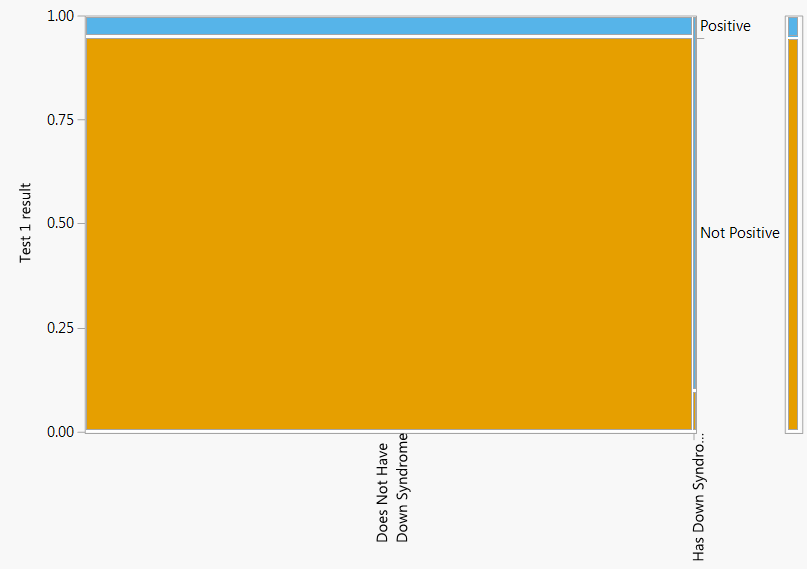
\includegraphics[width=2.69in,height=\textheight,keepaspectratio]{_graphics/DS-mosaic2.png}

}

\subcaption{\label{fig-DS-mosaic-twoway-1}Conditioning on DiGeorge
Syndrome status.}

\end{minipage}%
%
\begin{minipage}{0.50\linewidth}

\centering{

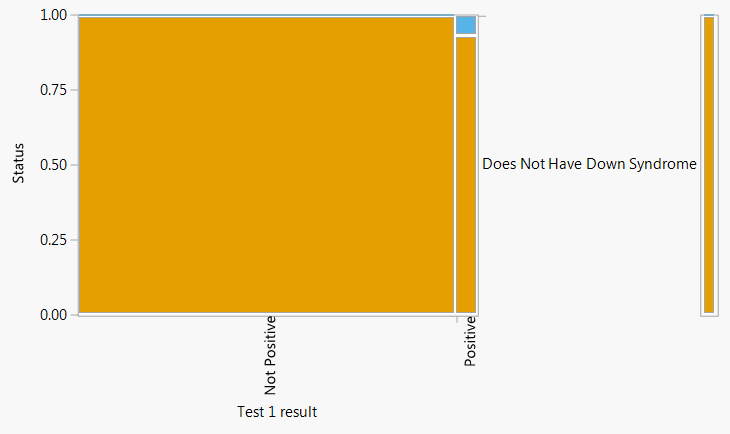
\includegraphics[width=2.43in,height=\textheight,keepaspectratio]{_graphics/DS-mosaic.png}

}

\subcaption{\label{fig-DS-mosaic-twoway-2}Conditioning on test result.}

\end{minipage}%

\caption{\label{fig-DS-mosaic-twoway}Mosaic plots for
Example~\ref{exm-bayes-false-positive-twoway}.}

\end{figure}%

People have a tendency to ignore base rates; you probably did if your
original guess in Example~\ref{exm-bayes-false-positive-twoway} was 0.7
or 0.9. Don't neglect the base rates when evaluating probabilities! We
will discuss the role that base rates play and how to revise
probabilities in light of new information in much more detail later.

We close this section with a brief tangent relating to the discussion in
Section~\ref{sec-which-interpretation}. In
Example~\ref{exm-bayes-false-positive-twoway} there is uncertainty due
to the random selection, uncertainty about whether the test will be
positive or not, and uncertainty that someone who tests positive
actually has the condition. You might consider these three different
kinds of randomness, with three different interpretations of
corresponding probabilities. For example, you might interpret the
probability that a randomly selected person has the condition (0.00025)
as a long run relative frequency; however, once the person is selected
and tests positive they either have the condition or not---we just don't
know for sure---so you might interpret the probability that they have
the condition given a positive test (0.0797) differently. The point is:
how we interpret the probabilities does not affect how we solve the
problem. The probabilities involved in
Example~\ref{exm-bayes-false-positive-twoway} ``fit together'' in the
same way regardless of the interpretation; given the context and values
0.00025, 0.9, and 0.0026 we must arrive at 0.0797. Furthermore, to make
sense of the value 0.0797 we used both long run relative frequency and
relative degrees of likelihood interpretations. We will treat many
examples like Example~\ref{exm-bayes-false-positive-twoway}; we will
generally not distinguish between different types of randomness, and we
will use interpretations of probability interchangeably.

\subsection{Exercises}\label{exercises-3}

\begin{exercise}[]\protect\hypertarget{exr-greater-prob-of-what}{}\label{exr-greater-prob-of-what}

In each of the following, which is greater: (a) or (b)? Or are they
equal? Or is there not enough information to decide?

\begin{enumerate}
\def\labelenumi{\arabic{enumi}.}
\tightlist
\item
  Surfing

  \begin{enumerate}
  \def\labelenumii{\alph{enumii}.}
  \tightlist
  \item
    The probability that a randomly selected Californian likes to surf.
  \item
    The probability that a randomly selected American is a Californian
    who likes to surf
  \end{enumerate}
\item
  Cal Poly alums

  \begin{enumerate}
  \def\labelenumii{\alph{enumii}.}
  \tightlist
  \item
    The probability that a California resident is a Cal Poly alum.
  \item
    The probability that a Cal Poly alum is a California resident
  \end{enumerate}
\end{enumerate}

\end{exercise}

\begin{exercise}[]\protect\hypertarget{exr-more-cats-dogs}{}\label{exr-more-cats-dogs}

Continuing Example~\ref{exm-cats-dogs}.

\begin{enumerate}
\def\labelenumi{\arabic{enumi}.}
\tightlist
\item
  Is the overall percentage of American adults who have a pet cat closer
  to the value in part 9 or part 10? Why do you think that is?
\item
  What percentage of American adults who have a pet dog also have a pet
  cat?
\item
  What percentage of American adults who do not have a pet dog have a
  pet cat?
\end{enumerate}

\end{exercise}

\begin{exercise}[]\protect\hypertarget{exr-more-cats-dogs-2}{}\label{exr-more-cats-dogs-2}

Continuing Example~\ref{exm-cats-dogs}. Now suppose that 11.75\% of
American adults have both a pet cat and a pet dog (as Donny claimed was
necessarily true). Redo Example~\ref{exm-cats-dogs} and
Exercise~\ref{exr-more-cats-dogs} under this assumption. What is true in
this scenario that wasn't true in Example~\ref{exm-cats-dogs}?

\end{exercise}

\begin{exercise}[]\protect\hypertarget{exr-grad-school-two-way}{}\label{exr-grad-school-two-way}

Suppose that you have applied to two graduate schools, A and B. Your
subjective probability of being accepted is 0.6 for school A and 0.7 for
school B.

\begin{enumerate}
\def\labelenumi{\arabic{enumi}.}
\tightlist
\item
  What is the largest possible probability of being accepted by both
  schools? Under what scenario (however unrealistic) would this be true?
  Explain.
\item
  What is the smallest possible probability of being accepted by both
  schools? Under what scenario (however unrealistic) would this be true?
  Explain.
\item
  Explain why the probability of being accepted by both schools is not
  necessarily 0.42.
\item
  For the remaining parts, suppose your subjective probability of being
  accepted at both schools is 0.55. If you are accepted at school A,
  what is your probability of also being accepted at school B?
\item
  If you are accepted at school A, what is your probability of not being
  accepted at school B?
\item
  If you are not accepted at school A, what is your probability of being
  accepted at school B?
\item
  If you are accepted at school B, what is your probability of also
  being accepted at school A?
\item
  If you are not accepted at school B, what is your probability of being
  accepted at school A?
\item
  How much more likely are you to be accepted at school A if you are
  accepted at school B than if you are not accepted at school B?
\item
  How much more likely are you to be accepted at school A if you are
  accepted at school B compared to before receiving the decision from
  school B?
\end{enumerate}

\end{exercise}

\section{Conditioning on information}\label{sec-literacy-conditioning}

A probability is a measure of the likelihood or degree of uncertainty or
plausibility of an event. A ``conditional'' probability revises this
measure to reflect any additional information about the outcome of the
underlying random phenomenon. In
Example~\ref{exm-bayes-false-positive-twoway} the probability that a
baby has DiGeorge syndrome is 0.00025, but if the screening returns a
positive result then the probability increases to 0.0797. Always look
out for words like ``if'' or ``given'' which signify information that
influences probabilities.

\begin{tcolorbox}[enhanced jigsaw, opacityback=0, left=2mm, colframe=quarto-callout-note-color-frame, toprule=.15mm, breakable, colback=white, leftrule=.75mm, arc=.35mm, rightrule=.15mm, bottomrule=.15mm]

\begin{example}[]\protect\hypertarget{exm-probability-interpret-conditional}{}\label{exm-probability-interpret-conditional}

In each of the following parts, which of the two probabilities, (a) or
(b), is greater, or are they equal? You should answer conceptually
without attempting any calculations.

\begin{enumerate}
\def\labelenumi{\arabic{enumi}.}
\item
  Imagine that you randomly select, from birth records, a person who was
  born in 1950.

  \begin{enumerate}
  \def\labelenumii{\alph{enumii}.}
  \tightlist
  \item
    The probability that a person born in 1950 lives to age 100.
  \item
    The probability that a person born in 1950 lives to age 100 given
    that they are alive in 2045.
  \end{enumerate}
\item
  Imagine the 2032 U.S. Presidential Election (we're doing so as of this
  writing in 2023). Assume (a) and (b) below are not 0.

  \begin{enumerate}
  \def\labelenumii{\alph{enumii}.}
  \tightlist
  \item
    The probability that Dwayne ``The Rock'' Johnson wins the 2032 U.S.
    Presidential Election.
  \item
    The probability that Dwayne ``The Rock'' Johnson wins the 2032 U.S.
    Presidential Election given that he does not win the nomination of
    the Democratic or the Republican Party.
  \end{enumerate}
\end{enumerate}

\end{example}

\end{tcolorbox}

\begin{tcolorbox}[enhanced jigsaw, opacityback=0, rightrule=.15mm, coltitle=black, colframe=quarto-callout-tip-color-frame, toprule=.15mm, colbacktitle=quarto-callout-tip-color!10!white, opacitybacktitle=0.6, left=2mm, toptitle=1mm, breakable, title={Solution (click to expand)}, bottomtitle=1mm, colback=white, leftrule=.75mm, titlerule=0mm, arc=.35mm, bottomrule=.15mm]

\begin{refsolution}
\leavevmode

\begin{enumerate}
\def\labelenumi{\arabic{enumi}.}
\item
  The probability in (b) is greater. Someone who has already lived to
  age 95 has a better chance of living at least 5 more years than a
  person has of living from birth to age 100. Think in fraction terms.
  The denominator in (a) is all people born in 1950; the denominator in
  (b) is all people born in 1950 who are alive in 2045. It's the same
  numerator in each case---people born in 1950 who live until age
  100---but (b) has a much smaller denominator, so the fraction
  corresponding to (b) is larger.
\item
  This is more subjective, but our assessment is that the probability in
  (a) is greater. As of this writing (2023), the 2032 election is still
  many years away so there is a great deal of uncertainty about who will
  even run let alone win (to say nothing about uncertainty regarding
  changes in the U.S. and the world that might happen before 2032 and
  affect the election). Dwayne Johnson's name has been tossed around in
  the media as a potential presidential candidate, so let's say he has
  some non-zero probability of winning, represented by (a) (which could
  be very small). As of this writing, we would assess the probability of
  someone other than the Democratic or Republican nominee winning a U.S.
  presidential election to be very small, and some pretty major changes
  would need to occur in order for us to change that assessment. So the
  information that Dwayne Johnson is the nominee of neither party would
  lead us to decrease his probability of winning the election.
\end{enumerate}

\label{sol-probability-interpret-conditional}

\end{refsolution}

\end{tcolorbox}

In a sense, all probabilities are conditional upon some information,
even if that information is vague (``well, it has to be one of these
possibilities''). Be careful to clearly identify what information is
reflected in probabilities, and don't make assumptions. In part 1 of
Example~\ref{exm-probability-interpret-conditional} if we're randomly
selecting a person from 1950 birth records, then we shouldn't assume
that the person is alive today when evaluating the probability in (a);
the selected person could have died between 1950 and now. That is, ``the
probability that a person born in 1950 lives to age 100'' is not the
same as ``the probability that a person born in 1950 \emph{who is alive
today} lives to age 100''. In part 2 of
Example~\ref{exm-probability-interpret-conditional}, we shouldn't assume
that Dwayne Johnson actually runs for president in 2032; the value of
our probability should reflect that uncertainty. That is, ``the
probability that Dwayne Johnson wins the 2032 U.S. Presidential
Election'' is not the same as ``the probability that Dwayne Johnson wins
the 2032 U.S. Presidential Election \emph{given that he declares himself
a candidate}''.

\begin{tcolorbox}[enhanced jigsaw, opacityback=0, left=2mm, colframe=quarto-callout-note-color-frame, toprule=.15mm, breakable, colback=white, leftrule=.75mm, arc=.35mm, rightrule=.15mm, bottomrule=.15mm]

\begin{example}[]\protect\hypertarget{exm-harry-second}{}\label{exm-harry-second}

Consider a group of 5 people: Harry, Fleur, Viktor, Cedric, Angelina.
Suppose each of their names is written on a slip of paper and the 5
slips of paper are placed into a hat. The papers are mixed up and 2 are
pulled out, one after the other \emph{without} replacement. (That is,
the first paper is not added back to the hat before selecting the
second.)

\begin{enumerate}
\def\labelenumi{\arabic{enumi}.}
\tightlist
\item
  What is the probability that Harry is the first name selected?
\item
  What is the probability that Harry is the second name selected?
\item
  If you were asked question (2) before question (1), would your answer
  change? Should it?
\item
  If Fleur is the first name selected, what is the probability that
  Harry is the second name selected?
\item
  If Harry is not the first name selected, what is the probability that
  Harry is the second name selected?
\item
  If Harry is the first name selected, what is the probability that
  Harry is the second name selected?
\item
  Construct a hypothetical table corresponding to the results of the
  draws. Hint: one dimension represents the result of the first draw
  which is Harry or not, and the other dimension represents the second
  draw.
\item
  If Fleur is the second name selected, what is the probability that
  Harry was the first name selected?
\end{enumerate}

\end{example}

\end{tcolorbox}

\begin{tcolorbox}[enhanced jigsaw, opacityback=0, rightrule=.15mm, coltitle=black, colframe=quarto-callout-tip-color-frame, toprule=.15mm, colbacktitle=quarto-callout-tip-color!10!white, opacitybacktitle=0.6, left=2mm, toptitle=1mm, breakable, title={Solution (click to expand)}, bottomtitle=1mm, colback=white, leftrule=.75mm, titlerule=0mm, arc=.35mm, bottomrule=.15mm]

\begin{refsolution}
\leavevmode

\begin{enumerate}
\def\labelenumi{\arabic{enumi}.}
\item
  The probability that Harry is the first name selected is 1/5, which is
  an answer we think most people would agree with. There are 5 names
  which are equally likely to be the first one selected, 1 of which is
  Harry.
\item
  The probability that Harry is the second name selected is also 1/5.
  Many people might answer this as 1/4, since after selecting the first
  person there are now 4 names left. But we show and discuss below that
  the \emph{unconditional} probability is 1/5.
\item
  Your answer to question (2) certainly shouldn't change depending on
  whether we ask question (1) first. But perhaps after seeing question
  (1) you are implicitly assuming that Harry has not been selected
  first? But there is nothing in question (2) that gives you any
  additional \emph{information} about what happened on the first card.
\item
  If Fleur is the first name selected, the probability that Harry is the
  second name selected is 1/4. We think most people find this intuitive.
  If Fleur is first, there are 4 cards remaining, equally likely to be
  the next card, of which 1 is Harry.
\item
  1/4, similar to the previous part. If Harry is not selected first,
  there are 4 cards remaining, equally likely to be the next card, of
  which 1 is Harry.
\item
  If Harry is the first name selected, the probability that Harry is the
  second name selected is 0 since the cards are drawn \emph{without}
  replacement.
\item
  Here is a two-way table of 1000 hypothetical repetitions. Harry is
  selected first in \(1000\times 1/5 = 200\) repetitions, in which case
  he can't be selected second. Among the 800 repetitions where Harry is
  not selected first, he is selected second in \(800\times 1/4 = 200\)
  repetitions. Harry is selected second in 200 of the 1000 total
  repetitions, so the probability that Harry is selected second is
  \(200/1000 = 1/5\).

  \begin{longtable}[]{@{}lrrr@{}}
  \toprule\noalign{}
  & Harry first & Harry not first & Total \\
  \midrule\noalign{}
  \endhead
  \bottomrule\noalign{}
  \endlastfoot
  Harry second & 0 & 200 & 200 \\
  Harry not second & 200 & 600 & 800 \\
  Total & 200 & 800 & 1000 \\
  \end{longtable}
\item
  If Fleur is the second name selected, the probability that Harry was
  the first name selected is 1/4. It doesn't really matter what is
  ``first'' and what is ``second'', but rather the information conveyed.
  In part 4, what's important is that you know that one of the cards
  selected was Fleur, so the probability that the other card selected is
  Harry is 1/4. But this part conveys the same information.
\end{enumerate}

\label{sol-harry-second}

\end{refsolution}

\end{tcolorbox}

\textbf{Be careful to distinguish between conditional and unconditional
probabilities.} A conditional probability reflects additional
information about the outcome of the random phenomenon. In the absence
of such information, we must continue to account for all the
possibilities. When computing probabilities, be sure to only reflect
information that is known. Especially when considering a phenomenon that
happens in stages, don't assume that when considering what happens
second that you know what happened first.

In Example~\ref{exm-harry-second}, the question ``if Harry is not the
first name selected, what is the probability that Harry is the second
name selected?'' involves a \emph{conditional} probability, since we are
given additional information about the outcome; it is no longer possible
that Harry was the first name selected. The question ``What is the
probability that Harry is the second name selected?'' involves an
\emph{unconditional} probability. The words ``the probability that Harry
is the second name selected'' alone do not imply that Harry was not
selected first; we still need to account for the possibility that Harry
was selected first.

Imagine shuffling the five cards and putting two on a table face down.
Now point to one of the cards and ask ``what is the probability that
THIS card is Harry?'' Well, all you know is that this card is one of the
five cards, each of the 5 cards is equally likely to be the one you're
pointing to, and only one of the cards is Harry. Should it matter
whether the face down card you're pointing to was the first or second
card you laid on the table? No, the probability that THIS card is Harry
should be 1/5, regardless of whether you put it down first or second.

Now turn over one other card that you're not pointing to, and see what
name is on it. The probability that the card you're pointing to is Harry
has now changed, because you have some information about the outcome of
the shuffle. If the card you turned over says Harry, you know the
probability that the card you're pointing to is Harry is 0. If the card
you turned over is not Harry, then you know that the probability that
the card you're pointing to is Harry is 1/4. It is not ``first'' or
``second'' that matters; it is whether or not you have obtained
additional information by revealing one of the cards.

Another way of asking the question is: Shuffle the five cards; what is
the probability that Harry is the second card from the top? Without
knowing any information about the result of the shuffle, all you know is
that Harry should be equally likely to be in any one of the 5 positions,
so the probability that he is the second card from the top should be
1/5. It is only after revealing information about the result of the
shuffle, say the top card, that the probability that Harry is in the
second position changes.

We often start with a probability for an event and then revise it
whenever additional information becomes available. The original,
unconditional probability is called a ``prior probability'' or ``base
rate''; the revised, conditional probability is called a ``posterior
probability''. We will discuss the role that base rates play and how to
revise probabilities in light of additional information in much more
detail later. But remember: Don't neglect the base rates when evaluating
probabilities!

\begin{tcolorbox}[enhanced jigsaw, opacityback=0, left=2mm, colframe=quarto-callout-note-color-frame, toprule=.15mm, breakable, colback=white, leftrule=.75mm, arc=.35mm, rightrule=.15mm, bottomrule=.15mm]

\begin{example}[]\protect\hypertarget{exm-base-rate-neglect}{}\label{exm-base-rate-neglect}

Within both the colleges of Agriculture and Architecture at Cal Poly,
about 49\% of admitted students are female, about 84\% of admitted
students went to high school in CA, and the median GPA of admitted
students is about 4.1.

An orientation group of 100 newly admitted Cal Poly students includes 75
students in Agriculture and 25 students in Architecture. A student is
randomly selected from this group. The selected student is Maddie, who
is female, went to high school in CA, and had a high school GPA of 4.1.

\begin{enumerate}
\def\labelenumi{\arabic{enumi}.}
\tightlist
\item
  If you are trying to decide which college Maddie is in, is the
  information that she is female, went to high school in CA, and had a
  high school GPA of 4.1 helpful? Why?
\item
  Donny Don't says, ``The information about Maddie applies equally well
  to Agriculture or Architecture and doesn't help us decide which
  college she's in, so it's just 50/50. Given the information about
  Maddie, the conditional probability that she is in Agriculture is
  0.5.'' Do you agree? If not, what is the conditional probability that
  Maddie is in the college of Agriculture given the information about
  her? Hint: what was the last sentence before this example!
\end{enumerate}

\end{example}

\end{tcolorbox}

\begin{tcolorbox}[enhanced jigsaw, opacityback=0, rightrule=.15mm, coltitle=black, colframe=quarto-callout-tip-color-frame, toprule=.15mm, colbacktitle=quarto-callout-tip-color!10!white, opacitybacktitle=0.6, left=2mm, toptitle=1mm, breakable, title={Solution (click to expand)}, bottomtitle=1mm, colback=white, leftrule=.75mm, titlerule=0mm, arc=.35mm, bottomrule=.15mm]

\begin{refsolution}
\leavevmode

\begin{enumerate}
\def\labelenumi{\arabic{enumi}.}
\tightlist
\item
  The information tells us that Maddie would be pretty typical for
  either group, so it doesn't help us decide.
\item
  Donny has neglected the base rate. The group has 75 students in
  Agriculture and 25 students in Architecture. If we randomly select a
  student from this group, the unconditional probability that the
  selected student is in Agriculture is 0.75 (the base rate). Yes, the
  information about Maddie applies equally well to either college, but
  that means we have no reason to revise our probability from the base
  rate. The conditional probability that Maddie is in Agriculture given
  the information about her is still 0.75.
\end{enumerate}

\label{sol-bayes-false-positive-twoway}

\end{refsolution}

\end{tcolorbox}

We use the terminology ``unconditional'' and ``conditional''
probability, but any probability is conditional on some information. A
better way to think about it might just be ``before'' and ``after''.
When new information becomes available we revise our probability. The
unconditional (prior) probability is the probability before the
revision, reflecting any information that was previously available. The
conditional (posterior) probability is the probability after the
revision, updated to reflect the newly available information.
Probabilities are often updated sequentially as more information becomes
available, with the conditional (posterior) probability after one piece
of information is received becoming the unconditional (prior)
probability before the next.

Do not think of ``unconditional'' as ``based on no information''. Any
probability should reflect as much relevant information as possible,
even if it plays the role of an unconditional probability.

\begin{tcolorbox}[enhanced jigsaw, opacityback=0, left=2mm, colframe=quarto-callout-note-color-frame, toprule=.15mm, breakable, colback=white, leftrule=.75mm, arc=.35mm, rightrule=.15mm, bottomrule=.15mm]

\begin{example}[]\protect\hypertarget{exm-base-rate-pregnancy}{}\label{exm-base-rate-pregnancy}

Marge takes a home pregnancy test which turns out positive. She decides
to perform an analysis like in
Example~\ref{exm-bayes-false-positive-twoway} to find the conditional
probability that she is actually pregnant given the positive test. She
knows she'll need a base rate---that is, an unconditional probability
that she is pregnant before the positive test---so she Googles ``what
percent of women are pregnant?''
\href{https://www.cdc.gov/nchs/products/databriefs/db136.htm}{Information
from the CDC} suggests that 10.2\% of American women aged 15--44 are
pregnant at any point in time. Is 0.102 an appropriate value for Marge
to use as her base rate? Or is it too high or too low? How will this
influence her conditional probability that she is actually pregnant
given the positive test? Explain. Hint: did Marge Google the right
question?

\end{example}

\end{tcolorbox}

\begin{tcolorbox}[enhanced jigsaw, opacityback=0, rightrule=.15mm, coltitle=black, colframe=quarto-callout-tip-color-frame, toprule=.15mm, colbacktitle=quarto-callout-tip-color!10!white, opacitybacktitle=0.6, left=2mm, toptitle=1mm, breakable, title={Solution (click to expand)}, bottomtitle=1mm, colback=white, leftrule=.75mm, titlerule=0mm, arc=.35mm, bottomrule=.15mm]

\begin{refsolution}
The value 0.102 is too low for Marge to use as a base rate, and so her
conditional probability that she is actually pregnant given the positive
test will also be too low. The idea is that a woman \emph{who takes a
pregnancy test} is more likely to be pregnant than a woman in general,
simply because many women who take pregnancy tests do so because they
suspect they might be pregnant\footnotemark{}.

If we randomly select an American woman aged 15-44 to take a pregnancy
test, then 0.102 would be an appropriate base rate. But we are not told
that Marge is a randomly selected woman, so we should not assume that
she is. What we do know is that ``Marge took a pregnancy test''. Why?
From our perspective, it seems more plausible that she took the test
because she suspected she might be pregnant as opposed to just
``randomly'' deciding to take it. And if there is a reason for her to
suspect she might be pregnant, then it's more likely that she actually
is and our base rate should reflect that, resulting in a value greater
than 0.102. It should be even clearer from Marge's perspective; she
knows why she took the test (e.g., missed period, morning sickness,
etc.) and her personal base rate should reflect her information.

Now we're not saying it would be easy to determine what an appropriate
base rate is, but it should definitely be greater than 0.102. Whatever
the prior probability of pregnancy, it will influence the posterior
probability of pregnancy given a positive test. Knowing that the test is
positive will lead us to revise our probability of pregnancy upward, but
if we start with a prior probability that is too low, then our posterior
probability will also be too low. (See the last part of
Example~\ref{exm-bayes-false-positive-twoway} for a related example.)

\label{sol-base-rate-pregnancy}

\end{refsolution}

\end{tcolorbox}

\footnotetext{Pregnancy tests are included as part of health screenings
for other reasons, but most women who take home pregnancy tests do so
for pregnancy related reasons.}

\subsection{Exercises}\label{exercises-4}

\begin{exercise}[]\protect\hypertarget{exr-greater-conditioning-literacy}{}\label{exr-greater-conditioning-literacy}

In each of the following, which is greater: (a) or (b)? Or are they
equal? Or is there not enough information to decide? Answer without
doing any computations.

\begin{enumerate}
\def\labelenumi{\arabic{enumi}.}
\tightlist
\item
  Shuffle a standard deck of playing cards (52 cards, 4 of which are
  aces) and deal 5 cards without replacement.

  \begin{enumerate}
  \def\labelenumii{\alph{enumii}.}
  \tightlist
  \item
    The probability that the first card dealt is an ace.
  \item
    The probability that the firth card dealt is an ace.
  \end{enumerate}
\item
  Shuffle a standard deck of playing cards (52 cards, 4 of which are
  aces) and deal 5 cards without replacement.

  \begin{enumerate}
  \def\labelenumii{\alph{enumii}.}
  \tightlist
  \item
    The probability that the first card dealt is an ace.
  \item
    The probability that the fifth card dealt is an ace if the first
    card dealt is an ace.
  \end{enumerate}
\item
  Randomly select a college student.

  \begin{enumerate}
  \def\labelenumii{\alph{enumii}.}
  \tightlist
  \item
    The probability that the selected student went surfing yesterday.
  \item
    The probability that the selected student went surfing yesterday if
    they student attends Cal Poly.
  \end{enumerate}
\item
  Both ballerinas and football players are graceful and nimble. A group
  of people contains both some ballerinas and some football players. A
  person is randomly selected from this group; the person is graceful
  and nimble.

  \begin{enumerate}
  \def\labelenumii{\alph{enumii}.}
  \tightlist
  \item
    The probability that the selected person is a ballerina.
  \item
    The probability that the selected person is a football player.
  \end{enumerate}
\end{enumerate}

\end{exercise}

\section{Probability of what?}\label{sec-probofwhat}

A probability takes a value in the sliding scale from 0 to 1 (or 0\% to
100\%). Throughout the book we will study how to compute probabilities
in many situations. But don't just focus on computation. Always remember
to interpret probabilities properly. This section covers a few ideas to
keep in mind when interpreting probabilities.

\begin{tcolorbox}[enhanced jigsaw, opacityback=0, left=2mm, colframe=quarto-callout-note-color-frame, toprule=.15mm, breakable, colback=white, leftrule=.75mm, arc=.35mm, rightrule=.15mm, bottomrule=.15mm]

\begin{example}[]\protect\hypertarget{exm-probability-interpret1}{}\label{exm-probability-interpret1}

In each of the following parts, which of the two probabilities, a or b,
is greater, or are they equal? You should answer conceptually without
attempting any calculations.

\begin{enumerate}
\def\labelenumi{\arabic{enumi}.}
\item
  Flip a coin \emph{which is known to be fair} 10 times.

  \begin{enumerate}
  \def\labelenumii{\alph{enumii}.}
  \tightlist
  \item
    The probability that the results are, in order, HHHHHHHHHH.
  \item
    The probability that the results are, in order, HHTHTTTHHT.
  \end{enumerate}
\item
  Flip a coin which is known to be fair 10 times.

  \begin{enumerate}
  \def\labelenumii{\alph{enumii}.}
  \tightlist
  \item
    The probability that all 10 flips land on H.
  \item
    The probability that exactly 5 flips land on H.
  \end{enumerate}
\end{enumerate}

\end{example}

\end{tcolorbox}

\begin{tcolorbox}[enhanced jigsaw, opacityback=0, rightrule=.15mm, coltitle=black, colframe=quarto-callout-tip-color-frame, toprule=.15mm, colbacktitle=quarto-callout-tip-color!10!white, opacitybacktitle=0.6, left=2mm, toptitle=1mm, breakable, title={Solution (click to expand)}, bottomtitle=1mm, colback=white, leftrule=.75mm, titlerule=0mm, arc=.35mm, bottomrule=.15mm]

\begin{refsolution}
\leavevmode

\begin{enumerate}
\def\labelenumi{\arabic{enumi}.}
\item
  Many people would say the probability in (b) is larger, but the
  probabilities in (a) and (b) are equal\footnotemark{}. The sequence in
  (b) seems to look ``more random''. However, the probability of seeing
  that particular sequence---H then H then T then H then T\ldots---is
  the same as seeing the sequence H then H then H then H then H\ldots{}
  If the coin is fair and the flips are independent, all possible
  sequences of flips are equally likely. Think of it this way: choose
  any flip, say the third. Then that flip is equally likely to be H (as
  in the third flip for (a)) or T (as in the third flip for (b)). No
  matter which flip it is, or the results of the other flips, any flip
  is equally likely to be H or T.

  Of course, our response assumes that the coin is fair. If the coin is
  known to be fair then the sequences in (a) and (b) are equally likely.
  However, if we actually observed the sequence in (a) we might suspect
  that the coin is actually not fair. There is an important difference
  between assumption and observation.
\item
  The probability in (b) is larger. Contrast this to the previous part.
  There is only one sequence which results in 10 heads, HHHHHHHHHH.
  However, there are many sequences\footnotemark{} which result in
  exactly 5 heads---HHHHHTTTTT, HTHTHTHTHT, TTHHTHTHHT, etc---of which
  HHTHTTTHHT is just one possibility.
\end{enumerate}

\label{sol-probability-interpret1}

\end{refsolution}

\end{tcolorbox}

\footnotetext{And both equal to
\(\left(\frac{1}{2}\right)^{10} =\frac{1}{1024}\)}

\footnotetext{252 out of 1024 possibilities in fact}

Pay close attention to the differences in the two parts in
Example~\ref{exm-probability-interpret1}. The first part involves
probabilities of the particular outcome sequence. The second part
involves more general ``events'' that the particular outcome sequence
might satisfy. The following provides another example of this
``particular'' versus ``general'' dichotomy.

\begin{tcolorbox}[enhanced jigsaw, opacityback=0, left=2mm, colframe=quarto-callout-note-color-frame, toprule=.15mm, breakable, colback=white, leftrule=.75mm, arc=.35mm, rightrule=.15mm, bottomrule=.15mm]

\begin{example}[]\protect\hypertarget{exm-probability-interpret2}{}\label{exm-probability-interpret2}

In each of the following parts, which of the two probabilities, a or b,
is greater, or are they equal? You should answer conceptually without
attempting any calculations.

\begin{enumerate}
\def\labelenumi{\arabic{enumi}.}
\item
  In the \href{https://www.powerball.com/}{Powerball lottery} there are
  roughly\footnotemark{} 300 million possible winning number
  combinations, all equally likely.

  \begin{enumerate}
  \def\labelenumii{\alph{enumii}.}
  \tightlist
  \item
    The probability you win the next Powerball lottery if you purchase a
    single ticket, 4-8-15-16-42, plus the Powerball number, 23.
  \item
    The probability you win the next Powerball lottery if you purchase a
    single ticket, 1-2-3-4-5, plus the Powerball number, 6.
  \end{enumerate}
\item
  Continuing with the Powerball

  \begin{enumerate}
  \def\labelenumii{\alph{enumii}.}
  \tightlist
  \item
    The probability that the numbers in the winning number are in a row.
  \item
    The probability that the numbers in the winning number are not in a
    row.
  \end{enumerate}
\end{enumerate}

\end{example}

\end{tcolorbox}

\footnotetext{The exact count is 292,201,338. We will see how to compute
this number later.}

\begin{tcolorbox}[enhanced jigsaw, opacityback=0, rightrule=.15mm, coltitle=black, colframe=quarto-callout-tip-color-frame, toprule=.15mm, colbacktitle=quarto-callout-tip-color!10!white, opacitybacktitle=0.6, left=2mm, toptitle=1mm, breakable, title={Solution (click to expand)}, bottomtitle=1mm, colback=white, leftrule=.75mm, titlerule=0mm, arc=.35mm, bottomrule=.15mm]

\begin{refsolution}
\leavevmode

\begin{enumerate}
\def\labelenumi{\arabic{enumi}.}
\tightlist
\item
  Many people would say the probability in (a) is larger, since the
  sequence in (a) looks ``more random'', but the probabilities in (a)
  and (b) are equal. Since the outcomes are equally likely, the
  probability that any single sequence is the winning number is
  (roughly) 1/300,000,000. If you don't believe this, ask yourself: Why
  would the Powerball conduct its drawing in such a way that some
  numbers are more likely to be winners than others? And if some numbers
  were more likely than others, why wouldn't people know about this?
\item
  The probability in (b) is larger. Contrast this to the previous part.
  There are only a handful of winning numbers for which the numbers are
  in a row: 1 through 6, 2 through 7, 3 through 8, etc. However, almost
  all of the 300 million possibilities do not have numbers in a row.
\end{enumerate}

\label{sol-probability-interpret2}

\end{refsolution}

\end{tcolorbox}

When interpreting probabilities, be careful not to confuse ``the
particular'' with ``the general''.

\textbf{``The particular:''} A very specific event, surprising or not,
often has low probability.

\begin{itemize}
\tightlist
\item
  For a fair coin, observing the particular sequence HHTHTTTHHT in 10
  flips is just as likely as observing HHHHHHHHHH.
\item
  The probability that the winning powerball number is 4-8-15-16-42-(23)
  is exactly the same as the probability that the winning powerball
  number is 1-2-3-4-5-(6).\\
\item
  The probability that you get a text from your best friend at 7:43pm
  two weeks from today inviting you to dinner at your favorite pizza
  place after you've just ordered pizza from there is probably pretty
  small. None of these items --- getting a text, having a friend invite
  you to dinner, ordering pizza from your favorite pizza place --- is
  unusual, but the chances of them all combining in this way at this
  particular time are fairly small.
\end{itemize}

\textbf{``The general:''} While a very specific event often has low
probability, if there are many like events their combined probability
can be high.

\begin{itemize}
\tightlist
\item
  There are many possible sequences of 10 coin flips which result in 5
  heads.
\item
  For almost all of the possible Poweball combinations the numbers are
  not in order.
\item
  The probability that some time in the next month or so a friend texts
  a dinner invitation is probably fairly high.
\end{itemize}

\begin{tcolorbox}[enhanced jigsaw, opacityback=0, left=2mm, colframe=quarto-callout-note-color-frame, toprule=.15mm, breakable, colback=white, leftrule=.75mm, arc=.35mm, rightrule=.15mm, bottomrule=.15mm]

\begin{example}[]\protect\hypertarget{exm-probability-interpret3}{}\label{exm-probability-interpret3}

Which of the following two probabilities is greater, or are they equal?
You should answer conceptually without attempting any calculations.

\begin{enumerate}
\def\labelenumi{\arabic{enumi}.}
\tightlist
\item
  The probability that you win the next Powerball lottery if you
  purchase a single ticket.
\item
  The probability that someone wins the next Powerball lottery. (FYI:
  especially when the jackpot is large, there are hundreds of millions
  of tickets sold.)
\end{enumerate}

\end{example}

\end{tcolorbox}

\begin{tcolorbox}[enhanced jigsaw, opacityback=0, rightrule=.15mm, coltitle=black, colframe=quarto-callout-tip-color-frame, toprule=.15mm, colbacktitle=quarto-callout-tip-color!10!white, opacitybacktitle=0.6, left=2mm, toptitle=1mm, breakable, title={Solution (click to expand)}, bottomtitle=1mm, colback=white, leftrule=.75mm, titlerule=0mm, arc=.35mm, bottomrule=.15mm]

\begin{refsolution}
The probability in (2) is \emph{much} greater. (This is an
understatement.)

\begin{itemize}
\tightlist
\item
  The probability that a specific powerball ticket is the winning number
  is about 1 in 300 million. So if you buy a single ticket, it is
  extremely unlikely that \emph{you} will win.
\item
  However, if hundreds of millions of powerball tickets are sold, the
  probability that \emph{someone somewhere} wins is pretty high.
\end{itemize}

We elaborate on these ideas below.

\label{sol-probability-interpret3}

\end{refsolution}

\end{tcolorbox}

The probability that you win the next Powerball lottery if you purchase
a single ticket is about 1 in 300 million. Let's put this number in
perspective. There are about 260 million adults (over age 18) in the
U.S.\footnote{Source:
  \href{https://www.census.gov/data/tables/2020/demo/popest/2020-demographic-analysis-tables.html}{U.S.
  Census Bureau}.} Suppose that the name of every adult in the U.S. is
written on a 3x5 index card. These 260 million cards stacked would
stretch about 62 miles high; that's commonly referenced as the
\href{https://astronomy.com/news/2021/03/the-krmn-line-where-does-space-begin}{distance
from the earth to where space begins}. The stack would also weigh about
400 tons, about as much 4 blue whales. Suppose we shuffle the
cards---much easier said than done---and select one. The probability
that your name is on the selected card is about 1 in 260 million. The
chances that your next Powerball ticket is the winning number are a
little less likely than this\footnote{The statistician
  \href{https://twitter.com/ron_wasserstein?lang=en}{Ron Wasserstein}
  has provided
  \href{https://www.huffpost.com/entry/chances-of-winning-powerball-lottery_b_3288129}{several}
  \href{https://www.huffpost.com/entry/if-winning-the-powerball-_b_8961606}{fanciful}
  \href{https://www.npr.org/2016/01/12/462754290/powerball-you-cant-win-if-you-dont-play}{perspectives}
  on the likelihood of winning the Powerball lottery.}.

However, if hundreds of millions of Powerball tickets are sold, the
probability that \emph{someone somewhere} wins is pretty high. For
example, if 500 million tickets are sold then there is a roughly 80\%
chance that at least one ticket has the winning number (under
\href{https://fivethirtyeight.com/features/new-powerball-odds-could-give-america-its-first-billion-dollar-jackpot/}{certain
assumptions}).

\textbf{Even if an event has extremely small probability, given enough
repetitions of the random phenomenon, the probability that the event
occurs on \emph{at least one} of the repetitions is often
high}\footnote{For an interesting investigation of this idea check out
  the \href{https://pudding.cool/2020/04/infinite/}{Infinite Monkey
  Theorem Experiment} at the site \href{https://pudding.cool/}{The
  Pudding}.}.

Consider the headline of this news article from 2010:
\href{https://www.upi.com/Odd_News/2010/06/24/Man-mauled-by-bear-after-lightning-strike/22821277399823/}{``Man
mauled by bear after lightning strike''}. We certainly feel sorry for
this poor man, but just how unlikely is such an occurrence? Let's look a
little closer.

The headline seems to imply that the man got struck by lightning and
then, while he was trying to reach safety, a bear attacked. But the
mauling occurred \emph{four years after} the lightning strike. Getting
mauled by a bear and struck by lightning within one's lifetime is
certainly much more likely than both happening on the same day.

``Getting struck by lightning'' is often colloquially used to describe a
rare event, but how unlikely is it? One
\href{https://www.vaisala.com/sites/default/files/documents/Annual_rates_of_lightning_fatalities_by_country.pdf}{study
estimates that about 250,000 people in the world are struck by lightning
each year}, and the
\href{https://www.weather.gov/safety/lightning-odds}{National Weather
Service} estimates that the probability that you get struck by lightning
within your lifetime is 1/15,000. Still not very likely, but maybe not
as rare as you might think.

Getting mauled by a bear is much less likely than being struck by
lightning. There are only
\href{https://www.nature.com/articles/s41598-019-44341-w}{about 40 bear
attacks of humans each year}. However, if the headline had been ``Man
bitten by shark after lightning strike'' or ``Man attacked by mountain
lion after lightning strike'' or ``Man trampled by moose after lightning
strike'' it probably would have been equally newsworthy. Thus we should
account for all similar animal attacks, not just bear attacks, when
assessing the likelihood.

The probability that you get struck by lightning and mauled by a bear
today is certainly very small. But the probability that someone
somewhere within their lifetime gets both struck by lightning and
attacked by an animal is orders of magnitude higher. In general, even
though the probability that something very specific happens to you today
is often extremely small, the probability that something similar happens
to someone some time is often quite high.

When something surprising happens, don't just consider the probability
of that particular outcome. Rather, consider all the other possible
outcomes that would have been equally surprising if they had occurred,
and consider the probability that at least one of them would happen
(which often turns out to be not so small). From this perspective, most
coincidences turn out to be much more probable than they seem at first.

When assessing a probability, always ask ``probability of what''? Does
the probability represent ``the particular'' or ``the general''? Is it
the probability that the event happens in a single occurrence of the
random phenomenon, or the probability that the event happens at least
once in many occurrences? Keep these questions in mind when assessing
numerical probabilities. Remember that something that has a ``one in a
million chance'' of happening to you today will happen to about 7000
people in the world every day.

\subsection{How likely is ``likely''?}\label{how-likely-is-likely}

Consider each of the following statements (presented in no particular
order). If you were to assign a numerical value to the probability of
rain tomorrow in each case, what would it be?

\begin{itemize}
\tightlist
\item
  It is likely that it will rain tomorrow.
\item
  It is probable that it will rain tomorrow.
\item
  There is little chance that it will rain tomorrow.
\item
  It is highly unlikely that it will rain tomorrow.
\item
  We doubt that it will rain tomorrow.
\item
  There is a very good chance that it will rain tomorrow.
\item
  It is almost certain that it will rain tomorrow.
\item
  It is improbable that it will rain tomorrow.
\item
  It will probably not rain tomorrow.
\item
  It is highly likely that it will rain tomorrow.
\item
  It is almost certain that it will not rain tomorrow.
\item
  It will probably rain tomorrow.
\item
  We believe that it will rain tomorrow.
\item
  There is a better than even chance that it will rain tomorrow.
\end{itemize}

In a study conducted in the 1960s (Barclay et al. (1977)), twenty-three
military officers were asked to provide numerical probabilities for a
similar set of statements (``It is almost certain that the Soviets will
invade Czechoslovakia'', ``It is highly likely that the Soviets will
invade Czechoslovakia'', etc.) For most of the statements there was
considerable variability in the responses. For example,

\begin{itemize}
\tightlist
\item
  Probabilities assigned to ``almost certain'' ranged from 0.75 to 0.99.
\item
  Probabilities assigned to ``highly likely'' ranged from 0.50 to 0.99.
\item
  Probabilities assigned to ``likely'' ranged from 0.30 to 0.90.
\item
  Probabilities assigned to ``probable'' ranged from 0.25 to 0.90.
\end{itemize}

Recent
\href{https://mirkomazzoleni.github.io/blog/2016/12/17/perception_of_probability/}{similar}
\href{https://waf.cs.illinois.edu/visualizations/Perception-of-Probability-Words/}{studies}
have produced comparable results that exhibit wide variability in the
numerical values people associate with words describing probabilities.
Studies like these provide evidence of differences in how people
perceive probability.

One way to avoid ambiguity is to provide numerical values of probability
rather than just vague words like ``likely'' or ``probable''. However,
people can still perceive numbers differently. An event that has a
probability of 0.4 is four times more likely than an event with a
probability of 0.1, but how likely is either event? Depending on their
background, people might interpret a probability of 0.4 differently.
Someone familiar with baseball knows that 0.4 would be an extremely high
value for the probability that a particular batter successfully gets a
hit in at bat, while someone familiar with basketball knows that 0.4
would be extremely low value for the probability that a particular
player successfully scores on a free throw attempt. An audience that
routinely encounters probabilities close to 0 will perceive a
probability of 0.4 differently than one that commonly deals with
probabilities around 0.5. When reporting probabilities, it is helpful to
provide some benchmarks from a context more familiar to the audience to
provide a sense of scale\footnote{This idea was inspired by
  \href{https://fivethirtyeight.com/features/xkcd-randall-munroe-qanda-what-if/}{Randall
  Munroe}.}.

For example, for people from California you might provide benchmarks
based on
\href{https://en.wikipedia.org/wiki/List_of_counties_in_California}{county
populations}. If you randomly select a single California resident (about
39 million people) there is, roughly, a

\begin{itemize}
\tightlist
\item
  25\% chance they are from Los Angeles County (about 9.7 million
  people)
\item
  8\% chance they are from Orange County (about 3.2 million people)
\item
  0.7\% chance they are from San Luis Obispo County (about 300 thousand
  people)
\item
  0.1\% chance they are from Calaveras County (about 46 thousand people)
\end{itemize}

Providing a few values in this manner can help the audience gauge the
magnitude of a probability like 0.2 or 0.01\footnote{For probabilities
  closer to 1, we could report the chances of \emph{not} being from
  these counties.}.

Be sure to keep in mind ``the particular versus the general''. When
reporting the value of a probability, provide enough contextual detail
so that the audience can distinguish ``the particular from the
general''. If the probability of interest represents ``the particular'',
then provide benchmarks in terms of ``the particular''; likewise for
``the general''. In the California county example, we could use the
values provided for a \emph{single} randomly selected resident to
benchmark ``particular'' probabilities (what is the probability this
happens to me?). For ``general'' probabilities we could revise in terms
like ``if we randomly select 100 CA residents, there is a 50\% chance
that at least one resident is from San Luis Obispo County''.

So how likely is ``likely''? We hope you see that there is no clear
answer to this question. When communicating probabilities, our best
advice is to:

\begin{itemize}
\tightlist
\item
  Report numerical values instead of ambiguous words.
\item
  Provide enough contextual detail to identify ``probability of what?''.
  In particular, be careful to distinguish ``the particular from the
  general''.
\item
  Provide the value of a few helpful benchmark probabilities in a
  familiar context to provide a sense of scale.
\item
  Remember that despite your best efforts, people might still perceive
  probabilities differently.
\end{itemize}

\subsection{Exercises}\label{exercises-5}

\begin{exercise}[]\protect\hypertarget{exr-powerball-analogy}{}\label{exr-powerball-analogy}

Create your own analogy for how unlikely that a single ticket wins the
Powerball lottery. How would you describe a 1 in 300 million chance?

\end{exercise}

\begin{exercise}[]\protect\hypertarget{exr-greater-particular-vs-general}{}\label{exr-greater-particular-vs-general}

In each of the following, which is greater: (a) or (b)? Or are they
equal? Or is there not enough information to decide?

\begin{enumerate}
\def\labelenumi{\arabic{enumi}.}
\tightlist
\item
  Election interference

  \begin{enumerate}
  \def\labelenumii{\alph{enumii}.}
  \tightlist
  \item
    The probability that Russian agents successfully interfere with the
    2024 U.S. Presidential election through posts on Facebook with the
    goal of helping the Republican candidate get elected.
  \item
    The probability that non-U.S. actors attempt to interfere with the
    2024 U.S Presidential election.
  \end{enumerate}
\item
  Roll a six-sided die which is known to be fair 10 times.

  \begin{enumerate}
  \def\labelenumii{\alph{enumii}.}
  \tightlist
  \item
    The probability that the results are, in order, 1223334444.
  \item
    The probability that the results are, in order, 4614253226.
  \end{enumerate}
\item
  Roll a six-sided die which is known to be fair 10 times.

  \begin{enumerate}
  \def\labelenumii{\alph{enumii}.}
  \tightlist
  \item
    The probability that the results are, in order, 1234561234.
  \item
    The probability that you roll each of the six faces at least once.
  \end{enumerate}
\end{enumerate}

\end{exercise}

\begin{exercise}[]\protect\hypertarget{exr-benchmarks}{}\label{exr-benchmarks}

Search online to find some benchmark probabilities (e.g., 0.25, 0.1,
0.01, 0.001, 0.0001, etc.) in a context that is interesting and familiar
to you.

\end{exercise}

\section{``Expected'' value}\label{sec-literacy-ev}

We are often interested in numerical values associated with a random
phenomenon. If we flip a coin 100 times we might be interested in the
number of flips which land on heads or the longest streak of heads.
Forecasting tomorrow's weather, we might be interested in the high
temperature or amount of precipitation. Predicting the next Superbowl,
we might be interested in the total number of points scored or the
margin of victory.

When dealing with uncertain numerical quantities, we often ask: what
value do we expect? In this section we'll introduce how we might answer
this question. We'll also give a first warning to be careful about what
we mean by ``expected'' values.

\begin{tcolorbox}[enhanced jigsaw, opacityback=0, left=2mm, colframe=quarto-callout-note-color-frame, toprule=.15mm, breakable, colback=white, leftrule=.75mm, arc=.35mm, rightrule=.15mm, bottomrule=.15mm]

\begin{example}[]\protect\hypertarget{exm-ev-insurance}{}\label{exm-ev-insurance}

This is a very simplified example illustrating the basic idea of how
insurance works. Every year an insurance company sells many thousands of
car insurance policies to drivers within a particular risk class. Each
policyholder pays a ``premium'' of \$1000 at the start of the year, and
the insurance company agrees to pay for the cost of all damages that
occur during the year. Suppose that each policy incurs damage of either
\$0, \$5000, \$20000, or \$50000 with the following probabilities.

\begin{longtable}[]{@{}rrr@{}}
\toprule\noalign{}
Amount of damage (\$) & Profit (\$) & Probability \\
\midrule\noalign{}
\endhead
\bottomrule\noalign{}
\endlastfoot
0 & 1000 & 0.910 \\
5000 & -4000 & 0.070 \\
20000 & -19000 & 0.019 \\
50000 & -49000 & 0.001 \\
\end{longtable}

The insurance company's profit on a policy at the end of the year is the
difference between the premium of \$1000 and any damage paid out. For
example, a policy that incurs no damage results in a profit of \$1000; a
policy that incurs \$5000 in damage results in a profit of -\$4000 (that
is, a loss of \$4000) for the insurance company.

\begin{enumerate}
\def\labelenumi{\arabic{enumi}.}
\tightlist
\item
  Interpret the probabilities 0.91, 0.07, 0.019, and 0.001 as long run
  relative frequencies in this context.
\item
  Compute the probability that a policy results in a positive profit for
  the insurance company.
\item
  Imagine 100,000 hypothetical policies. How many of these policies
  would you expect to result in a profit of \$1000? -\$4000? -\$19000?
  -\$49000?
\item
  What do you expect the total profit for these 100,000 policies to be?
\item
  What do you expect the average profit per policy for these 100,000
  policies to be?
\item
  Compute the probability that a policy has a profit equal to the value
  from part 5.
\item
  Compute the probability that a policy has a profit greater than the
  value from part 5.
\item
  Is the value from part 5 the most likely value of profit for a single
  policy?
\item
  Is the value from part 5 the profit you would expect for a single
  policy?
\item
  Explain in what sense the value from part 5 is ``expected''.
\end{enumerate}

\end{example}

\end{tcolorbox}

\begin{tcolorbox}[enhanced jigsaw, opacityback=0, rightrule=.15mm, coltitle=black, colframe=quarto-callout-tip-color-frame, toprule=.15mm, colbacktitle=quarto-callout-tip-color!10!white, opacitybacktitle=0.6, left=2mm, toptitle=1mm, breakable, title={Solution (click to expand)}, bottomtitle=1mm, colback=white, leftrule=.75mm, titlerule=0mm, arc=.35mm, bottomrule=.15mm]

\begin{refsolution}
\leavevmode

\begin{enumerate}
\def\labelenumi{\arabic{enumi}.}
\item
  If the insurance company sells many such policies, 91\% of policies
  will incur \$0 in damage and result in a profit of \$1000, 7\% of
  policies will incur \$5000 in damage and result in a profit of
  -\$4000, etc.
\item
  In this scenario a policy results in a positive profit for the
  insurance company only if it incurs no damage, so the probability is
  0.91.
\item
  Over many policies, we would expect 91\% of policies to result in a
  profit of \$1000, so we would expect \(100000\times 0.91 = 91000\) of
  these policies to result in a profit of \$1000. Continue in a similar
  manner to complete the ``expected number of policies'' column in the
  table below.
\item
  We expect 91000 polices to each result in a profit of \$1000, for a
  total expected profit from these policies of
  \(91000 \times 1000 = 91000000\). Continue in a similar manner to
  complete the ``expected total profit'' column in the table below. The
  expected total profit for all 100000 policies is \$22,000,000.

  \begin{longtable}[]{@{}
    >{\raggedleft\arraybackslash}p{(\linewidth - 8\tabcolsep) * \real{0.2091}}
    >{\raggedleft\arraybackslash}p{(\linewidth - 8\tabcolsep) * \real{0.1545}}
    >{\raggedleft\arraybackslash}p{(\linewidth - 8\tabcolsep) * \real{0.1182}}
    >{\raggedleft\arraybackslash}p{(\linewidth - 8\tabcolsep) * \real{0.2636}}
    >{\raggedleft\arraybackslash}p{(\linewidth - 8\tabcolsep) * \real{0.2545}}@{}}
  \toprule\noalign{}
  \begin{minipage}[b]{\linewidth}\raggedleft
  Amount of damage (\$)
  \end{minipage} & \begin{minipage}[b]{\linewidth}\raggedleft
  Net profit (\$)
  \end{minipage} & \begin{minipage}[b]{\linewidth}\raggedleft
  Probability
  \end{minipage} & \begin{minipage}[b]{\linewidth}\raggedleft
  Expected number of policies
  \end{minipage} & \begin{minipage}[b]{\linewidth}\raggedleft
  Expected total profit (\$)
  \end{minipage} \\
  \midrule\noalign{}
  \endhead
  \bottomrule\noalign{}
  \endlastfoot
  0 & 1000 & 0.910 & 91000 & 91,000,000 \\
  5000 & -4000 & 0.070 & 7000 & -28,000,000 \\
  20000 & -19000 & 0.019 & 1900 & -36,100,000 \\
  50000 & -49000 & 0.001 & 100 & -4,900,000 \\
  Total & NA & 1 & 100000 & 22,000,000 \\
  \end{longtable}
\item
  The expected total profit for these 100000 policies is \$22,000,000,
  so the expected average profit per policy is \$220.
  (\(\frac{22000000}{100000} = 220\))
\item
  The probability that a policy has a profit equal to \$220 is 0. In
  this scenario, the only possible values of profit are 1000, -4000,
  -19000, and -49000.
\item
  The probability that a policy has a profit greater than \$220 is 0.91.
  Over many policies, 91\% of policies have a profit greater than the
  expected average profit per policy.
\item
  No! Not only is \$220 not the most likely value, it's not even a
  possible value of the profit of a policy.
\item
  No! It's not even possible for a single policy to have a profit of
  \$220.
\item
  Over many policies, we expect the average profit per policy to be
  \$220. That is, \$220 is the long run average profit per policy.
\end{enumerate}

\label{sol-ev-insurance}

\end{refsolution}

\end{tcolorbox}

A single policy either results in a positive profit for the insurance
company or not. For a group of policies we can compute the relative
frequency of a positive profit: count the number of policies with a
positive profit and divide by the total number of policies. The
probability that a policy results in a positive profit can be
interpreted as a long run relative frequency over many policies.

But there is more to the profit on a policy than whether it is positive
or not; we are also interested in the amount of profit. For a group of
policies we can compute the average profit: add up the values of the
profits and divide by the total number of policies. The long run average
value over many policies is called the ``expected value'' of profit.

Be careful: the term ``expected value'' is somewhat of a misnomer. The
expected value is not necessarily the value we expect on a single
repetition of the random phenomenon. In Example~\ref{exm-ev-insurance}
the expected value of profit is \$220, but it is not possible for a
single policy to have a profit of \$220. Rather, \$220 is the average
profit per policy we expect to see in the long run over many policies. A
probability can be interpreted as a long run relative frequency; an
expected value can be interpreted as a long run average value.

\begin{tcolorbox}[enhanced jigsaw, opacityback=0, left=2mm, colframe=quarto-callout-note-color-frame, toprule=.15mm, breakable, colback=white, leftrule=.75mm, arc=.35mm, rightrule=.15mm, bottomrule=.15mm]

\begin{example}[]\protect\hypertarget{exm-ev-insurance-2}{}\label{exm-ev-insurance-2}

Continuing Example~\ref{exm-ev-insurance}. We considered what we would
expect for 100000 hypothetical policies, but what about an unspecified
large number of policies?

\begin{enumerate}
\def\labelenumi{\arabic{enumi}.}
\tightlist
\item
  Imagine that we have recorded the profit for each of a large number of
  policies (not necessarily 100000). Explain in words the process by
  which you would compute the average profit per policy. (In other, more
  general, words: how do you compute an average of a list of numbers?)
\item
  Given that the profit of any policy is either 1000, -4000, -19000, or
  -49000, how could we simplify the calculation of the sum in the
  previous part? Write a general expression for the average profit per
  policy in this scenario.
\item
  What do you think the expression in the previous part converges to in
  the long run?
\item
  Explain how the value in the previous part is a ``probability-weighted
  average value''.
\item
  Compute the expected value of damage (not profit) as a
  probability-weighted average value.
\item
  Interpret the value from the previous part as a long run average value
  in this context.
\item
  How is the expected value of profit related to the expected value of
  damage? Does this make sense? Why?
\end{enumerate}

\end{example}

\end{tcolorbox}

\begin{tcolorbox}[enhanced jigsaw, opacityback=0, rightrule=.15mm, coltitle=black, colframe=quarto-callout-tip-color-frame, toprule=.15mm, colbacktitle=quarto-callout-tip-color!10!white, opacitybacktitle=0.6, left=2mm, toptitle=1mm, breakable, title={Solution (click to expand)}, bottomtitle=1mm, colback=white, leftrule=.75mm, titlerule=0mm, arc=.35mm, bottomrule=.15mm]

\begin{refsolution}
\leavevmode

\begin{enumerate}
\def\labelenumi{\arabic{enumi}.}
\tightlist
\item
  Compute an average in the usual way: add up all the values and divide
  by the number of values. If there were 100000 policies, we would add
  up the 100000 values of profit and divide by 100000; this is basically
  what we did in part 5 of Example~\ref{exm-ev-insurance}).
\item
  The profit of any policy is either 1000, -4000, -19000, or -49000, so
  when we add up the profits of many policies we're adding the same
  values over and over. If 91000 values are equal to 1000, then we add
  \(1000 + 1000 + \cdots\), 91000 times; in other words, the
  contribution to the sum for the policies with a profit of \$1000 is
  \(1000\times 91000\). For a general number of policies, the
  contribution to the sum of the policies with a profit of 1000 is
  \(1000\times\) number of policies with a profit of 1000. The average
  profit per policy can be expressed as \[
  {\scriptscriptstyle
  \frac{1000\times \text{number with profit of 1000} + (-4000)\times \text{number with profit of -4000}  + (-19000) \times \text{number with profit of -19000}  + (-49000) \times \text{number with profit of -49000} }{\text{total number of policies}}
  }
  \]
\item
  Divide through by the total number of policies \[
  {\scriptstyle
  1000\times \frac{\text{number with profit of 1000}}{\text{total number of policies}} + (-4000)\times \frac{\text{number with profit of -4000}}{\text{total number of policies}}  + (-19000) \times \frac{\text{number with profit of -19000}}{\text{total number of policies}}  + (-49000) \times \frac{\text{number with profit of -49000}}{\text{total number of policies}}
  }
  \] The fractions in the expression above are the relative frequencies
  of each value of profit. In the long run (over many policies), the
  relative frequencies will converge to the respective probabilities;
  for example,
  \(\frac{\text{number with profit of 1000}}{\text{total number of policies}}\)
  will converge to 0.91. Therefore, the long run average profit per
  policy is \[
  1000\times 0.910 + (-4000)\times 0.070 + (-19000) \times 0.019 + (-49000) \times 0.001 = 220
  \]
\item
  The profit for each policy is either 1000, -4000, -19000, or -49000.
  However, when computing the average profit \emph{per policy} we can't
  simply average these four values since many policies will have a
  profit of 1000 and very few will have a profit of -49000. In a sense,
  1000 will have more ``weight'' in the average profit per policy than
  -49000 does. Therefore, we multiply each possible value of profit by
  its corresponding probability and then add to get a
  ``probability-weighted average value'' which reflects how likely each
  possible value is.
\item
  Multiply each value of damage by its corresponding probability and
  then sum. \[
  0\times 0.910 + 5000\times 0.070 + 20000 \times 0.019 + 50000 \times 0.001 = 780
  \]
\item
  Over many policies we expect the long run average damage per policy to
  be \$780.
\item
  The expected value of profit is \$1000 minus the expected value of
  damage: \(220 = 1000 - 780\). The profit on any policy is the
  difference between the premium of \$1000 and the amount of damage, so
  it makes sense that the average profit per policy is \$1000 minus the
  average damage per policy.
\end{enumerate}

\label{sol-ev-insurance-2}

\end{refsolution}

\end{tcolorbox}

The previous example illustrates that the long run average value is also
the probability-weighted average value. That is, we multiplied each
possible value by its corresponding probability and then summed.
Interpreting an expected value as a probability-weighted average value
might be more natural in situations involving subjective probabilities.

\begin{tcolorbox}[enhanced jigsaw, opacityback=0, left=2mm, colframe=quarto-callout-note-color-frame, toprule=.15mm, breakable, colback=white, leftrule=.75mm, arc=.35mm, rightrule=.15mm, bottomrule=.15mm]

\begin{example}[]\protect\hypertarget{exm-ev-subjective}{}\label{exm-ev-subjective}

As of this writing there are currently fifty U.S. states, with Hawaii
being the last new state admitted (in 1959). How many new states will be
admitted in the next twenty years? Sam assesses that 0 new states is
most plausible, and 10 times more plausible than 1 new state, which is
10 times more plausible than 2 new states, which is 10 times more
plausible than 3 new states, and more than 3 states has negligible
plausibility. What is Sam's expected value of the number of new states?
How do you interpret this value?

\end{example}

\end{tcolorbox}

\begin{tcolorbox}[enhanced jigsaw, opacityback=0, rightrule=.15mm, coltitle=black, colframe=quarto-callout-tip-color-frame, toprule=.15mm, colbacktitle=quarto-callout-tip-color!10!white, opacitybacktitle=0.6, left=2mm, toptitle=1mm, breakable, title={Solution (click to expand)}, bottomtitle=1mm, colback=white, leftrule=.75mm, titlerule=0mm, arc=.35mm, bottomrule=.15mm]

\begin{refsolution}
First compute Sam's subjective probabilities. Let 3 new states represent
1 ``unit'', then 2 new states represents 10 units, 1 new state 100
units, and 0 new states 1000 units, for a total of 1111 units. Rescale
the values so they sum to 1 to obtain Sam's subjective probabilities.

\begin{longtable}[]{@{}
  >{\raggedright\arraybackslash}p{(\linewidth - 4\tabcolsep) * \real{0.3014}}
  >{\raggedleft\arraybackslash}p{(\linewidth - 4\tabcolsep) * \real{0.0959}}
  >{\raggedleft\arraybackslash}p{(\linewidth - 4\tabcolsep) * \real{0.6027}}@{}}
\toprule\noalign{}
\begin{minipage}[b]{\linewidth}\raggedright
Number of new states
\end{minipage} & \begin{minipage}[b]{\linewidth}\raggedleft
Units
\end{minipage} & \begin{minipage}[b]{\linewidth}\raggedleft
Probability (as fraction, rounded decimal)
\end{minipage} \\
\midrule\noalign{}
\endhead
\bottomrule\noalign{}
\endlastfoot
0 & 1000 & 1000/1111 = 0.9001 \\
1 & 100 & 100/1111 = 0.0900 \\
2 & 10 & 10/1111 = 0.0090 \\
3 & 1 & 1/1111 = 0.0009 \\
Total & 1111 & 1 \\
\end{longtable}

Now compute Sam's expected value as a probability-weighted average value
\[
0\left(\frac{1000}{1111}\right)  + 1\left(\frac{100}{1111}\right) + 2\left(\frac{10}{1111}\right) + 3 \left(\frac{1}{1111}\right) = \frac{123}{1111} = 0.1107
\]

This does \emph{not} mean that Sam expects 0.11 new states; it's not
possible to have 0.11 new states. Rather, 0.11 represents an average of
the possible values of the number of new states, weighted to reflect the
relative plausibilities of the possible values.

\label{sol-ev-subjective}

\end{refsolution}

\end{tcolorbox}

We will see other interpretations of expected values later. In
particular, we will see in what sense an expected value can be
interpreted as a ``best guess'' of an uncertain random quantity.

Returning to Example~\ref{exm-ev-insurance}, the insurance company's
profit is the policyholder's loss. Most policyholders pay the \$1000
premium and incur no damage. Furthermore, the expected value of the
\emph{loss} for a policyholder is \$220. Why are people willing to buy
insurance despite this? Individuals live in the short run; any
individual is either going to incur damage or not. Insurance is
protection against the risk of a large loss. Even though the probability
of occurrence is small, incurring a large amount of damage like \$50000
would have serious financial consequences for most individuals. Many
people are willing to trade a sure but relatively small monetary loss
like \$1000 to protect against an unlikely but serious loss like
\$50000.

On the other hand, insurance companies operate in the long run. Over
many policies, an insurance company is virtually guaranteed an average
profit of \$220 per policy. The insurance company will lose, and lose
big, on some policies. But these losses are more than offset in the long
run by the relatively small profits on the large number of policies that
incur no damage.

\subsection{Exercises}\label{exercises-6}

\begin{exercise}[]\protect\hypertarget{exr-ev-literacy-roulette-color}{}\label{exr-ev-literacy-roulette-color}

A roulette wheel has 18 black spaces, 18 red spaces, and 2 green spaces,
all the same size and each with a different number on it. Suppose you
bet \$1 on black. If the wheel lands on black, you win your initial bet
back plus an additional \$1; otherwise you lose the money you bet. That
is, your \emph{net} winnings are either +1 or -1 dollar.

\begin{enumerate}
\def\labelenumi{\arabic{enumi}.}
\tightlist
\item
  Compute the probability-weighted average value of your net winnings.
\item
  Is the value in the previous part the net winnings you would expect on
  a single bet?
\item
  Explain in what sense the value from the first part is ``expected''.
\end{enumerate}

\end{exercise}

\begin{exercise}[]\protect\hypertarget{exr-ev-literacy-roulette-number}{}\label{exr-ev-literacy-roulette-number}

A roulette wheel has 18 black spaces, 18 red spaces, and 2 green spaces,
all the same size and each with a different number on it. Suppose you
bet \$1 on 7. If the wheel lands on 7, you win your initial bet back
plus an additional \$35; otherwise you lose the money you bet. That is,
your \emph{net} winnings are either +35 or -1 dollar.

\begin{enumerate}
\def\labelenumi{\arabic{enumi}.}
\tightlist
\item
  Compute the probability-weighted average value of your net winnings.
\item
  Is the value in the previous part the net winnings you would expect on
  a single bet?
\item
  Explain in what sense the value from the first part is ``expected''.
\end{enumerate}

\end{exercise}

\begin{exercise}[]\protect\hypertarget{exr-ev-literacy-roulette-compare}{}\label{exr-ev-literacy-roulette-compare}

Compare Exercise~\ref{exr-ev-literacy-roulette-color} and
Exercise~\ref{exr-ev-literacy-roulette-number}. Are the two \$1 bets ---
bet on black versus bet on 7 --- identical? In what way are these
betters the same? In what ways are they different?

\end{exercise}

\section{A brief introduction to simulation}\label{sec-sim}

Here's a seemingly simple problem. Flip a fair coin four times and
record the results in order. For the recorded sequence, compute
\emph{the proportion of the flips which immediately follow a H that
result in H}. What value do you expect for this proportion? (If there
are no flips which immediately follow a H, i.e.~the outcome is either
TTTT or TTTH, discard the sequence and try again with four more flips.)

For example, the sequence HHTT means the first and second flips are
heads and the third and fourth flips are tails. For this sequence there
are two flips which immediately followed heads, the second and the
third, of which one (the second) was heads. So the proportion in
question for this sequence is 1/2.

So what value do you expect for this proportion? We think it's safe to
say that most people would answer 1/2. After all, it shouldn't matter if
a flip follows heads or not, right? We would expect half of the flips to
land on heads regardless of whether the flip follows H, right? We'll see
there are some subtleties lurking behind these questions.

To get an idea of what we would expect for this proportion, we could
conduct a simulation: flip a coin 4 times and see what happens.
Table~\ref{tbl-mscoin-intro} displays the results of a few repetitions;
each repetition consists of an ordered sequence of 4 coin flips for
which the proportion in question is measured. (\textbf{Flips which
immediately follow H are in bold.})

\begin{longtable}[]{@{}
  >{\raggedleft\arraybackslash}p{(\linewidth - 8\tabcolsep) * \real{0.1348}}
  >{\raggedleft\arraybackslash}p{(\linewidth - 8\tabcolsep) * \real{0.1124}}
  >{\raggedright\arraybackslash}p{(\linewidth - 8\tabcolsep) * \real{0.2360}}
  >{\raggedright\arraybackslash}p{(\linewidth - 8\tabcolsep) * \real{0.1910}}
  >{\raggedleft\arraybackslash}p{(\linewidth - 8\tabcolsep) * \real{0.3258}}@{}}
\caption{Simulated outcomes for 10 sets of four flips of a fair coin,
each set with at least one flip following a flip of
H.}\label{tbl-mscoin-intro}\tabularnewline
\toprule\noalign{}
\begin{minipage}[b]{\linewidth}\raggedleft
Repetition
\end{minipage} & \begin{minipage}[b]{\linewidth}\raggedleft
Outcome
\end{minipage} & \begin{minipage}[b]{\linewidth}\raggedright
Flips that follow H
\end{minipage} & \begin{minipage}[b]{\linewidth}\raggedright
H that follow H
\end{minipage} & \begin{minipage}[b]{\linewidth}\raggedleft
Proportion of H followed by H
\end{minipage} \\
\midrule\noalign{}
\endfirsthead
\toprule\noalign{}
\begin{minipage}[b]{\linewidth}\raggedleft
Repetition
\end{minipage} & \begin{minipage}[b]{\linewidth}\raggedleft
Outcome
\end{minipage} & \begin{minipage}[b]{\linewidth}\raggedright
Flips that follow H
\end{minipage} & \begin{minipage}[b]{\linewidth}\raggedright
H that follow H
\end{minipage} & \begin{minipage}[b]{\linewidth}\raggedleft
Proportion of H followed by H
\end{minipage} \\
\midrule\noalign{}
\endhead
\bottomrule\noalign{}
\endlastfoot
1 & H\textbf{HT}T & 2 & 1 & 0.5 \\
2 & H\textbf{T}TH & 1 & 0 & 0 \\
discarded & TTTH & 0 & NA & try again \\
3 & H\textbf{T}H\textbf{T} & 2 & 0 & 0 \\
4 & TH\textbf{HH} & 2 & 2 & 1 \\
5 & H\textbf{HT}T & 2 & 1 & 0.5 \\
6 & H\textbf{HHT} & 3 & 2 & 0.667 \\
7 & H\textbf{T}TH & 1 & 0 & 0 \\
8 & TH\textbf{HT} & 2 & 1 & 0.5 \\
9 & TH\textbf{T}T & 1 & 0 & 0 \\
10 & H\textbf{HHH} & 3 & 3 & 1 \\
\end{longtable}

Table~\ref{tbl-ms-sim-10} and Figure~\ref{fig-ms-sim-10} summarize the
results of these 10 repetitions of the simulation.

\begin{longtable}[]{@{}rrr@{}}

\caption{\label{tbl-ms-sim-10}Table of observed values of the
\emph{proportion of H followed by H} and their frequencies for the ten
sets of coin flips in Table~\ref{tbl-mscoin-intro}.}

\tabularnewline

\toprule\noalign{}
Proportion of H following H & Frequency & Relative frequency \\
\midrule\noalign{}
\endhead
\bottomrule\noalign{}
\endlastfoot
0.0000 & 4 & 0.4 \\
0.5000 & 3 & 0.3 \\
0.6667 & 1 & 0.1 \\
1.0000 & 2 & 0.2 \\

\end{longtable}

\begin{figure}

\centering{

\pandocbounded{\includegraphics[keepaspectratio]{literacy-probability_files/figure-pdf/fig-ms-sim-10-1.png}}

}

\caption{\label{fig-ms-sim-10}Dot plot: Each dot represents the
\emph{proportion of H followied by H} for a set of four coin flips in
Table~\ref{tbl-mscoin-intro}}

\end{figure}%

We can keep repeating the above process to investigate what happens in
the long run. Rather than actually flipping coins, we use a computer to
run a simulation. Figure~\ref{fig-ms-coin-intro-plot} summarizes the
results of 1,000,000 successful repetitions of the simulation, after
discarding the sequences with no flips following H. (We will see how to
program, run, and summarize simulations like this in later chapters.)
While you can't see the individual ``dots'' like in
Figure~\ref{fig-ms-sim-10} each dot would represent a sequence of 4 coin
flips (with at least one flip following a H) and the value being plotted
is the proportion of H followed by H for that sequence. The results
would look like those in Table~\ref{tbl-mscoin-intro}, albeit a table
with 1,000,000 rows (after discarding rows with no flips immediately
following H.)

\begin{figure}

\begin{minipage}{0.50\linewidth}

\centering{

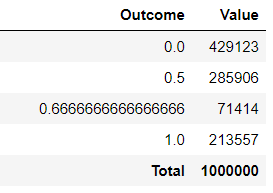
\includegraphics[width=0.91in,height=\textheight,keepaspectratio]{_graphics/mscoin-intro-table.png}

}

\subcaption{\label{fig-ms-coin-intro-plot-1}Table of observed values and
frequencies.}

\end{minipage}%
%
\begin{minipage}{0.50\linewidth}

\centering{

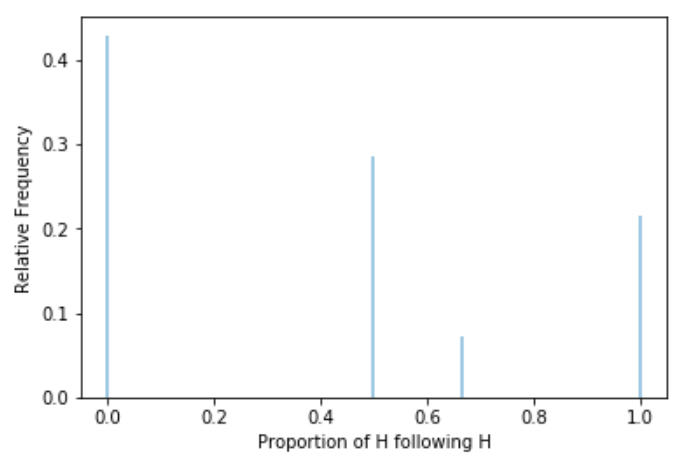
\includegraphics[width=2.28in,height=\textheight,keepaspectratio]{_graphics/mscoin-intro-plot.png}

}

\subcaption{\label{fig-ms-coin-intro-plot-2}Spike plot: heights of the
spikes represent the relative simulated relative frequencies of each
possible value of \emph{proportion of H followied by H} for a set of
four coin flips}

\end{minipage}%

\caption{\label{fig-ms-coin-intro-plot}Proportion of flips immediately
following H that result in H for 1,000,000 sets of 4 coin flips, each
set having at least one flip immediately following H. For example, the
\emph{proportion of H followed by H} is 0 in 429,123 of the sets.}

\end{figure}%

We asked the question: \emph{what would you expect} for the proportion
of the flips which immediately follow a H that result in H? That depends
on how we define what's ``expected''. If we are interested in the value
that is most likely to occur when we flip a coin four times, then the
answer is 0: we see that in the long run a little over 40\% of the sets
resulted in a proportion of 0, while only about 30\% of sets resulted in
a value of 1/2. We see that Figure~\ref{fig-ms-coin-intro-plot-2} is not
centered at 1/2; a higher percentage of repetitions resulted in a
proportion below 1/2 than above 1/2. We think that most people would
find this surprising.

Another way to interpret ``expected'' is as ``average''; in particular,
expected value can be interpreted as the long run average value. After
1,000,000 repetitions, each involving a set of four fair coin flips, we
have 1,000,000 simulated values of the proportion of H following H. We
could then average these values: add up all the values and divide by
1,000,000.

\[
{\scriptscriptstyle
\frac{0\times 429123 + (1/2)\times 285906 + (2/3) \times 71414 + 1 \times 213557}{1000000} = 0.404
}
\]

It turns out that the long run average value is 0.405, which is not 1/2.
Again, we think most people find this surprising.

A reminder: the term ``expected value'' is somewhat of a misnomer. We
are \emph{not} saying that if we flip a coin four times we would expect
the proportion of H following H for that set of flips to be 0.405. In
fact, in any single set of four fair coin flips the only possible values
for the proportion of H followed by H are 0, 1/2, 2/3, and 1. So in a
set of four coin flips it's not possible to see a proportion of 0.405.
Rather, 0.405 is the \emph{average value of the proportion of H followed
by H that we would expect to see in the long run over many sets of four
fair coin flips}.

The simulation provides evidence that, counter to our intuition, we
would expect the proportion of H followed by H to be \emph{less than
0.5}. So what is happening here? We will return to this example several
times to investigate these results more closely. We'll leave it as a
mystery for now, but observe that:

\begin{itemize}
\tightlist
\item
  The study of probability can involve some subtleties and our intuition
  isn't always right.
\item
  Simulation is an effective way of investigating probability problems,
  and can reveal interesting and surprising patterns.
\item
  There is a difference between (1) the probability that a flip
  following H lands on H and (2) the proportion of flips following H
  which result in H in a fixed sequence of fair coin flips\footnote{The
    probability that a flip following H lands on H is 0.5. This example
    shows that the proportion of flips following H which result in H in
    a fixed sequence of coin flips is a ``biased estimator'' of the
    probability that a flip following H lands on H.}.
\item
  In a fixed number of fair coin flips, the proportion of flips
  following H which result in H is ``expected'' to be less than the true
  probability of H, even though the trials are independent.
\end{itemize}

\subsection{Exercises}\label{exercises-7}

\begin{exercise}[]\protect\hypertarget{exr-literacy-birthday}{}\label{exr-literacy-birthday}

In a group of \(n\) people, what is the probability that at least two
people in the group people have the same birthday?

\begin{enumerate}
\def\labelenumi{\arabic{enumi}.}
\tightlist
\item
  Consider \(n=30\): what do you think the probability that at least two
  people in a group of 30 people share a birthday is: 0-20\%, 20-40\%,
  40-60\%, 60-80\%, 80-100\%?
\item
  How large do you think \(n\) needs to be in order for the probability
  that at least two people share a birthday to be larger than 0.5?
\item
  We'll save the answer to these questions for later, but they turn out
  to be unintuitive to many people, and simulation can shed some light.
  Explain how, in principle, you might perform a simulation using cards
  or slips of paper to estimate the probability that at least two people
  have the same birthday when \(n=30\). You can make some simplifying
  assumptions: Ignore multiple births and February 29 and assume that
  the other 365 days are all equally likely\footnote{Which isn't
    \href{https://visme.co/blog/most-common-birthday/}{quite}
    \href{http://thedailyviz.com/2016/09/17/how-common-is-your-birthday-dailyviz/}{true}.}.
\end{enumerate}

\end{exercise}

\section{Why study coins, dice, cards, and
spinners?}\label{sec-why-toys}

Many probability problems involve ``toy'' situations like flipping
coins, rolling dice, shuffling cards, or spinning spinners. These
situations might seem unexciting, or at least not very practically
meaningful. However, coins and spinners and the like provide familiar,
concrete situations which facilitate understanding of probability
concepts. Furthermore, simple situations often provide insight into real
and complex problems. The following is just one illustration.

Many basketball players and fans alike believe in the ``hot hand''
phenomenon: the idea that making several shots in a row increases a
player's chances of making the next shot. However, the consensus
conclusion of thirty years of studies on the hot hand, beginning with
the seminal study Gilovich, Vallone, and Tversky (1985), had been that
there is no statistical evidence that the hot hand in basketball is
real. As a result, many statisticians regularly caution against the
``hot hand fallacy'': the belief that the hot hand exists when, in
reality, the degree of streaky behavior typically observed in sequential
data is consistent with what would be expected simply by chance in
independent trials.

The idea behind studies like Gilovich, Vallone, and Tversky (1985) is
essentially the following. Consider a player who attempts 100 shots and
makes 50\%. If there is no hot hand, then we might expect the player to
make 50\% of shots both on attempts that follow hit streaks--- usually
considered three (or more) made attempts in a row---and on other
attempts. Therefore, a success rate of 50\% on both sets of attempts
provides no evidence of the hot hand.

However, recent research of Miller and Sanjurjo (2018a), Miller and
Sanjurjo (2018c), Miller and Sanjurjo (2018b) concludes that previous
studies on the hot hand in basketball, starting with Gilovich, Vallone,
and Tversky (1985), have been subject to a bias. After correcting for
the bias, the authors find evidence in favor of the hot hand effect in
basketball shooting, suggesting the hot hand fallacy is not a fallacy
after all. One interesting aspect of these studies is that Miller and
Sanjurjo's methods are simulation-based.

Miller and Sanjurjo (2018a) introduced the coin flipping problem in
Section Section~\ref{sec-sim}) to illustrate the idea behind their
research and the bias in previous studies. Consider again a player who
attempts 100 shots and makes 50\%. Even if there is no hot hand, Miller
and Sanjurjo show that we would actually expect the player to have a
shooting percentage of \emph{strictly less than} 50\% on the attempts
which followed streaks, and strictly greater than 50\% on the other
attempts. The reason is similar to what we observed in the the coin
flipping problem in Section~\ref{sec-sim}: in a fixed number of trials,
the proportion of H on trials following H is expected to be less than
the true probability of H, even though the trials are independent.
Therefore, for the example player a success rate of 50\% on both sets of
attempts actually provides directional evidence in favor of the hot
hand. Properly acccounting for this bias leads to substantially
different statistical analyses (i.e., p-values) and conclusions.

\subsection{Exercises}\label{exercises-8}

\begin{exercise}[]\protect\hypertarget{exr-literacy-why-spinners}{}\label{exr-literacy-why-spinners}

Find the value of some probability in a real world situation of interest
to you. Then describe how this situation could be modeled with coins,
dice, cards, or spinners. How would you use your ``toys'' to simulate
the situation and approximate the probability of interest?

\end{exercise}

\section{Chapter exercises}\label{chapter-exercises}

\begin{exercise}[]\protect\hypertarget{exr-TF1}{}\label{exr-TF1}

True or false.

\begin{enumerate}
\def\labelenumi{\arabic{enumi}.}
\tightlist
\item
  Probability can be used to assess the likelihood or plausibility of an
  event associated with a phenomenon that only happens once.
\item
  Probability can be used to assess the likelihood of an event
  associated with a phenomenon that happended in the past.
\item
  The subjective and long run relative frequency interpretations of
  probability can be used interchangeably.
\item
  Suppose the probability that a randomly selected CP student has an
  internship this summer is 0.2, and the probability that a randomly
  selected CP student is taking at least one course this summer is 0.4.
  True false: the probability that a randomly selected CP student either
  has an internship or is taking at least one class (or both) must be
  0.6.
\item
  Suppose the probability that a randomly selected CP student has an
  internship this summer is 0.2, and the probability that a randomly
  selected CP student is taking at least one course this summer is 0.4.
  True false: the probability that a randomly selected CP student both
  has an internship and is taking at least one class must be 0.08.
\end{enumerate}

\end{exercise}

\begin{exercise}[]\protect\hypertarget{exr-SA1}{}\label{exr-SA1}

Short answer.

\begin{enumerate}
\def\labelenumi{\arabic{enumi}.}
\tightlist
\item
  Your subjective probability that the price of regular unleaded
  gasoline at your favorite gas station in SLO stays above \$5 per
  gallon throughout the next month is 0.95. How many times more likely
  than not is it for the price to stay above \$5 per gallon through the
  next month?
\item
  It is 3 times more likely than not that the high temperature tomorrow
  will be greater than 80 degrees F. What is the probability that the
  high temperature tomorrow will be greater than 80 degrees F?
\item
  Laszlo, Nadja, and Nandor are having a tournament. Guillermo thinks
  that Nandor is 3.5 times more likely to win than Nadja, and Nadja is 2
  times more likely to win than Lazlso. Find Guillermo's probability
  that Nandor wins.
\end{enumerate}

\end{exercise}

\begin{exercise}[]\protect\hypertarget{exr-which1}{}\label{exr-which1}

In each of the following, which of a or b is strictly greater? Or are
they equal? Or is there not enough information to decide? Explain your
reasoning.

\begin{enumerate}
\def\labelenumi{\arabic{enumi}.}
\item
  Surfing Californians

  \begin{enumerate}
  \def\labelenumii{\alph{enumii}.}
  \tightlist
  \item
    The probability that a randomly selected Californian likes to surf
  \item
    The probability that a randomly selected American is a Californian
    who likes to surf
  \item
    a and b are necessarily equal
  \item
    There is not enough information provided to decide whether a or b is
    strictly greater
  \end{enumerate}
\item
  Cal Poly graduates

  \begin{enumerate}
  \def\labelenumii{\alph{enumii}.}
  \tightlist
  \item
    The probability that a randomly selected Cal Poly graduate is a
    California resident
  \item
    The probability that a randomly selected California resident is a
    Cal Poly graduate
  \item
    a and b are necessarily equal
  \item
    There is not enough information provided to decide whether a or b is
    strictly greater
  \end{enumerate}
\item
  Flips a coin which is known to be fair six times and record the
  results in sequence

  \begin{enumerate}
  \def\labelenumii{\alph{enumii}.}
  \tightlist
  \item
    The probability that the first \emph{five} flips are, in order,
    HHHHH
  \item
    The probability that the first \emph{six} flips are, in order,
    HTTHTH
  \item
    a and b are necessarily equal
  \item
    There is not enough information provided to decide whether a or b is
    strictly greater
  \end{enumerate}
\item
  I catch my child hiding in the bathroom washing chocolate off her
  face. I ask what her what she's doing, and she says she just had to go
  the bathroom.

  \begin{enumerate}
  \def\labelenumii{\alph{enumii}.}
  \tightlist
  \item
    The probability that my child just went to the bathroom.
  \item
    The probability that my child just went to the bathroom and has
    secretly been eating chocolate cake.
  \item
    a and b are necessarily equal
  \item
    There is not enough information provided to decide whether a or b is
    strictly greater
  \end{enumerate}
\item
  Among American workers, 40\% have a college degree and 10\% belong to
  a labor union.

  \begin{enumerate}
  \def\labelenumii{\alph{enumii}.}
  \tightlist
  \item
    4\%
  \item
    The percentage of American workers who have a college degree and
    belong to a labor union.
  \item
    a and b are necessarily equal
  \item
    There is not enough information provided to decide whether a or b is
    strictly greater
  \end{enumerate}
\end{enumerate}

\end{exercise}

\begin{exercise}[]\protect\hypertarget{exr-right-dominance}{}\label{exr-right-dominance}

Suppose

\begin{itemize}
\tightlist
\item
  85\% of people have a dominant right hand.
\item
  75\% of people with a dominant right hand have a dominant right eye.
\item
  55\% of people who do not have a dominant right hand have a dominant
  right eye.
\end{itemize}

\begin{enumerate}
\def\labelenumi{\arabic{enumi}.}
\tightlist
\item
  What percent of people with a dominant eye have a dominant right hand?
\item
  What percent of people with a dominant right eye do not have a
  dominant right hand?
\item
  What percent of people without a dominant right eye have a dominant
  right hand?
\item
  What percent of people with a dominant right hand have a dominant
  right eye?
\item
  What percent of people have a dominant right eye and a dominant right
  hand?
\end{enumerate}

\end{exercise}

\bookmarksetup{startatroot}

\chapter{The Language of Probability}\label{sec-language-probability}

A phenomenon is \emph{random} if there are multiple potential
possibilities, and there is \emph{uncertainty} about which possibility
is realized. This chapter introduces the fundamental terminology and
objects of random phenomena, including

\begin{itemize}
\tightlist
\item
  Possible \textbf{outcomes} (possibilities) of the random phenomenon
\item
  Related \textbf{events} that could occur
\item
  \textbf{Random variables} which measure numeric quantities based on
  outcomes
\item
  \textbf{Probability measures} which assign degrees of likelihood or
  plausibility to events in a logically coherent way and reflect
  assumptions about the random phenomenon
\item
  \textbf{Distributions} of random variables which describe their
  pattern of variability, and can be summarized by \emph{percentiles},
  \emph{expected values}, \emph{standard deviations} (and
  \emph{variances}), and \emph{correlations} (and \emph{covariances}).
\item
  \textbf{Conditioning}, which involves revising probabilities and
  distributions to reflect additional information
\end{itemize}

Probability models put all of the above together. A \textbf{probability
model}\index{probability model} of a random phenomenon consists of a
sample space of possible outcomes, associated events and random
variables, and a probability measure which specifies probabilities of
events and determines distributions of random variables according to the
assumptions of the model and available information.

Throughout this chapter we will illustrate ideas using the following
examples.

\textbf{Total or best?} Roll a \emph{four}-sided\footnote{Why
  four-sided? Simply to make the number of possibilities a little more
  manageable. Rolling a four-sided die twice yields 16 possible pairs,
  while rolling a six-sided die yields 36 possible pairs.} die twice and
consider the sum and the larger of the two rolls (or the common roll if
a die). Not very exciting? Maybe, but it is a familiar, simple, and
concrete example. Also, a ``toy'' example can provide insight into more
interesting problems, such as the following. In many sports, a
competitor's final ranking is based on the results of multiple attempts.
Competitors in Olympic bobsled, for example, make four separate timed
runs on the same course and their ranking is based on their \emph{total}
time. Competitors in Olympic shot put make six throws, but their ranking
is based on their \emph{best} throw. In sports with multiple attempts,
how do the rankings compare if they are based on the total (or average)
over all attempts (as in bobsled) or on the best attempt (as is shot
put)?

\textbf{Matching problem.} A group of people all put their names in a
hat for a Secret Santa gift exchange. The names are shuffled and
everyone draws a name from the hat. We might be interested in questions
like: What is the probability that someone selects their own name? How
many people are expected to draw their own name? How do the answers to
these questions depend on the name of people in the group? This a is
version of a well known probability problem called the ``matching
problem''. The general setup involves \(n\) distinct ``objects'' labeled
\(1, \ldots, n\) which are placed in \(n\) distinct ``boxes'' labeled
\(1, \ldots, n\), with exactly one object placed in each box; for how
many objects does the label on the object match the label on the box it
is placed in?

\textbf{Meeting problem.} Several people plan to meet for lunch, but
their arrival times are uncertain. We might be interested in whether
they arrive within 15 minutes of one another, who arrives first and at
what time, or how long the first person to arrive needs to wait for the
others.

\textbf{Collector problem.} Each box of a brand of cereal contains a
single prize from a collection. We might be interested in how many boxes
we need to buy to complete the collection, or how many boxes we need to
buy to complete five collections (say one collection for each of five
kids), or which prize we get in the most boxes.

\textbf{Arrivals over time.} Customers enter a deli and take a number to
mark their place in line. When the deli opens the counter starts 0; the
first customer to arrive takes number 1, the second 2, etc. We record
the counter over time, continuously, as it changes as customers arrive.
We might be interested in the number of customers that arrive in some
window of time, the time between customer arrivals, or the amount of
time it takes for some number of customers to arrive. (And this is just
the arrivals; we might also be interested in questions which involve the
departures, such as: how much time a customer spends in the deli or how
many customers are in the deli at a certain time.)

Full disclosure: many of the examples in this chapter involve rather dry
tasks like discussing mathematical notation or listing elements of sets.
Also, some of the things we do in these examples are rarely done in
practice. So why bother? Many common mistakes in solving probability
problems arise from misunderstanding these foundational objects. We hope
that concrete---though sometimes uninteresting---examples foster
understanding of fundamental concepts.

This chapter introduces what the fundamental objects of probability are,
but not yet how to solve probability problems. Don't worry; we'll solve
many interesting problems in the remaining chapters. Think of this
chapter as introducing the ``language'' or ``grammar'' of probability.
When first learning to write, we learn the basic elements of sentences:
subjects, predicates, clauses, modifiers, etc. Understanding these
fundamental building blocks is essential to learning how to write well,
even if we don't explicitly identify the subject, the verb, etc., in
every sentence we write. Likewise, understanding the language of
probability is crucial to learning how to solve probability problems,
even if the language is sometimes unspoken.

\section{Outcomes}\label{sec-language-outcomes}

Probability models can be applied to any situation in which there are
multiple potential outcomes and there is uncertainty about which outcome
is realized. Due to the wide variety of types of random phenomena, an
\textbf{outcome} can be virtually anything:

\begin{itemize}
\tightlist
\item
  the result of a coin flip
\item
  the results of a sequence of coin flips
\item
  a shuffle of a deck of cards
\item
  the weather conditions tomorrow in your city
\item
  the path of a particular Atlantic hurricane
\item
  the daily closing price of a certain stock over the next 30 days
\item
  a noisy electrical signal
\item
  the result of a diagnostic medical test
\item
  a sample of car insurance polices
\item
  the customers arriving at a store
\item
  the result of an election
\item
  the next World Series champion
\item
  a play in a basketball game
\end{itemize}

And on and on. In particular, an outcome does \emph{not} have to be a
number.

The first step in defining a probability model for a random phenomenon
is to identify the \emph{possible} outcomes.

\begin{definition}[]\protect\hypertarget{def-sample-space}{}\label{def-sample-space}

The \textbf{sample space}\index{sample space} is the collection of all
possible outcomes of a random phenomenon.

\end{definition}

Mathematically, the sample space is a \emph{set} containing all possible
outcomes, while any individual outcome is an \emph{element} in the
sample space. The sample space is typically denoted\footnote{There is no
  one set of universally agreed on notation, but \(\Omega\) is commonly
  used. It is also common practice to use uppercase and lowercase
  letters to denote different objects, like \(\Omega\) versus
  \(\omega\).} \(\Omega\), the uppercase Greek letter ``Omega''. An
outcome is typically denoted \(\omega\), the lowercase Greek letter
``omega''; \(\omega\) denotes a generic outcome much like the symbol
\(u\) in \(\sqrt{u}\) denotes a generic input to the square root
function. We write \(\omega \in \Omega\) (read \(\in\) as ``in'' or ``an
element of'') to represent that \(\omega\) is a possible outcome of
sample space \(\Omega\).

The simplest random phenomena have just two distinct outcomes, in which
case the sample space is just a set with two elements, e.g.,
\(\Omega=\{\text{no}, \text{yes}\}\),
\(\Omega=\{\text{off}, \text{on}\}\), \(\Omega=\{0, 1\}\),
\(\Omega=\{-1, 1\}\). For example, the sample space for a single coin
flip could be \(\Omega = \{H, T\}\). If the coin lands on heads, we
observe the outcome \(\omega = H\); if tails we observe \(\omega=T\).

In simple examples we can describe the sample space by listing all
possible outcomes. However, constructing a list of all possible outcomes
is rarely done in practice. We do so here only to provide some concrete
examples of sample spaces. While a random phenomenon always has a
corresponding sample space, in most situations the sample space of
outcomes is at best only vaguely specified and can not be feasibly
enumerated.

\begin{tcolorbox}[enhanced jigsaw, opacityback=0, left=2mm, colframe=quarto-callout-note-color-frame, toprule=.15mm, breakable, colback=white, leftrule=.75mm, arc=.35mm, rightrule=.15mm, bottomrule=.15mm]

\begin{example}[]\protect\hypertarget{exm-dice-outcome}{}\label{exm-dice-outcome}

Roll a four-sided die twice, and record the result of each roll in
sequence. For example, a 3 on the first roll and a 1 on the second is
not the same outcome as a 1 on the first roll and a 3 on the second.

\begin{enumerate}
\def\labelenumi{\arabic{enumi}.}
\item
  Identify the sample space.
\item
  We might be interested in the sum of the two rolls. Explain why it is
  still advantageous to define the sample space as in the previous part,
  rather than as just \(2, \ldots, 8\).
\end{enumerate}

\end{example}

\end{tcolorbox}

\begin{tcolorbox}[enhanced jigsaw, opacityback=0, rightrule=.15mm, coltitle=black, colframe=quarto-callout-tip-color-frame, toprule=.15mm, colbacktitle=quarto-callout-tip-color!10!white, opacitybacktitle=0.6, left=2mm, toptitle=1mm, breakable, title={Solution (click to expand)}, bottomtitle=1mm, colback=white, leftrule=.75mm, titlerule=0mm, arc=.35mm, bottomrule=.15mm]

\begin{refsolution}
\leavevmode

\begin{enumerate}
\def\labelenumi{\arabic{enumi}.}
\item
  We simply enumerate all the possible outcomes: first roll is a 1 and
  second roll is a 1, first roll is a 1 and second roll is a 2, etc. The
  sample space consists of 16 possible ordered pairs of rolls, which we
  can display in a list or table. See Table~\ref{tbl-dice-outcome}; any
  row is a possible outcome, and the table contains all possible
  outcomes.

  We can write the sample space as a set of ordered pairs,
  \begin{align*}
  \Omega & = \{(1, 1), (1, 2), (1, 3), (1, 4),\\
  & \qquad (2, 1), (2, 2), (2, 3), (2, 4),\\
  & \qquad (3, 1), (3, 2), (3, 3), (3, 4),\\
  & \qquad (4, 1), (4, 2), (4, 3), (4, 4)\}.
  \end{align*} Any element of this set is a possible outcome \(\omega\).
  For example, the outcome \(\omega = (4, 2)\) occurs when the first
  roll is a 4 and the second roll is a 2.
\item
  Yes, we might be interested in the sum of the two dice. But we might
  also be interested in other things, like the larger of the two rolls,
  or if at least one 3 was rolled, or the result of the first roll.
  Knowing just the sum of the rolls does not provide as much information
  about the outcome of the random phenomenon as the sequence of
  individual rolls does.
\end{enumerate}

\label{sol-dice-outcome}

\end{refsolution}

\end{tcolorbox}

\begin{table}

\caption{\label{tbl-dice-outcome}Table representing the sample space of
two rolls of a four-sided die. Each row represents an outcome.}

\centering{

\centering
\begin{tabular}[t]{r|r}
\hline
First roll & Second roll\\
\hline
1 & 1\\
\hline
1 & 2\\
\hline
1 & 3\\
\hline
1 & 4\\
\hline
2 & 1\\
\hline
2 & 2\\
\hline
2 & 3\\
\hline
2 & 4\\
\hline
3 & 1\\
\hline
3 & 2\\
\hline
3 & 3\\
\hline
3 & 4\\
\hline
4 & 1\\
\hline
4 & 2\\
\hline
4 & 3\\
\hline
4 & 4\\
\hline
\end{tabular}

}

\end{table}%

A random phenomenon is modeled by a \emph{single} sample space. In
Example~\ref{exm-dice-outcome} there was a single sample space whose
outcomes represented the result of the \emph{pair} of rolls; in
particular, there was not a separate sample space for each of the
individual rolls\footnote{We could have written the sample space as the
  Cartesian product \(\Omega = \{1, 2, 3, 4\} \times\{1, 2, 3, 4\}\),
  where the first \(\{1, 2, 3, 4\}\) set in the product represents the
  result of the first roll (and similarly for the second). But this
  Cartesian product still represents a single set of ordered pairs, and
  it is that single set which is the sample space corresponding to
  outcomes of the pair of rolls.}. Whenever possible, a sample space
outcome should be defined to provide the maximum amount of information
about the outcome of random phenomenon.

Here's another concrete example where we can list all the outcomes in
the sample space. However, keep in mind that enumerating the sample
space is rarely done in practice.

\begin{tcolorbox}[enhanced jigsaw, opacityback=0, left=2mm, colframe=quarto-callout-note-color-frame, toprule=.15mm, breakable, colback=white, leftrule=.75mm, arc=.35mm, rightrule=.15mm, bottomrule=.15mm]

\begin{example}[]\protect\hypertarget{exm-matching-outcome}{}\label{exm-matching-outcome}

Consider the matching problem with \(n=4\). Label the objects 1, 2, 3,
4, and the spots 1, 2, 3, 4, with spot 1 the correct spot for object 1,
etc. Identify an appropriate sample space.

\end{example}

\end{tcolorbox}

\begin{tcolorbox}[enhanced jigsaw, opacityback=0, rightrule=.15mm, coltitle=black, colframe=quarto-callout-tip-color-frame, toprule=.15mm, colbacktitle=quarto-callout-tip-color!10!white, opacitybacktitle=0.6, left=2mm, toptitle=1mm, breakable, title={Solution (click to expand)}, bottomtitle=1mm, colback=white, leftrule=.75mm, titlerule=0mm, arc=.35mm, bottomrule=.15mm]

\begin{refsolution}
We can consider each outcome to be a particular placement of objects in
the spots. For example, one outcome is when object 3 is placed in spot
1, object 2 in spot 2, object 1 in spot 3, and object 4 in spot 4;
another is when object 3 is placed in spot 1, object 2 in spot 2, object
4 in spot 3, and object 1 in spot 4. The sample space consists of all
the possible arrangments of the object labels into the 4 spots. There
are 24 outcomes; see Table~\ref{tbl-matching-outcome}). Recording
outcomes in this way provides more information than if we had chosen the
sample space to correspond to, for example, the number of objects that
were placed in the correct spot.

Using set notation the sample space is \begin{align*}
\Omega & = \{1234, 1243, 1324, 1342, 1423, 1432 \\
  & \qquad 2134, 2143, 2314, 2341, 2413, 2431 \\
  & \qquad 3124, 3142, 3214, 3241, 3412, 3421 \\
  & \qquad 4123, 4132, 4213, 4231, 4312, 4321\}
\end{align*} For example, the outcome 3214 (or \((3, 2, 1, 4)\))
represents that object 3 is placed in spot 1, object 2 in spot 2, object
1 in spot 3, and object 4 in spot 4.

\label{sol-matching-outcome}

\end{refsolution}

\end{tcolorbox}

\begin{longtable}[]{@{}rrrr@{}}

\caption{\label{tbl-matching-outcome}Table representing the sample space
in the matching problem with \(n=4\). Each row represents an outcome.}

\tabularnewline

\toprule\noalign{}
Spot 1 & Spot 2 & Spot 3 & Spot 4 \\
\midrule\noalign{}
\endhead
\bottomrule\noalign{}
\endlastfoot
1 & 2 & 3 & 4 \\
1 & 2 & 4 & 3 \\
1 & 3 & 2 & 4 \\
1 & 3 & 4 & 2 \\
1 & 4 & 2 & 3 \\
1 & 4 & 3 & 2 \\
2 & 1 & 3 & 4 \\
2 & 1 & 4 & 3 \\
2 & 3 & 1 & 4 \\
2 & 3 & 4 & 1 \\
2 & 4 & 1 & 3 \\
2 & 4 & 3 & 1 \\
3 & 1 & 2 & 4 \\
3 & 1 & 4 & 2 \\
3 & 2 & 1 & 4 \\
3 & 2 & 4 & 1 \\
3 & 4 & 1 & 2 \\
3 & 4 & 2 & 1 \\
4 & 1 & 2 & 3 \\
4 & 1 & 3 & 2 \\
4 & 2 & 1 & 3 \\
4 & 2 & 3 & 1 \\
4 & 3 & 1 & 2 \\
4 & 3 & 2 & 1 \\

\end{longtable}

In the two previous examples, the sample space was \textbf{discrete}, in
the sense that the outcomes could be enumerated in a list (though it
could be a very long list). But in many cases, it is not possible to
enumerate outcomes in a list, even in principle.

For example, consider the circular spinner (like from a kids game) in
Figure~\ref{fig-uniform-spinner}. Imagine a needle anchored at the
center of the circle which is spun and eventually lands pointing at a
number on the outside of the circle. The values in the picture are
rounded to two decimal places, but consider an idealized model where the
spinner is infinitely precise and the needle infinitely fine so that any
real number between 0 and 1 is a possible outcome. The sample space
corresponding to a single spin of this spinner is the
interval\footnote{Why have we started with {[}0, 1{]} and not some other
  continuous interval? Because probabilities take values in \([0, 1]\).
  We will see why this is useful in more detail later.} {[}0, 1{]}.
There are uncountably many numbers in {[}0, 1{]} so it would not be
possible to enumerate them in a list. The interval {[}0, 1{]} is an
example of a \textbf{continuous} sample space.

\begin{figure}

\centering{

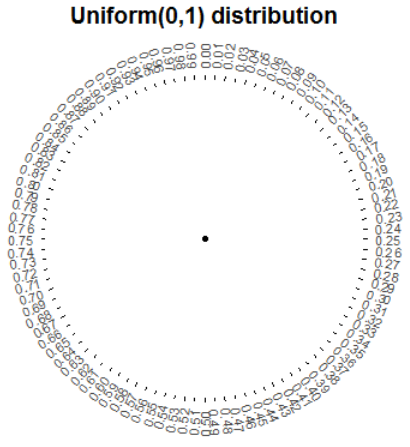
\includegraphics[width=1.37in,height=\textheight,keepaspectratio]{_graphics/uniform-spinner.png}

}

\caption{\label{fig-uniform-spinner}A continuous uniform spinner on
{[}0, 1{]}. The values in the picture are rounded to two decimal places,
but in the idealized model the spinner is infinitely precise so that any
real number between 0 and 1 is a possible outcome.}

\end{figure}%

\begin{tcolorbox}[enhanced jigsaw, opacityback=0, left=2mm, colframe=quarto-callout-note-color-frame, toprule=.15mm, breakable, colback=white, leftrule=.75mm, arc=.35mm, rightrule=.15mm, bottomrule=.15mm]

\begin{example}[]\protect\hypertarget{exm-meeting-outcome}{}\label{exm-meeting-outcome}

Consider a version of the meeting problem where two people. Regina and
Cady, will each definitely arrive between noon and 1, but their exact
arrival times are uncertain. Rather than dealing with clock time, it is
helpful to represent noon as time 0 and measure time as minutes after
noon, including fractions of a minute, so that arrival times take values
in the continuous interval {[}0, 60{]}.

Describe an appropriate sample space. Hint: it might be easiest to draw
a picture.

\end{example}

\end{tcolorbox}

\begin{tcolorbox}[enhanced jigsaw, opacityback=0, rightrule=.15mm, coltitle=black, colframe=quarto-callout-tip-color-frame, toprule=.15mm, colbacktitle=quarto-callout-tip-color!10!white, opacitybacktitle=0.6, left=2mm, toptitle=1mm, breakable, title={Solution (click to expand)}, bottomtitle=1mm, colback=white, leftrule=.75mm, titlerule=0mm, arc=.35mm, bottomrule=.15mm]

\begin{refsolution}
We can represent an outcome as a (Regina, Cady) pair of arrival times,
each in {[}0, 60{]}. For example, the outcome (30, 45.2) represents
Regina arriving at 12:30:00 and Cady at 12:45:12, while (45.2, 0)
represents Regina arriving at time (12:45:12) and Cady at noon. The
sample space is the set of all possible pairs.
Figure~\ref{fig-meeting-independent-uniform} displays the sample
space\footnotemark{} as the set of points within the colored square with
{[}0, 60{]} sides.

\label{sol-meeting-outcome}

\end{refsolution}

\end{tcolorbox}

\footnotetext{Mathematically we can write the sample space as
\([0,60]\times [0,60]=[0,60]^2\), the Cartesian product
\(\{(x, y): x \in [0, 60], y \in [0, 60]\}\), the set of ordered pairs
whose components take values in \([0, 60]\).}

\begin{figure}

\centering{

\pandocbounded{\includegraphics[keepaspectratio]{language-probability_files/figure-pdf/fig-meeting-independent-uniform-1.png}}

}

\caption{\label{fig-meeting-independent-uniform}The square represents
the sample space in Example~\ref{exm-meeting-outcome}). Each point
within the square is a (Regina, Cady) pair of arrival times in
\([0, 60]\).}

\end{figure}%

In the previous example, outcomes were measured on a continuous scale;
any real number between 0 and 60 was a possible arrival time. In
practice we might round the arrival time to the nearest minute or
second, but in principle and with infinite precision any real number in
the continuous interval \([0, 60]\) is possible.

Furthermore, even in situations where outcomes are inherently discrete,
it is often more convenient to model them as continuous. For example, if
an outcome represents the annual salary in dollars of a randomly
selected U.S. household, it would be more convenient to model the sample
space as the continuous interval\footnote{We could also try \([0, m]\)
  where \(m\) is some large dollar amount providing an upper bound on
  the maximum possible salary. But we would need to be sure that \(m\)
  is large enough so that all possible outcomes are in the sample space
  \([0, m]\). Without knowing this bound in advance, it is convenient to
  just choose the unbounded interval \([0, \infty)\). There is really no
  harm in making the sample space bigger than it needs to be, but you
  can run into problems if you make it too small.} \([0, \infty)\)
rather than discrete intervals like \(\{0, 1, 2, \ldots\}\) or
\(\{0, 0.01, 0.02, \ldots\}\). Continuous models are often more
tractable mathematically than discrete models.

\begin{tcolorbox}[enhanced jigsaw, opacityback=0, left=2mm, colframe=quarto-callout-note-color-frame, toprule=.15mm, breakable, colback=white, leftrule=.75mm, arc=.35mm, rightrule=.15mm, bottomrule=.15mm]

\begin{example}[]\protect\hypertarget{exm-collector-outcome}{}\label{exm-collector-outcome}

Consider the collector problem with 3 prizes in the collection, labeled
1, 2, and 3. We open boxes one at a time. Identify an appropriate sample
space. Is it possible to identify a sample space in which all outcomes
have the same ``length''?

\end{example}

\end{tcolorbox}

\begin{tcolorbox}[enhanced jigsaw, opacityback=0, rightrule=.15mm, coltitle=black, colframe=quarto-callout-tip-color-frame, toprule=.15mm, colbacktitle=quarto-callout-tip-color!10!white, opacitybacktitle=0.6, left=2mm, toptitle=1mm, breakable, title={Solution (click to expand)}, bottomtitle=1mm, colback=white, leftrule=.75mm, titlerule=0mm, arc=.35mm, bottomrule=.15mm]

\begin{refsolution}
An outcome could represent the sequence of prizes we obtain in order.
For example, (2, 3, 3, 2, 2, 2, 3, 1) represents prize 2 in the first
box, prize 3 in the second and third boxes, prize 2 in the fourth, and
so on, completing a collection with prize 1 in the eighth box. Outcomes
recorded in this way can have different lengths if we only record the
boxes we open until we complete a collection; for example (2, 3, 1)
versus (2, 3, 3, 1) versus (2, 3, 3, 2, 1). However, it is often
convenient for sample space outcomes to have the same length.

We can define outcomes with the same ``length'' if we assume the process
continues indefinitely, that is, if we continue to open boxes even after
we complete a set. Now an outcome is an \emph{infinite} sequence, with
each component of the sequence taking a value of 1, 2, or 3; for
example, (2, 3, 3, 2, 2, 2, 3, 1, 2, 1, 1, 3, \(\ldots\)). Thus the
sample space\footnotemark{} is the set of all infinite sequences whose
components take values in \(\{1, 2, 3\}\). Outcomes of this sample space
all have the same ``length''---infinite. Moreover, this sample space
allows for a broader range of questions to be investigated. For example,
we might be interested in the number of packages needed to obtain 5
complete collections (which might be relevant if you have 5 kids and
they all want their own collection).

\label{sol-collector-outcome}

\end{refsolution}

\end{tcolorbox}

\footnotetext{Mathematically this sample space can be written as
\(\Omega=\{1, 2, 3\}^\infty\).}

In the previous examples, the sample space could be defined rather
explicitly, either by direct enumeration or using set notation (like a
Cartesian product). However, explicitly defining a sample space in a
compact way is often not possible, as in the following example.

\begin{tcolorbox}[enhanced jigsaw, opacityback=0, left=2mm, colframe=quarto-callout-note-color-frame, toprule=.15mm, breakable, colback=white, leftrule=.75mm, arc=.35mm, rightrule=.15mm, bottomrule=.15mm]

\begin{example}[]\protect\hypertarget{exm-PP-outcome}{}\label{exm-PP-outcome}

Customers enter a deli and take a number to mark their place in line.
When the deli opens the counter starts 0; the first customer to arrive
takes number 1, the second 2, etc. We record the counter over time,
continuously, as it changes as customers arrive. Time is measured in
minutes after the deli opens (time 0). How might you define an
appropriate sample space?

\end{example}

\end{tcolorbox}

\begin{tcolorbox}[enhanced jigsaw, opacityback=0, rightrule=.15mm, coltitle=black, colframe=quarto-callout-tip-color-frame, toprule=.15mm, colbacktitle=quarto-callout-tip-color!10!white, opacitybacktitle=0.6, left=2mm, toptitle=1mm, breakable, title={Solution (click to expand)}, bottomtitle=1mm, colback=white, leftrule=.75mm, titlerule=0mm, arc=.35mm, bottomrule=.15mm]

\begin{refsolution}
A sample space outcome could be represented as a path of the value of
the counter over time; a few such paths are illustrated in
Figure~\ref{fig-PP-outcome}. The horizontal axis represents time and the
vertical axis represents the number of customers that have arrived.
Notice the stairstep feature: a customer arrives and takes a number then
the counter stays on that number for some time (the flat spots) until
another customer arrives and the counter increases by one (the jumps).
In other words, an outcome is a nondecreasing \emph{function} mapping
the time interval \([0, \infty)\) to nonnegative integers
\(\{0, 1, 2, \ldots\}\), that only jumps by one unit at a time. The
sample space consists of all possible \emph{functions} of this form.

\label{sol-PP-outcome}

\end{refsolution}

\end{tcolorbox}

\begin{figure}

\begin{minipage}{0.33\linewidth}

\centering{

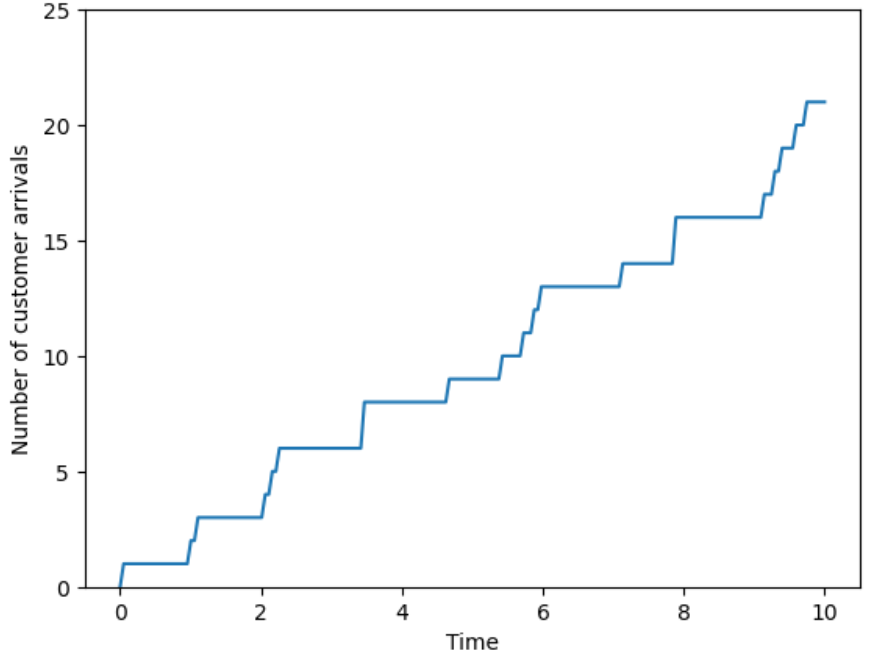
\includegraphics[width=2.91in,height=\textheight,keepaspectratio]{_graphics/PP-outcome-single.png}

}

\subcaption{\label{fig-PP-outcome-1}A single sample path of the number
of customer arrivals over time.}

\end{minipage}%
%
\begin{minipage}{0.33\linewidth}

\centering{

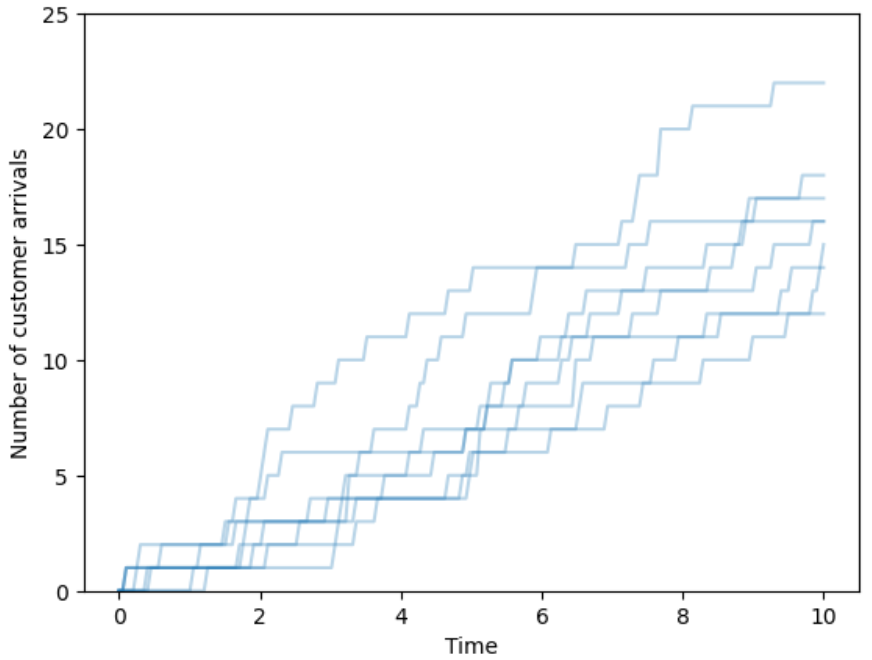
\includegraphics[width=2.91in,height=\textheight,keepaspectratio]{_graphics/PP-outcome-several.png}

}

\subcaption{\label{fig-PP-outcome-2}Several possible paths.}

\end{minipage}%
%
\begin{minipage}{0.33\linewidth}

\centering{

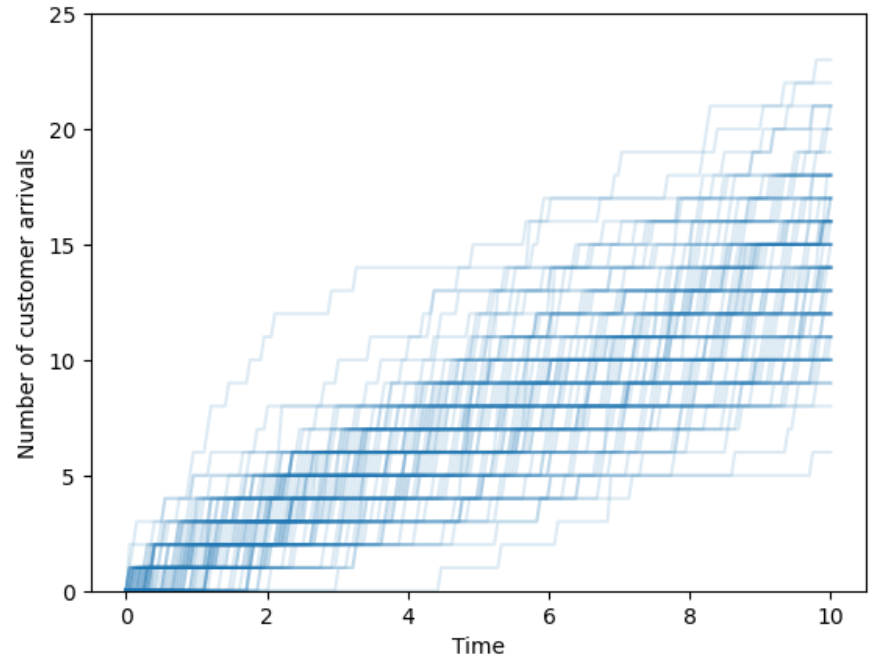
\includegraphics[width=2.92in,height=\textheight,keepaspectratio]{_graphics/PP-outcome-many.png}

}

\subcaption{\label{fig-PP-outcome-3}Many possible paths.}

\end{minipage}%

\caption{\label{fig-PP-outcome}Sample space outcomes for
Example~\ref{exm-PP-outcome}. Horizontal axes represent time and
vertical axes represent the number of customers that have arrived.}

\end{figure}%

Any random phenomenon has a corresponding sample space but in some
situations explicitly defining a outcome is not feasible. For example,
suppose the random phenomenon is tomorrow's weather. In order to
describe an outcome, we need to specify (among other things):
temperature, atmospheric pressure, wind, humidity, precipitation, and
cloudiness, and how it all evolves over over the course of tomorrow,
possibly in multiple locations. Representing all of this information in
a compact way to define even just one outcome is virtually impossible;
explicitly defining a sample space of all possible outcomes is hopeless.
Regardless, the sample space is still there in the background whether we
specify it or not.

Even though the sample space often is at best vaguely defined
(``tomorrow's weather'') and plays a background role, it is important to
first consider what is \emph{possible} before determining how
\emph{probable} events are. The sample space essentially defines the
denominator in probability calculations. In particular, considering the
sample space can help distinguish between ``the particular and the
general'' (as discussed in Section~\ref{sec-probofwhat}).

\subsection{Counting outcomes}\label{counting-outcomes}

When there are finitely many possibilities, we can ask: how many
possible outcomes are there? In Example~\ref{exm-dice-outcome} and
Example~\ref{exm-matching-outcome} we counted outcomes by enumerating
them in a list. Of course, listing all the outcomes is unfeasible unless
the sample space is very small. Now we'll see a simple principle that
can be applied to count outcomes.

\begin{tcolorbox}[enhanced jigsaw, opacityback=0, left=2mm, colframe=quarto-callout-note-color-frame, toprule=.15mm, breakable, colback=white, leftrule=.75mm, arc=.35mm, rightrule=.15mm, bottomrule=.15mm]

\begin{example}[]\protect\hypertarget{exm-counting-icecream}{}\label{exm-counting-icecream}

A soft serve ice cream shop has three flavors: vanilla, chocolate, or
swirl. Customers can choose to have a cone or a bowl.

\begin{enumerate}
\def\labelenumi{\arabic{enumi}.}
\tightlist
\item
  How can you determine the number of different ways the ice cream can
  be served? (Two possible ways are vanilla in a cone and chocolate in a
  bowl).
\item
  Customers can also add rainbow or chocolate sprinkles\footnotemark{}
  or not. Now how many different ways can the ice cream be served?
\item
  Customers who request bowls can choose to add whipped cream. Is the
  number of different ways the ice cream can be served equal to the
  answer to the previous part multiplied by two?
\end{enumerate}

\end{example}

\end{tcolorbox}

\footnotetext{a.k.a.,
\href{https://billypenn.com/2017/03/20/jimmies-vs-sprinkles-why-philly-fights-over-what-we-call-an-ice-cream-topping/}{jimmies}}

\begin{tcolorbox}[enhanced jigsaw, opacityback=0, rightrule=.15mm, coltitle=black, colframe=quarto-callout-tip-color-frame, toprule=.15mm, colbacktitle=quarto-callout-tip-color!10!white, opacitybacktitle=0.6, left=2mm, toptitle=1mm, breakable, title={Solution (click to expand)}, bottomtitle=1mm, colback=white, leftrule=.75mm, titlerule=0mm, arc=.35mm, bottomrule=.15mm]

\begin{refsolution}
\leavevmode

\begin{enumerate}
\def\labelenumi{\arabic{enumi}.}
\tightlist
\item
  Each flavor can be served in 2 ways, cone or bowl. Since there are 3
  flavors, the number of ways to serve is \(2+2+2 = 3\times2 = 6\).
\item
  Each of the 6 pairs from the previous part can be served in 3 ways,
  with rainbow sprinkles, with chocolate sprinkles, or without
  sprinkles. So the number of ways to serve is now
  \(3\times 2 \times 3 = 18\).
\item
  No.~Only the bowls can get whipped cream so we can't just multiply 18
  by 2. Of the 18 possibilities from the previous part, 9 are in bowls.
  So these 9 can be served with or without whipped cream, but the other
  9 in cones can only be served without whipped cream. The number of
  possibilities is now \(9\times 2 + 9 = 27\).
\end{enumerate}

\label{sol-counting-icecream}

\end{refsolution}

\end{tcolorbox}

All of the counting rules we will see are based on multiplying like in
Example~\ref{exm-counting-icecream}.

\begin{lemma}[Multiplication principle for
counting]\protect\hypertarget{lem-multiplication-principle}{}\label{lem-multiplication-principle}

Suppose that stage 1 of a process can be completed in any one of \(n_1\)
ways. Further, suppose that for each way of completing the stage 1,
stage 2 can be completed in any one of \(n_2\) ways. Then the two-stage
process can be completed in any one of \(n_1\times n_2\) ways. This rule
extends naturally to a \(\ell\)-stage process, which can then be
completed in any one of
\(n_1\times n_2\times n_3\times\cdots\times n_\ell\) ways.

\end{lemma}

In the multiplication principle it is not important whether there is a
``first'' or ``second'' stage. What is important is that there are
distinct stages, each with its own number of ``choices''. In
Example~\ref{exm-counting-icecream}, there was a bowl/cone stage, an ice
cream flavor stage, and a sprinkle stage; it didn't matter if the flavor
was chosen first or second or third.

We can use the multiplication principle to verify the total number of
possible outcomes for a few of our previous examples. In
Example~\ref{exm-dice-outcome} an outcome is a pair (first roll, second
roll). There are 4 possibilities for the first roll and 4 for the
second, so \(4\times4 = 16\) possible pairs. In
Example~\ref{exm-matching-outcome} an outcome is an arrangement of the 4
outcomes in the 4 spots. There are 4 possibilities for the object placed
in spot 1. After placing that object, there are 3 possibilities for spot
2, then 2 possibilities for spot 3, with one object left for spot 4. So
there are \(4\times3\times2\times1 = 24\) possible arrangements.

\begin{tcolorbox}[enhanced jigsaw, opacityback=0, left=2mm, colframe=quarto-callout-note-color-frame, toprule=.15mm, breakable, colback=white, leftrule=.75mm, arc=.35mm, rightrule=.15mm, bottomrule=.15mm]

\begin{example}[]\protect\hypertarget{exm-multiplication-rule-outcomes}{}\label{exm-multiplication-rule-outcomes}

Use the multiplication principle to count the total number of possible
outcomes in each of the following situations.

\begin{enumerate}
\def\labelenumi{\arabic{enumi}.}
\tightlist
\item
  Roll a six-sided die three times and record the result of each roll in
  sequence
\item
  Roll a four-sided die and a six-sided die and record the result of
  each roll.
\item
  Flip a coin four times and record the result of each flip in sequence
\item
  The number of arrangements of the objects in the matching problem with
  \(n=10\).
\item
  The number of possible draws in Example~\ref{exm-harry-second}.
\end{enumerate}

\end{example}

\end{tcolorbox}

\begin{tcolorbox}[enhanced jigsaw, opacityback=0, rightrule=.15mm, coltitle=black, colframe=quarto-callout-tip-color-frame, toprule=.15mm, colbacktitle=quarto-callout-tip-color!10!white, opacitybacktitle=0.6, left=2mm, toptitle=1mm, breakable, title={Solution (click to expand)}, bottomtitle=1mm, colback=white, leftrule=.75mm, titlerule=0mm, arc=.35mm, bottomrule=.15mm]

\begin{refsolution}
\leavevmode

\begin{enumerate}
\def\labelenumi{\arabic{enumi}.}
\tightlist
\item
  An outcome is a sequence of the results of each of the 3 flips. There
  are six possibilities for each roll, so \(6\times6\times6= 6^3=216\)
  possible outcomes.
\item
  There are 4 possibilities for one roll and 6 possibilities for the
  other, so there are \(4\times 6 = 24\) possible outcomes.
\item
  An outcome is a sequence of the H/T results of each of the 4 flips.
  There are two possibilities for each flip, so
  \(2\times2\times2\times2 = 2^4=16\) possible outcomes.
\item
  There are 10 objects that could potentially go in spot 1, then 9
  objects that could potentially go in spot 2, 8 to spot 3, and so on,
  with 1 left for spot 10. This results in
  \(10\times9\times8\times\cdots\times1=10! = 3,628,800\) possible
  outcomes. (That's over 3.6 million possibilities; we certainly
  wouldn't want to make a table!)
\item
  There are 5 possibilities for the first draw, then 4 possibilities for
  the second. If we record the outcome as the (first draw, second draw)
  result, there are \(5\times4 = 20\) possible outcomes.
\end{enumerate}

\label{sol-multiplcation-rule-outcomes}

\end{refsolution}

\end{tcolorbox}

The multiplication principle provides the foundation for some other
counting rules we will see later.

\subsection{Exercises}\label{exercises-9}

\begin{exercise}[]\protect\hypertarget{exr-coin4-outcome}{}\label{exr-coin4-outcome}

Consider the outcome of a sequence of 4 flips of a coin.

\begin{enumerate}
\def\labelenumi{\arabic{enumi}.}
\tightlist
\item
  Without enumerating the sample space, determine the number of
  outcomes.
\item
  Enumerate the sample space and confirm the number of outcomes.
\item
  We might be interested in the number of flips that land on heads.
  Explain why it is still advantageous to define the sample space as in
  the previous part, rather than as \(\Omega=\{0, 1, 2, 3, 4\}\).
\end{enumerate}

\end{exercise}

\begin{exercise}[]\protect\hypertarget{exr-collector4-outcome}{}\label{exr-collector4-outcome}

The latest series of collectible Lego Minifigures contains 3 different
Minifigure prizes (labeled 1, 2, 3). Each package contains a single
unknown prize. Suppose we only buy 3 packages and we consider as our
sample space outcome the results of just these 3 packages (prize in
package 1, prize in package 2, prize in package 3). For example, 323 (or
(3, 2, 3)) represents prize 3 in the first package, prize 2 in the
second package, prize 3 in the third package.

\begin{enumerate}
\def\labelenumi{\arabic{enumi}.}
\tightlist
\item
  Without enumerating the sample space, determine the number of
  outcomes.
\item
  Enumerate the sample space and confirm the number of outcomes.
\end{enumerate}

\end{exercise}

\section{Events}\label{sec-language-events}

An event is something that might happen or might be true. For example,
if we're interested in the weather conditions in our city tomorrow,
events include

\begin{itemize}
\tightlist
\item
  it rains
\item
  it does not rain
\item
  the high temperature is 75°F (rounded to the nearest °F)
\item
  the high temperature is above 75°F
\item
  it rains and the high temperature is above 75°F
\item
  it does not rain or the high temperature is not above 75°F
\end{itemize}

There are many possible outcomes for tomorrow's weather, but each of the
above will be true only for certain outcomes.

\begin{definition}[]\protect\hypertarget{def-event}{}\label{def-event}

An \textbf{event}\index{event} is a \emph{subset} of the sample space.
An event represents a collection of outcomes that some criteria.

\end{definition}

The sample space is the collection of all possible outcomes; an event
represents only those outcomes which satisfy some criteria. Events are
typically denoted with capital letters near the start of the alphabet,
with or without subscripts (e.g.~\(A\), \(B\), \(C\), \(A_1\), \(A_2\)).

Mathematically, events are sets, so events can be composed from others
using
\href{https://en.wikipedia.org/wiki/Set_(mathematics)\#Basic_operations}{basic
set operations} like unions (\(A\cup B\)), intersections (\(A \cap B\)),
and complements (\(A^c\)).

\begin{itemize}
\tightlist
\item
  \emph{Complements}. Read \(A^c\) as ``not \(A\)'', the outcomes that
  do not satisfy \(A\)
\item
  \emph{Intersections}. Read \(A\cap B\) as ``\(A\) and \(B\)'', the
  outcomes that satisfy both \(A\) and \(B\)
\item
  \emph{Unions}. Read \(A \cup B\) as ``\(A\) or \(B\)'', the outcomes
  that satisfy \(A\) or \(B\). Unions (\(\cup\), ``or'') are always
  inclusive: \(A\cup B\) occurs if \(A\) occurs but \(B\) does not,
  \(B\) occurs but \(A\) does not, or both \(A\) and \(B\) occur. Note
  that the complement of a union is the intersection of the complements,
  and vice versa: \((A \cup B)^c = A^c \cap B^c\) and
  \((A \cap B)^c = A^c \cup B^c\),
\end{itemize}

In the weather example above we can write

\begin{itemize}
\tightlist
\item
  \(A\): it rains
\item
  \(B=A^c\): it does not rain
\item
  \(C\): the high temperature is 75°F (rounded to the nearest °F)
\item
  \(D\): the high temperature is above 75°F
\item
  \(E = A \cap D\): it rains and the high temperature is above 75°F
\item
  \(F = A^c \cup D^c = (A\cap D)^c = B\cap D^c = E^c\): it does not rain
  or the high temperature is not above 75°F
\end{itemize}

\begin{tcolorbox}[enhanced jigsaw, opacityback=0, left=2mm, colframe=quarto-callout-note-color-frame, toprule=.15mm, breakable, colback=white, leftrule=.75mm, arc=.35mm, rightrule=.15mm, bottomrule=.15mm]

\begin{example}[]\protect\hypertarget{exm-simple-event}{}\label{exm-simple-event}

Every year the NBA Draft Lottery is conducted to determine which
non-playoff teams will receive the top draft picks.
Table~\ref{tbl-nba-draft} displays the teams that participated in the
2023 NBA Draft Lottery (held on May 16, 2023) along with some team
statistics from the
\href{https://www.basketball-reference.com/leagues/NBA_2023.html}{2022-2023
season} and the number of previous NBA championships won by the
franchise (as of 2023).

Imagine it's early May 2023 and the lottery hasn't happened yet. The
lottery determines---at random---the top three picks, but we'll just
consider the team who wins the first pick in the 2023 draft. The sample
space is the 14 teams in Table~\ref{tbl-nba-draft}. Identify each of the
following events relating to the team that wins the top pick.

\begin{enumerate}
\def\labelenumi{\arabic{enumi}.}
\tightlist
\item
  \(A\), the team is in the Western Conference.
\item
  \(B\), the team has never won a championship.
\item
  \(C\), the team won fewer than 25 games (Wins) in the 2022-2023 season
\item
  \(D\), the team scored over 115 points per game (PPG) in the 2022-2023
  season
\item
  Identify and interpret \(A\cap B\)
\item
  Identify and interpret \(A \cap B \cap D\)
\item
  Identify and interpret \(A \cup B\)
\item
  Identify and interpret \(B^c\)
\end{enumerate}

\end{example}

\end{tcolorbox}

\begin{table}

\caption{\label{tbl-nba-draft}Teams in the 2023 NBA Draft Lottery}

\centering{

\centering
\begin{tabular}[t]{l|l|r|r|r|r|r|r|r|r|r}
\hline
Team & Conference & Championships & Wins & PPG & FG3 & FG3A & FG2 & FG2A & FT & FTA\\
\hline
Detroit Pistons & Eastern & 3 & 17 & 110.3 & 11.4 & 32.4 & 28.2 & 54.6 & 19.8 & 25.7\\
\hline
Houston Rockets & Western & 2 & 22 & 110.7 & 10.4 & 31.9 & 30.2 & 56.9 & 19.1 & 25.3\\
\hline
San Antonio Spurs & Western & 5 & 22 & 113.0 & 11.1 & 32.2 & 32.0 & 60.4 & 15.8 & 21.2\\
\hline
Charlotte Hornets & Eastern & 0 & 27 & 111.0 & 10.7 & 32.5 & 30.5 & 57.9 & 17.6 & 23.6\\
\hline
Portland Trail Blazers & Western & 1 & 33 & 113.4 & 12.9 & 35.3 & 27.6 & 50.1 & 19.6 & 24.6\\
\hline
Orlando Magic & Eastern & 0 & 34 & 111.4 & 10.8 & 31.1 & 29.8 & 55.2 & 19.6 & 25.0\\
\hline
Indiana Pacers & Eastern & 0 & 35 & 116.3 & 13.6 & 37.0 & 28.4 & 52.6 & 18.7 & 23.7\\
\hline
Washington Wizards & Eastern & 1 & 35 & 113.2 & 11.3 & 31.7 & 30.9 & 55.2 & 17.6 & 22.4\\
\hline
Utah Jazz & Western & 0 & 37 & 117.1 & 13.3 & 37.8 & 29.2 & 52.0 & 18.7 & 23.8\\
\hline
Dallas Mavericks & Western & 1 & 38 & 114.2 & 15.2 & 41.0 & 24.8 & 43.3 & 19.0 & 25.1\\
\hline
Chicago Bulls & Eastern & 6 & 40 & 113.1 & 10.4 & 28.9 & 32.1 & 57.9 & 17.6 & 21.8\\
\hline
Oklahoma City Thunder & Western & 1 & 40 & 117.5 & 12.1 & 34.1 & 31.0 & 58.5 & 19.2 & 23.7\\
\hline
Toronto Raptors & Eastern & 1 & 41 & 112.9 & 10.7 & 32.0 & 31.1 & 59.3 & 18.4 & 23.4\\
\hline
New Orleans Pelicans & Western & 0 & 42 & 114.4 & 11.0 & 30.1 & 31.1 & 57.5 & 19.3 & 24.4\\
\hline
\end{tabular}

}

\end{table}%

\begin{tcolorbox}[enhanced jigsaw, opacityback=0, rightrule=.15mm, coltitle=black, colframe=quarto-callout-tip-color-frame, toprule=.15mm, colbacktitle=quarto-callout-tip-color!10!white, opacitybacktitle=0.6, left=2mm, toptitle=1mm, breakable, title={Solution (click to expand)}, bottomtitle=1mm, colback=white, leftrule=.75mm, titlerule=0mm, arc=.35mm, bottomrule=.15mm]

\begin{refsolution}
We'll write each of the events as a set of teams, but you can also think
of each event as a subset of the rows of Table~\ref{tbl-nba-draft}.

\begin{enumerate}
\def\labelenumi{\arabic{enumi}.}
\tightlist
\item
  \(A = \{\text{Houston, San Antonio, Portland, Utah, Dallas, Oklahoma City, New Orleans}\}\)
\item
  \(B = \{\text{Charlotte, Orlando, Indiana, Utah, New Orleans}\}\)
\item
  \(C=\{\text{Detroit, Houston, San Antonio}\}\)
\item
  \(D = \{\text{Indiana, Utah, Oklahoma City}\}\)
\item
  \(A\cap B = \{\text{Utah, New Orleans}\}\) is the event that the team
  is in the Western Conference and has won no previous championships.
\item
  \(A \cap B \cap D=\{\text{Utah}\}\) is the event that the team is in
  the Western Conference, has won no previous championships, and scored
  over 115 points per game in the 2022-2023 season.
\item
  \(A \cup B=\{\text{Charlottle, Houston, San Antonio, Portland, Orlando, Indians, Utah, Dallas, Oklahoma City, New Orleans}\}\)
  is the event that the team is in the Western Conference or has won no
  previous championships. Notice that teams that satisfy both \(A\) and
  \(B\), Utah and New Orleans, are included but only once.
\item
  \(B^c=\{\text{Detroit, Houston, San Antonio, Portland, Washington, Dallas, Chicago, Oklahoma City, Toronto}\}\)
  is the event that the team has won at least one previous championship.
\end{enumerate}

\label{sol-simple-event}

\end{refsolution}

\end{tcolorbox}

In Example~\ref{exm-simple-event} notice that we ony said the winner was
determined ``at random''; we didn't mention how. ``At random'' only
implies that the winning team will be selected in a manner that involves
uncertainly. ``At random'' does \emph{not} necessarily imply that the 14
teams are equally likely. In fact, the 2023 NBA Draft Lottery was
weighted to give teams with fewer wins the previous season a greater
probability of winning the top pick. We'll return to this idea later.
For now, we're just defining some events that are \emph{possible}; later
we will consider how \emph{probable} they are.

If the outcomes of a sample space are represented by rows in a table,
then events are subsets of rows which satisfy some criteria.

\begin{tcolorbox}[enhanced jigsaw, opacityback=0, left=2mm, colframe=quarto-callout-note-color-frame, toprule=.15mm, breakable, colback=white, leftrule=.75mm, arc=.35mm, rightrule=.15mm, bottomrule=.15mm]

\begin{example}[]\protect\hypertarget{exm-dice-event}{}\label{exm-dice-event}

Roll a four-sided die twice, and record the result of each roll in
sequence. Using the sample space from Example~\ref{exm-dice-outcome},
identify the following events.

\begin{enumerate}
\def\labelenumi{\arabic{enumi}.}
\tightlist
\item
  \(A\), the event that the sum of the two dice is 4.
\item
  \(B\), the event that the sum of the two dice is at most 3.
\item
  \(C\), the event that the larger of the two rolls (or the common roll
  if a tie) is 3.
\item
  \(A\cap C\) (identify and interpret).
\item
  \(D\), the event that the first roll is a 3.
\item
  \(E\), the event that the second roll is a 3.
\item
  \(D \cap E\) (identify and interpret).
\item
  \(D \cup E\) (identify and interpret).
\item
  If the outcome is \((1, 3)\), which of the events above occurred?
\end{enumerate}

\end{example}

\end{tcolorbox}

\begin{tcolorbox}[enhanced jigsaw, opacityback=0, rightrule=.15mm, coltitle=black, colframe=quarto-callout-tip-color-frame, toprule=.15mm, colbacktitle=quarto-callout-tip-color!10!white, opacitybacktitle=0.6, left=2mm, toptitle=1mm, breakable, title={Solution (click to expand)}, bottomtitle=1mm, colback=white, leftrule=.75mm, titlerule=0mm, arc=.35mm, bottomrule=.15mm]

\begin{refsolution}
Remember that the sample space consists of 16 possible ordered pairs of
rolls, (first roll, second roll); see Table~\ref{tbl-dice-outcome}. All
events must be defined as subsets of this sample space.

\begin{enumerate}
\def\labelenumi{\arabic{enumi}.}
\tightlist
\item
  \(A\) consists of the outcomes (1, 3), (2, 2), and (3, 1). In set
  notation, event \(A\) is the set \(\{(1, 3), (2, 2), (3, 1)\}\). This
  event is highlighted in Table~\ref{tbl-dice-event}.
\item
  \(B\) consists of the outcomes (1, 1), (1, 2), and (2, 1). In set
  notation, \(B = \{(1, 1), (1, 2), (2, 1)\}\).
\item
  \(C\) consists of the outcomes (1, 3), (2, 3), (3, 1), (3, 2), and (3,
  3). In set notation,
  \(B = \{(1, 3), (2, 3), (3, 1), (3, 2), (3, 3)\}\).
\item
  \(A\cap C\), which consists of the outcomes (1, 3) and (3, 1), is the
  event that both the sum of the two dice is 4 and the larger of the two
  rolls is 3. In set notation, \(A \cap C = \{(1, 3), (3, 1)\}\).
\item
  Each outcome in the sample space consists of a pair of rolls, so we
  must account for both rolls in defining events, even if the event of
  interest involves just the first roll. (Remember, there is always a
  single sample space upon which all events are defined.) So \(D\)
  consists of the outcomes (3, 1), (3, 2), (3, 3), and (3, 4). In set
  notation, \(D = \{(3, 1), (3, 2), (3, 3), (3, 4)\}\).
\item
  \(E\) consists of the outcomes (1, 3), (2, 3), (3, 3), and (4, 3). In
  set notation, \(E = \{(1, 3), (2, 3), (3, 3), (4, 3)\}\). Note that
  this is not the same event as \(D\).
\item
  \(D \cap E\), which consists only of the outcome (3, 3), is the event
  that both rolls result in a 3. While an event is always a set, it can
  be a set consisting of a single outcome (or the empty set). In set
  notation, \(D\cap E = \{(3, 3)\}\).
\item
  \(D \cup E\), which consists of the outcomes (3, 1), (3, 2), (3, 3),
  (3, 4), (1, 3), (2, 3), and (4, 3) is the event that at least one of
  the two rolls results in a 3. In set notation,
  \(D \cup E = \{(3, 1), (3, 2), (3, 3), (3, 4), (1, 3), (2, 3), (4, 3)\}\).
  Notice that the union is inclusive: \((3, 3)\), the outcome that
  satisfies both \(D\) and \(E\), is an element of \(D\cup E\). But also
  notice that the outcome \((3, 3)\) only appears \emph{once} in
  \(D\cup E\).
\item
  If the outcome is \((1, 3)\) then events \(A\), \(C\), \(A\cap C\),
  \(E\), \(D\cup E\) all occur. Events \(B,\) \(D\) and \(D\cap E\) do
  not occur. The outcome \((1, 3)\) is an element of each of the sets
  \(A\), \(C\), \(A\cap C\), \(E\), \(D\cup E\), but not of \(B,\) \(D\)
  and \(D\cap E\).
\end{enumerate}

\label{sol-dice-event}

\end{refsolution}

\end{tcolorbox}

\begin{table}

\caption{\label{tbl-dice-event}Table representing the sample space of
two rolls of a four-sided die. The outcomes in orange comprise the event
\(A\), the sum is equal to 4.}

\centering{

\centering
\begin{tabular}[t]{r|r|r}
\hline
First roll & Second roll & Sum is 4?\\
\hline
1 & 1 & no\\
\hline
1 & 2 & no\\
\hline
\cellcolor[HTML]{FFA500}{\textcolor{white}{\textbf{1}}} & \cellcolor[HTML]{FFA500}{\textcolor{white}{\textbf{3}}} & \cellcolor[HTML]{FFA500}{\textcolor{white}{\textbf{yes}}}\\
\hline
1 & 4 & no\\
\hline
2 & 1 & no\\
\hline
\cellcolor[HTML]{FFA500}{\textcolor{white}{\textbf{2}}} & \cellcolor[HTML]{FFA500}{\textcolor{white}{\textbf{2}}} & \cellcolor[HTML]{FFA500}{\textcolor{white}{\textbf{yes}}}\\
\hline
2 & 3 & no\\
\hline
2 & 4 & no\\
\hline
\cellcolor[HTML]{FFA500}{\textcolor{white}{\textbf{3}}} & \cellcolor[HTML]{FFA500}{\textcolor{white}{\textbf{1}}} & \cellcolor[HTML]{FFA500}{\textcolor{white}{\textbf{yes}}}\\
\hline
3 & 2 & no\\
\hline
3 & 3 & no\\
\hline
3 & 4 & no\\
\hline
4 & 1 & no\\
\hline
4 & 2 & no\\
\hline
4 & 3 & no\\
\hline
4 & 4 & no\\
\hline
\end{tabular}

}

\end{table}%

We reiterate (again!) that there is a single sample space, upon which
all events are defined. In the above example, events that involved only
the first or second roll such as \(D\) and \(E\) were still defined in
terms of pairs of rolls. An outcome in a sample space should be defined
to record as much information as possible so that the occurrence or
non-occurrence of all events of interest can be determined.

Some events consist of a single outcome, or no outcomes at all (the
``empty set'' denoted \(\{\}\) or \(\emptyset\)).

\begin{definition}[]\protect\hypertarget{def-disjoint-events}{}\label{def-disjoint-events}

Events \(A_1, A_2. A_3, \ldots\) are \textbf{disjoint}\index{disjoint}
(a.k.a. mutually exclusive) if none of the events have any outcomes in
common; that is, if \(A_i \cap A_j = \emptyset\) for all \(i\neq j\).

\end{definition}

Roughly, disjoint events do not ``overlap''. In
Example~\ref{exm-dice-event}, events \(B\) and \(C\) are disjoint since
\(B \cap C = \emptyset\); there are no outcomes for which both the sum
of the dice is at most 3 and the larger roll is a 3.

\begin{tcolorbox}[enhanced jigsaw, opacityback=0, left=2mm, colframe=quarto-callout-note-color-frame, toprule=.15mm, breakable, colback=white, leftrule=.75mm, arc=.35mm, rightrule=.15mm, bottomrule=.15mm]

\begin{example}[]\protect\hypertarget{exm-matching-event}{}\label{exm-matching-event}

In the matching problem with \(n=4\) objects labeled 1, 2, 3, 4, are
placed in spots labeled 1, 2, 3, 4, with spot 1 the correct spot for
object 1, etc. Using the sample space from
Example~\ref{exm-matching-outcome}, identify the following events.

\begin{enumerate}
\def\labelenumi{\arabic{enumi}.}
\tightlist
\item
  \(A\), the event that all objects are put in the correct spot.
\item
  \(F\), the event that no objects are put in the correct spot.
\item
  \(D\), the event that exactly 3 objects are put in the correct spot.
\item
  \(A_3\), the event that object 3 is put (correctly) in spot 3.
\end{enumerate}

\end{example}

\end{tcolorbox}

\begin{tcolorbox}[enhanced jigsaw, opacityback=0, rightrule=.15mm, coltitle=black, colframe=quarto-callout-tip-color-frame, toprule=.15mm, colbacktitle=quarto-callout-tip-color!10!white, opacitybacktitle=0.6, left=2mm, toptitle=1mm, breakable, title={Solution (click to expand)}, bottomtitle=1mm, colback=white, leftrule=.75mm, titlerule=0mm, arc=.35mm, bottomrule=.15mm]

\begin{refsolution}
Recall that each outcome is a particular placement of objects in the
spots. For example, the outcome (3, 2, 1, 4)---which we'll shorten to
3214---signifies that object 3 is put in spot 1, object 2 in spot 2,
object 1 in spot 3, and object 4 in spot 4.

\begin{enumerate}
\def\labelenumi{\arabic{enumi}.}
\tightlist
\item
  There is only one outcome, 1234, for which all objects are put in the
  correct spot, so \(A=\{1234\}\). Remember that an event is always a
  set, but it can be a set consisting of a single outcome.
\item
  For each outcome in the sample space check to see if the criteria
  holds to identify
  \(F=\{2143, 2341, 2413, 3142, 3412, 3421, 4123, 4312, 4321\}\) as the
  event that no objects are put in the correct spot.
\item
  There are no outcomes in which exactly 3 objects are put in the
  correct spot so \(D=\emptyset\). (For \(n=4\), if three objects are in
  their correct spots, then the remaining object must be in its correct
  spot too.)
\item
  \(A_3=\{1234, 1432, 2134, 2431, 4132, 4231\}\) is the event that
  object 3 is put (correctly) in spot 3. This event is highlighted in
  Table~\ref{tbl-matching-event}. Even though event \(A_3\) only
  concerns object 3, since the sample space consists of the placements
  of each of the objects then all events must be expressed in terms of
  these outcomes.
\end{enumerate}

\label{sol-matching-event}

\end{refsolution}

\end{tcolorbox}

\begin{table}

\caption{\label{tbl-matching-event}Table representing the sample space
in the matching problem with \(n=4\). The outcomes in orange comprise
the event \(A_3\), object 3 in spot 3.}

\centering{

\centering
\begin{tabular}[t]{r|r|r|r|r}
\hline
Spot  1 & Spot  2 & Spot  3 & Spot  4 & Object 3 in spot 3?\\
\hline
\cellcolor[HTML]{FFA500}{\textcolor{white}{\textbf{1}}} & \cellcolor[HTML]{FFA500}{\textcolor{white}{\textbf{2}}} & \cellcolor[HTML]{FFA500}{\textcolor{white}{\textbf{3}}} & \cellcolor[HTML]{FFA500}{\textcolor{white}{\textbf{4}}} & \cellcolor[HTML]{FFA500}{\textcolor{white}{\textbf{yes}}}\\
\hline
1 & 2 & 4 & 3 & no\\
\hline
1 & 3 & 2 & 4 & no\\
\hline
1 & 3 & 4 & 2 & no\\
\hline
1 & 4 & 2 & 3 & no\\
\hline
\cellcolor[HTML]{FFA500}{\textcolor{white}{\textbf{1}}} & \cellcolor[HTML]{FFA500}{\textcolor{white}{\textbf{4}}} & \cellcolor[HTML]{FFA500}{\textcolor{white}{\textbf{3}}} & \cellcolor[HTML]{FFA500}{\textcolor{white}{\textbf{2}}} & \cellcolor[HTML]{FFA500}{\textcolor{white}{\textbf{yes}}}\\
\hline
\cellcolor[HTML]{FFA500}{\textcolor{white}{\textbf{2}}} & \cellcolor[HTML]{FFA500}{\textcolor{white}{\textbf{1}}} & \cellcolor[HTML]{FFA500}{\textcolor{white}{\textbf{3}}} & \cellcolor[HTML]{FFA500}{\textcolor{white}{\textbf{4}}} & \cellcolor[HTML]{FFA500}{\textcolor{white}{\textbf{yes}}}\\
\hline
2 & 1 & 4 & 3 & no\\
\hline
2 & 3 & 1 & 4 & no\\
\hline
2 & 3 & 4 & 1 & no\\
\hline
2 & 4 & 1 & 3 & no\\
\hline
\cellcolor[HTML]{FFA500}{\textcolor{white}{\textbf{2}}} & \cellcolor[HTML]{FFA500}{\textcolor{white}{\textbf{4}}} & \cellcolor[HTML]{FFA500}{\textcolor{white}{\textbf{3}}} & \cellcolor[HTML]{FFA500}{\textcolor{white}{\textbf{1}}} & \cellcolor[HTML]{FFA500}{\textcolor{white}{\textbf{yes}}}\\
\hline
3 & 1 & 2 & 4 & no\\
\hline
3 & 1 & 4 & 2 & no\\
\hline
3 & 2 & 1 & 4 & no\\
\hline
3 & 2 & 4 & 1 & no\\
\hline
3 & 4 & 1 & 2 & no\\
\hline
3 & 4 & 2 & 1 & no\\
\hline
4 & 1 & 2 & 3 & no\\
\hline
\cellcolor[HTML]{FFA500}{\textcolor{white}{\textbf{4}}} & \cellcolor[HTML]{FFA500}{\textcolor{white}{\textbf{1}}} & \cellcolor[HTML]{FFA500}{\textcolor{white}{\textbf{3}}} & \cellcolor[HTML]{FFA500}{\textcolor{white}{\textbf{2}}} & \cellcolor[HTML]{FFA500}{\textcolor{white}{\textbf{yes}}}\\
\hline
4 & 2 & 1 & 3 & no\\
\hline
\cellcolor[HTML]{FFA500}{\textcolor{white}{\textbf{4}}} & \cellcolor[HTML]{FFA500}{\textcolor{white}{\textbf{2}}} & \cellcolor[HTML]{FFA500}{\textcolor{white}{\textbf{3}}} & \cellcolor[HTML]{FFA500}{\textcolor{white}{\textbf{1}}} & \cellcolor[HTML]{FFA500}{\textcolor{white}{\textbf{yes}}}\\
\hline
4 & 3 & 1 & 2 & no\\
\hline
4 & 3 & 2 & 1 & no\\
\hline
\end{tabular}

}

\end{table}%

We can use the multiplication principle to count the number of outcomes
that satisfy event \(A_3\) in Table~\ref{tbl-matching-event}. If object
3 is in spot 3, there are 3 objects that can go in spot 1, then 2 that
can go in spot 2, leaving 1 for spot 4; for a total of
\(3\times2\times1\times1=6\) of the 24 outcomes which satisfy event
\(A_3\).

When more than just a few events are of interest, subscripts are
commonly used to identify different events. In the previous example, we
might also be interested in \(A_1\), the event that object 1 is placed
in spot 1; \(A_2\), the event that object 2 is placed in spot 2; and so
on.

Remember that intervals of real numbers such as \((a,b), [a,b], (a,b]\)
are also sets, and so can also be events. For example, if an outcome is
the result of a single spin of the spinner in
Figure~\ref{fig-uniform-spinner}, events include

\begin{itemize}
\tightlist
\item
  \([0, 0.5]\), the result is between 0 and 0.5 (the needle lands in the
  right half of the spinner)
\item
  \([0.75, 1]\), the result is between 0.75 and 1 (the needle lands in
  the northwest quarter of the spinner)
\item
  \([0.595, 0.605)\), the result rounded to two decimal places is 0.60
\item
  \(\{0.6\}\), the result is 0.6 exactly (the needle points exactly at
  0.60000000\(\ldots\))
\end{itemize}

It is often helpful to conceptualize and visualize events (sets) with
pictures, especially when dealing with continuous sample spaces.

\begin{tcolorbox}[enhanced jigsaw, opacityback=0, left=2mm, colframe=quarto-callout-note-color-frame, toprule=.15mm, breakable, colback=white, leftrule=.75mm, arc=.35mm, rightrule=.15mm, bottomrule=.15mm]

\begin{example}[]\protect\hypertarget{exm-meeting-event}{}\label{exm-meeting-event}

Using the sample space from Example~\ref{exm-meeting-outcome}, identify
the following events using pictures.

\begin{enumerate}
\def\labelenumi{\arabic{enumi}.}
\tightlist
\item
  \(A\), the event that Regina arrives after Cady.
\item
  \(B\), the event that either Regina or Cady arrives before 12:30.
\item
  \(C\), the event that Cady arrives first and Regina arrives at most 15
  minutes after Cady.
\item
  \(D\), the event that Regina arrives before 12:24.
\end{enumerate}

\end{example}

\end{tcolorbox}

\begin{tcolorbox}[enhanced jigsaw, opacityback=0, rightrule=.15mm, coltitle=black, colframe=quarto-callout-tip-color-frame, toprule=.15mm, colbacktitle=quarto-callout-tip-color!10!white, opacitybacktitle=0.6, left=2mm, toptitle=1mm, breakable, title={Solution (click to expand)}, bottomtitle=1mm, colback=white, leftrule=.75mm, titlerule=0mm, arc=.35mm, bottomrule=.15mm]

\begin{refsolution}
Figure~\ref{fig-meeting-independent-uniform} represents the sample
space, a square with \([0, 60]\) sides. Each point within the square is
a (Regina, Cady) pair of arrival times. We can shade the regions of the
sample space corresponding to pairs of points that satisfy these events.
See Figure~\ref{fig-meeting-event}.

\label{sol-meeting-event}

\end{refsolution}

\end{tcolorbox}

\begin{figure}

\centering{

\pandocbounded{\includegraphics[keepaspectratio]{language-probability_files/figure-pdf/fig-meeting-event-1.png}}

}

\caption{\label{fig-meeting-event}Depiction of the events in
Example~\ref{exm-meeting-event}.}

\end{figure}%

In Example~\ref{exm-meeting-event} the sample space consists of (Regina,
Cady) pairs of arrival times so any event must be expressed as a
collection of pairs. Even though the criteria for event \(D\) involves
only Regina's arrival time, the event is not simply {[}0, 24{]}; we need
to consider all (Regina, Cady) pairs for which the Regina component is
in the interval {[}0, 24{]}.

\begin{tcolorbox}[enhanced jigsaw, opacityback=0, left=2mm, colframe=quarto-callout-note-color-frame, toprule=.15mm, breakable, colback=white, leftrule=.75mm, arc=.35mm, rightrule=.15mm, bottomrule=.15mm]

\begin{example}[]\protect\hypertarget{exm-PP-event}{}\label{exm-PP-event}

Consider the sample space in Example~\ref{exm-PP-outcome}. Sketch a
picture representing \(A\), the event that no arrivals occur in the
first 5 minutes.

\end{example}

\end{tcolorbox}

\begin{tcolorbox}[enhanced jigsaw, opacityback=0, rightrule=.15mm, coltitle=black, colframe=quarto-callout-tip-color-frame, toprule=.15mm, colbacktitle=quarto-callout-tip-color!10!white, opacitybacktitle=0.6, left=2mm, toptitle=1mm, breakable, title={Solution (click to expand)}, bottomtitle=1mm, colback=white, leftrule=.75mm, titlerule=0mm, arc=.35mm, bottomrule=.15mm]

\begin{refsolution}
The sample space consists of all possible non-decreasing integer-valued
paths that start at 0 at time 0; a few outcomes are depicted in
Figure~\ref{fig-PP-event}. Only paths that result in 0 arrivals at time
5 satisfy event \(A\). Figure~\ref{fig-PP-event} highlights in orange a
few possible outcomes that satisfy event \(A\). Event \(A\) consists of
all paths that stay constant at 0 from time 0 until at least time 5.

\label{sol-PP-event}

\end{refsolution}

\end{tcolorbox}

\begin{figure}

\centering{

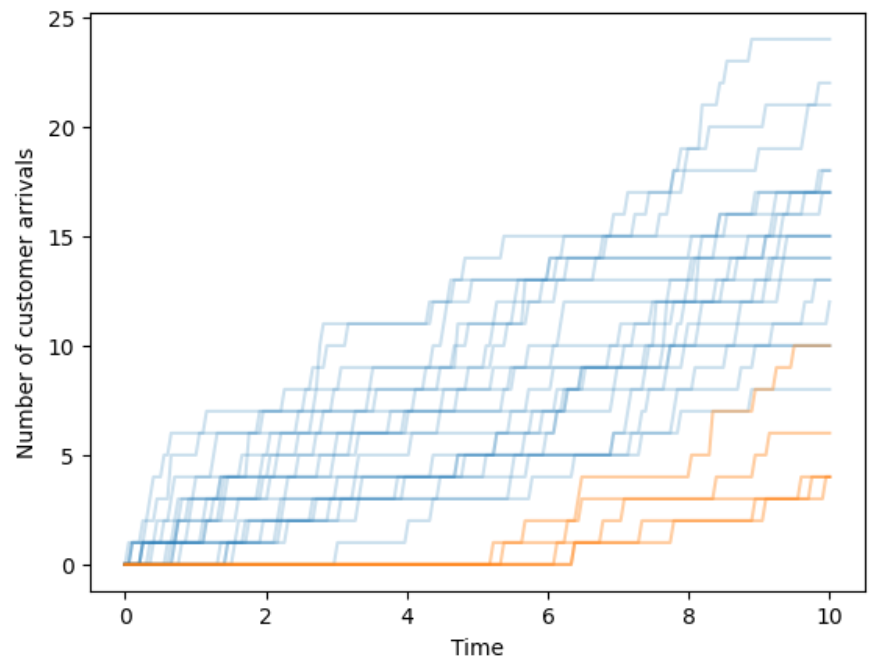
\includegraphics[width=2.92in,height=\textheight,keepaspectratio]{_graphics/PP-path-event.png}

}

\caption{\label{fig-PP-event}Sample space outcomes for
Example~\ref{exm-PP-event}. Paths in orange satisfy \(A\), the event
that no arrivals occur in the first 5 minutes; paths in blue do not
satisfy event \(A\).}

\end{figure}%

In many situations it is not possible to explicitly define a sample
space in a compact way, and so outcomes and events are often only
vaguely defined. Nevertheless, there is always a sample space in the
background representing possible outcomes, and collections of these
outcomes represent events of interest.

\begin{tcolorbox}[enhanced jigsaw, opacityback=0, left=2mm, colframe=quarto-callout-note-color-frame, toprule=.15mm, breakable, colback=white, leftrule=.75mm, arc=.35mm, rightrule=.15mm, bottomrule=.15mm]

\begin{example}[]\protect\hypertarget{exm-dd-event}{}\label{exm-dd-event}

Donny Don't is asked a series of questions involving a pair of rolls of
six-sided dice, such as ``identify the event that the sum of the dice is
at least 10''. Donny's responses are below; explain to him what is wrong
with his responses and help him understand the correct answers.

\begin{enumerate}
\def\labelenumi{\arabic{enumi}.}
\tightlist
\item
  The possible rolls are 1 through 6, so the sample space is
  \(\{1, 2, 3, 4, 5, 6\}\).
\item
  The sum of the two dice can be 2 through 12, so the event that the sum
  of the two dice is at least 10 is \(\{10, 11, 12\}\).
\item
  The event that the first roll is a 3 is \(\{3\}\).
\item
  The event that the first roll is a 3 and the second roll is a 1 is
  \(\{3, 1\}\)
\item
  Donny's sample space from the first question might correspond to what
  dice rolling scenario?
\item
  Donny says ``OK, I get that \(\{1, 2, 3, 4, 5, 6\}\) is the sample
  space for a \emph{single} roll of a six-sided die. But \(\{3, 1\}\)
  doesn't make any as an event because the die can't land on both 1 and
  3.'' Explain to Donny what the event \(\{3, 1\}\) represents in this
  scenario.
\end{enumerate}

\end{example}

\end{tcolorbox}

\begin{tcolorbox}[enhanced jigsaw, opacityback=0, rightrule=.15mm, coltitle=black, colframe=quarto-callout-tip-color-frame, toprule=.15mm, colbacktitle=quarto-callout-tip-color!10!white, opacitybacktitle=0.6, left=2mm, toptitle=1mm, breakable, title={Solution (click to expand)}, bottomtitle=1mm, colback=white, leftrule=.75mm, titlerule=0mm, arc=.35mm, bottomrule=.15mm]

\begin{refsolution}
\leavevmode

\begin{enumerate}
\def\labelenumi{\arabic{enumi}.}
\tightlist
\item
  The questions involve a pair of rolls, so best to record an outcome as
  an ordered pair, e.g., (5, 2) for 5 on the first roll and 2 on the
  second. Therefore, the sample space would be the following set of 36
  possible outcomes. \begin{align*}
  \Omega  = & \{
  (1, 1), (1, 2), \ldots, (1, 6),\\
  & \;\; (2, 1), (2, 2), \ldots, (2, 6),\\
  & \;\; \vdots\qquad \qquad \quad \cdots \qquad \vdots\\
  & \;\; (6, 1), (6, 2), \ldots, (6, 6)
  \}
  \end{align*}
\item
  Donny's answers to the first two parts are inconsistent, since there
  is always a single sample space. So if he says the answer to the first
  part is \(\{1, \ldots, 6\}\), then any event must be a subset of that
  sample space and his answer to the second part must be wrong. Using
  the sample space of 36 ordered pairs from the previous answer, the
  correct event that the sum of the two dice is at least 10 is
  \(\{(4, 6), (5, 5), (5, 6), (6, 4), (6, 5), (6, 6)\}\). If Donny's
  sample space in the first part had been \(\{2, \ldots, 12\}\),
  corresponding to the sum of the two dice, then his answer of
  \(\{10, 11, 12\}\) would have been correct. However, using such a
  sample space, he would not have been able to answer the remaining
  questions (which don't involve the sum of the rolls). There is always
  one sample space on which all events are defined.
\item
  Donny didn't take into account that an outcome is a pair of rolls. The
  correct event is
  \(\{(3, 1), (3, 2), (3, 3), (3, 4), (3, 5), (3, 6)\}\), the set of all
  pairs of rolls for which the first roll is 3.
\item
  Maybe Donny is just using sloppy notation here, but it sure looks like
  he is confusing an outcome with an event. The answer should be
  \(\{(3, 1)\}\), the set containing the single outcome \((3, 1)\).
  Notice that this is not the same set as \(\{(1, 3)\}\). (But the set
  \(\{3, 1\}\) is the same as the set \(\{1, 3\}\).)
\item
  The sample space of \(\{1, 2, 3, 4, 5, 6\}\) could correspond to a
  \emph{single} roll of a fair six-sided die. The possible outcomes for
  a single roll would be \(\{1, 2, 3, 4, 5, 6\}\).
\item
  For a single roll, \(\{3, 1\}\) is the event the the die lands on 3 or
  1, that is, ``1 or 3''; the set \(\{3, 1\}\) is the same as the set
  \(\{1, 3\}\). The event ``1 or 3'' occurs if the die lands on 1, so 1
  satisifies the event and is in the corresponding set; The event ``1 or
  3'' occurs if the die lands on 3, so 3 satisifies the event and is in
  the corresponding set. Therefore the event ``1 or 3'' corresponds to
  the set \(\{1, 3\}\). The event occurs if any of the outcomes that
  satisfy the event occurs (not if they all do). (Donny is right that
  the die can't land on both 1 and 3, but the event ``1 and 3'' would be
  \(\{1\}\cap \{3\}=\emptyset\); there are no outcomes that satisfy the
  event ``1 and 3''.)
\end{enumerate}

\label{sol-dd-event}

\end{refsolution}

\end{tcolorbox}

\subsection{The collection of events of interest}\label{sec-sigmafield}

An outcome is a possible realization of a random phenomenon. The sample
space is the set of all possible outcomes. An event is a subset of the
space space consisting of outcomes that satisfy some criteria. There are
many events of interest for any random phenomenon. The collection of all
events of interest is often denoted \(\mathcal{F}\).

An event \(A\) is a set. The collection \(\mathcal{F}\) of events of
interest is a \emph{collection of sets}. For the purposes of this text,
\(\mathcal{F}\) can be considered to be the set of all
subsets\footnote{Technically, \(\mathcal{F}\) is a
  \emph{\(\sigma\)-field} of subsets of \(\Omega\): \(\mathcal{F}\)
  contains \(\Omega\) and is closed under countably many elementary set
  operations (complements, unions, intersections). This requirement
  ensures that if \(A\) and \(B\) are ``events of interest'', then so
  are \(A\cup B\), \(A\cap B\), and \(A^c\). While this level of
  technical detail is not needed, we prefer to introduce the idea of a
  ``collection of events'' now since a probability measure is a function
  whose input is an event (set) rather than an outcome (point).} of
\(\Omega\).

As an example, consider a \emph{single} roll of a four-sided die.

\begin{tcolorbox}[enhanced jigsaw, opacityback=0, rightrule=.15mm, coltitle=black, colframe=quarto-callout-caution-color-frame, toprule=.15mm, colbacktitle=quarto-callout-caution-color!10!white, opacitybacktitle=0.6, left=2mm, toptitle=1mm, breakable, title={Caution}, bottomtitle=1mm, colback=white, leftrule=.75mm, titlerule=0mm, arc=.35mm, bottomrule=.15mm]

This section concerns a \emph{single} roll of a fair four-sided die.
Don't confuse this scenario with many other examples that involve
\emph{two} rolls.

\end{tcolorbox}

\begin{tcolorbox}[enhanced jigsaw, opacityback=0, left=2mm, colframe=quarto-callout-note-color-frame, toprule=.15mm, breakable, colback=white, leftrule=.75mm, arc=.35mm, rightrule=.15mm, bottomrule=.15mm]

\begin{example}[]\protect\hypertarget{exm-die-sigma-field}{}\label{exm-die-sigma-field}

Consider a \emph{single} roll of a four-sided die. The sample space
consists of the four possible outcomes \(\Omega = \{1, 2, 3, 4\}\).

\begin{enumerate}
\def\labelenumi{\arabic{enumi}.}
\tightlist
\item
  Identify \(A\), the event that the die lands on 1.
\item
  Identify \(B\), the event that the die lands on an odd number.
\item
  Identify \(C\), the event that the die lands on 1 or 2.
\item
  Identify \(D\), the event that the die does not land on 4.
\item
  Which of the events \(A, B, C, D\) occur if the die lands on 3?
\item
  Identify all possible \emph{events} for this sample space, and
  determine whether or not each event occurs if the die lands on 3.
\end{enumerate}

\end{example}

\end{tcolorbox}

\begin{tcolorbox}[enhanced jigsaw, opacityback=0, rightrule=.15mm, coltitle=black, colframe=quarto-callout-tip-color-frame, toprule=.15mm, colbacktitle=quarto-callout-tip-color!10!white, opacitybacktitle=0.6, left=2mm, toptitle=1mm, breakable, title={Solution (click to expand)}, bottomtitle=1mm, colback=white, leftrule=.75mm, titlerule=0mm, arc=.35mm, bottomrule=.15mm]

\begin{refsolution}
For a \emph{single} roll of a four-sided die, the sample space consists
of the four possible outcomes \(\Omega = \{1, 2, 3, 4\}\). (Again, don't
confuse this scenario with other examples!) Any subset of this sample
space is an event.

\begin{enumerate}
\def\labelenumi{\arabic{enumi}.}
\tightlist
\item
  \(A = \{1\}\) is the event that the die lands on 1.
\item
  \(B = \{1, 3\}\) is the event that the die lands on an odd number.
  (This event occurs if the die lands on 1 so 1 is in \(B\); it also
  occurs if the die lands on 3 so 3 is in \(B\).)
\item
  \(C = \{1, 2\}\) is the event that the die lands on 1 or 2.
\item
  \(D = \{1, 2, 3\}\) is the event that the die does not land on 4.
\item
  If the die lands on 3 then events \(B\) and \(D\) occur and events
  \(A\) and \(C\) do not occur. Notice that 3 is an element of the sets
  \(B\) and \(D\) but not \(A\) and \(C\).
\item
  Any subset of \(\{1, 2, 3, 4\}\) is an event, including \(\emptyset\)
  and \(\{1, 2, 3, 4\}\) itself. Table~\ref{tbl-die-events} lists all
  possible events, and whether they occur if the single roll results in
  a 3 (that is, for the outcome \(\omega=3\)).
\end{enumerate}

\label{sol-die-sigma-field}

\end{refsolution}

\end{tcolorbox}

\begin{tcolorbox}[enhanced jigsaw, opacityback=0, rightrule=.15mm, coltitle=black, colframe=quarto-callout-caution-color-frame, toprule=.15mm, colbacktitle=quarto-callout-caution-color!10!white, opacitybacktitle=0.6, left=2mm, toptitle=1mm, breakable, title={Caution}, bottomtitle=1mm, colback=white, leftrule=.75mm, titlerule=0mm, arc=.35mm, bottomrule=.15mm]

We usually think of a table as a list of all possible \emph{outcomes},
with one row for each outcome. Table~\ref{tbl-die-events} is a different
kind of table. Each row of Table~\ref{tbl-die-events} is an
\emph{event}, and the table lists the collection of all events
(\(\mathcal{F}\))

\end{tcolorbox}

\begin{longtable}[]{@{}lll@{}}
\caption{All possible \emph{events} associated with a single roll of a
four-sided die.}\label{tbl-die-events}\tabularnewline
\toprule\noalign{}
Event & Description & Occurs upon observing outcome \(\omega=3\)? \\
\midrule\noalign{}
\endfirsthead
\toprule\noalign{}
Event & Description & Occurs upon observing outcome \(\omega=3\)? \\
\midrule\noalign{}
\endhead
\bottomrule\noalign{}
\endlastfoot
\(\emptyset\) & Roll nothing (not possible) & No \\
\(\{1\}\) & Roll a 1 & No \\
\(\{2\}\) & Roll a 2 & No \\
\(\{3\}\) & Roll a 3 & Yes \\
\(\{4\}\) & Roll a 4 & No \\
\(\{1, 2\}\) & Roll a 1 or a 2 & No \\
\(\{1, 3\}\) & Roll a 1 or a 3 & Yes \\
\(\{1, 4\}\) & Roll a 1 or a 4 & No \\
\(\{2, 3\}\) & Roll a 2 or a 3 & Yes \\
\(\{2, 4\}\) & Roll a 2 or a 4 & No \\
\(\{3, 4\}\) & Roll a 3 or a 4 & Yes \\
\(\{1, 2, 3\}\) & Roll a 1, 2, or 3 (a.k.a. do not roll a 4) & Yes \\
\(\{1, 2, 4\}\) & Roll a 1, 2, or 4 (a.k.a. do not roll a 3) & No \\
\(\{1, 3, 4\}\) & Roll a 1, 3, or 4 (a.k.a. do not roll a 2) & Yes \\
\(\{2, 3, 4\}\) & Roll a 2, 3, or 4 (a.k.a. do not roll a 1) & Yes \\
\(\{1, 2, 3, 4\}\) & Roll something & Yes \\
\end{longtable}

A random phenomenon corresponds to a single sample space, but there are
many events of interest. Listing the collection of all possible events
as in the previous table is rarely done in practice, but we do so here
to provide a concrete example of \(\mathcal{F}\).

\subsection{Exercises}\label{exercises-10}

\begin{exercise}[]\protect\hypertarget{exr-event-collector3}{}\label{exr-event-collector3}

The latest series of collectible Lego Minifigures contains 3 different
Minifigure prizes (labeled 1, 2, 3). Each package contains a single
unknown prize. Suppose we only buy 3 packages and we consider as our
sample space outcome the results of just these 3 packages (prize in
package 1, prize in package 2, prize in package 3). For example, 323 (or
(3, 2, 3)) represents prize 3 in the first package, prize 2 in the
second package, prize 3 in the third package.

\begin{itemize}
\tightlist
\item
  Let \(A_1\) be the event that prize 1 is obtained---that is, \emph{at
  least one} of the packages contains prize 1---and define \(A_2, A_3\)
  similarly for prize 2, 3.
\item
  Let \(B_1\) be the event that \emph{only} prize 1 is obtained---that
  is, \emph{all three} packages contain prize 1---and define
  \(B_2, B_3\) similarly for prize 2, 3.
\end{itemize}

Identify the following events as sets and interpret them in words

\begin{enumerate}
\def\labelenumi{\arabic{enumi}.}
\tightlist
\item
  \(A_1\) (hint: define \(A_1^c\) first)
\item
  \(B_1\)
\item
  \(A_1 \cap A_2 \cap A_3\)
\item
  \(A_1 \cup A_2 \cup A_3\)
\item
  \(B_1 \cap B_2 \cap B_3\)
\item
  \(B_1 \cup B_2 \cup B_3\)
\end{enumerate}

\end{exercise}

\begin{exercise}[]\protect\hypertarget{exr-event-dartboard}{}\label{exr-event-dartboard}

Katniss throws a dart at a circular dartboard with radius 1 foot.
(Assume that Katniss's dart never misses the dartboard.)

Draw a picture to represent each of these events.

\begin{enumerate}
\def\labelenumi{\arabic{enumi}.}
\tightlist
\item
  \(A\), Katniss's dart lands within 1 inch of the center of the
  dartboard.
\item
  \(B\), Katniss's dart lands more than 1 inch but less than 2 inches
  away from the center of the dartboard.
\item
  \(E\), Katniss's dart lands within 1 inch of the outside edge of the
  dartboard.
\end{enumerate}

\end{exercise}

\section{Random variables}\label{sec-rv}

Statisticians use the terms \emph{observational unit} and
\emph{variable}. Observational units are the people, places, things,
etc., for which data is observed. Variables are the measurements made on
the observational units. For example, the observational units in a study
could be college students, while variables could be age, high college
GPA, major GPA, number of credits completed, number of Statistics
courses taken, etc.

In probability, an \emph{outcome} of a random phenomenon plays a role
analogous to an observational unit in statistics. The sample space of
outcomes is often only vaguely defined. In many situations we are less
interested in detailing the outcomes themselves and more interested in
whether or not certain events occur, or with measurements that we can
make for the outcomes. For example, if the random phenomenon corresponds
to randomly selecting a single student at a college an outcome would be
the selected student, but we are more interested in quantities like the
student's GPA or number of credits completed. If we randomly select a
sample of students, we are less interested in who the students are, and
more interested in questions which involve variables such as what is the
relationship between college GPA and major GPA? In probability,
\emph{random variables} play a role analogous to variables in
statistics.

\begin{definition}[]\protect\hypertarget{def-random-variable}{}\label{def-random-variable}

A \textbf{random variable}\index{random variable} assigns a number
measuring some quantity of interest to each outcome of a random
phenomenon. That is, a random variable is a \emph{function} that takes
an outcome in the sample space as input and returns a number as output.

\end{definition}

If we're interested in the weather conditions in our city tomorrow,
random variables include

\begin{itemize}
\tightlist
\item
  high temperature (°F)
\item
  amount of precipitation (cm)
\item
  humidity (\%)
\item
  maximum wind speed (mph)
\end{itemize}

Each of these quantities will take a value that depends on tomorrow's
weather conditions. Since there are a range of possibilities for
tomorrow's weather conditions, there is a range of values that each of
these random variables can take.

Random variables are typically denoted by capital letters near the end
of the alphabet, with or without subscripts: e.g.~\(X\), \(Y\), \(Z\),
or \(X_1\), \(X_2\), \(X_3\), etc.

\begin{tcolorbox}[enhanced jigsaw, opacityback=0, left=2mm, colframe=quarto-callout-note-color-frame, toprule=.15mm, breakable, colback=white, leftrule=.75mm, arc=.35mm, rightrule=.15mm, bottomrule=.15mm]

\begin{example}[]\protect\hypertarget{exm-dd-rv-versus-number}{}\label{exm-dd-rv-versus-number}

Donny Don't is working on a problem that starts ``let \(X\) be a random
variable representing tomorrow's high temperature in your city''. Donny
says: ``There is only one tomorrow and there will only be one high
temperature tomorrow in my city. Tomorrow's high temperature will just
be a single number, there's nothing \emph{variable} about it.'' Explain
to Donny what it means to say ``tomorrow's high temperature is a
\emph{random variable}''.

\end{example}

\end{tcolorbox}

\begin{tcolorbox}[enhanced jigsaw, opacityback=0, rightrule=.15mm, coltitle=black, colframe=quarto-callout-tip-color-frame, toprule=.15mm, colbacktitle=quarto-callout-tip-color!10!white, opacitybacktitle=0.6, left=2mm, toptitle=1mm, breakable, title={Solution (click to expand)}, bottomtitle=1mm, colback=white, leftrule=.75mm, titlerule=0mm, arc=.35mm, bottomrule=.15mm]

\begin{refsolution}
Yes, tomorrow's high temperature will be a single number, but we do not
know what that number will be. Tomorrow's weather conditions are
uncertain, that is, \emph{random}. Even if the forecast calls for a high
of 75 degrees F, the high temperature could be 75 degrees, or 78 or 72
or 74, etc. A random variable represents all the different possible
values that tomorrow's high temperature \emph{might} be depending on the
uncertain weather conditions.

\label{sol-dd-rv-versus-number}

\end{refsolution}

\end{tcolorbox}

A random variable is ``variable'' in the sense that it can take
different values---that is, it can vary---and the value it takes is
uncertain---that is, ``random''.

\begin{tcolorbox}[enhanced jigsaw, opacityback=0, left=2mm, colframe=quarto-callout-note-color-frame, toprule=.15mm, breakable, colback=white, leftrule=.75mm, arc=.35mm, rightrule=.15mm, bottomrule=.15mm]

\begin{example}[]\protect\hypertarget{exm-rv-simple}{}\label{exm-rv-simple}

Continuning Example~\ref{exm-simple-event}. Let \(X\) be the number of
previous championships won by the team that wins the top pick in the
lottery. Explain what it means for \(X\) to be a random variable and
identify its possible values.

\end{example}

\end{tcolorbox}

\begin{tcolorbox}[enhanced jigsaw, opacityback=0, rightrule=.15mm, coltitle=black, colframe=quarto-callout-tip-color-frame, toprule=.15mm, colbacktitle=quarto-callout-tip-color!10!white, opacitybacktitle=0.6, left=2mm, toptitle=1mm, breakable, title={Solution (click to expand)}, bottomtitle=1mm, colback=white, leftrule=.75mm, titlerule=0mm, arc=.35mm, bottomrule=.15mm]

\begin{refsolution}
Before the lottery is conducted, the team that will win the top pick is
uncertain and so their number of previous championships is also
uncertain, and the value will vary depending on which team wins. The
possible values are \(\{0, 1, 2, 3, 5, 6\}\).

\label{sol-rv-simple}

\end{refsolution}

\end{tcolorbox}

In statistics, data is often stored in a spreadsheet or data table with
rows corresponding to observational units and columns to variables.
Likewise, in probability it helps to visualize a table with rows
corresponding to outcomes and columns to random variables. Each outcome
is associated with a value of the random variable. Since the outcome is
uncertain, the value the random variable takes is also uncertain.

\begin{tcolorbox}[enhanced jigsaw, opacityback=0, left=2mm, colframe=quarto-callout-note-color-frame, toprule=.15mm, breakable, colback=white, leftrule=.75mm, arc=.35mm, rightrule=.15mm, bottomrule=.15mm]

\begin{example}[]\protect\hypertarget{exm-dice-rv}{}\label{exm-dice-rv}

Roll a four-sided die twice, and record the result of each roll in
sequence. Recall the sample space from Example~\ref{exm-dice-outcome}.
Let \(X\) be the sum of the two dice, and let \(Y\) be the larger of the
two rolls (or the common value if both rolls are the same).

\begin{enumerate}
\def\labelenumi{\arabic{enumi}.}
\tightlist
\item
  Construct a table identifying the values of \(X\) and \(Y\) for each
  outcome in the sample space. Hint: add columns to
  Table~\ref{tbl-dice-outcome}.
\item
  Evaluate \(X((1, 3))\), \(X((4, 3))\), and \(X((2, 2))\).
\item
  Evaluate \(Y((1, 3))\), \(Y((4, 3))\), and \(Y((2, 2))\).
\item
  Identify the possible values of \(X\).
\item
  Identify the possible values of \(Y\).
\item
  Identify the possible values of the pair \((X, Y)\).
\end{enumerate}

\end{example}

\end{tcolorbox}

\begin{tcolorbox}[enhanced jigsaw, opacityback=0, rightrule=.15mm, coltitle=black, colframe=quarto-callout-tip-color-frame, toprule=.15mm, colbacktitle=quarto-callout-tip-color!10!white, opacitybacktitle=0.6, left=2mm, toptitle=1mm, breakable, title={Solution (click to expand)}, bottomtitle=1mm, colback=white, leftrule=.75mm, titlerule=0mm, arc=.35mm, bottomrule=.15mm]

\begin{refsolution}
\leavevmode

\begin{enumerate}
\def\labelenumi{\arabic{enumi}.}
\tightlist
\item
  See Table~\ref{tbl-dice-rv-sol-table}. The first column corresponds to
  sample space outcomes, and there is a column for each random variable.
\item
  \(X\) is the sum of the two rolls, so \(X((1, 3))=1+3=4\),
  \(X((4, 3))=4+3=7\), and \(X((2, 2))=2+2=4\).
\item
  \(Y\) is the larger of the two rolls (or the common value if a tie) so
  \(Y((1, 3))=\max(1, 3) = 3\), \(Y((4, 3))=\max(4, 3) =4\), and
  \(Y((2, 2))=\max(2, 2) = 2\).
\item
  The possible values of \(X\) are \(2, 3, 4, 5, 6, 7, 8\).
\item
  The possible values of \(Y\) are \(1, 2, 3, 4\).
\item
  The possible values of the pair \((X, Y)\) are: (2, 1), (3, 2), (4,
  2), (4, 3), (5, 3), (5, 4), (6, 3), (6, 4), (7, 4), (8,4). Notice that
  while, for example, 8 is a possible value of \(X\) and 1 is a possible
  value of \(Y\), (8, 1) is not a possible value of the pair \((X, Y)\);
  it's not possible for the larger of the two dice to be 1 but their sum
  to be 8.
\end{enumerate}

\label{sol-dice-rv}

\end{refsolution}

\end{tcolorbox}

\begin{table}

\caption{\label{tbl-dice-rv-sol-table}Table representing the sum (\(X\))
and larger (\(Y\)) of two rolls of a four-sided die}

\centering{

\centering
\begin{tabular}[t]{lrr}
\toprule
Outcome (First roll, second roll) & X (sum) & Y (max)\\
\midrule
(1, 1) & 2 & 1\\
(1, 2) & 3 & 2\\
(1, 3) & 4 & 3\\
(1, 4) & 5 & 4\\
(2, 1) & 3 & 2\\
\addlinespace
(2, 2) & 4 & 2\\
(2, 3) & 5 & 3\\
(2, 4) & 6 & 4\\
(3, 1) & 4 & 3\\
(3, 2) & 5 & 3\\
\addlinespace
(3, 3) & 6 & 3\\
(3, 4) & 7 & 4\\
(4, 1) & 5 & 4\\
(4, 2) & 6 & 4\\
(4, 3) & 7 & 4\\
\addlinespace
(4, 4) & 8 & 4\\
\bottomrule
\end{tabular}

}

\end{table}%

Mathematically, a random variable \(X\) is a \emph{function} that takes
an outcome \(\omega\) in the sample space \(\Omega\) as input and
returns a number \(X(\omega)\) as output; we write
\(X:\Omega\mapsto \mathbb{R}\). The random variable itself is typically
denoted with a capital letter (\(X\)); possible values of that random
variable are denoted with lower case letters (\(x\)). Think of the
capital letter \(X\) as a label standing in for a formula like ``the sum
of two rolls of a four-sided die'' and \(x\) as a dummy variable
standing in for a particular value like 3.

In Example~\ref{exm-dice-rv}, the pair \((X, Y)\) is a \emph{random
vector}\footnote{A \(d\)-dimensional \textbf{random vector} \(V\) maps
  sample space outcomes to \(d\)-dimensional vectors,
  \(V:\Omega \mapsto \mathbb{R}^d\). The output of a random vector is a
  vector (or tuple) of numbers.}. The output of each of \(X\) and \(Y\)
is a number; the output of \((X, Y)\) is an ordered pair of numbers. A
random vector is simply a vector of random variables.

One of the main reasons for modeling a sample space as the set of
possible outcomes rather than the set of all possible values of some
random variable is that \emph{we often want to define many random
variables on the same sample space, and study relationships between
them}. As a statistics analogy, you would not be able to study the
relationship between college GPA and major GPA unless you measured both
variables for the same set of students.

\subsection{Types of random variables}\label{types-of-random-variables}

There are two main types of random variables.

\begin{itemize}
\tightlist
\item
  \textbf{Discrete random variables}\index{random variable!discrete}
  take at most countably many possible values (e.g.,
  \(0, 1, 2, \ldots\)). They are often counting variables (e.g., the
  number of coin flips that land on heads).
\item
  \textbf{Continuous random variables}\index{random variable!continuous}
  can take any real value in some interval (e.g., \([0, 1]\),
  \([0,\infty)\), \((-\infty, \infty)\).). That is, continuous random
  variables can take uncountably many different values. Continuous
  random variables are often measurement variables (e.g., height,
  weight, income).
\end{itemize}

In some problems, there are \emph{many} random variables of interest, as
in the following example.

\begin{tcolorbox}[enhanced jigsaw, opacityback=0, left=2mm, colframe=quarto-callout-note-color-frame, toprule=.15mm, breakable, colback=white, leftrule=.75mm, arc=.35mm, rightrule=.15mm, bottomrule=.15mm]

\begin{example}[]\protect\hypertarget{exm-PP-rv}{}\label{exm-PP-rv}

Recall Example~\ref{exm-PP-outcome}. Customers enter a deli and take a
number to mark their place in line. When the deli opens the counter
starts 0; the first customer to arrive takes number 1, the second 2,
etc. We record the counter over time, continuously, as it changes as
customers arrive. Time is measured in minutes after the deli opens (time
0).

There are many random variables that could be of interest, including

\begin{itemize}
\tightlist
\item
  \(N_t\), the number of customers that have arrived by time \(t\),
  where \(t\ge0\) is minutes after time 0
\item
  \(T_j\), the time (in minutes after time 0) at which the \(j\)th
  customer arrives, for \(j=1, 2, \ldots\)
\item
  \(W_j\), the ``waiting'' time (in minutes) between the arrival of the
  \(j\)th and the \((j-1)\)th customer.
\end{itemize}

For each of the following random variables, classify it as discrete or
continuous. Then identify its value for the outcome represented by the
path in Figure~\ref{fig-PP-rv} (as best as you can from the plot).

\begin{enumerate}
\def\labelenumi{\arabic{enumi}.}
\tightlist
\item
  \(N_4\)
\item
  \(N_{6.5}\)
\item
  \(T_4\)
\item
  \(T_5\)
\item
  \(W_1\)
\item
  \(W_5\)
\end{enumerate}

\end{example}

\end{tcolorbox}

\begin{figure}

\centering{

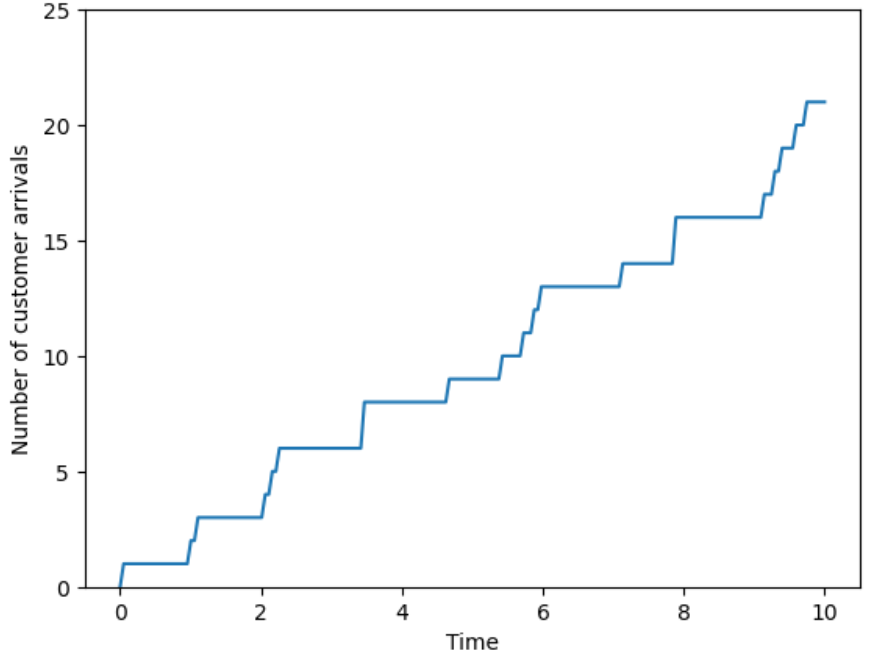
\includegraphics[width=2.91in,height=\textheight,keepaspectratio]{_graphics/PP-outcome-single.png}

}

\caption{\label{fig-PP-rv}A sample outcome for
Example~\ref{exm-PP-outcome}.}

\end{figure}%

\begin{tcolorbox}[enhanced jigsaw, opacityback=0, rightrule=.15mm, coltitle=black, colframe=quarto-callout-tip-color-frame, toprule=.15mm, colbacktitle=quarto-callout-tip-color!10!white, opacitybacktitle=0.6, left=2mm, toptitle=1mm, breakable, title={Solution (click to expand)}, bottomtitle=1mm, colback=white, leftrule=.75mm, titlerule=0mm, arc=.35mm, bottomrule=.15mm]

\begin{refsolution}
Let \(\omega\) denote the outcome represented by Figure~\ref{fig-PP-rv}.

\begin{enumerate}
\def\labelenumi{\arabic{enumi}.}
\tightlist
\item
  The random variable \(N_4\) counts the number of customers who have
  arrived by time 4. \(N_4\) is a discrete random variable taking values
  in the countable set \(\{0, 1, 2, \ldots \}\). To compute the value of
  \(N_4\) for the outcome \(\omega\) in Figure~\ref{fig-PP-rv}, find
  time \(t=4\) on the horizontal axis and find the corresponding value
  on the vertical axis: \(N_4(\omega)=8\) customers; for this outcome,
  the number of customers that have arrived by time 4 is 8.
\item
  The random variable \(N_{6.5}\) which counts the number of customers
  who have arrived by time 6.5 is a discrete random variable taking
  values in the countable set \(\{0, 1, 2, \ldots \}\).
  \(N_{6.5}(\omega)=13\) customers; the number of customers that have
  arrived by time 6.5 is 13. The number of customers is a whole number,
  but time is measured continuously (e.g., 6.5 minutes after opening).
  There is a different discrete random variable \(N_t\) corresponding to
  each value of time \(t\ge 0\), but the possible values of each of
  these variables are \(\{0, 1, 2, \ldots\}\).
\item
  The random variable \(T_4\), which measures the time at which the
  fourth customer arrives, is a continuous random variable (since we're
  assuming time is measured continuously). The smallest possible value
  of \(T_4\) is 0, but there is no definite largest possible value of
  \(T_4\), so \(T_4\) can take theoretically take any value in the
  continuous time interval \([0, \infty)\). The fourth customer arrives
  when the path jumps from 3 customers so far to 4. For the outcome
  \(\omega\) in Figure~\ref{fig-PP-rv} the path jumps from 3 to 4 a
  little after time 2 so \(T_4(\omega)\approx 2.1\) minutes after noon.
\item
  The random variable \(T_5\) which measures the arrival time of the
  fifth customer is a continuous random variable taking values in
  \([0, \infty)\). The fifth customer arrives when the path jumps from 4
  customers so far to 5. For this outcome the path jumps from 4 to 5
  almost right after it jumps from 3 to 4, and almost right after time
  2, so \(T_5(\omega)\approx 2.2\) minutes after noon. There is a
  different continuous random variable \(T_j\) for each customer
  \(j=1, 2, \ldots\), but the possible values of each of these random
  variables is \([0,\infty)\).
\item
  \(W_1\) is the waiting time from open until the first customer
  arrives, a continuous random variable taking values in
  \([0, \infty)\). For the outcome \(\omega\) in Figure~\ref{fig-PP-rv}
  the path jumps from 0 to 1 a little after time 0 so
  \(W_1(\omega)\approx 0.1\) minutes.
\item
  \(W_5\) is the time elapsed between the arrival of the fourth customer
  (at roughly time 2.1 for outcome \(\omega\)) and fifth customer (at
  roughly time 2.2 for outcome \(\omega\)), which is about 0.1 minutes.
\end{enumerate}

\label{sol-PP-rv}

\end{refsolution}

\end{tcolorbox}

\subsection{A random variable is a function}\label{sec-rv-function}

Recall that for a mathematical function\footnote{Throughout, we use
  \(g\) to denote a generic function, and reserve \(f\) to represent a
  probability density function (which we will encounter later).
  Likewise, we represent a generic function argument (or ``dummy
  variable'') with \(u\), since \(x\) is often used to represent
  possible values of a random variable \(X\). In the context of a random
  variable, \(x\) typically represents the \emph{output} of the function
  \(X\) rather than the input (which is a sample space outcome
  \(\omega\).)} \(g\), given an input \(u\), the function returns a real
number \(g(u)\). For example, if \(g\) is the square root function,
\(g(u) = \sqrt{u}\), then \(g(9) = 3\) and \(g(10) = 3.162278...\). If
the input comes from some set \(S\) (i.e.~\(u\in S\)), we write
\(g:S\mapsto \mathbb{R}\).

A random variable \(X\) is a function which maps each outcome \(\omega\)
in the sample space \(\Omega\) to a real number \(X(\omega)\);
\(X:\Omega\mapsto\mathbb{R}\). For a single outcome \(\omega\), the
value \(x = X(\omega)\) is a single number; notice that \(x\) represents
the \emph{output} of the function \(X\) rather than the input. However,
it is important to remember that the random variable \(X\) itself is a
\emph{function}, and \emph{not} a single number.

You are probably familiar with functions expressed as simple closed form
formulas of their inputs: \(g(u)=5u\), \(g(u)=u^2\), \(g(u)=\log u\),
etc. While any random variable is some function, the function is rarely
specified as an explicit mathematical formula of its input \(\omega\).
Often, outcomes are not even numbers (e.g., sequences of coin flips), or
only vaguely specified if at all (e.g., tomorrow's weather conditions).
In Example~\ref{exm-dice-rv} we defined \(X\) through the words ``sum of
two rolls of a fair four-sided dice'' instead of as a
formula\footnote{In Example~\ref{exm-dice-rv} sample space outcomes are
  pairs of rolls. If we denote a generic outcome as
  \(\omega = (\omega_1, \omega_2)\) then
  \(X(\omega) = X((\omega_1, \omega_2)) = \omega_1 + \omega_1\).
  Similarly,
  \(Y(\omega) = Y((\omega_1, \omega_2)) = \max(\omega_1, \omega_2)\).
  But we don't need this level of technical detail; defining \(X\) and
  \(Y\) in words is sufficient.}.

It is more appropriate to think of a random variable as a function in
the sense of a scale at a grocery store which maps a fruit to its
weight, \(X: \text{fruit}\mapsto\text{weight}\). Put an apple on the
scale and the scale returns a number, \(X(\text{apple})\), the weight of
the apple. Likewise, \(X(\text{orange})\), \(X(\text{banana})\). The
random variable \(X\) is the scale itself. This simplistic analogy
assumes a sample space outcome is a single fruit. Of course, it's even
more complicated in reality since an outcome can be considered a set of
fruits, so that we have for example
\(X(\{\text{2 apples}, \text{3 oranges}\})\), and all fruits do not
weigh the same, so that \(X(\text{this apple})\) is not the same as
\(X(\text{that apple})\). But the idea is that a function is like a
scale, with an input (fruits) and an output (weight). The input does not
have to be a number, but the output does.

Suppose I'm going to randomly select some fruits, put them in a brown
grocery bag, and place it on the scale. It wouldn't be feasible to
enumerate all the combinations of fruits I could put in the bag, but
even so you know that any possible combination has some weight which
could be measured by the scale. There is still a function (scale) that
maps an input (fruits in the bag) to a numerical output (weight), even
if that function is not explicitly specified with a mathematical
formula. Now suppose I've selected some fruits and put the bag on the
scale. Even if you can't see what fruits are inside the bag, you can
still read the weight off the scale. But even if you only observe the
weight, you know there was still a background random process of putting
fruits in a bag which resulted in a particular outcome having the
observed weight.

The ``weighing fruits in a bag'' scenario in the previous paragraph
illustrates how probability usually works:

\begin{itemize}
\tightlist
\item
  We typically don't explicitly specify outcomes or the sample space,
  but we know that different outcomes can result in different values of
  random variables. That is, we know there is some function which maps
  outcomes of the random phenomenon to values of the random variable,
  even if we don't have an explicit formula for the inputs to the
  function (sample space outcomes) or the function itself.
\item
  We might not observe outcomes in full detail (e.g., tomorrow's weather
  conditions), but we often can still observe values of random variables
  (e.g., tomorrow's high temperature).
\end{itemize}

\begin{tcolorbox}[enhanced jigsaw, opacityback=0, left=2mm, colframe=quarto-callout-note-color-frame, toprule=.15mm, breakable, colback=white, leftrule=.75mm, arc=.35mm, rightrule=.15mm, bottomrule=.15mm]

\begin{example}[]\protect\hypertarget{exm-meeting-rv-function}{}\label{exm-meeting-rv-function}

Recall the sample space from Example~\ref{exm-meeting-outcome}. Let
\(R\) be the random variable representing Regina's arrival time, and
\(Y\) for Cady.

\begin{enumerate}
\def\labelenumi{\arabic{enumi}.}
\tightlist
\item
  Identify the function that defines \(R\), and the possible values of
  \(R\). (Hint: remember the sample space.)
\item
  Identify the function that defines \(Y\), and the possible values of
  \(Y\).
\end{enumerate}

\end{example}

\end{tcolorbox}

\begin{tcolorbox}[enhanced jigsaw, opacityback=0, rightrule=.15mm, coltitle=black, colframe=quarto-callout-tip-color-frame, toprule=.15mm, colbacktitle=quarto-callout-tip-color!10!white, opacitybacktitle=0.6, left=2mm, toptitle=1mm, breakable, title={Solution (click to expand)}, bottomtitle=1mm, colback=white, leftrule=.75mm, titlerule=0mm, arc=.35mm, bottomrule=.15mm]

\begin{refsolution}
\leavevmode

\begin{enumerate}
\def\labelenumi{\arabic{enumi}.}
\tightlist
\item
  Recall that an outcome is an ordered pair representing the arrival
  times of (Regina, Cady); we can write an outcome as
  \(\omega\equiv(\omega_1, \omega_2)\). Remember there is a single
  sample space corresponding to the pairs of arrival times, rather than
  a separate sample space for each. Therefore, random variables need to
  be defined on this single sample space; inputs to random variables
  defined on this sample space are pairs of arrival times. Regina's
  arrival time is defined by the function
  \(R(\omega) \equiv R((\omega_1, \omega_2))=\omega_1\). That is, \(R\)
  maps the ordered pair \((\omega_1, \omega_2)\) to its first coordinate
  \(\omega_1\). For example, \(R((45, 30.2)) = 45\).
\item
  On this sample space, Cady's arrival time is defined by the function
  \(Y(\omega) \equiv Y((\omega_1, \omega_2))=\omega_2\). That is, \(Y\)
  maps the ordered pair to its second coordinate. The input to \(Y\) is
  a pair of numbers (Regina, Cady) and the output is Cady's arrival time
  only. For example, \(Y((45, 30.2)) = 30.2\).
\end{enumerate}

\label{sol-exm-meeting-rv-function}

\end{refsolution}

\end{tcolorbox}

\subsection{Tranformations of random
variables}\label{tranformations-of-random-variables}

We are often interested in random variables that are derived from
others. For example, if the random variable \(X\) represents the radius
(cm) of a randomly selected circle, then \(Y = \pi X^2\) is a random
variable representing the circle's area (\(\text{cm}^2\)). If the random
variables \(W\) and \(T\) represent the weight (kg) and height (m),
respectively, of a randomly selected person, then \(S = W / T^2\) is a
random variable representing the person's body mass index
(\(\text{kg}/\text{m}^2\)).

A function of a random variable is also a random variable. That is, if
\(X\) is a random variable and \(g\) is a function, then \(Y=g(X)\) is
also a random variable\footnote{\(Y(\omega) = g(X(\omega))\) so \(Y\)
  maps \(\Omega\) to \(\mathbb{R}\) via the \emph{composition} of the
  functions \(g\) and \(X\); that is, \(Y=g\circ X\) where
  \((g\circ X):\Omega\mapsto \mathbb{R}\)}. For example, if \(u\) is a
radius of a circle, the function \(g(u) = \pi u^2\) outputs its area; if
\(X\) is a random variable representing the radius of a randomly
selected circle then \(Y = g(X)=\pi X^2\) is a random variable
representing the circle's area.

Sums and products, etc., of random variables \emph{defined on the same
sample space} are random variables. That is, if random variables \(X\)
and \(Y\) are defined on the same sample space then \(X+Y\), \(X-Y\),
\(XY\), and \(X/Y\) are also random variables. Similarly, it is possible
to make comparisons such as \(X\ge Y\) and apply other transformations
for random variables defined on the same sample space.

\begin{tcolorbox}[enhanced jigsaw, opacityback=0, left=2mm, colframe=quarto-callout-note-color-frame, toprule=.15mm, breakable, colback=white, leftrule=.75mm, arc=.35mm, rightrule=.15mm, bottomrule=.15mm]

\begin{example}[]\protect\hypertarget{exm-rv-transform-simple}{}\label{exm-rv-transform-simple}

Continuning Example~\ref{exm-simple-event}. In basketball games, teams
attempt field goals and they score points for made field goals. Made
field goals are worth either 2 or 3 points. Teams also attempt free
throws which are worth 1 point if made. Each team plays 82 games in a
season.

For the team that wins the top pick in the lottery in the 2022-2023
season, let

\begin{itemize}
\tightlist
\item
  \(W\) be the number of wins
\item
  \(Y_1\) be free throw attempts per game (FT)
\item
  \(Y_2\) be 2 point field goal attempts per game (FG2)
\item
  \(Y_3\) be 3 point field goal attempts per game (FG3)
\item
  \(X_1\) be free throws made per game (FTA)
\item
  \(X_2\) be 2 point field goals made per game (FG2A)
\item
  \(X_3\) be 3 point field goals made per game (FG3A)
\end{itemize}

Interpret the following random variables in this context. How could they
be represented in a table like Table~\ref{tbl-nba-draft}?

\begin{enumerate}
\def\labelenumi{\arabic{enumi}.}
\tightlist
\item
  \(82 - W\)
\item
  \(W / 82\)
\item
  \(X_1 / Y_1\)
\item
  \(\frac{X_2 + X_3}{Y_2+Y_3}\)
\item
  \(\frac{Y_3}{Y_2+Y_3}\)
\item
  \(3X_3 + 2X_2 + X_1\)
\end{enumerate}

\end{example}

\end{tcolorbox}

\begin{tcolorbox}[enhanced jigsaw, opacityback=0, rightrule=.15mm, coltitle=black, colframe=quarto-callout-tip-color-frame, toprule=.15mm, colbacktitle=quarto-callout-tip-color!10!white, opacitybacktitle=0.6, left=2mm, toptitle=1mm, breakable, title={Solution (click to expand)}, bottomtitle=1mm, colback=white, leftrule=.75mm, titlerule=0mm, arc=.35mm, bottomrule=.15mm]

\begin{refsolution}
Table~\ref{tbl-nba-draft-transform} provides a representation of these
random variables. For the team that wins the 2023 NBA draft in the
2022-2023 season:

\begin{enumerate}
\def\labelenumi{\arabic{enumi}.}
\tightlist
\item
  \(82 - W\) is the team's number of losses
\item
  \(W / 82\) is the proportion of games in the season that the team won
  (a.k.a., winning percentage, as a decimal)
\item
  \(X_1 / Y_1\) is the proportion of free throw attempts that the team
  successfully made (a.k.a., free throw percentage, as a decimal)
\item
  \(\frac{X_2 + X_3}{Y_2+Y_3}\) is the proportion of total field goal
  attempts that the team successfully made (a.k.a., field goal
  percentage, as a decimal)
\item
  \(\frac{Y_3}{Y_2+Y_3}\) is the proportion of the team's total field
  goal attempts that were 3 point attempts
\item
  \(3X_3 + 2X_2 + X_1\) is the total points per game scored by the team
  (any differences between Table~\ref{tbl-nba-draft-transform} and PPG
  in Table~\ref{tbl-nba-draft} are due to rounding.)
\end{enumerate}

\label{sol-rv-transform-simple}

\end{refsolution}

\end{tcolorbox}

\begin{table}

\caption{\label{tbl-nba-draft-transform}The random variables from
Example~\ref{exm-rv-transform-simple} for teams in the 2023 NBA Draft
Lottery.}

\centering{

\centering
\begin{tabular}[t]{l|r|r|r|r|r|r|r|r|r|r|r|r|r}
\hline
Team & $W$ & $X_3$ & $Y_3$ & $X_2$ & $Y_2$ & $X_1$ & $Y_1$ & $82-W$ & $W/82$ & $X_1/Y_1$ & $\frac{X_2+X_3}{Y_2+Y_3}$ & $\frac{Y_3}{Y_2+Y_3}$ & $3X_3 + 2X_2 + X_1$\\
\hline
Detroit Pistons & 17 & 11.4 & 32.4 & 28.2 & 54.6 & 19.8 & 25.7 & 65 & 0.207 & 0.770 & 0.455 & 0.372 & 110.4\\
\hline
Houston Rockets & 22 & 10.4 & 31.9 & 30.2 & 56.9 & 19.1 & 25.3 & 60 & 0.268 & 0.755 & 0.457 & 0.359 & 110.7\\
\hline
San Antonio Spurs & 22 & 11.1 & 32.2 & 32.0 & 60.4 & 15.8 & 21.2 & 60 & 0.268 & 0.745 & 0.465 & 0.348 & 113.1\\
\hline
Charlotte Hornets & 27 & 10.7 & 32.5 & 30.5 & 57.9 & 17.6 & 23.6 & 55 & 0.329 & 0.746 & 0.456 & 0.360 & 110.7\\
\hline
Portland Trail Blazers & 33 & 12.9 & 35.3 & 27.6 & 50.1 & 19.6 & 24.6 & 49 & 0.402 & 0.797 & 0.474 & 0.413 & 113.5\\
\hline
Orlando Magic & 34 & 10.8 & 31.1 & 29.8 & 55.2 & 19.6 & 25.0 & 48 & 0.415 & 0.784 & 0.470 & 0.360 & 111.6\\
\hline
Indiana Pacers & 35 & 13.6 & 37.0 & 28.4 & 52.6 & 18.7 & 23.7 & 47 & 0.427 & 0.789 & 0.469 & 0.413 & 116.3\\
\hline
Washington Wizards & 35 & 11.3 & 31.7 & 30.9 & 55.2 & 17.6 & 22.4 & 47 & 0.427 & 0.786 & 0.486 & 0.365 & 113.3\\
\hline
Utah Jazz & 37 & 13.3 & 37.8 & 29.2 & 52.0 & 18.7 & 23.8 & 45 & 0.451 & 0.786 & 0.473 & 0.421 & 117.0\\
\hline
Dallas Mavericks & 38 & 15.2 & 41.0 & 24.8 & 43.3 & 19.0 & 25.1 & 44 & 0.463 & 0.757 & 0.474 & 0.486 & 114.2\\
\hline
Chicago Bulls & 40 & 10.4 & 28.9 & 32.1 & 57.9 & 17.6 & 21.8 & 42 & 0.488 & 0.807 & 0.490 & 0.333 & 113.0\\
\hline
Oklahoma City Thunder & 40 & 12.1 & 34.1 & 31.0 & 58.5 & 19.2 & 23.7 & 42 & 0.488 & 0.810 & 0.465 & 0.368 & 117.5\\
\hline
Toronto Raptors & 41 & 10.7 & 32.0 & 31.1 & 59.3 & 18.4 & 23.4 & 41 & 0.500 & 0.786 & 0.458 & 0.350 & 112.7\\
\hline
New Orleans Pelicans & 42 & 11.0 & 30.1 & 31.1 & 57.5 & 19.3 & 24.4 & 40 & 0.512 & 0.791 & 0.481 & 0.344 & 114.5\\
\hline
\end{tabular}

}

\end{table}%

Remember that we can visualize outcomes as rows in a spreadsheet with
random variables as columns. Random variables defined on the same sample
space can be put in a single spreadsheet. Each row corresponds to an
outcome, and reading across any row there is a value in the column
corresponding to each random variable. Random variables derived from
transformations of other random variables append columns to the
spreadsheet. New random variables can be defined by going row-by-row,
outcome-by-outcome, and applying a transformation within each row to the
values of other random variables.

Using capital letters like \(X\) or \(Y\) to denote random variables is
standard practice. To help develop comfort with this mathematical
notation, we will often label columns in tables with their random
variable symbols (as we did in Table~\ref{tbl-nba-draft-transform}).
Later, when writing code we will often denote random variables with
symbols like \texttt{X} or \texttt{Y}. However, keep in mind that
mathematical symbols like \(X\) or \(Y\) represent variables in a
context. While you should develop comfort with the notation, you
can---and probably should---use more informative labels like ``wins'' or
\texttt{wins} rather than \(W\).

\begin{tcolorbox}[enhanced jigsaw, opacityback=0, left=2mm, colframe=quarto-callout-note-color-frame, toprule=.15mm, breakable, colback=white, leftrule=.75mm, arc=.35mm, rightrule=.15mm, bottomrule=.15mm]

\begin{example}[]\protect\hypertarget{exm-meeting-rv}{}\label{exm-meeting-rv}

Continuing Example~\ref{exm-meeting-rv-function}.

\begin{enumerate}
\def\labelenumi{\arabic{enumi}.}
\tightlist
\item
  What does the random variable \(U_1 = R / 60\) represent in context?
  What are the possible values of \(U_1\)?
\item
  What does the random variable \(T = \min(R, Y)\) represent in context?
  What are the possible values of \(T\)?
\item
  What does the random variable \(W = |R - Y|\) represent in context?
  What are the possible values of \(W\)?
\end{enumerate}

\end{example}

\end{tcolorbox}

\begin{tcolorbox}[enhanced jigsaw, opacityback=0, rightrule=.15mm, coltitle=black, colframe=quarto-callout-tip-color-frame, toprule=.15mm, colbacktitle=quarto-callout-tip-color!10!white, opacitybacktitle=0.6, left=2mm, toptitle=1mm, breakable, title={Solution (click to expand)}, bottomtitle=1mm, colback=white, leftrule=.75mm, titlerule=0mm, arc=.35mm, bottomrule=.15mm]

\begin{refsolution}
\leavevmode

\begin{enumerate}
\def\labelenumi{\arabic{enumi}.}
\tightlist
\item
  \(U_1= R / 60\) represents Regina's arrival time measured as a
  fraction of the hour after noon. For example, if Regina arrives 15
  minutes after noon then \(R=15\) and \(U_1= 15/60 = 0.25\). \(U_1\)
  takes values in {[}0, 1{]}.
\item
  \(T=\min(R, Y)\) represents the time (minutes after noon) of the first
  arrival. For example, if Regina arrives 15 minutes after noon and Cady
  22.3 minutes after noon then \(R=15\), \(C=22.3\) and
  \(T=\min(15, 22.3) = 15\). \(T\) takes values in \([0, 60]\). If
  either Regina and Cady arrives at time 0 (noon) then \(T\) is 0, the
  smallest possible value of \(T\); if both arrive at 1:00 then \(T\) is
  60, the largest possible value of \(T\).
\item
  \(W=|R-Y|\) represents the amount of time the first person to arrive
  waits for the second person to arrive. For example, if Regina arrives
  15 minutes after noon and Cady 22.3 minutes after noon then \(R=15\),
  \(C=22\) and \(W = |15-22.3| = 7.3\). \(W\) takes values in
  \([0, 60]\). If both Regina and Cady arrive at the same time then
  \(W\) is 0; if one arrives at noon and the other at 1:00 then \(W\) is
  60, the largest possible value of \(W\).
\end{enumerate}

\label{sol-meeting-rv}

\end{refsolution}

\end{tcolorbox}

\subsection{Indicator random variables}\label{sec-indicator-rv}

Random variables that only take two possible values, 0 and 1, have a
special name.

\begin{definition}[]\protect\hypertarget{def-indicator}{}\label{def-indicator}

An \textbf{indicator (a.k.a., Bernoulli, a.k.a.
Boolean)}\index{indicator} random variable can take only the values 0 or
1. If \(A\) is an event then the corresponding indicator random variable
\(\textrm{I}_A\) is defined as \[
\textrm{I}_A(\omega) =
\begin{cases}
1, & \omega \in A,\\
0, & \omega \notin A
\end{cases}
\] That is, \(\textrm{I}_A\) equals 1 if event \(A\) occurs, and
\(\textrm{I}_A\) equals 0 if event \(A\) does not occur.

\end{definition}

Indicators provide the bridge between events (sets) and random variables
(functions). Any event either occurs or not; a realization of any event
is either true (\(\omega \in A\)) or false (\(\omega \notin A\)). An
indicator random variable just translates ``true'' or ``false'' into
numbers, 1 for ``true'' and 0 for ``false''.

\begin{tcolorbox}[enhanced jigsaw, opacityback=0, left=2mm, colframe=quarto-callout-note-color-frame, toprule=.15mm, breakable, colback=white, leftrule=.75mm, arc=.35mm, rightrule=.15mm, bottomrule=.15mm]

\begin{example}[]\protect\hypertarget{exm-matching-indicator}{}\label{exm-matching-indicator}

Recall the sample space from Example~\ref{exm-matching-outcome} for the
matching problem with \(n=4\). Let the random variable \(X\) count the
number of objects that are placed in the correct spot. Let \(I_1\) be
equal to 1 if object 1 is placed (correctly) in spot 1, and define
\(I_2, I_3, I_4\) similarly.

\begin{enumerate}
\def\labelenumi{\arabic{enumi}.}
\tightlist
\item
  Construct a table identifying the value of \(X, I_1, \ldots, I_4\) for
  each outcome in the sample space.
\item
  Identify the possible values of \(X\).
\item
  What is the relationship between \(I_3\) and event \(A_3\) from
  Example~\ref{exm-matching-event}?
\item
  How can you express \(X\) in terms of \(I_1, \ldots, I_4\)?
\end{enumerate}

\end{example}

\end{tcolorbox}

\begin{tcolorbox}[enhanced jigsaw, opacityback=0, rightrule=.15mm, coltitle=black, colframe=quarto-callout-tip-color-frame, toprule=.15mm, colbacktitle=quarto-callout-tip-color!10!white, opacitybacktitle=0.6, left=2mm, toptitle=1mm, breakable, title={Solution (click to expand)}, bottomtitle=1mm, colback=white, leftrule=.75mm, titlerule=0mm, arc=.35mm, bottomrule=.15mm]

\begin{refsolution}
\leavevmode

\begin{enumerate}
\def\labelenumi{\arabic{enumi}.}
\tightlist
\item
  See Table~\ref{tbl-matching-indicator-tab}. Each random variable
  corresponds to a different column in the table.
\item
  \(X\) can take values 0, 1, 2, and 4, but 3 is not a possible value of
  \(X\).
\item
  \(I_3\) is equal to 1 only for outcomes that satisfy \(A_3\), the
  event that object 3 is placed in spot 3; \(I_3\) is equal 0 for
  outcomes that do not satisfy event \(A_3\). In this way, the value of
  the random variable \(I_3\) indicates whether or not the event \(A_3\)
  occurs; that is, \(I_3\) is the indicator random variable of event
  \(A_3\), \(I_3 = \textrm{I}_{A_3}\).
\item
  For every outcome (row), the value of \(X\) is equal to the sum of the
  values of \(I_1\), \(I_2\), \(I_3\), \(I_4\). That is,
  \(X = I_1+I_2+I_3+I_4\). For example, for outcome 2134, \(X\) is equal
  to 2, \(I_1\) and \(I_2\) are equal to 0, and \(I_3\) and \(I_4\) are
  equal to 1, and \(2 = 0 + 0 + 1 + 1\). The relationship
  \(X = I_1+I_2+I_3+I_4\) is true for every outcome (row). The
  spot-by-spot indicators provide a way to incrementally count the total
  number of matches.
\end{enumerate}

\label{sol-matching-indicator}

\end{refsolution}

\end{tcolorbox}

\begin{table}

\caption{\label{tbl-matching-indicator-tab}Total number of matches and
indicator random variables for each item in the matching problem with
\(n=4\).}

\centering{

\centering
\begin{tabular}[t]{lrrrrr}
\toprule
Outcome & $X$ & $I_1$ & $I_2$ & $I_3$ & $I_4$\\
\midrule
1234 & 4 & 1 & 1 & 1 & 1\\
1243 & 2 & 1 & 1 & 0 & 0\\
1324 & 2 & 1 & 0 & 0 & 1\\
1342 & 1 & 1 & 0 & 0 & 0\\
1423 & 1 & 1 & 0 & 0 & 0\\
\addlinespace
1432 & 2 & 1 & 0 & 1 & 0\\
2134 & 2 & 0 & 0 & 1 & 1\\
2143 & 0 & 0 & 0 & 0 & 0\\
2314 & 1 & 0 & 0 & 0 & 1\\
2341 & 0 & 0 & 0 & 0 & 0\\
\addlinespace
2413 & 0 & 0 & 0 & 0 & 0\\
2431 & 1 & 0 & 0 & 1 & 0\\
3124 & 1 & 0 & 0 & 0 & 1\\
3142 & 0 & 0 & 0 & 0 & 0\\
3214 & 2 & 0 & 1 & 0 & 1\\
\addlinespace
3241 & 1 & 0 & 1 & 0 & 0\\
3412 & 0 & 0 & 0 & 0 & 0\\
3421 & 0 & 0 & 0 & 0 & 0\\
4123 & 0 & 0 & 0 & 0 & 0\\
4132 & 1 & 0 & 0 & 1 & 0\\
\addlinespace
4213 & 1 & 0 & 1 & 0 & 0\\
4231 & 2 & 0 & 1 & 1 & 0\\
4312 & 0 & 0 & 0 & 0 & 0\\
4321 & 0 & 0 & 0 & 0 & 0\\
\bottomrule
\end{tabular}

}

\end{table}%

Even though they seem simple, indicator random variables are very
useful. In the matching problem, it is not feasible to enumerate the
outcomes and count when there is a large number \(n\) of items and
spots. Using indicators allows you to count incrementally---is just this
item in the correct spot?--- rather than all at once. Representing a
count as a sum of indicator random variables is a very common and useful
strategy, especially in problems that involve ``find the expected number
of\ldots{}''

Here is a little story that illustrates the idea of incremental counting
with indicators. Imagine a dad and his young child are reading a picture
book. They come to a page that has twenty pictures of fruits, of which
seven are bananas. The following conversation ensues.

\begin{itemize}
\tightlist
\item
  Dad: Can you count all the bananas? Let's see! How many bananas have
  we counted so far?
\item
  Kid: We haven't started counting yet!
\item
  Dad: Right, so how many bananas have we counted so far?
\item
  Kid: Zero.
\item
  Dad: That's right! We've counted zero bananas so far. (Dad points to a
  banana.) Is that a banana?
\item
  Kid: Yes!
\item
  Dad: So how many more bananas did we just count?
\item
  Kid: One more.
\item
  Dad: So how many bananas have we counted so far?
\item
  Kid: One.
\item
  Dad: Great job! We've counted one banana so far. (Dad points to a
  different banana.) Is that a banana?
\item
  Kid: Yes!
\item
  Dad: So how many more bananas did we just count?
\item
  Kid: We counted one more banana.
\item
  Dad: So how many bananas have we counted so far?
\item
  Kid: Two.
\item
  Dad: Great job! We've counted two bananas so far. (Dad points to a
  different banana.) Is that a banana?
\item
  Kid: Yes!
\item
  Dad: So how many more bananas did we just count?
\item
  Kid: We counted one more banana.
\item
  Dad: So how many bananas have we counted so far?
\item
  Kid: Three.
\item
  Dad: Great job! We've counted three bananas so far. (Dad points to an
  orange\footnote{Orange you glad I didn't say banana?}.) Is that a
  banana?
\item
  Kid: No, that's an orange!
\item
  Dad: So how many more bananas did we just count?
\item
  Kid: Zero. It was not a banana!
\item
  Dad: So how many bananas have we counted so far?
\item
  Kid: Still three.
\item
  Dad: Great job! We've counted three bananas so far. (Continues in this
  manner until Dad points to the twentieth and last fruit on the page, a
  banana.) Almost done. We've counted six bananas so far. Is that a
  banana?
\item
  Kid: Yes!
\item
  Dad: So how many more bananas did we just count?
\item
  Kid: We counted one more banana.
\item
  Dad: So how many bananas have we counted so far?
\item
  Kid: Seven.
\item
  Dad: We looked at each fruit on the page. How many were bananas?
\item
  Kid: Seven.
\item
  Dad: Great job! Now you know how indicator random variables can be
  used to count.
\end{itemize}

In the story, the kid counted the bananas by examining each object,
determining whether or not it was a banana, and then incrementing the
banana counter by 1 for each object that was a banana (and by 0 for the
objects that were not bananas). The kid essentially created an indicator
(of ``banana'') variable for each object on the page (\(I_{B_1}=1\),
\(I_{B_2}=1\), \(I_{B_3}=1\), \(I_{B_4}=0\ldots\), \(I_{B_{20}}=1\)) and
then summed these indicators to obtain the total count of bananas. This
strategy gives a way of breaking down a complicated counting problem
into smaller pieces and counting incrementally.

\begin{tcolorbox}[enhanced jigsaw, opacityback=0, left=2mm, colframe=quarto-callout-note-color-frame, toprule=.15mm, breakable, colback=white, leftrule=.75mm, arc=.35mm, rightrule=.15mm, bottomrule=.15mm]

\begin{example}[]\protect\hypertarget{exm-matching-indicator-properties}{}\label{exm-matching-indicator-properties}

Continuing Example~\ref{exm-matching-indicator}, interpret each of the
following random variables.

\begin{enumerate}
\def\labelenumi{\arabic{enumi}.}
\tightlist
\item
  \(1 - \textrm{I}_3\)
\item
  \(\textrm{I}_1 \textrm{I}_2\), that is, the product of
  \(\textrm{I}_1\) and \(\textrm{I}_2\)
\item
  \(\textrm{I}_1 + \textrm{I}_2 - \textrm{I}_1 \textrm{I}_2\).
\end{enumerate}

\end{example}

\end{tcolorbox}

\begin{tcolorbox}[enhanced jigsaw, opacityback=0, rightrule=.15mm, coltitle=black, colframe=quarto-callout-tip-color-frame, toprule=.15mm, colbacktitle=quarto-callout-tip-color!10!white, opacitybacktitle=0.6, left=2mm, toptitle=1mm, breakable, title={Solution (click to expand)}, bottomtitle=1mm, colback=white, leftrule=.75mm, titlerule=0mm, arc=.35mm, bottomrule=.15mm]

\begin{refsolution}
\leavevmode

\begin{enumerate}
\def\labelenumi{\arabic{enumi}.}
\tightlist
\item
  \(1 - \textrm{I}_3\) is 1 if \(\textrm{I}_3 = 0\), which occurs when
  object 3 is \emph{not} in spot 3, and \(1 - \textrm{I}_3\) is 0
  otherwise. So \(1 - \textrm{I}_3\) is the indicator that object 3 is
  \emph{not} placed in spot 3; \(1-\textrm{I}_3 = \textrm{I}_{A_3^c}\).
\item
  \(\textrm{I}_1 \textrm{I}_2\) is 1 if both \(\textrm{I}_1\) and
  \(\textrm{I}_2\) are 1, which occurs when objects 1 and 2 are in the
  correct spots; otherwise, \(\textrm{I}_1 \textrm{I}_2\) is 0.
  Therefore \(\textrm{I}_1 \textrm{I}_2\) is the indicator that object 1
  is placed in spot 1 \emph{and} object 2 is placed in spot 2;
  \(\textrm{I}_1\textrm{I}_2 = \textrm{I}_{A_1 \cap A_2}\).
\item
  \(\textrm{I}_1 + \textrm{I}_2 - \textrm{I}_1 \textrm{I}_2\) is 1 if:
  object 1 is in spot 1 but object 2 is not in spot 2 (1 + 0 - 0),
  object 1 is not in spot 1 but object 2 is in spot 2 (0 + 1 - 0), or if
  both object 1 is in spot 1 and object 2 is in spot 2 (1 + 1 - 1).
  \(\textrm{I}_1 + \textrm{I}_2 - \textrm{I}_1 \textrm{I}_2\) is 0 only
  if object 1 is not in spot 1 and object 2 is not in spot 2. Therefore
  \(\textrm{I}_1 + \textrm{I}_2 - \textrm{I}_1 \textrm{I}_2\) is the
  indicator that object 1 is placed in spot 1 \emph{or} object 2 is
  placed in spot 2;
  \(\textrm{I}_1 + \textrm{I}_2 - \textrm{I}_1 \textrm{I}_2 = \textrm{I}_{A_1 \cup A_2}\).
\end{enumerate}

\label{sol-matching-indicator-properties}

\end{refsolution}

\end{tcolorbox}

Example~\ref{exm-matching-indicator-properties} illustrates that for two
events \(A\) and \(B\) \begin{align*}
\textrm{I}_{A^c} & = 1 - \textrm{I}_A & & \\
\textrm{I}_{A \cap B} & = \textrm{I}_A \textrm{I}_B & & =\min(\textrm{I}_A, \textrm{I}_B)\\
\textrm{I}_{A \cup B} & = \textrm{I}_A + \textrm{I}_B - \textrm{I}_{A \cap B} & & = \max(I_A, I_B)
\end{align*}

In particular, the indicator of an intersection is the product of the
indicators of each event. The \(\min, \max\), and product formulas work
for more than two events, but the addition formula is more
complicated\footnote{See the
  \href{https://mathworld.wolfram.com/Inclusion-ExclusionPrinciple.html}{inclusion-exclusion
  principle}}.

\subsection{Events involving random
variables}\label{events-involving-random-variables}

Many events of interest involve random variables. The event ``tomorrow's
high temperature is above 75°F'' involves the random variable
``tomorrow's high temperature''. Each possible outcome of tomorrow's
weather conditions will correspond to a value of high temperature, but
only some of these outcomes will result in values of high temperature
above 75 °F.

\begin{tcolorbox}[enhanced jigsaw, opacityback=0, left=2mm, colframe=quarto-callout-note-color-frame, toprule=.15mm, breakable, colback=white, leftrule=.75mm, arc=.35mm, rightrule=.15mm, bottomrule=.15mm]

\begin{example}[]\protect\hypertarget{exm-rv-event-simple}{}\label{exm-rv-event-simple}

Continuning Example~\ref{exm-simple-event}. For the team that wins the
top pick in the lottery, let

\begin{itemize}
\tightlist
\item
  \(X\) be the number of previous championships won by the team that
  wins the top pick in the lottery
\item
  \(Y\) be the number of wins in the 2022-2023 season
\item
  \(Z\) be the points per game in the 2022-2023 season
\item
  \(I\) be the indicator random variable that the team is in the Western
  Conference
\end{itemize}

Identify and interpret the following events.

\begin{enumerate}
\def\labelenumi{\arabic{enumi}.}
\tightlist
\item
  \(\{I=1\}\)
\item
  \(\{X = 0\}\)
\item
  \(\{Y < 25\}\)
\item
  \(\{Z > 115\}\)
\item
  \(\{I = 1, X = 0\}\)
\item
  \(\{I = 1, X = 0, Y < 25\}\)
\item
  \(\{I = 1\}\cup \{X = 0\}\)
\item
  \(\{X \ge 1\}\)
\end{enumerate}

\end{example}

\end{tcolorbox}

\begin{tcolorbox}[enhanced jigsaw, opacityback=0, rightrule=.15mm, coltitle=black, colframe=quarto-callout-tip-color-frame, toprule=.15mm, colbacktitle=quarto-callout-tip-color!10!white, opacitybacktitle=0.6, left=2mm, toptitle=1mm, breakable, title={Solution (click to expand)}, bottomtitle=1mm, colback=white, leftrule=.75mm, titlerule=0mm, arc=.35mm, bottomrule=.15mm]

\begin{refsolution}
These events are the same as those in Example~\ref{exm-rv-event-simple}
just with different notation.

\begin{enumerate}
\def\labelenumi{\arabic{enumi}.}
\tightlist
\item
  \(\{I = 1\} = \{\text{Houston, San Antonio, Portland, Utah, Dallas, Oklahoma City, New Orleans}\}\)
  is the event that the team is in the Western Conference.
\item
  \(\{X = 0\} = \{\text{Charlotte, Orlando, Indiana, Utah, New Orleans}\}\)
  is the event that the team has never won a championship.
\item
  \(\{Y < 25\} = \{\text{Detroit, Houston, San Antonio}\}\) is the event
  that the team won fewer than 25 games in the 2022-2023 season
\item
  \(\{Z > 115\} = \{\text{Indiana, Utah, Oklahoma City}\}\) is the event
  that the team scored over 115 points per game in the 2022-2023 season
\item
  \(\{I = 1, X = 0\} = \{\text{Utah, New Orleans}\}\) is the event that
  the team is in the Western Conference and has won no previous
  championships.
\item
  \(\{I = 1, X = 0, Y < 25\}=\{\text{Utah}\}\) is the event that the
  team is in the Western Conference, has won no previous championships,
  and scored over 115 points per game in the 2022-2023 season.
\item
  \(\{I = 1\}\cup \{X = 0\}=\{\text{Charlottle, Houston, San Antonio, Portland, Orlando, Indians, Utah, Dallas, Oklahoma City, New Orleans}\}\)
  is the event that the team is in the Western Conference or has won no
  previous championships.
\item
  \(\{X \ge 1\}=\{\text{Detroit, Houston, San Antonio, Portland, Washington, Dallas, Chicago, Oklahoma City, Toronto}\}\)
  is the event that the team has won at least one previous championship.
\end{enumerate}

\label{sol-rv-event-simple}

\end{refsolution}

\end{tcolorbox}

The expressions \(X=x\) or \(\{X=x\}\) are shorthand for the
\emph{event} that the random variable \(X\) takes the value \(x\).
Remember that any event is a collection of outcomes that satisfy some
criteria, a subset of the sample space. So objects like \(\{X=x\}\) are
sets representing the outcomes for which the value of the random
variable \(X\) is equal to the number \(x\). Remember to think of the
capital letter \(X\) as a label standing in for a formula like ``the sum
of two rolls of a four-sided die'' and \(x\) as a dummy variable
standing in for a particular value like 3.

\begin{tcolorbox}[enhanced jigsaw, opacityback=0, left=2mm, colframe=quarto-callout-note-color-frame, toprule=.15mm, breakable, colback=white, leftrule=.75mm, arc=.35mm, rightrule=.15mm, bottomrule=.15mm]

\begin{example}[]\protect\hypertarget{exm-dice-rv-event}{}\label{exm-dice-rv-event}

Roll a four-sided die twice, and record the result of each roll in
sequence. Recall the sample space from Example~\ref{exm-dice-outcome}.
Let \(X\) be the sum of the two dice, and let \(Y\) be the larger of the
two rolls (or the common value if both rolls are the same). Identify and
interpret each of the following.

\begin{enumerate}
\def\labelenumi{\arabic{enumi}.}
\tightlist
\item
  \(\{X = 4\}\).
\item
  \(\{X = 3\}\).
\item
  \(\{X \le 3\}\).
\item
  \(\{Y = 4\}\).
\item
  \(\{Y = 3\}\).
\item
  \(\{Y \le 3\}\).
\item
  \(\{X = 4, Y = 3\}\) (that is, \(\{X = 4\}\cap \{Y = 3\}\)).
\item
  \(\{X = 4, Y \le 3\}\).
\item
  \(\{X = 3, Y = 3\}\).
\end{enumerate}

\end{example}

\end{tcolorbox}

\begin{tcolorbox}[enhanced jigsaw, opacityback=0, rightrule=.15mm, coltitle=black, colframe=quarto-callout-tip-color-frame, toprule=.15mm, colbacktitle=quarto-callout-tip-color!10!white, opacitybacktitle=0.6, left=2mm, toptitle=1mm, breakable, title={Solution (click to expand)}, bottomtitle=1mm, colback=white, leftrule=.75mm, titlerule=0mm, arc=.35mm, bottomrule=.15mm]

\begin{refsolution}
Notice we encountered many of these events in
Example~\ref{exm-dice-event}, but now we are denoting the events in
terms of random variables.

\begin{enumerate}
\def\labelenumi{\arabic{enumi}.}
\tightlist
\item
  \(\{X = 4\}\), which consists of the outcomes (1, 3), (2, 2), (3, 1),
  is the event that the sum of the two dice is 4. Recalling
  Example~\ref{exm-dice-event}, \(A = \{X = 4\}\).
\item
  \(\{X = 3\}\), which consists of outcomes (1, 2) and (2, 1), is the
  event that the sum of the two dice is 3.
\item
  \(\{X \le 3\}\), which consists of outcomes (1, 1), (1, 2), and (2,
  1), is the event that the sum of the two dice is at most 3. Recalling
  Example~\ref{exm-dice-event}, \(B = \{X \le 3\}\).
\item
  \(\{Y = 4\}=\{(1, 4), (2, 4), (3, 4), (4, 4), (4, 1), (4, 2), (4,3)\}\)
  is the event that the larger of the two rolls is 4.
\item
  \(\{Y = 3\}=\{(1, 3), (2, 3), (3, 3), (3, 1), (3, 2)\}\) is the event
  that the larger of the two rolls is 3. Recalling
  Example~\ref{exm-dice-event}, \(C = \{Y = 3\}\).
\item
  \(\{Y \le 3\}=\{(1, 1), (1, 2), (1, 3), (2, 1), (2, 2), (2, 3), (3, 1), (3, 2), (3, 3)\}\)
  is the event that the larger of the two rolls is at most 3. Notice
  that since in this example \(Y\) can only take values 1, 2, 3, 4, we
  have \(\{Y\le 3\} = \{Y=4\}^c\).
\item
  \(\{X = 4, Y = 3\} \equiv \{X = 4\}\cap \{Y = 3\}=\{(1, 3), (3, 1)\}\)
  is the event that both the sum of the two dice is 4 and the larger of
  the two rolls is 3. Even though this involves two random variables, it
  is a single event (that is, a single subset of the sample space).
  There are only two outcomes for which both the sum of the two dice is
  4 and the larger of the two dice is 3.
\item
  \(\{X = 4, Y \le 3\} \equiv \{X = 4\}\cap \{Y \le 3\}=\{(1, 3), (2, 2), (3, 1)\}\)
  is the event that both the sum of the two dice is 4 and the larger of
  the two rolls is at most 3. Notice that since in this example
  \(\{X=4\} \subset \{Y\le 3\}\), we have
  \(\{X = 4, Y \le 3\} = \{X=4\}\). If the sum is 4 we know the larger
  roll must be at most 3.
\item
  \(\{X = 3, Y = 3\} \equiv \{X = 3\}\cap \{Y = 3\}=\emptyset\), since
  there are no outcomes for which both the sum is 3 and the larger of
  the two dice is 3. (If the the larger of the two dice is 3, then the
  sum must be at least 4.)
\end{enumerate}

\label{sol-dice-rvevent}

\end{refsolution}

\end{tcolorbox}

\begin{table}

\caption{\label{tbl-dice-rv-event-sol-table}Table representing the sum
(\(X\)) and larger (\(Y\)) of two rolls of a four-sided die. The event
\(X = 4\) is highlighted in orange.}

\centering{

\centering
\begin{tabular}[t]{lrr}
\toprule
Outcome (First roll, second roll) & X (sum) & Y (max)\\
\midrule
(1, 1) & 2 & 1\\
(1, 2) & 3 & 2\\
\cellcolor[HTML]{FFA500}{\textcolor{white}{\textbf{(1, 3)}}} & \cellcolor[HTML]{FFA500}{\textcolor{white}{\textbf{4}}} & \cellcolor[HTML]{FFA500}{\textcolor{white}{\textbf{3}}}\\
(1, 4) & 5 & 4\\
(2, 1) & 3 & 2\\
\addlinespace
\cellcolor[HTML]{FFA500}{\textcolor{white}{\textbf{(2, 2)}}} & \cellcolor[HTML]{FFA500}{\textcolor{white}{\textbf{4}}} & \cellcolor[HTML]{FFA500}{\textcolor{white}{\textbf{2}}}\\
(2, 3) & 5 & 3\\
(2, 4) & 6 & 4\\
\cellcolor[HTML]{FFA500}{\textcolor{white}{\textbf{(3, 1)}}} & \cellcolor[HTML]{FFA500}{\textcolor{white}{\textbf{4}}} & \cellcolor[HTML]{FFA500}{\textcolor{white}{\textbf{3}}}\\
(3, 2) & 5 & 3\\
\addlinespace
(3, 3) & 6 & 3\\
(3, 4) & 7 & 4\\
(4, 1) & 5 & 4\\
(4, 2) & 6 & 4\\
(4, 3) & 7 & 4\\
\addlinespace
(4, 4) & 8 & 4\\
\bottomrule
\end{tabular}

}

\end{table}%

When dealing with probabilities, it is common to write \(X=3\) instead
of\footnote{And \(\{X = 3\}\) itself is short for
  \(\{\omega\in\Omega:X(\omega) = x\}\).} \(\{X=3\}\), and
\(X = 4, Y = 3\) instead of \(\{X = 4\}\cap \{Y = 3\}\); read the comma
in \(X = 4, Y = 3\) as ``and''. But keep in mind that an expression like
``\(X=3\)'' really represents an event \(\{X=3\}\), a subset of outcomes
of the sample space.

\begin{tcolorbox}[enhanced jigsaw, opacityback=0, left=2mm, colframe=quarto-callout-note-color-frame, toprule=.15mm, breakable, colback=white, leftrule=.75mm, arc=.35mm, rightrule=.15mm, bottomrule=.15mm]

\begin{example}[]\protect\hypertarget{exm-meeting-rv-event}{}\label{exm-meeting-rv-event}

Regina and Cady plan to meet for lunch between noon and 1 but they are
not sure of their arrival times. Recall the sample space from
Example~\ref{exm-meeting-outcome}. Let \(R\) be the random variable
representing Regina's arrival time (minutes after noon), and \(Y\) for
Cady. Interpret each of the following in words and draw a picture
representing it.

\begin{enumerate}
\def\labelenumi{\arabic{enumi}.}
\tightlist
\item
  \(\{R > Y\}\).
\item
  \(\{\min(R, Y) < 30\}\).
\item
  \(\{Y<R<Y+15\}\).
\item
  \(\{R < 24\}\).
\end{enumerate}

\end{example}

\end{tcolorbox}

\begin{tcolorbox}[enhanced jigsaw, opacityback=0, rightrule=.15mm, coltitle=black, colframe=quarto-callout-tip-color-frame, toprule=.15mm, colbacktitle=quarto-callout-tip-color!10!white, opacitybacktitle=0.6, left=2mm, toptitle=1mm, breakable, title={Solution (click to expand)}, bottomtitle=1mm, colback=white, leftrule=.75mm, titlerule=0mm, arc=.35mm, bottomrule=.15mm]

\begin{refsolution}
The parts of this problem are almost identical to those in
Example~\ref{exm-meeting-event}. The main difference is in notation; we
are now denoting events in terms of random variables.

\begin{enumerate}
\def\labelenumi{\arabic{enumi}.}
\tightlist
\item
  See Figure~\ref{fig-uniform-rv-plot} for pictures. \(\{R>Y\}\)is the
  event that Regina arrives after Cady (event \(A\) from
  Example~\ref{exm-meeting-event}).
\item
  \(\{\min(R, Y)<30\}\), is the event that the earlier of the two
  arrival times is before 12:30 (event \(B\) from
  Example~\ref{exm-meeting-event}). This event can also be written as
  \(\{R < 30\}\cup \{Y < 30\}\), the event that either Regina or Cady
  arrives before 12:30.
\item
  \(\{Y<R<Y+15\}\) is the event that Cady arrives first and Regina
  arrives at most 15 minutes after Cady (event \(C\) from
  Example~\ref{exm-meeting-event}).
\item
  \(\{R < 24\} = \{(\omega_1, \omega_2): \omega_1<24\}\) is the event
  that Regina arrives before 12:24 (event \(D\) from
  Example~\ref{exm-meeting-event}).
\end{enumerate}

\label{sol-meeting-rv-event}

\end{refsolution}

\end{tcolorbox}

\begin{figure}

\centering{

\pandocbounded{\includegraphics[keepaspectratio]{language-probability_files/figure-pdf/fig-uniform-rv-plot-1.png}}

}

\caption{\label{fig-uniform-rv-plot}Illustration of the events in
Example~\ref{exm-meeting-rv-event}. The square represents the possible
values of \((R, Y)\), the random vector representing the arrival times
of Regina and Cady.}

\end{figure}%

\subsection{Outcomes, events, and random
variables}\label{outcomes-events-and-random-variables}

Outcomes, events, and random variables are some of the main objects of
probability. While they are related, these are distinct objects.
Thinking in terms of a spreadsheet, an outcome is a row, an event is a
subset of rows, and a random variable is a column. Mathematically, an
outcome is a point, an event is a set, and a random variable is a
function which outputs a number. As such, different operations are valid
depending on what you're dealing with. Don't confuse operations like
\(\cap\) that operate on sets (events, ``and'') with operations like
\(+\) that operate on numbers and functions (random variables, ``plus''
meaning addition).

\begin{tcolorbox}[enhanced jigsaw, opacityback=0, left=2mm, colframe=quarto-callout-note-color-frame, toprule=.15mm, breakable, colback=white, leftrule=.75mm, arc=.35mm, rightrule=.15mm, bottomrule=.15mm]

\begin{example}[]\protect\hypertarget{exm-dd-events}{}\label{exm-dd-events}

At various points in his homework, Donny Don't writes the following.
Explain to Donny why each of the following symbols is nonsense, both
mathematically and intuitively using a simple example (like tomorrow's
weather). Below, \(A\) and \(B\) represent events, \(X\) and \(Y\)
represent random variables.

\begin{enumerate}
\def\labelenumi{\arabic{enumi}.}
\tightlist
\item
  \(A = 0.5\)
\item
  \(A + B\)
\item
  \(X = A\)
\item
  \(X + A\)
\item
  \(X \cap Y\)
\end{enumerate}

\end{example}

\end{tcolorbox}

\begin{tcolorbox}[enhanced jigsaw, opacityback=0, rightrule=.15mm, coltitle=black, colframe=quarto-callout-tip-color-frame, toprule=.15mm, colbacktitle=quarto-callout-tip-color!10!white, opacitybacktitle=0.6, left=2mm, toptitle=1mm, breakable, title={Solution (click to expand)}, bottomtitle=1mm, colback=white, leftrule=.75mm, titlerule=0mm, arc=.35mm, bottomrule=.15mm]

\begin{refsolution}
We'll respond to Donny using tomorrow's weather as an example, with
\(A\) representing the event that it rains tomorrow, \(X\) tomorrow's
high temperature (degrees F), \(B=\{X>80\}\) the event that tomorrow's
high temperature is above 80 degrees, and \(Y\) tomorrow's rainfall
(inches).

\begin{enumerate}
\def\labelenumi{\arabic{enumi}.}
\tightlist
\item
  \(A\) is a set and 0.5 is a number; it doesn't make mathematical sense
  to equate them. It doesn't make sense to say ``it rains tomorrow
  equals 0.5''.
\item
  \(A\) and \(B\) are sets; it doesn't make mathematical sense to add
  them. It doesn't make sense to say ``the sum of (it rains tomorrow)
  and (tomorrow's high temperature is above 80 degrees F)''. If we want
  ``(it rains tomorrow) OR (tomorrow's high temperature is above 80
  degrees F)'', then we need \(A\cup B\). Union is an operation on sets;
  addition is an operation on numbers.
\item
  \(X\) is a random variable (a function) and \(A\) is an event (a set),
  and it doesn't make sense to equate these two different mathematical
  objects. It doesn't make sense to say ``tomorrow's high temperature
  equals the event that it rains tomorrow''.
\item
  \(X\) is a random variable (a function) and \(A\) is an event (a set),
  and it doesn't make sense to add these two different mathematical
  objects. It doesn't make sense to say ``the sum of (tomorrow's high
  temperature) and (the event that it rains tomorrow)''.
\item
  \(X\) and \(Y\) are random variables (functions) and intersection is
  an operation on sets. \(X \cap Y\) is attempting to say ``tomorrow's
  high temperature in degrees F and the amount of rainfall in inches
  tomorrow''. If we're talking about a random vector containing these
  two variables, we would write \((X, Y)\) not \(X \cap Y\). If we're
  interested in an event involving \(X\) and \(Y\), we're missing
  qualifying information to define a valid event. We could write
  \(X >80, Y < 2\) or \(\{X > 80\} \cap \{Y < 2\}\) to represent ``the
  event that (tomorrow's high temperature is greater than 80 degrees F)
  AND (the amount of rainfall tomorrow is less than 2 inches)''.
\end{enumerate}

\label{sol-dd-events}

\end{refsolution}

\end{tcolorbox}

\subsection{Exercises}\label{exercises-11}

\begin{exercise}[]\protect\hypertarget{exr-rv-coin4}{}\label{exr-rv-coin4}

Consider the outcome of a sequence of 4 flips of a coin. One random
variable is \(X\), the number of heads flipped.

\begin{enumerate}
\def\labelenumi{\arabic{enumi}.}
\tightlist
\item
  Explain why \(X\) is a random variable.
\item
  Evaluate each of the following: \(X(HHHH), X(HTHT), X(TTHH)\).
\item
  Identify the possible values of \(X\). Why not let the sample space
  just consist of this set of possible values?
\item
  What does \(4-X\) represent?
\item
  What does \(X/4\) represent?
\end{enumerate}

\end{exercise}

\begin{exercise}[]\protect\hypertarget{exr-rv-collector3}{}\label{exr-rv-collector3}

The latest series of collectible Lego Minifigures contains 3 different
Minifigure prizes (labeled 1, 2, 3). Each package contains a single
unknown prize. Suppose we only buy 3 packages and we consider as our
sample space outcome the results of just these 3 packages (prize in
package 1, prize in package 2, prize in package 3). For example, 323 (or
(3, 2, 3)) represents prize 3 in the first package, prize 2 in the
second package, prize 3 in the third package. Let \(X\) be the number of
distinct prizes obtained in these 3 packages. Let \(Y\) be the number of
these 3 packages that contain prize 1.

The sample space consists of 27 outcomes, listed in the table below.

\begin{longtable}[]{@{}llllllllll@{}}
\toprule\noalign{}
\endhead
\bottomrule\noalign{}
\endlastfoot
& 111 & 112 & 113 & 121 & 122 & 123 & 131 & 132 & 133 \\
\(X\) & & & & & & & & & \\
\(Y\) & & & & & & & & & \\
& 211 & 212 & 213 & 221 & 222 & 223 & 231 & 232 & 233 \\
\(X\) & & & & & & & & & \\
\(Y\) & & & & & & & & & \\
& 311 & 312 & 313 & 321 & 322 & 323 & 331 & 332 & 333 \\
\(X\) & & & & & & & & & \\
\(Y\) & & & & & & & & & \\
\end{longtable}

\begin{enumerate}
\def\labelenumi{\arabic{enumi}.}
\tightlist
\item
  Use the table above and evaluate \(X\) and \(Y\) for each of the
  outcomes.
\item
  Identify the possible values of \(X\).
\item
  Identify the possible values of \(Y\).
\item
  Identify the possible \((X, Y)\) pairs.
\item
  Identify and interpret \(\{X = 1\}\).
\item
  Identify and interpret \(\{X = 2\}\).
\item
  Identify and interpret \(\{X = 3\}\).
\item
  Identify and interpret \(\{Y = 0\}\).
\item
  Identify and interpret \(\{Y = 1\}\).
\item
  Identify and interpret \(\{Y = 2\}\).
\item
  Identify and interpret \(\{Y = 3\}\).
\item
  Identify and interpret \(\{X = 2, Y = 1\}\).
\item
  Identify and interpret \(\{X = Y\}\).
\item
  Let \(I_1\) be the indicator random variable that prize 1 is obtained
  (in at least one of the three packages). Identify and intepret
  \(\{I_1 = 0\}\).
\item
  Let \(I_2\) be the indicator random variable that prize 2 is obtained
  (in at least one of the three packages), and similarly \(I_3\) for
  prize 3. What is the relationship between \(X\) and \(I_1, I_2, I_3\)?
\item
  How can you write \(Y\) in terms of indicator random variables?
\end{enumerate}

\end{exercise}

\begin{exercise}[]\protect\hypertarget{exr-rv-dartboard}{}\label{exr-rv-dartboard}

Katniss throws a dart at a circular dartboard with radius 1 foot.
(Assume that Katniss's dart never misses the dartboard.) Let \(X\) be
the distance (inches) from the location of the dart to the center of the
dartboard.

\begin{enumerate}
\def\labelenumi{\arabic{enumi}.}
\tightlist
\item
  Identify (with a picture) and interpret \(\{X \le 1\}\)
\item
  Identify (with a picture) and interpret \(\{1 < X < 2\}\)
\item
  Identify (with a picture) and interpret \(\{X > 11\}\)
\item
  Identify (with a picture) and interpret \(\{X = 0\}\)
\item
  Identify (with a picture) and interpret \(\{X = 1\}\)
\end{enumerate}

\end{exercise}

\section{Probability spaces}\label{sec-probspace}

In this chapter we have defined outcomes, events, and random variables,
the main mathematical objects associated with a random phenomenon. But
we haven't actually computed any probabilities yet! So far we have only
been concerned with what is \emph{possible}. You might have noticed that
the examples often did not include any assumptions like the ``die is
fair'', ``each object is equally likely to be put in any spot'', or
``Regina is more likely to arrive late and Cady is more likely to arrive
early''. Now we will start to incorporate assumptions of the random
phenomenon to determine how \emph{probable} various events are.

\subsection{Probability measures}\label{probability-measures}

As we saw in Section~\ref{sec-consistency}, there are some basic logical
consistency requirements that probabilities must satisfy, which are
formalized in three ``axioms''.

\begin{definition}[]\protect\hypertarget{def-probability-measure}{}\label{def-probability-measure}

A \textbf{probability measure}\index{probability measure}, typically
denoted \(\textrm{P}\), assigns probabilities to \emph{events} to
quantify their relative likelihoods, plausibilities, or degrees of
uncertainty according to the assumptions of the model of the random
phenomenon. The probability of event\footnote{A probability measure is a
  \emph{set function}; its input is a set and its output is a number.}
\(A\) is denoted \(\textrm{P}(A)\).

Any valid probability measure must satisfy the following axioms.

\end{definition}

\begin{itemize}
\tightlist
\item
  For any event \(A\), \(0 \le \textrm{P}(A) \le 1\).
\item
  If \(\Omega\) represents the sample space then
  \(\textrm{P}(\Omega) = 1\).
\item
  \emph{Countable additivity.}\index{countable additivity} If
  \(A_1, A_2, A_3, \ldots\) are disjoint events (recall
  Definition~\ref{def-disjoint-events}), then \[
  \textrm{P}(A_1 \cup A_2 \cup A_2 \cup \cdots) = \textrm{P}(A_1) + \textrm{P}(A_2) +\textrm{P}(A_3) + \cdots
  \]
\end{itemize}

An event \(A\) is something that \emph{can} happen or \emph{can} be
true; \(\textrm{P}(A)\) quantifies how likely it is that \(A\) will
happen or how plausible it is that \(A\) is true. Probabilities are
always defined for events (sets) but remember than many events are
defined in terms of random variables. For example, if \(X\) is
tomorrow's high temperature (degrees F) we might be interested in
\(\textrm{P}(\{X>80\})\), the probability of the event that tomorrow's
high temperature is above 80 degrees F. If \(Y\) is the amount of
rainfall tomorrow (inches) we might be interested in
\(\textrm{P}(\{X > 80\}\cap \{Y < 2\})\), the probability of the event
that tomorrow's high temperature is above 80 degrees F and the amount of
rainfall is less than 2 inches. To simplify notation, it is common to
write \(\textrm{P}(X>80)\) instead of \(\textrm{P}(\{X>80\})\), or
\(\textrm{P}(X > 80, Y < 2)\) instead of
\(\textrm{P}(\{X > 80\}\cap \{Y < 2\})\). Read the comma in
\(\textrm{P}(X > 80, Y < 2)\) as ``and''. But keep in mind that an
expression like ``\(X>80\)'' really represents an event \(\{X>80\}\).

The three axioms require that probabilities of different events must fit
together in a logically coherent way.

The requirement \(0\le \textrm{P}(A)\le 1\) makes sense in light of the
relative frequency interpretation: an event \(A\) can not occur on more
than 100\% of repetitions or less than 0\% of repetitions of the random
phenomenon.

The requirement that \(\textrm{P}(\Omega)=1\) just ensures that the
sample space accounts for all of the possible outcomes. Basically,
\(\textrm{P}(\Omega)=1\) says that on any repetition of the random
phenomenon, ``something has to happen''. Roughly,
\(\textrm{P}(\Omega)=1\) implies that all outcomes taken together need
to account for 100\% of the probability. If \(\textrm{P}(\Omega)\) were
less than 1, then the sample space hasn't accounted for all of the
possible outcomes.

Event \(A_1 \cup A_2 \cup \cdots\) is the event that \(A_1\) occurs OR
\(A_2\) occurs OR\ldots{} In other words, \(A_1 \cup A_2 \cup \cdots\)
is the event that \emph{at least one} of the \(A_i\)'s occur. Countable
additivity says that as long as events share no outcomes in common, then
the probability that at least one of the events occurs is equal to the
sum of the probabilities of the individual events. In
Example~\ref{exm-worldseries}, the events \(B\)=``the Braves win the
2023 World Series'' and \(A\)=``the Rays win the 2023 World Series'' are
disjoint, \(A\cap B = \emptyset\); in a single World Series, both teams
cannot win. If \(\textrm{P}(B) = 0.19\) and \(\textrm{P}(A) = 0.16\),
then the probability of \(A\cup B\), the event that either the Rays or
the Braves win, must be \(\textrm{P}(A\cup B)=0.29\).

Countable additivity can be understood through a diagram with areas
representing probabilities, as in the figure below which represents two
events (yellow / and blue \textbackslash). On the left, there is no
``overlap'' between areas so the total area is the sum of the two
pieces; this depicts countable additivity for two disjoint events. On
the right, there is overlap between the two areas, so simply adding the
two areas ``double counts'' the intersection (green \(\times\)) and does
not result in the correct total area. Countable additivity applies to
any \emph{countable} number\footnote{It's the \emph{number of events}
  that must be countable. The events themselves can be uncountable sets
  like intervals.} of events, as long as there is no ``overlap''.

\begin{figure}

\centering{

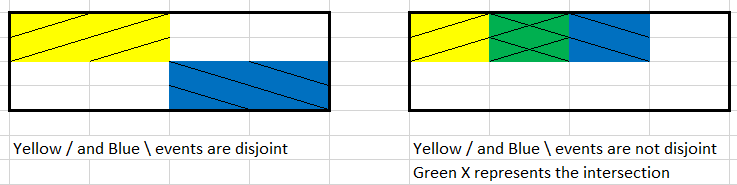
\includegraphics[width=2.46in,height=\textheight,keepaspectratio]{_graphics/venn-disjoint.png}

}

\caption{\label{fig-venn-disjoint}Illustration of countable additivity
for two events. The events in the picture on the left are disjoint, but
not on the right.}

\end{figure}%

The three axioms of a probability measure are simply minimal logical
consistency requirements that must be satisfied by any probability model
to ensure that probabilities fit together in a coherent way. There are
also many physical aspects of the random phenomenon or assumptions
(e.g.~``fairness'', independence, conditional relationships) that must
be considered when determining a reasonable probability measure for a
particular situation. Sometimes \(\textrm{P}(A)\) is defined explicitly
for an event \(A\) via a formula. But it is much more common for a
probability measure to be defined only implicitly through modeling
assumptions; probabilities of events then follow from the axioms and
related properties.

\subsection{Some probability measures for a four-sided
die}\label{some-probability-measures-for-a-four-sided-die}

\begin{tcolorbox}[enhanced jigsaw, opacityback=0, rightrule=.15mm, coltitle=black, colframe=quarto-callout-caution-color-frame, toprule=.15mm, colbacktitle=quarto-callout-caution-color!10!white, opacitybacktitle=0.6, left=2mm, toptitle=1mm, breakable, title={Caution}, bottomtitle=1mm, colback=white, leftrule=.75mm, titlerule=0mm, arc=.35mm, bottomrule=.15mm]

This section concerns a \emph{single} roll of a fair four-sided die.
Don't confuse this scenario with many other examples that involve
\emph{two} rolls. This section also discusses all possible \emph{events}
(beyond just all possible outcomes). We encourage you to review
Section~\ref{sec-sigmafield} before reading this section.

\end{tcolorbox}

Consider a \emph{single} roll of a four-sided die. The sample space
consists of four possible outcomes, \(\Omega = \{1, 2, 3, 4\}\). Events
concern what might happen on a single roll. For example, if \(A\) is the
event that we roll an odd number then \(A = \{1, 3\}\); ``roll an odd
number'' occurs if we roll a 1 so 1 is an \(A\), or ``roll an odd
number'' occurs if we roll a 3 so 3 is in \(A\).
Table~\ref{tbl-die-events} lists the collection of all events.

\begin{tcolorbox}[enhanced jigsaw, opacityback=0, rightrule=.15mm, coltitle=black, colframe=quarto-callout-caution-color-frame, toprule=.15mm, colbacktitle=quarto-callout-caution-color!10!white, opacitybacktitle=0.6, left=2mm, toptitle=1mm, breakable, title={Caution}, bottomtitle=1mm, colback=white, leftrule=.75mm, titlerule=0mm, arc=.35mm, bottomrule=.15mm]

We usually think of a table as a list of all possible \emph{outcomes},
with one row for each outcome. Table~\ref{tbl-die-events} and the tables
in this section (Table~\ref{tbl-die-events-fair},
Table~\ref{tbl-die-events-weighted},
Table~\ref{tbl-die-events-weighted2}) are different kinds of tables.
Each row of these tables is an \emph{event}, and the tables list the
collection of all events.

\end{tcolorbox}

\begin{tcolorbox}[enhanced jigsaw, opacityback=0, left=2mm, colframe=quarto-callout-note-color-frame, toprule=.15mm, breakable, colback=white, leftrule=.75mm, arc=.35mm, rightrule=.15mm, bottomrule=.15mm]

\begin{example}[]\protect\hypertarget{exm-die-measure-fair}{}\label{exm-die-measure-fair}

Let's first assume that the die is fair. Let \(\textrm{P}\) denote the
probability measure corresponding to a single roll of a fair four-sided
die.

\begin{enumerate}
\def\labelenumi{\arabic{enumi}.}
\tightlist
\item
  What is the probability that a single roll lands on 1? 2? 3? 4?
\item
  Compute the probability of each of the events in
  Table~\ref{tbl-die-events}.
\item
  Specify a general formula for \(\textrm{P}(A)\) for any event of
  interest \(A\) in this example.
\end{enumerate}

\end{example}

\end{tcolorbox}

\begin{tcolorbox}[enhanced jigsaw, opacityback=0, rightrule=.15mm, coltitle=black, colframe=quarto-callout-tip-color-frame, toprule=.15mm, colbacktitle=quarto-callout-tip-color!10!white, opacitybacktitle=0.6, left=2mm, toptitle=1mm, breakable, title={Solution (click to expand)}, bottomtitle=1mm, colback=white, leftrule=.75mm, titlerule=0mm, arc=.35mm, bottomrule=.15mm]

\begin{refsolution}
\leavevmode

\begin{enumerate}
\def\labelenumi{\arabic{enumi}.}
\tightlist
\item
  Assuming the die is fair implies that all four outcomes are equally
  likely, each with probability\footnotemark{} 1/4.
\item
  Given the probability of each outcome\footnotemark{}, we can find the
  probability of an event via countable additivity---sum the
  probabilities of the distinct outcomes that comprise the event. For
  example, if \(A=\{1, 3\}\) is the event that the die lands on an odd
  number, then \[
  \textrm{P}(A) = \textrm{P}(\{1, 3\}) = \textrm{P}(\{1\}\cup \{3\}) = \textrm{P}(\{1\}) + \textrm{P}(\{3\}) = 1/4+ 1/4 = 2/4.
  \] Table~\ref{tbl-die-events-fair} lists all the possible events, and
  their probabilities according to the probability measure
  \(\textrm{P}\).
\item
  Since there are four equally likely outcomes, the probability of any
  event is \[
  \textrm{P}(A) = \frac{\text{number of outcomes that satisfy $A$}}{4}, \qquad{\text{$\textrm{P}$ assumes a fair four-sided die}}
  \]
\end{enumerate}

\label{sol-die-measure-fair}

\end{refsolution}

\end{tcolorbox}

\footnotetext{That the probability of each outcome must be 1/4 when
there are four \emph{equally likely} outcomes follows from the axioms,
by writing \(\{1, 2, 3, 4\} = \{1\}\cup\{2\}\cup \{3\}\cup \{4\}\), a
union of disjoint sets, and applying countable additivity and
\(\textrm{P}(\Omega)=1\). But we don't need this level of technical
detail; our intuition tells us the probability of each four equally
likely outcomes is 1/4.}

\footnotetext{Probabilities are always defined for events (sets). When
we say loosely ``the probability of an outcome \(\omega\)'' we really
mean the probability of the event \(\{\omega\}\) consisting of the
single outcome \(\omega\). In this example
\(\textrm{P}(\{1\})=\textrm{P}(\{2\})=\textrm{P}(\{3\})=\textrm{P}(\{4\})=1/4\).}

\begin{longtable}[]{@{}
  >{\raggedright\arraybackslash}p{(\linewidth - 4\tabcolsep) * \real{0.3333}}
  >{\raggedright\arraybackslash}p{(\linewidth - 4\tabcolsep) * \real{0.3333}}
  >{\raggedright\arraybackslash}p{(\linewidth - 4\tabcolsep) * \real{0.3333}}@{}}
\caption{All possible events associated with a single roll of a
four-sided die, and their probabilities assuming the die is
fair.}\label{tbl-die-events-fair}\tabularnewline
\toprule\noalign{}
\begin{minipage}[b]{\linewidth}\raggedright
Event
\end{minipage} & \begin{minipage}[b]{\linewidth}\raggedright
Description
\end{minipage} & \begin{minipage}[b]{\linewidth}\raggedright
Probability of event assuming a fair die
\end{minipage} \\
\midrule\noalign{}
\endfirsthead
\toprule\noalign{}
\begin{minipage}[b]{\linewidth}\raggedright
Event
\end{minipage} & \begin{minipage}[b]{\linewidth}\raggedright
Description
\end{minipage} & \begin{minipage}[b]{\linewidth}\raggedright
Probability of event assuming a fair die
\end{minipage} \\
\midrule\noalign{}
\endhead
\bottomrule\noalign{}
\endlastfoot
\(\emptyset\) & Roll nothing (not possible) & 0 \\
\(\{1\}\) & Roll a 1 & 1/4 \\
\(\{2\}\) & Roll a 2 & 1/4 \\
\(\{3\}\) & Roll a 3 & 1/4 \\
\(\{4\}\) & Roll a 4 & 1/4 \\
\(\{1, 2\}\) & Roll a 1 or a 2 & 2/4 \\
\(\{1, 3\}\) & Roll a 1 or a 3 & 2/4 \\
\(\{1, 4\}\) & Roll a 1 or a 4 & 2/4 \\
\(\{2, 3\}\) & Roll a 2 or a 3 & 2/4 \\
\(\{2, 4\}\) & Roll a 2 or a 4 & 2/4 \\
\(\{3, 4\}\) & Roll a 3 or a 4 & 2/4 \\
\(\{1, 2, 3\}\) & Roll a 1, 2, or 3 (a.k.a. do not roll a 4) & 3/4 \\
\(\{1, 2, 4\}\) & Roll a 1, 2, or 4 (a.k.a. do not roll a 3) & 3/4 \\
\(\{1, 3, 4\}\) & Roll a 1, 3, or 4 (a.k.a. do not roll a 2) & 3/4 \\
\(\{2, 3, 4\}\) & Roll a 2, 3, or 4 (a.k.a. do not roll a 1) & 3/4 \\
\(\{1, 2, 3, 4\}\) & Roll something & 1 \\
\end{longtable}

When outcomes are equally likely, we find the probability of an event by
counting the number of outcomes that satisfy the event.

The probability measure \(\textrm{P}\) in
Example~\ref{exm-die-measure-fair} satisfies all the axioms and so it is
a valid probability measure. However, assuming that the outcomes are
equally likely is a much stricter condition than the basic logical
consistency requirements of the axioms. There are many other possible
probability measures, like in the following.

\begin{tcolorbox}[enhanced jigsaw, opacityback=0, left=2mm, colframe=quarto-callout-note-color-frame, toprule=.15mm, breakable, colback=white, leftrule=.75mm, arc=.35mm, rightrule=.15mm, bottomrule=.15mm]

\begin{example}[]\protect\hypertarget{exm-die-weighted}{}\label{exm-die-weighted}

Now consider a single roll of a four-sided die, but suppose the die is
weighted so that the outcomes are no longer equally likely. Suppose that
the probability of event \(\{2, 3\}\) is 0.5, of event \(\{3, 4\}\) is
0.7, and of event \(\{1, 2, 3\}\) is 0.6. Let \(\textrm{Q}\) denote the
probability measure corresponding to a single roll of this weighted
four-sided die.

\begin{enumerate}
\def\labelenumi{\arabic{enumi}.}
\tightlist
\item
  In what particular way is the die weighted? That is, what is the
  probability of each the four possible outcomes?
\item
  Complete a table, like Table~\ref{tbl-die-events-fair}, listing the
  probability of each event for this particular weighted die.
\end{enumerate}

\end{example}

\end{tcolorbox}

\begin{tcolorbox}[enhanced jigsaw, opacityback=0, rightrule=.15mm, coltitle=black, colframe=quarto-callout-tip-color-frame, toprule=.15mm, colbacktitle=quarto-callout-tip-color!10!white, opacitybacktitle=0.6, left=2mm, toptitle=1mm, breakable, title={Solution (click to expand)}, bottomtitle=1mm, colback=white, leftrule=.75mm, titlerule=0mm, arc=.35mm, bottomrule=.15mm]

\begin{refsolution}
\leavevmode

\begin{enumerate}
\def\labelenumi{\arabic{enumi}.}
\tightlist
\item
  Since the probability of event \(\{1, 2, 3\}\)---that is, not rolling
  a 4---is 0.6, the probability of rolling a 4 must be\footnotemark{}
  0.4. Since the probability of rolling a 3 or 4 is 0.7 and the
  probability of rolling a 4 is 0.4, the probability of rolling a 3 must
  be 0.3. Similarly, the probability of rolling a 2 must be 0.2, and the
  probability of rolling a 1 must be 0.1.
\item
  Given the probability of each outcome we can find the probability of
  an event by summing the probabilities of the distinct outcomes that
  comprise the event. For example, the probability that a single roll of
  this die lands on an odd number is \[
  \textrm{Q}(\{1, 3\}) = \textrm{Q}(\{1\}\cup \{3\}) = \textrm{Q}(\{1\}) + \textrm{Q}(\{3\}) = 0.1+ 0.3 = 0.4.
  \] We can similarly find the probabilities of all possible events for
  this particular weighted die, displayed in
  Table~\ref{tbl-die-events-weighted}.
\end{enumerate}

\label{sol-die-weighted}

\end{refsolution}

\end{tcolorbox}

\footnotetext{\(\Omega = \{1, 2, 3\} \cup \{4\}\), a union of disjoint
events, so
\(1 = \textrm{Q}(\Omega) = \textrm{Q}(\{1, 2, 3\}) + \textrm{Q}(\{4\})\).}

\begin{longtable}[]{@{}
  >{\raggedright\arraybackslash}p{(\linewidth - 4\tabcolsep) * \real{0.3333}}
  >{\raggedright\arraybackslash}p{(\linewidth - 4\tabcolsep) * \real{0.3333}}
  >{\raggedright\arraybackslash}p{(\linewidth - 4\tabcolsep) * \real{0.3333}}@{}}
\caption{All possible events associated with a single roll of a
four-sided die, and their probabilities assuming the die is weighted:
roll a 1 with probability 0.1, 2 with probability 0.2, 3 with
probability 0.3, 4 with probability
0.4.}\label{tbl-die-events-weighted}\tabularnewline
\toprule\noalign{}
\begin{minipage}[b]{\linewidth}\raggedright
Event
\end{minipage} & \begin{minipage}[b]{\linewidth}\raggedright
Description
\end{minipage} & \begin{minipage}[b]{\linewidth}\raggedright
Probability of event assuming a particular weighted die
\end{minipage} \\
\midrule\noalign{}
\endfirsthead
\toprule\noalign{}
\begin{minipage}[b]{\linewidth}\raggedright
Event
\end{minipage} & \begin{minipage}[b]{\linewidth}\raggedright
Description
\end{minipage} & \begin{minipage}[b]{\linewidth}\raggedright
Probability of event assuming a particular weighted die
\end{minipage} \\
\midrule\noalign{}
\endhead
\bottomrule\noalign{}
\endlastfoot
\(\emptyset\) & Roll nothing (not possible) & 0 \\
\(\{1\}\) & Roll a 1 & 0.1 \\
\(\{2\}\) & Roll a 2 & 0.2 \\
\(\{3\}\) & Roll a 3 & 0.3 \\
\(\{4\}\) & Roll a 4 & 0.4 \\
\(\{1, 2\}\) & Roll a 1 or a 2 & 0.3 \\
\(\{1, 3\}\) & Roll a 1 or a 3 & 0.4 \\
\(\{1, 4\}\) & Roll a 1 or a 4 & 0.5 \\
\(\{2, 3\}\) & Roll a 2 or a 3 & 0.5 \\
\(\{2, 4\}\) & Roll a 2 or a 4 & 0.6 \\
\(\{3, 4\}\) & Roll a 3 or a 4 & 0.7 \\
\(\{1, 2, 3\}\) & Roll a 1, 2, or 3 (a.k.a. do not roll a 4) & 0.6 \\
\(\{1, 2, 4\}\) & Roll a 1, 2, or 4 (a.k.a. do not roll a 3) & 0.7 \\
\(\{1, 3, 4\}\) & Roll a 1, 3, or 4 (a.k.a. do not roll a 2) & 0.8 \\
\(\{2, 3, 4\}\) & Roll a 2, 3, or 4 (a.k.a. do not roll a 1) & 0.9 \\
\(\{1, 2, 3, 4\}\) & Roll something & 1 \\
\end{longtable}

The symbol \(\textrm{P}\) is more than just shorthand for the word
``probability''. \(\textrm{P}\) denotes the underlying probability
measure, which represents all the assumptions about the random
phenomenon. Changing assumptions results in a change of the probability
measure and a different probability model. We often consider several
probability measures for the same sample space and collection of events;
these several measures represent different sets of assumptions or
available information and different probability models.

The probability measure \(\textrm{P}\) in
Example~\ref{exm-die-measure-fair} corresponds to the assumption of a
fair die (equally likely outcomes). With this measure
\(\textrm{P}(A) = 2/4=0.5\) for \(A = \{1, 3\}\). But under the
probability measure \(\textrm{Q}\) corresponding to the weighted die in
Example~\ref{exm-die-weighted}, \(\textrm{Q}(A) = 0.4\). The outcomes
and events are the same in both scenarios, because both scenarios
involve a four sided-die. What is different is the probability measure
that assigns probabilities to the events. One scenario assumes the die
is fair while the other assumes the die has a particular weighting,
resulting in two different probability measures.

Both probability measures \(\textrm{P}\) and \(\textrm{Q}\) can be
written as explicit set functions: for an event \(A\)

\begin{align*}
\textrm{P}(A) & = \frac{\text{number of outcomes that satisfy $A$}}{4}, & & {\text{a fair four-sided die}}
\\
\textrm{Q}(A) & = \frac{\text{sum of elements in $A$}}{10}, & & {\text{a specific weighted four-sided die}}
\end{align*}

We provide the above descriptions to illustrate that a probability
measure operates on sets. However, in many situations there does not
exist a simple closed form expression for the set function defining the
probability measure which maps events to probabilities.

\begin{tcolorbox}[enhanced jigsaw, opacityback=0, left=2mm, colframe=quarto-callout-note-color-frame, toprule=.15mm, breakable, colback=white, leftrule=.75mm, arc=.35mm, rightrule=.15mm, bottomrule=.15mm]

\begin{example}[]\protect\hypertarget{exm-dice-normalize}{}\label{exm-dice-normalize}

Consider again a single roll of a weighted four-sided die. Suppose that

\begin{itemize}
\tightlist
\item
  Rolling a 1 is twice as likely as rolling a 4
\item
  Rolling a 2 is three times as likely as rolling a 4
\item
  Rolling a 3 is 1.5 times as likely as rolling a 4
\end{itemize}

Let \(\tilde{\textrm{Q}}\) be the probability measure corresponding to
this die.

\begin{enumerate}
\def\labelenumi{\arabic{enumi}.}
\tightlist
\item
  In what particular way is the die weighted? That is, what is the
  probability of each the four possible outcomes?
\item
  Compute \(\tilde{\textrm{Q}}(A)\) for each event in
  Table~\ref{tbl-die-events-fair}.
\item
  Weighting a die in a particular way might be hard to conceptualize and
  even harder to achieve in practice. Construct a circular spinner to
  represent this weighted die.
\end{enumerate}

\end{example}

\end{tcolorbox}

\begin{tcolorbox}[enhanced jigsaw, opacityback=0, rightrule=.15mm, coltitle=black, colframe=quarto-callout-tip-color-frame, toprule=.15mm, colbacktitle=quarto-callout-tip-color!10!white, opacitybacktitle=0.6, left=2mm, toptitle=1mm, breakable, title={Solution (click to expand)}, bottomtitle=1mm, colback=white, leftrule=.75mm, titlerule=0mm, arc=.35mm, bottomrule=.15mm]

\begin{refsolution}
\leavevmode

\begin{enumerate}
\def\labelenumi{\arabic{enumi}.}
\item
  Let \(q = \tilde{\textrm{Q}}(\{4\})\) denote the probability of
  rolling a 4. Then \(\tilde{\textrm{Q}}(\{1\}) = 2q\),
  \(\tilde{\textrm{Q}}(\{2\}) = 3q\), and
  \(\tilde{\textrm{Q}}(\{3\}) = 1.5q\). Since these probabilities must
  sum to 1, we have \(2q + 3q + 1.5q + q = 1\) so \(q = 2/15\).
  Therefore, the probability of rolling a 1 is 4/15, a 2 is 6/15, a 3 is
  3/15, and a 4 is 2/15. (We could have also solved this without algebra
  similiar to how we solved Example~\ref{exm-worldseries-proportional}.)
\item
  Given the probability of each outcome we can find the probability of
  an event by summing the probabilities of the distinct outcomes that
  comprise the event. For example, the probability of rolling an odd
  number is \[
  \tilde{\textrm{Q}}(\{1, 3\}) = \tilde{\textrm{Q}}(\{1\}\cup \{3\}) = \tilde{\textrm{Q}}(\{1\}) + \tilde{\textrm{Q}}(\{3\}) = 4/15+ 3/15 = 7/15 \approx 0.467.
  \]

  We can similarly find the probabilities of all possible events for
  this particular weighted die, displayed in
  Table~\ref{tbl-die-events-weighted2}. Note this probability measure
  does not have a simple closed formula for \(\tilde{\textrm{Q}}(A)\).
\item
  Construct a spinner with four sectors of area 4/15, 6/15, 3/15, and
  2/15 representing, respectively, the values 1, 2, 3, and 4. See
  Figure~\ref{fig-die-three-spinners-3}.
\end{enumerate}

\label{sol-dice-normalize}

\end{refsolution}

\end{tcolorbox}

\begin{longtable}[]{@{}
  >{\raggedright\arraybackslash}p{(\linewidth - 4\tabcolsep) * \real{0.3333}}
  >{\raggedright\arraybackslash}p{(\linewidth - 4\tabcolsep) * \real{0.3333}}
  >{\raggedright\arraybackslash}p{(\linewidth - 4\tabcolsep) * \real{0.3333}}@{}}
\caption{All possible events associated with a single roll of a
four-sided die, and their probabilities assuming the die is weighted:
roll a 1 with probability 4/15, 2 with probability 6/15, 3 with
probability 3/15, 4 with probability
2/15.}\label{tbl-die-events-weighted2}\tabularnewline
\toprule\noalign{}
\begin{minipage}[b]{\linewidth}\raggedright
Event
\end{minipage} & \begin{minipage}[b]{\linewidth}\raggedright
Description
\end{minipage} & \begin{minipage}[b]{\linewidth}\raggedright
Probability of event assuming a particular weighted die
\end{minipage} \\
\midrule\noalign{}
\endfirsthead
\toprule\noalign{}
\begin{minipage}[b]{\linewidth}\raggedright
Event
\end{minipage} & \begin{minipage}[b]{\linewidth}\raggedright
Description
\end{minipage} & \begin{minipage}[b]{\linewidth}\raggedright
Probability of event assuming a particular weighted die
\end{minipage} \\
\midrule\noalign{}
\endhead
\bottomrule\noalign{}
\endlastfoot
\(\emptyset\) & Roll nothing (not possible) & 0 \\
\(\{1\}\) & Roll a 1 & 4/15 \\
\(\{2\}\) & Roll a 2 & 6/15 \\
\(\{3\}\) & Roll a 3 & 3/15 \\
\(\{4\}\) & Roll a 4 & 2/15 \\
\(\{1, 2\}\) & Roll a 1 or a 2 & 10/15 \\
\(\{1, 3\}\) & Roll a 1 or a 3 & 7/15 \\
\(\{1, 4\}\) & Roll a 1 or a 4 & 6/15 \\
\(\{2, 3\}\) & Roll a 2 or a 3 & 9/15 \\
\(\{2, 4\}\) & Roll a 2 or a 4 & 8/15 \\
\(\{3, 4\}\) & Roll a 3 or a 4 & 5/15 \\
\(\{1, 2, 3\}\) & Roll a 1, 2, or 3 (a.k.a. do not roll a 4) & 13/15 \\
\(\{1, 2, 4\}\) & Roll a 1, 2, or 4 (a.k.a. do not roll a 3) & 12/15 \\
\(\{1, 3, 4\}\) & Roll a 1, 3, or 4 (a.k.a. do not roll a 2) & 9/15 \\
\(\{2, 3, 4\}\) & Roll a 2, 3, or 4 (a.k.a. do not roll a 1) & 11/15 \\
\(\{1, 2, 3, 4\}\) & Roll something & 1 \\
\end{longtable}

The die rolling example is not the most exciting or practical scenario.
But the example does illustrate the idea of several probability
measures, each corresponding to a different set of assumptions about the
random phenomenon. If it's difficult to imagine how to physically weight
a die in these particular ways, consider the spinners (like from a kids
game) in Figure~\ref{fig-die-three-spinners}).

\begin{figure}

\begin{minipage}{0.33\linewidth}

\centering{

\pandocbounded{\includegraphics[keepaspectratio]{language-probability_files/figure-pdf/fig-die-three-spinners-1.png}}

}

\subcaption{\label{fig-die-three-spinners-1}A fair die}

\end{minipage}%
%
\begin{minipage}{0.33\linewidth}

\centering{

\pandocbounded{\includegraphics[keepaspectratio]{language-probability_files/figure-pdf/fig-die-three-spinners-2.png}}

}

\subcaption{\label{fig-die-three-spinners-2}The weighted die of
Example~\ref{exm-die-weighted}}

\end{minipage}%
%
\begin{minipage}{0.33\linewidth}

\centering{

\pandocbounded{\includegraphics[keepaspectratio]{language-probability_files/figure-pdf/fig-die-three-spinners-3.png}}

}

\subcaption{\label{fig-die-three-spinners-3}The weighted die of
Example~\ref{exm-dice-normalize}}

\end{minipage}%

\caption{\label{fig-die-three-spinners}Three possible spinners
corresponding to the roll of a four-sided die.}

\end{figure}%

\begin{tcolorbox}[enhanced jigsaw, opacityback=0, left=2mm, colframe=quarto-callout-note-color-frame, toprule=.15mm, breakable, colback=white, leftrule=.75mm, arc=.35mm, rightrule=.15mm, bottomrule=.15mm]

\begin{example}[]\protect\hypertarget{exm-dice-measures-interpret}{}\label{exm-dice-measures-interpret}

Using the set up of this section, the event \(A = \{1, 3\}\), and the
spinners from Figure~\ref{fig-die-three-spinners},

\begin{enumerate}
\def\labelenumi{\arabic{enumi}.}
\tightlist
\item
  Interpret each of \(\textrm{P}(A) = 0.5\), \(\textrm{Q}(A) = 0.4\),
  and \(\tilde{\textrm{Q}}(A) = 7/15\) as a long run relative frequency.
\item
  Interpret each of \(\textrm{P}(A) = 0.5\), \(\textrm{Q}(A) = 0.4\),
  and \(\tilde{\textrm{Q}}(A) = 7/15\) in terms of a relative degree of
  likelihood.
\end{enumerate}

\end{example}

\end{tcolorbox}

\begin{tcolorbox}[enhanced jigsaw, opacityback=0, rightrule=.15mm, coltitle=black, colframe=quarto-callout-tip-color-frame, toprule=.15mm, colbacktitle=quarto-callout-tip-color!10!white, opacitybacktitle=0.6, left=2mm, toptitle=1mm, breakable, title={Solution (click to expand)}, bottomtitle=1mm, colback=white, leftrule=.75mm, titlerule=0mm, arc=.35mm, bottomrule=.15mm]

\begin{refsolution}
\leavevmode

\begin{enumerate}
\def\labelenumi{\arabic{enumi}.}
\tightlist
\item
  Use the spinners from Figure~\ref{fig-die-three-spinners}.

  \begin{itemize}
  \tightlist
  \item
    \(\textrm{P}(A) = 0.5\): Spin the spinner on the left many times; it
    will land on an odd number on about 50\% of spins.
  \item
    \(\textrm{Q}(A) = 0.4\): Spin the spinner in the middle many times;
    it will land on an odd number on about 40\% of spins.
  \item
    \(\tilde{\textrm{Q}}(A) = 7/15\): Spin the spinner on the right many
    times; it will land on an odd number on about 46.67\% of spins.
  \end{itemize}
\item
  Use the spinners from Figure~\ref{fig-die-three-spinners}.

  \begin{itemize}
  \tightlist
  \item
    \(\textrm{P}(A) = 0.5\): The spinner on the left is equally likely
    to land on an odd number or an even number
  \item
    \(\textrm{Q}(A) = 0.4\): The spinner in the middle is 1.5 times more
    likely to land on an even number than on an odd number.
  \item
    \(\tilde{\textrm{Q}}(A) = 7/15\): The spinner on the right is
    \(8/7\approx 1.14\) times more likely to land on an even number than
    on an odd number.
  \end{itemize}
\end{enumerate}

\label{sol-dice-measures-interpret}

\end{refsolution}

\end{tcolorbox}

It is usually reasonable to assume that dice are fair, but most real
world situations are not as simple as rolling dice. Just because a
situation has 16 possible outcomes doesn't mean the outcomes have to be
equally likely. For example, there might be 12 contestants on your
favorite reality competition show, but that doesn't mean that all of the
12 contestants are equally likely to win the season.

\subsection{Some probability measures in the meeting
problem}\label{sec-meeting-probspace}

Recall the meeting problem. The general problem involves multiple
people, but we'll first consider the arrival time of just a single
person, who we'll call Han\footnote{Because he's solo.}.

\begin{tcolorbox}[enhanced jigsaw, opacityback=0, rightrule=.15mm, coltitle=black, colframe=quarto-callout-caution-color-frame, toprule=.15mm, colbacktitle=quarto-callout-caution-color!10!white, opacitybacktitle=0.6, left=2mm, toptitle=1mm, breakable, title={Caution}, bottomtitle=1mm, colback=white, leftrule=.75mm, titlerule=0mm, arc=.35mm, bottomrule=.15mm]

Some of the examples in this section involve just a single person
arriving, while other examples involve two people.

\end{tcolorbox}

Suppose that Han's arrival time will definitely be between noon and
1:00, so that the sample space---with time measured in minutes after
noon, including fractions of a minute---is \(\Omega = [0, 60]\).

\begin{tcolorbox}[enhanced jigsaw, opacityback=0, left=2mm, colframe=quarto-callout-note-color-frame, toprule=.15mm, breakable, colback=white, leftrule=.75mm, arc=.35mm, rightrule=.15mm, bottomrule=.15mm]

\begin{example}[]\protect\hypertarget{exm-meeting-probspace1d-uniform}{}\label{exm-meeting-probspace1d-uniform}

Suppose that Han arrives ``uniformly at random'' at a time in
\([0, 60]\). Use your intuition to provide your best guess for each of
the following probabilities.

\begin{enumerate}
\def\labelenumi{\arabic{enumi}.}
\tightlist
\item
  The probability that Han arrives before 12:30.
\item
  The probability that Han arrives before 12:15.
\item
  The probability that Han arrives after 12:45.
\item
  The probability that Han arrives between 12:15 and 12:45.
\item
  The probability that Han arrives before 12:05.
\item
  The probability that Han arrives between 12:15 and 12:20.
\item
  Let \(\textrm{P}\) denote the corresponding probability measure.
  Suggest a general formula for \(\textrm{P}([a, b])\), the probability
  that Han arrives between \(a\) and \(b\) minutes after noon for
  \(0\le a<b\le 60\) (e.g., \(a=15, b=20\) for ``between 12:15 and
  12:20'' or \(a = 0, b=5\) for ``before 12:05'').
\item
  Find the probability that Han's arrival time, truncated to the nearest
  minute, is 0 minutes after noon; that is, find the probability that
  Han arrives between 12:00 and 12:01.
\item
  Continue to find the probability that Han's arrival time
  truncated\footnotemark{} to the nearest minute is
  \(1, 2, 3, \ldots, 59\), and sketch a plot with arrival time
  (truncated minutes after noon) on the horizontal axis and probability
  on the vertical axis. Is the plot what you would expect for arriving
  ``uniformly at random''?
\end{enumerate}

\end{example}

\end{tcolorbox}

\footnotetext{It doesn't really matter if we round or truncate to the
nearest minute, but we're truncating so we don't treat 0 differently
than the other values (technically only times in the first 30 seconds,
not minute, round to 0).}

\begin{tcolorbox}[enhanced jigsaw, opacityback=0, rightrule=.15mm, coltitle=black, colframe=quarto-callout-tip-color-frame, toprule=.15mm, colbacktitle=quarto-callout-tip-color!10!white, opacitybacktitle=0.6, left=2mm, toptitle=1mm, breakable, title={Solution (click to expand)}, bottomtitle=1mm, colback=white, leftrule=.75mm, titlerule=0mm, arc=.35mm, bottomrule=.15mm]

\begin{refsolution}
``Uniformly at random'' means that in some sense Han is ``equally
likely'' to arrive at any time between noon and 1:00.

\begin{enumerate}
\def\labelenumi{\arabic{enumi}.}
\tightlist
\item
  0.5. It seems that Han should be as likely to arrive before 12:30 as
  after.
\item
  0.25. The time interval before 12:15 is 0.25 of the total noon to 1:00
  time interval, so if he is ``equally likely'' to arrive at any time,
  the probability that he arrives in a 15 minute interval is
  \(15/60 = 0.25\).
\item
  0.25. Similar to the previous part.
\item
  0.5. This 30 minute interval makes up half of the total noon to 1:00
  time interval.
\item
  \(1/12 = 0.083\). The time interval before 12:05 is \(5/60=1/12\) of
  the total noon to 1:00 time interval, so if he is ``equally likely''
  to arrive at any time, the probability that he arrives in a 5 minute
  interval is \(5/60 = 1/12=0.083\).
\item
  1/12, similar to the previous part.
\item
  It seems reasonable that if Han arrives uniformly at random within the
  60 minute time interval, the probability that he arrives within any
  time interval \([a, b]\) (in \([0, 60]\)) is
  \(\textrm{P}([a, b]) = (b-a)/60\), the length of the time interval of
  interest divided by the length of the total time interval.
\item
  The probability that Han arrives in the one minute interval between
  12:00 and 12:01 is \(1/60\approx 0.0167\).
\item
  The probability that Han arrives in any one minute interval is
  \(1/60\approx 0.0167\). See
  Figure~\ref{fig-arrival-time-probmeasure-uniform}.
\end{enumerate}

\label{sol-meeting-probspace1d-uniform}

\end{refsolution}

\end{tcolorbox}

\begin{figure}

\centering{

\pandocbounded{\includegraphics[keepaspectratio]{language-probability_files/figure-pdf/fig-arrival-time-probmeasure-uniform-1.png}}

}

\caption{\label{fig-arrival-time-probmeasure-uniform}Probability of Han
arriving at each minute between noon (0) and 1:00 (60), truncated to the
nearest minute, for the uniform probability measure in
Example~\ref{exm-meeting-probspace1d-uniform}).}

\end{figure}%

Example~\ref{exm-die-measure-fair} illustrated that for a finite sample
space with equally likely outcomes, computing the probability of an
event reduces to counting the number of outcomes that satisfy the event
and dividing by the total number of possible outcomes. The continuous
analog of equally likely outcomes is a \emph{uniform probability
measure}. When the sample space is uncountable, size is measured
continuously (length, area, volume) rather that discretely (counting).

\[
\textrm{P}(A) = \frac{\text{size of } A}{\text{size of } \Omega} \qquad \text{if $\textrm{P}$ is a uniform probability measure}
\]

The uniform probability measure in
Example~\ref{exm-meeting-probspace1d-uniform} is just one probability
measure for Han's arrival, reflecting an assumption that Han is
``equally likely'' to arrive at any time between noon and 1:00. Now
we'll model Han's arrival time with a non-uniform probability measure
which reflects that he is more likely to arrive near certain times than
others.

\begin{tcolorbox}[enhanced jigsaw, opacityback=0, left=2mm, colframe=quarto-callout-note-color-frame, toprule=.15mm, breakable, colback=white, leftrule=.75mm, arc=.35mm, rightrule=.15mm, bottomrule=.15mm]

\begin{example}[]\protect\hypertarget{exm-meeting-nonuniform-probspace1}{}\label{exm-meeting-nonuniform-probspace1}

Assume that the probability that Han arrives between \(a\) and \(b\)
minutes after noon is \((b/60)^2 - (a/60)^2\) (for \(0\le a<b\le 60\)) .
Let \(\textrm{Q}\) denote the corresponding probability measure; notice
that \(\textrm{Q}([0, 60]) = (60/60)^2 - (0/60)^2 = 1\). (We will see
where such a probability measure might come from later. For now, we'll
just use it to compute probabilities and observe that it is a
non-uniform measure.) Compute the following probabilities and compare
your answers to the corresponding parts from
Example~\ref{exm-meeting-probspace1d-uniform}.

\begin{enumerate}
\def\labelenumi{\arabic{enumi}.}
\tightlist
\item
  The probability that Han arrives before 12:30.
\item
  The probability that Han arrives before 12:15.
\item
  The probability that Han arrives after 12:45.
\item
  The probability that Han arrives between 12:15 and 12:45.
\item
  Find the probability Han's arrival time, truncated to the nearest
  minute, is 0 minutes after noon; that is, find the probability that
  Han arrives between 12:00 and 12:01.
\item
  Continue to find the probability that Han's arrival time truncated to
  the nearest minute is \(1, 2, 3, \ldots, 59\), and sketch a plot with
  arrival time (truncated minutes after noon) on the horizontal axis and
  probability on the vertical axis. What assumptions about Han's arrival
  time does this probability measure reflect?
\end{enumerate}

\end{example}

\end{tcolorbox}

\begin{tcolorbox}[enhanced jigsaw, opacityback=0, rightrule=.15mm, coltitle=black, colframe=quarto-callout-tip-color-frame, toprule=.15mm, colbacktitle=quarto-callout-tip-color!10!white, opacitybacktitle=0.6, left=2mm, toptitle=1mm, breakable, title={Solution (click to expand)}, bottomtitle=1mm, colback=white, leftrule=.75mm, titlerule=0mm, arc=.35mm, bottomrule=.15mm]

\begin{refsolution}
\leavevmode

\begin{enumerate}
\def\labelenumi{\arabic{enumi}.}
\tightlist
\item
  The probability Han arrives before 12:30 is
  \(\textrm{Q}([0, 30]) = (30/60)^2 - (0/60)^2 =0.5^2 =0.25\). Han is 3
  times more likely to arrive after 12:30 than before 12:30. (Han is now
  less likely to arrive before 12:30 than in the uniform case.)
\item
  The probability Han arrives before 12:15 is
  \(\textrm{Q}([0, 15)) = (15/60)^2 - (0/60)^2 =0.25^2 = 0.0625\);
  \(\textrm{Q}([0, 15)) = 0.0625\). Han is 15 times more likely to
  arrive after 12:15 than before 12:15. (Han is now less likely to
  arrive within 15 minutes of noon than in the uniform case.)
\item
  The probability Han arrives before 12:45 is
  \(\textrm{Q}([0, 45)) = (45/60)^2 - (0/60)^2 =0.75^2 = 0.5625\).
  Therefore, the probability that Hans arrives after 12:45 is
  \(\textrm{Q}([45, 60]) = 1 - 0.5625 = 0.4375\). Han is 7 times more
  likely to arrive within 15 minutes of 1:00 than within 15 minutes of
  noon. (Han is now more likely to arrive with 15 minutes of 1:00 than
  in the uniform case.)
\item
  The probability that Han arrives between 12:15 and 12:45 is
  \(\textrm{Q}((15, 45)) = (45/60)^2-(15/60)^2 = 0.5\). (This
  probability happens to be the same as in the uniform case.)
\item
  \(\textrm{Q}([0, 1]) = (1/60)^2 - (0/60)^2 = 1/3600 = 0.000278\) is
  the probability that Han arrives within 1 minute of noon. (This
  probability is less than what it was in the uniform case.)
\item
  Continue as in the previous part. For example,
  \(\textrm{Q}([1, 2]) = (2/60)^2 - (1/60)^2 = 3/3600 = 0.000833\) is
  the probability that Han arrives between 12:01 and 12:02;
  \(\textrm{Q}([2, 3]) = (3/60)^2 - (2/60)^2 = 5/3600 = 0.000833\) is
  the probability that Han arrives between 12:01 and 12:02;
  \(\textrm{Q}([59, 60]) = (60/60)^2 - (59/60)^2 = 119/3600 = 0.033\) is
  the probability that Han arrives within 1 minute of 1:00. In general,
  \(\textrm{Q}([a, a+1]) = ((a+1)/60)^2 - (a/60)^2 = (2a+1)/3600\) for
  \(a = 0, 1, \ldots, 59\). See
  Figure~\ref{fig-arrival-time-probmeasure-uniform}. This probability
  measure assumes that Han is more likely to arrive closer to 1:00 than
  to noon.
\end{enumerate}

\label{sol-meeting-nonuniform-probspace1}

\end{refsolution}

\end{tcolorbox}

\begin{figure}

\centering{

\pandocbounded{\includegraphics[keepaspectratio]{language-probability_files/figure-pdf/fig-arrival-time-probmeasure-1.png}}

}

\caption{\label{fig-arrival-time-probmeasure}Probability of Han arriving
at each minute between noon (0) and 1:00 (60), truncated to the nearest
minute, for a uniform probability measure (blue) and the probability
measure in Example~\ref{exm-meeting-nonuniform-probspace1} (orange).}

\end{figure}%

The probability measure in
Example~\ref{exm-meeting-nonuniform-probspace1} is a non-uniform
measure. Han is much more likely to arrive between 12:45 and 1:00 than
between 12:00 and 12:15, even though both these intervals have the same
length.

\begin{tcolorbox}[enhanced jigsaw, opacityback=0, rightrule=.15mm, coltitle=black, colframe=quarto-callout-warning-color-frame, toprule=.15mm, colbacktitle=quarto-callout-warning-color!10!white, opacitybacktitle=0.6, left=2mm, toptitle=1mm, breakable, title={Warning}, bottomtitle=1mm, colback=white, leftrule=.75mm, titlerule=0mm, arc=.35mm, bottomrule=.15mm]

Be careful when reading Figure~\ref{fig-arrival-time-probmeasure}! For
example, the probability that the arrival time \emph{truncated to the
nearest minute} is 0 is 1/60 for the uniform measure in
Example~\ref{exm-meeting-probspace1d-uniform} and 1/3600 for the
non-uniform measure in Example~\ref{exm-meeting-nonuniform-probspace1};
these probabilities represent the probability that Han arrives
\emph{within one minute of noon} rather than the probability that Han
arrives exactly at noon. Likewise, the probability that the arrival time
\emph{truncated to the nearest minute} is 59 is 0.0167 = 60/3600 for the
uniform measure in Example~\ref{exm-meeting-probspace1d-uniform} and
0.033 = 119/3600 for the non-uniform measure in
Example~\ref{exm-meeting-nonuniform-probspace1}; these probabilities
represent the probability that Han arrives \emph{within one minute of
1:00} rather than the probability that Han arrives exactly at 1:00. All
of the dots in Figure~\ref{fig-arrival-time-probmeasure} correspond to
\emph{one-minute intervals}, not exact time points.

\end{tcolorbox}

\begin{tcolorbox}[enhanced jigsaw, opacityback=0, left=2mm, colframe=quarto-callout-note-color-frame, toprule=.15mm, breakable, colback=white, leftrule=.75mm, arc=.35mm, rightrule=.15mm, bottomrule=.15mm]

\begin{example}[]\protect\hypertarget{exm-meeting-probspace1d-limit}{}\label{exm-meeting-probspace1d-limit}

Continuing with the uniform probability measure of
Example~\ref{exm-meeting-probspace1d-uniform}.

\begin{enumerate}
\def\labelenumi{\arabic{enumi}.}
\tightlist
\item
  Find the probability that Han arrives between 12:00 and 12:01, within
  1 minute after noon.
\item
  Find the probability that Han arrives between 12:00:00 and 12:00:01,
  within 1 second after noon.
\item
  Find the probability that Han arrives between 12:00:00.000 and
  12:01:00.001, within 1 millisecond after noon.
\item
  Find the probability that Han arrives at the exact time
  12:00:00.00000\ldots{} (with infinite precision).
\end{enumerate}

\end{example}

\end{tcolorbox}

\begin{tcolorbox}[enhanced jigsaw, opacityback=0, rightrule=.15mm, coltitle=black, colframe=quarto-callout-tip-color-frame, toprule=.15mm, colbacktitle=quarto-callout-tip-color!10!white, opacitybacktitle=0.6, left=2mm, toptitle=1mm, breakable, title={Solution (click to expand)}, bottomtitle=1mm, colback=white, leftrule=.75mm, titlerule=0mm, arc=.35mm, bottomrule=.15mm]

\begin{refsolution}
For the uniform probability measure, the probability of arriving in any
interval is the length of the time interval divided by the length of the
total interval. With time measured in minutes, a one minute interval has
length 1, a one second interval has length \(1/60\), and a one
millisecond interval has length \(1/60000\).

\begin{enumerate}
\def\labelenumi{\arabic{enumi}.}
\tightlist
\item
  \(1/60 = 0.0167\) is Han's probability of arriving in this 1 minute
  interval.
\item
  \((1/60)/60 = 0.000278\) is Han's probability of arriving in this 1
  second interval.
\item
  \((1/60000)/60 = 0.000000278\) is Han's probability of arriving in
  this 1 millisecond interval
\item
  The exact time 12:00:00.0000 represents a single point the sample
  space, an interval of length 0. The probability that Han arrives at
  the exact time 12:00:00000 (with infinite precision) is 0;
  \(\textrm{P}(\{0\}) = 0\).
\end{enumerate}

\label{sol-meeting-probspace1d-limit}

\end{refsolution}

\end{tcolorbox}

The last part in Example~\ref{exm-meeting-probspace1d-limit} might seem
counterintuitive at first. There was nothing special about 12:00; pick
any precise time in the continuous interval from noon to 1:00, and the
probability that Han arrives at that exact time, with infinite
precision, is 0. This idea can be understood as a limit. The probability
that Han arrives within one minute of the specified time is small,
within one second of the specified time is even smaller, within one
millisecond of the specified time is even smaller still; with infinite
precision these time increments can get smaller and smaller
indefinitely. Of course, infinite precision is not practical, but
assuming the possible arrival times are represented by a continuous
interval provides a reasonable mathematical model. Even though any
particular time has probability 0 of being the precise arrival time,
\emph{intervals} of time still have positive probability of containing
the arrival time. When we ask a question like ``what is the probability
that Han arrives \emph{at noon}'', ``at noon'' really means ``within 1
minute of noon'' or ``within 1 second of noon'' or within whatever
degree of precision is good enough for our practical purposes, and such
intervals have non-zero probability.

\begin{tcolorbox}[enhanced jigsaw, opacityback=0, left=2mm, colframe=quarto-callout-note-color-frame, toprule=.15mm, breakable, colback=white, leftrule=.75mm, arc=.35mm, rightrule=.15mm, bottomrule=.15mm]

\begin{example}[]\protect\hypertarget{exm-meeting-probspace1d-limit-nonuniform}{}\label{exm-meeting-probspace1d-limit-nonuniform}

Continuing with the non-uniform probability measure of
Example~\ref{exm-meeting-nonuniform-probspace1}.

\begin{enumerate}
\def\labelenumi{\arabic{enumi}.}
\tightlist
\item
  Find the probability that Han arrives between 12:00 and 12:01, within
  1 minute after noon.
\item
  Find the probability that Han arrives between 12:00:00 and 12:00:01,
  within 1 second after noon.
\item
  Find the probability that Han arrives between 12:00:00.000 and
  12:01:00.001, within 1 millisecond after noon.
\item
  Find the probability that Han arrives at the exact time
  12:00:00.00000\ldots{} (with infinite precision).
\item
  Find the probability that Han arrives between 12:59 and 1:00, within 1
  minute before 1:00.
\item
  Find the probability that Han arrives between 12:59:59 and 1:00:00,
  within 1 second before 1:00.
\item
  Find the probability that Han arrives between 12:59:59.999 and
  1:00:00.000, within 1 millisecond before 1:00.
\item
  Find the probability that Han arrives at the exact time
  1:00:00.00000\ldots{} (with infinite precision).
\item
  Which is more likely: that Han arrives ``at noon'' or ``at 1:00''?
  Explain.
\end{enumerate}

\end{example}

\end{tcolorbox}

\begin{tcolorbox}[enhanced jigsaw, opacityback=0, rightrule=.15mm, coltitle=black, colframe=quarto-callout-tip-color-frame, toprule=.15mm, colbacktitle=quarto-callout-tip-color!10!white, opacitybacktitle=0.6, left=2mm, toptitle=1mm, breakable, title={Solution (click to expand)}, bottomtitle=1mm, colback=white, leftrule=.75mm, titlerule=0mm, arc=.35mm, bottomrule=.15mm]

\begin{refsolution}
With time measured in minutes, one minute is 1, one second is \(1/60\),
and one millisecond is \(1/60000\).

\begin{enumerate}
\def\labelenumi{\arabic{enumi}.}
\tightlist
\item
  \((1/60)^2 - 0 = 0.000278\) is Han's probability of arriving within 1
  minute of noon.
\item
  \(((1/60)/60)^2 - 0 = 0.000000077\) is Han's probability of arriving
  within 1 second of noon.
\item
  \(((1/60000)/60)^2 - 0= 0.000000000000077\) is Han's probability of
  arriving within 1 millisecond of noon.
\item
  The exact time 12:00:00.0000 represents a single point the sample
  space, an interval of length 0. The probability that Han arrives at
  the exact time 12:00:00000 (with infinite precision) is 0;
  \(\textrm{Q}(\{0\}) = 0\).
\item
  \(1-((60 - 1)/60)^2 = 0.033\) is Han's probability of arriving within
  1 minute of 1:00.
\item
  \(1-((60 - 1/60)/60)^2  = 0.00055\) is Han's probability of arriving
  within 1 second of 1:00.
\item
  \(1-((60 - 1/60000)/60)^2  = 0.00000055\) is Han's probability of
  arriving within 1 millisecond of 1:00.
\item
  The exact time 1:00:00.0000 represents a single point the sample
  space, an interval of length 0. The probability that Han arrives at
  the exact time 1:00:00000 (with infinite precision) is 0;
  \(\textrm{Q}(\{60\}) = 0\).
\item
  The probabilities of arriving precisely at noon or 1:00 are both 0.
  However, the probability of arriving ``close to'' 1:00 is greater than
  the probability of arriving ``close to'' noon, regardless of how
  ``close to'' is defined (within 1 minute, within 1 second, etc). In
  practice, ``at'' is probably best interpreted as ``close to'', and in
  this sense Han is more likely to arrive ``at 1:00'' than ``at noon''.
\end{enumerate}

\label{sol-meeting-probspace1d-limit-nonuniform}

\end{refsolution}

\end{tcolorbox}

Continuous sample spaces introduce some complications that we didn't
encounter when dealing with discrete sample spaces. For a continuous
sample space, the probability of any particular outcome\footnote{This is
  one reason why probabilities are defined directly for events and not
  outcomes.} is 0. However,
Example~\ref{exm-meeting-probspace1d-limit-nonuniform} illustrates that
in some sense certain outcomes can be more likely than others; Han is
more likely to arrive \emph{close to} 1:00 than \emph{close to} noon.
For continuous sample spaces it makes more sense to consider ``close
to'' probabilities rather than ``equals to'' probabilities. We will
investigate related ideas in much more detail as we go.

Now we'll return to the two-person (Regina, Cady) meeting problem from
Example~\ref{exm-meeting-outcome}, with sample space depicted in
Figure~\ref{fig-meeting-independent-uniform}. We will use pictures to
represent a few probability measures corresponding to different
assumptions about the arrival times. In the pictures below, lighter
colors represent regions of outcomes that are more likely; darker
colors, less likely.

Figure~\ref{fig-meeting-probmeasure1} corresponds to a uniform
probability measure under which all outcomes are ``equally likely''.
This probability measure would be appropriate if we assume that Regina
and Cady each arrive at a time uniformly at random between noon and 1,
independently of each other.

\begin{figure}

\centering{

\pandocbounded{\includegraphics[keepaspectratio]{language-probability_files/figure-pdf/fig-meeting-probmeasure1-1.png}}

}

\caption{\label{fig-meeting-probmeasure1}A uniform probability measure
in the (Regina, Cady) meeting problem.}

\end{figure}%

\begin{tcolorbox}[enhanced jigsaw, opacityback=0, left=2mm, colframe=quarto-callout-note-color-frame, toprule=.15mm, breakable, colback=white, leftrule=.75mm, arc=.35mm, rightrule=.15mm, bottomrule=.15mm]

\begin{example}[]\protect\hypertarget{exm-meeting-probspace2}{}\label{exm-meeting-probspace2}

Assume the uniform probability measure \(\textrm{P}\) represented by
Figure~\ref{fig-meeting-probmeasure1}. Hint: when finding probabilities
below, recall Example~\ref{exm-meeting-event} and
Figure~\ref{fig-meeting-probspace2-plot}.

\begin{enumerate}
\def\labelenumi{\arabic{enumi}.}
\tightlist
\item
  Find the probability that Regina arrives after Cady.
\item
  Find the probability that either Regina or Cady arrives before 12:30.
\item
  Find the probability that Cady arrives first and Regina arrives at
  most 15 minutes after Cady.
\item
  Find the probability that Regina arrives before 12:24.
\end{enumerate}

\end{example}

\end{tcolorbox}

\begin{tcolorbox}[enhanced jigsaw, opacityback=0, rightrule=.15mm, coltitle=black, colframe=quarto-callout-tip-color-frame, toprule=.15mm, colbacktitle=quarto-callout-tip-color!10!white, opacitybacktitle=0.6, left=2mm, toptitle=1mm, breakable, title={Solution (click to expand)}, bottomtitle=1mm, colback=white, leftrule=.75mm, titlerule=0mm, arc=.35mm, bottomrule=.15mm]

\begin{refsolution}
For a uniform probability measure, the probability of an event is the
size of the event divided by the size of the sample space. Since the
sample space is \([0, 60]\times[0, 60]\), a continuous two-dimensional
region, size is measured by area. The sample space has area 3600.

See Figure~\ref{fig-meeting-probspace2-plot} for pictures of the events
of interest.

\begin{enumerate}
\def\labelenumi{\arabic{enumi}.}
\tightlist
\item
  The triangular region corresponding to the event that Regina arrives
  after Cady has area 3600/2 = 1800. So the probability that Regina
  arrives after Cady is \(1800/3600=0.5\).
\item
  The L-shaped region corresponding to the event that Regina or Cady
  arrives before 12:30 has area \((0.75)(3600)\), so the probability is
  0.75.
\item
  The trapezoidal region corresponding to the event that that Regina
  arrives at most 15 minutes after Cady (and Cady arrives first) has
  area \((7/32)(3600) = (0.21875)(3600)\). (It's easiest to find the
  area of the two unshaded triangles and subtract from the total area of
  3600: \(3600 - 0.5(3600) - (3600)(1-0.25)^2/2=7/32(3600)\).) So the
  probability that Regina arrives at most 15 minutes after Cady (and
  Cady arrives first) is 0.21875.
\item
  The rectangular region corresponding to the event that that Regina
  arrives before 12:24 has area (0.4)(3600), so the probability is 0.4.
\end{enumerate}

\label{sol-meeting-probspace2}

\end{refsolution}

\end{tcolorbox}

\begin{figure}

\centering{

\pandocbounded{\includegraphics[keepaspectratio]{language-probability_files/figure-pdf/fig-meeting-probspace2-plot-1.png}}

}

\caption{\label{fig-meeting-probspace2-plot}Illustration of the events
in Exercise Example~\ref{exm-meeting-probspace2}. The square represents
the sample space. With a uniform probability measure, the areas of the
shaded regions relative to the whole represent their probabilities.}

\end{figure}%

\begin{tcolorbox}[enhanced jigsaw, opacityback=0, left=2mm, colframe=quarto-callout-note-color-frame, toprule=.15mm, breakable, colback=white, leftrule=.75mm, arc=.35mm, rightrule=.15mm, bottomrule=.15mm]

\begin{example}[]\protect\hypertarget{exm-meeting-probspace2-limit}{}\label{exm-meeting-probspace2-limit}

Continuing Example~\ref{exm-meeting-probspace2}

\begin{enumerate}
\def\labelenumi{\arabic{enumi}.}
\tightlist
\item
  Find the probability that Cady arrives first and Regina arrives at
  most 1 minute after Cady.
\item
  Find the probability that Cady arrives first and Regina arrives at
  most 1 second after Cady.
\item
  Find the probability that Cady arrives first and Regina arrives at
  most 1 millisecond after Cady.
\item
  Find the probability that Regina and Cady arrive at exactly the same
  time, with infinite precision.
\end{enumerate}

\end{example}

\end{tcolorbox}

\begin{tcolorbox}[enhanced jigsaw, opacityback=0, rightrule=.15mm, coltitle=black, colframe=quarto-callout-tip-color-frame, toprule=.15mm, colbacktitle=quarto-callout-tip-color!10!white, opacitybacktitle=0.6, left=2mm, toptitle=1mm, breakable, title={Solution (click to expand)}, bottomtitle=1mm, colback=white, leftrule=.75mm, titlerule=0mm, arc=.35mm, bottomrule=.15mm]

\begin{refsolution}
\leavevmode

\begin{enumerate}
\def\labelenumi{\arabic{enumi}.}
\tightlist
\item
  Similar to part 3 of Example~\ref{exm-meeting-probspace2}, the
  probability that Regina arrives at most 1 minute after Cady (and Cady
  arrives first) is \(1 - 0.5 - (1-1/60)^2/2=0.0165\).
\item
  The probability that Regina arrives at most 1 second after Cady (and
  Cady arrives first) is \(1 - 0.5 - (1-1/3600)^2/2=0.000278\).
\item
  The probability that Regina arrives at most 1 millisecond after Cady
  (and Cady arrives first) is
  \(1 - 0.5 - (1-1/3600000)^2/2=0.000000278\).
\item
  The event that Regina and Cady arrive at exactly the same time, with
  infinite precision, corresponds to the ``Regina = Cady'' line segment.
  The area of this line segment is 0, so the probability that Regina and
  Cady arrive at exactly the same time, with infinite precision, is 0.
\end{enumerate}

\label{sol-meeting-probspace2-limit}

\end{refsolution}

\end{tcolorbox}

Example~\ref{exm-meeting-probspace2-limit} and
Example~\ref{exm-meeting-probspace1d-limit} illustrate similar ideas.
Regardless of the precise time in the continuous interval \([0, 60]\) at
which Regina arrives, the probability that Cady arrives at that exact
time, with infinite precision, is 0. In practice, if we're interested in
``the probability that Regina at Cady arrive \emph{at the same time}'',
we really mean ``close enough to the same time'', where ``close enough''
could be within one minute or one second or whatever degree of precision
is good enough for practical purposes.

Most random phenomenon do not involve equally likely outcomes or uniform
probability measures. Even when the underlying outcomes are equally
likely, the values of related random variables are usually not.
Therefore, most interesting probability problems involve ``non-uniform''
probability measures.

Figure~\ref{fig-meeting-independent-normal} corresponds to one
non-uniform probability measure for the two-person meeting problem;
certain outcomes are more likely than others. (Lighter colors represent
regions of outcomes that are more likely; darker colors, less likely.)
Such a probability measure would be appropriate if we assume that Regina
and Cady each are more likely to arrive around 12:30 than noon or 1:00,
independently of each other. Switching from the uniform probability
measure represented by Figure~\ref{fig-meeting-probmeasure1} to the
non-uniform one represented by
Figure~\ref{fig-meeting-independent-normal} would change the probability
of the events in Example~\ref{exm-meeting-probspace2} and
Example~\ref{exm-meeting-probspace2-limit}. (We'll see how to compute
probabilities for non-uniform measures later.)

\begin{figure}

\centering{

\pandocbounded{\includegraphics[keepaspectratio]{language-probability_files/figure-pdf/fig-meeting-independent-normal-1.png}}

}

\caption{\label{fig-meeting-independent-normal}A non-uniform probability
measure in the two person meeting problem. Lighter colors represent
regions of outcomes that are more likely; darker colors, less likely.}

\end{figure}%

Figure~\ref{fig-meeting-dependent-normal} corresponds to another
``non-uniform'' probability measure. Such a probability measure would be
appropriate if we assume that Regina and Cady each are more likely to
arrive around 12:30 than noon or 1:00, but they coordinate their
arrivals so they are more likely to arrive around the same time.

\begin{figure}

\centering{

\pandocbounded{\includegraphics[keepaspectratio]{language-probability_files/figure-pdf/fig-meeting-dependent-normal-1.png}}

}

\caption{\label{fig-meeting-dependent-normal}Another non-uniform
probability measure in the two person meeting problem. Lighter colors
represent regions of outcomes that are more likely; darker colors, less
likely. Notice how the probability is concentrated along the \(R=Y\)
line}

\end{figure}%

There are many other probability measures for the meeting problem,
representing different sets of assumptions. Each probability measure
assigns a probability to events like ``Cady arrives first'', ``both
arrive before 12:20'', and ``the first person to arrive has to wait less
than 15 minutes for the second to arrive'', and these probabilities can
differ between models.

\subsection{Some properties of probability
measures}\label{some-properties-of-probability-measures}

Many other properties follow from the axioms, some of which we state
below. Don't let notation or names like the ``complement rule'' confuse
you. We have already successfully used all of the properties below
intuitively when working with two-way tables. All that is new in this
section is mathematical formalism. Yes, getting comfortable with proper
notation is part of learning the language of probability. But don't let
formality get in the way of your intuition. Continue to use the ideas
from Chapter~\ref{sec-prob-literacy}, including tools like two-way
tables.

The main ``meat'' of the axioms is countable additivity. Thus, the key
to many proofs of probability properties is to express relevant events
in terms of unions of disjoint events. (Proof are included in the
footnotes.)

\begin{lemma}[Complement
rule]\protect\hypertarget{lem-complement-rule}{}\label{lem-complement-rule}

\index{complement rule} For any event\footnote{\emph{Proof.} Since
  \(\Omega = A \cup A^c\) and \(A\) and \(A^c\) are disjoint the axioms
  imply that
  \(1=\textrm{P}(\Omega) = \textrm{P}(A \cup A^c) = \textrm{P}(A) + \textrm{P}(A^c)\).}
\(A\), \(\textrm{P}(A^c) = 1 - \textrm{P}(A)\).\index{complement rule}

\end{lemma}

The complement rule follows from the fact that an event either happens
or it doesn't. We'll see that it is sometimes more convenient to compute
directly the probability that an event does not happen and then use the
complement rule. Subtracting a computed probability from 1 seems like a
small computational step, but it's an important one. If you're taking a
test, a 0.9 probability of getting a question correct is much different
than a 0.1 probability. Unfortunately, the complement rule step is often
overlooked when doing probability calculations. It's a good idea to ask
yourself if the probability you are computing should be greater than or
less than 0.5. If your computed value seems to be on the wrong side of
0.5, check your calculations to see if you have forgotten (or
misapplied) the complement rule.

\begin{lemma}[Subset
rule]\protect\hypertarget{lem-subset-rule}{}\label{lem-subset-rule}

\index{subset rule} If \(A \subseteq B\) then\footnote{\emph{Proof.} If
  \(A \subseteq B\) then \(B = A \cup (B \cap A^c)\). Since \(A\) and
  \((B \cap A^c)\) are disjoint,
  \(\textrm{P}(B) = \textrm{P}(A) + \textrm{P}(B \cap A^c) \ge \textrm{P}(A)\).}
\(\textrm{P}(A) \le \textrm{P}(B)\).

\end{lemma}

The subset rule says that if every outcome that satisfies event \(A\)
also satisfies event \(B\) then the probability of event \(B\) must be
at least as large as the probability of event \(A\). We saw an
application of the subset rule in Example~\ref{exm-linda}.

\begin{lemma}[Addition rule for two
events]\protect\hypertarget{lem-addition-rule}{}\label{lem-addition-rule}

If \(A\) and \(B\) are any two events then\footnote{The proof is easiest
  to see by considering a picture like the one in
  Figure~\ref{fig-venn-disjoint}).}

\end{lemma}

\begin{align*}
    \textrm{P}(A\cup B) = \textrm{P}(A) + \textrm{P}(B) - \textrm{P}(A \cap B)
\end{align*}

\begin{tcolorbox}[enhanced jigsaw, opacityback=0, left=2mm, colframe=quarto-callout-note-color-frame, toprule=.15mm, breakable, colback=white, leftrule=.75mm, arc=.35mm, rightrule=.15mm, bottomrule=.15mm]

\begin{example}[]\protect\hypertarget{exm-dd-union}{}\label{exm-dd-union}

Donny Don't says: ``Wait a minute. You said unions are inclusive;
\(\textrm{P}(A\cup B)\) means the probability of \(A\) or \(B\) OR BOTH.
So \(\textrm{P}(A\cup B)\) should just be
\(\textrm{P}(A)+\textrm{P}(B)\).'' Explain to Donny his mistake, using
the picture on the right in Figure~\ref{fig-venn-disjoint} as an
example.

\end{example}

\end{tcolorbox}

\begin{tcolorbox}[enhanced jigsaw, opacityback=0, rightrule=.15mm, coltitle=black, colframe=quarto-callout-tip-color-frame, toprule=.15mm, colbacktitle=quarto-callout-tip-color!10!white, opacitybacktitle=0.6, left=2mm, toptitle=1mm, breakable, title={Solution (click to expand)}, bottomtitle=1mm, colback=white, leftrule=.75mm, titlerule=0mm, arc=.35mm, bottomrule=.15mm]

\begin{refsolution}
\(A\cup B\) is inclusive so we \emph{do} want to count the possibility
of both, \(A\cap B\). The problem with simply adding \(\textrm{P}(A)\)
and \(\textrm{P}(B)\) is that their sum \emph{double counts}
\(A \cap B\). We do want to count the outcomes that satisfy both \(A\)
and \(B\), but \emph{we only want to count them once}. Subtracting
\(\textrm{P}(A \cap B)\) in the general addition rule for two events
corrects for the double counting.

For example, consider the picture on the right in
Figure~\ref{fig-venn-disjoint}. Suppose each rectangular cell represents
a distinct outcome; there are 16 outcomes in total. Assume the outcomes
are equally likely, each with probability \(1/16\). Let \(A\) represent
the yellow / event which has probability \(4/16\) and let \(B\)
represent the blue \textbackslash{} event which has probability 4/16.
(Remember, green represents outcomes that satisfy both blue and yellow.)
Then \(\textrm{P}(A\cup B) = 6/16\), since there are 6 outcomes which
satisfy either event \(A\) or \(B\) (or both). However, simply adding
\(\textrm{P}(A)+\textrm{P}(B)\) yields \(8/16\) because the two outcomes
that satisfy the green event \(A\cap B\) are counted both in
\(\textrm{P}(A)\) and \(\textrm{P}(B)\). So to correct for this double
counting, we subtract out \(\textrm{P}(A\cap B)\): \[
\textrm{P}(A)+\textrm{P}(B)-\textrm{P}(A\cap B) = 4/16 + 4/16 -2/16 = 6/16 = \textrm{P}(A\cup B)
\]

\label{sol-dd-union}

\end{refsolution}

\end{tcolorbox}

The addition rule for more than two events is complicated\footnote{See
  \href{https://en.wikipedia.org/wiki/Inclusion\%E2\%80\%93exclusion_principle\#In_probability}{the
  inclusion-exclusion principle}.} (unless the events are disjoint). For
example, the addition rule for three events is \begin{align*}
    \textrm{P}(A\cup B\cup C) & = \textrm{P}(A) + \textrm{P}(B) + \textrm{P}(C)\\
    & \qquad - \textrm{P}(A\cap B) - \textrm{P}(A \cap C) - \textrm{P}(B \cap C)\\
    & \qquad + \textrm{P}(A \cap B \cap C).
\end{align*}

Many problems involve finding the ``probability of at least
one\ldots{}'' On the surface such problems involve unions (``at least
one of events \(A_1, A_2, \ldots\) occur if event \(A_1\) occurs OR
event \(A_2\) occurs OR\ldots{}'') Since the general addition rule for
multiple events is complicated, unless the events are disjoint it is
usually more convenient to use the complement rule and compute ``the
probability of at least one\ldots{}'' as one minus ``the probability of
none\ldots{}'' The ``probability of none\ldots{}'' involves
intersections (``none of the events \(A_1, A_2, \ldots\) occur if event
\(A_1\) does not occur AND event \(A_2\) does not occur AND\ldots{}'').
We will see more about probabilities of intersections later.

\begin{lemma}[Law of total
probability]\protect\hypertarget{lem-ltp1}{}\label{lem-ltp1}

\index{law of total probability} If \(C_1, C_2, C_3\ldots\) are disjoint
events with \(C_1\cup C_2 \cup C_3\cup \cdots =\Omega\), then\footnote{\(A = A\cap \Omega = A\cap(C_1 \cup C_2 \cup \cdots) = (A\cap C_1)\cup(A\cap C_2)\cup \cdots\).
  The \(A\cap C_i\)'s are disjoint since the \(C_i\)'s are, and the
  result follows from countable additivity.}

\end{lemma}

\begin{align*}
    \textrm{P}(A) & = \textrm{P}(A \cap C_1) + \textrm{P}(A \cap C_2) + \textrm{P}(A \cap C_3) + \cdots
\end{align*}

Since \(C\) and \(C^c\) are disjoint with \(C \cup C^c = \Omega\), a
special case is

\begin{align*}
    \textrm{P}(A) & = \textrm{P}(A \cap C) + \textrm{P}(A \cap C^c)
\end{align*}

In the law of total probability the events \(C_1, C_2, C_3, \ldots\),
which represent ``cases'', form a \emph{partition} of the sample space;
each outcome in the sample space satisfies exactly one of the cases
\(C_i\). The law of total probability says that we can compute the
``overall'' probability \(\textrm{P}(A)\) by breaking \(A\) down into
pieces and then summing the case-by-case probabilities
\(\textrm{P}(A\cap C_i)\). We use the law of total probability
intuitively when we sum across rows and columns in two-way tables.
(Later we will see a different and more useful expression of the law of
total probability, involving conditional probabilities.)

The following example is one we have basically covered before,
Example~\ref{exm-cats-dogs}, but now we use mathematical notation and
properties. However, the ideas are the same as we discussed in
Example~\ref{exm-cats-dogs}.

The following example involves randomly selecting a U.S. household. Note
that while ``randomly select'' is commonly used terminology, it is not
the best wording. Remember that ``random'' simply means uncertain, so
technically ``randomly select'' just means selecting in a way that the
outcome is uncertain. Suppose I want to ``randomly select'' one of two
households, A or B. I could put 10 tickets in a hat, with 9 labeled A
and 1 labeled B, and then draw a ticket; this is random selection
because the outcome of the draw is uncertain. However, what is often
meant by ``randomly select'' is selecting in a way that each outcome is
equally likely. To give households A and B the same chance of being
selected, I would put a single ticket for each in the hat. Randomly
selecting in a way that each outcome is equally likely could be
described more precisely as ``selecting uniformly at random''. (We will
discuss equally likely outcomes in more detail later.)

\begin{tcolorbox}[enhanced jigsaw, opacityback=0, left=2mm, colframe=quarto-callout-note-color-frame, toprule=.15mm, breakable, colback=white, leftrule=.75mm, arc=.35mm, rightrule=.15mm, bottomrule=.15mm]

\begin{example}[]\protect\hypertarget{exm-largest-smallest-prob}{}\label{exm-largest-smallest-prob}

Recall Example~\ref{exm-cats-dogs}. Suppose that the probability that a
randomly selected U.S. household has a pet dog is 0.47, and that the
probability that a randomly selected U.S. household has a pet cat is
0.25.

\begin{enumerate}
\def\labelenumi{\arabic{enumi}.}
\tightlist
\item
  Define the sample space and two events of interest in words.
\item
  Represent these probabilities using proper notation.
\item
  Donny Don't says: ``the probability that a randomly selected U.S.
  household has a pet dog OR a pet cat is \(0.47 + 0.25=0.72\).'' Do you
  agree? What must be true for Donny to be correct? Explain.
\item
  What is the \emph{largest possible} value of the probability that a
  randomly selected U.S. household has a pet dog OR a pet cat? Describe
  the (unrealistic) situation in which this extreme case would occur.
\item
  What is the \emph{smallest possible} value of the probability that a
  randomly selected U.S. household has a pet dog OR a pet cat? Describe
  the (unrealistic) situation in which this extreme case would occur.
\item
  Donny Don't says: ``I remember hearing once that in probability OR
  means add and AND means multiply. So the probability that a randomly
  selected U.S. household has a pet dog AND a pet cat is
  \(0.47 \times 0.25=0.1175\).'' Do you agree? Explain.
\item
  Suppose that the probability that a randomly selected U.S. household
  has a pet dog AND a pet cat is \(0.14\). Compute the probability that
  a randomly selected U.S. household has a pet dog OR a pet cat.
\item
  Compute and interpret \(\textrm{P}(C \cap D^c)\).
\end{enumerate}

\end{example}

\end{tcolorbox}

\begin{tcolorbox}[enhanced jigsaw, opacityback=0, rightrule=.15mm, coltitle=black, colframe=quarto-callout-tip-color-frame, toprule=.15mm, colbacktitle=quarto-callout-tip-color!10!white, opacitybacktitle=0.6, left=2mm, toptitle=1mm, breakable, title={Solution (click to expand)}, bottomtitle=1mm, colback=white, leftrule=.75mm, titlerule=0mm, arc=.35mm, bottomrule=.15mm]

\begin{refsolution}
\leavevmode

\begin{enumerate}
\def\labelenumi{\arabic{enumi}.}
\tightlist
\item
  The sample space consists of U.S. households. Let \(C\) be the event
  that the household has a pet cat, and let \(D\) be the event that the
  household has a pet dog.
\item
  Let \(\textrm{P}\) be the probability measure corresponding to
  randomly selecting a U.S. household. The probability measure
  corresponds to however the random selection is done; though not
  specified, it's assumed to be uniformly at random. Then
  \(\textrm{P}(C) = 0.25\) and \(\textrm{P}(D) = 0.47\).
\item
  Donny would only be correct if the events \(C\) and \(D\) were
  disjoint, which would only be true if no households had both a pet cat
  and a pet dog. This is an unrealistic scenario so
  \(\textrm{P}(C \cup D)\) is less than 0.72.
\item
  Using the addition rule,
  \(\textrm{P}(C \cup D) = \textrm{P}(C) + \textrm{P}(D) - \textrm{P}(C \cap D) = 0.25 + 0.47 - \textrm{P}(C\cap D).\)
  So \(\textrm{P}(C\cup D)\) is the largest it can be when
  \(\textrm{P}(C \cap D)\) is the smallest it can be. The smallest
  \(\textrm{P}(C \cap D)\) can possibly\footnotemark{} be is 0, and
  hence the largest \(\textrm{P}(C\cup D)\) can be is 0.72, which would
  only be true if no households had both a pet cat and a pet dog.
\item
  \(\textrm{P}(C \cup D) = \textrm{P}(C) + \textrm{P}(D) - \textrm{P}(C \cap D) = 0.25 + 0.47 - \textrm{P}(C\cap D)\).
  \(\textrm{P}(C\cup D)\) is the smallest it can be when
  \(\textrm{P}(C \cap D)\) is the largest it can be. The probability
  that the household has both a pet cat and a pet dog can not be larger
  than either of the two component probabilities; that is, by the subset
  rule, \(\textrm{P}(C\cap D)\le \textrm{P}(C) = 0.25\) and
  \(\textrm{P}(C\cap D)\le \textrm{P}(D) = 0.47\). The largest
  \(\textrm{P}(C \cap D)\) can be is 0.25, and hence the smallest
  \(\textrm{P}(C\cup D)\) can be is 0.47, which would only be true if
  every household that has a pet cat also has a pet dog.
\item
  Tell Donny to check the axioms of probability. There is no requirement
  that the probability of an intersection must be the product of the
  probabilities. The two previous parts show that
  \(0\le \textrm{P}(C \cap D) \le 0.25\), but without further
  information we can't determine the value of \(\textrm{P}(C\cap D)\).
  We discussed this idea in Example~\ref{exm-cats-dogs}, and we will
  explore probabilities of intersections in more detail later.
\item
  \(\textrm{P}(C \cup D) = \textrm{P}(C) + \textrm{P}(D) - \textrm{P}(C \cap D) = 0.25 + 0.47 - 0.14 = 0.58.\)
  Notice that this is between the logical extremes of 0.47 and 0.72.
  Also notice that the actual \(\textrm{P}(C \cap D)\) is between the
  logical extremes of 0 and 0.25, but it is not equal to the product of
  0.25 and 0.47. The moral is that we are not able to compute
  probabilities involving both events (\(\textrm{P}(C\cup D)\),
  \(\textrm{P}(C^c \cap D\))) based on the probability of each event
  alone.
\item
  The law of total probability implies that
  \(\textrm{P}(D) = \textrm{P}(D \cap C) + \textrm{P}(D \cap C^c)\) so
  \(\textrm{P}(D \cap C^c) = \textrm{P}(D) - \textrm{P}(D \cap C) = 0.47 - 0.14 = 0.33\).
  This might look complicated, but all it says is that we can add across
  and down in the two-way table. A household either has a cat or not
  (the two cases, \(C, C^c\)); if 14\% of households have both a dog and
  a cat and 33\% of households have a dog but no cat, then 47\% of
  households have a dog.
\end{enumerate}

\label{sol-largest-smallest-prob}

\end{refsolution}

\end{tcolorbox}

\footnotetext{In this example it is logically possible for
\(\textrm{P}(C \cap D)\) to be 0, but that's not always true. For
example, if \(\textrm{P}(A) = 0.9\) and \(\textrm{P}(B) = 0.8\), then
\(\textrm{P}(A \cap B)\) must be at least 0.7 so that
\(\textrm{P}(A \cup B)\le 1\).}

Probabilities involving multiple events, such as
\(\textrm{P}(A \cap B)\) or \(\textrm{P}(X>80, Y<2)\), are often called
\emph{joint probabilities}. Note that the axioms do not specify any
direct requirements on probabilities of intersections. In particular, is
not necessarily true that \(\textrm{P}(A\cap B)\) equals
\(\textrm{P}(A)\textrm{P}(B)\). It is true that probabilities of
intersections can be obtained by multiplying, but the product generally
involves at least one \emph{conditional probability} that reflects any
association between the events involved. In general, joint probabilities
(\(\textrm{P}(A \cap B)\)) can not be computed based on the individual
probabilities (\(\textrm{P}(A)\), \(\textrm{P}(B)\)) alone. We will
explore this topic in more depth later.

\subsection{Probability models}\label{probability-models}

A \textbf{probability model} (or \textbf{probability space}) puts all
the objects we have seen so far in this chapter together in a model for
the random phenomenon. Think of a probability model\footnote{A
  probability space is usually defined as a triple
  \((\Omega, \mathcal{F}, \textrm{P})\), where \(\Omega\) is the sample
  space, \(\mathcal{F}\) is a \(\sigma\)-field of subsets of \(\Omega\)
  representing the collection of events of interest, and \(\textrm{P}\)
  is a probability measure. Given that many events of interest involve
  random variables, we also include random variables in the model.} as
the collection of all outcomes, events, and random variables associated
with a random phenomenon along with the probabilities of all events of
interest (and distributions of random variables) under the assumptions
of the model.

There will be many probability measures that satisfy the logical
consistency requirements of the probability axioms. Which one is most
appropriate depends on the assumptions about the random phenomenon. We
will study a variety of commonly used probability models throughout the
book.

Perhaps the concept of multiple potential probability measures is easier
to understand in a subjective probability situation. For example, each
model that is used to forecast the 2024-2025 NFL season corresponds to a
probability measure which assigns probabilities to events like ``the
Eagles win the 2025 Superbowl''. Different sets of assumptions and
models can assign different probabilities for the same events. As
another example, the weather forecaster on one local news station might
report that the probability of rain tomorrow is 0.6, while an online
source might report it as 0.5. Each weather forecasting model
corresponds to a different probability measure which encodes a set of
assumptions about the random phenomenon.

Before moving on, we want to reiterate: Most random phenomenon do
\emph{not} involve equally likely outcomes or uniform probability
measures. Even when the underlying outcomes are equally likely, the
values of related random variables are usually not. Equally like
outcomes or uniform probability measures are the simplest probability
measures, and therefore are the ones we typically encounter first. But
don't let that fool you; most interesting probability problems involve
non-equally likely outcomes or non-uniform probability measures.

It's easy to get confused between things like events, random variables,
and probabilities, and the symbols that represent them. But a strong
understanding of these fundamental concepts will help you solve
probability problems. Examples like the following do more than encourage
proper use of notation. Explaining to Donny why he is wrong will help
you better understand the objects that symbols represent, how they are
different from one another, and how they connect to real-world contexts.

\begin{tcolorbox}[enhanced jigsaw, opacityback=0, left=2mm, colframe=quarto-callout-note-color-frame, toprule=.15mm, breakable, colback=white, leftrule=.75mm, arc=.35mm, rightrule=.15mm, bottomrule=.15mm]

\begin{example}[]\protect\hypertarget{exm-dd-notation}{}\label{exm-dd-notation}

At various points in his homework, Donny Don't writes the following.
Explain to Donny why each of the following symbols is nonsense, both
mathematically and intuitively using a simple example (like tomorrow's
weather). Try to guess what Donny intends to say, and help him write it
properly. Below, \(A\) and \(B\) represent events, \(X\) and \(Y\)
represent random variables.

\begin{enumerate}
\def\labelenumi{\arabic{enumi}.}
\tightlist
\item
  \(\textrm{P}(A = 0.5)\)
\item
  \(\textrm{P}(A + B)\)
\item
  \(\textrm{P}(A) \cup \textrm{P}(B)\)
\item
  \(\textrm{P}(X)\)
\item
  \(\textrm{P}(X = A)\)
\item
  \(\textrm{P}(X \cap Y)\)
\end{enumerate}

\end{example}

\end{tcolorbox}

\begin{tcolorbox}[enhanced jigsaw, opacityback=0, rightrule=.15mm, coltitle=black, colframe=quarto-callout-tip-color-frame, toprule=.15mm, colbacktitle=quarto-callout-tip-color!10!white, opacitybacktitle=0.6, left=2mm, toptitle=1mm, breakable, title={Solution (click to expand)}, bottomtitle=1mm, colback=white, leftrule=.75mm, titlerule=0mm, arc=.35mm, bottomrule=.15mm]

\begin{refsolution}
We'll respond to Donny using tomorrow's weather as an example, with
\(A\) representing the event that it rains tomorrow, \(X\) tomorrow's
high temperature (degrees F), \(B=\{X>80\}\) the event that tomorrow's
high temperature is above 80 degrees, and \(Y\) tomorrow's rainfall
(inches).

\begin{enumerate}
\def\labelenumi{\arabic{enumi}.}
\tightlist
\item
  \(A\) is a set and 0.5 is a number; it doesn't make mathematical sense
  to equate them. It doesn't make sense to say ``it rains tomorrow
  equals 0.5''. Donny probably means ``the probability that it rains
  tomorrow equals 0.5'' which he should write as
  \(\textrm{P}(A) = 0.5\).
\item
  \(A\) and \(B\) are sets; it doesn't make mathematical sense to add
  them. The symbol \(A + B\) would represent ``it rains tomorrow
  \emph{plus} tomorrow's high temperature is above 80 degrees F,'' where
  ``plus'' literally means addition. Donny might mean ``the probability
  that (it rains tomorrow) \emph{or} (tomorrow's high temperature is
  above 80 degrees),'' which he should write as
  \(\textrm{P}(A \cup B)\). Donny might have meant to write
  \(\textrm{P}(A) + \textrm{P}(B)\), which is valid expression since
  \(\textrm{P}(A)\) and \(\textrm{P}(B)\) are numbers. However, he
  should keep in mind that \(\textrm{P}(A) + \textrm{P}(B)\) is not
  necessarily a probability of anything; this sum could even be greater
  than one. In particular, since there are some rainy days with high
  temperatures above 80 degrees---that is, \(A\) and \(B\) are not
  disjoint---\(\textrm{P}(A) + \textrm{P}(B)\) is greater than
  \(\textrm{P}(A\cup B)\). Donny might also mean ``the probability that
  (it rains tomorrow) \emph{and} (tomorrow's high temperature is above
  80 degrees),'' which he should write as \(\textrm{P}(A \cap B)\).
\item
  \(\textrm{P}(A)\) and \(\textrm{P}(B)\) are numbers; union is an
  operation on sets, and it doesn't make mathematical sense to take a
  union of numbers. See the previous part for related discussion.
\item
  \(X\) is a random variable, and probabilities are assigned to events.
  \(P(X)\) reads ``the probability that tomorrow's high temperature in
  degrees F'', a subject in need of a predicate; the phrase is missing
  any qualifying information that could define an event. We assign
  probabilities to things that might happen (events) like ``tomorrow's
  high temperature is above 80 degrees,'' which has probability
  \(\textrm{P}(X > 80)\).
\item
  \(X\) is a random variable (a function) and \(A\) is an event (a set),
  and it doesn't make sense to equate these two different mathematical
  objects. It doesn't make sense to say ``tomorrow's high temperature in
  degrees F equals the event that it rains tomorrow''. We're not sure
  what Donny was thinking here.
\item
  \(X\) and \(Y\) are random variables (functions) and intersection is
  an operation on sets. \(X \cap Y\) is attempting to say ``tomorrow's
  high temperature in degrees F and the amount of rainfall in inches
  tomorrow'', but this is still missing qualifying information to define
  a valid event for which a probability can be assigned. We could say
  \(\textrm{P}(X > 80, Y < 2)\) to represent ``the probability that
  (tomorrow's high temperature is greater than 80 degrees F) AND (the
  amount of rainfall tomorrow is less than 2 inches)''.
  (Remember,``\(X > 80, Y < 2\)'' is short for the event
  \(\{X > 80\} \cap \{Y < 2\}\).) If we want to say something like ``we
  measure tomorrow's high temperature in degrees F and the amount of
  rainfall in inches tomorrow'' we would write \((X, Y)\).
\end{enumerate}

\label{sol-dd-notation}

\end{refsolution}

\end{tcolorbox}

\subsection{Exercises}\label{exercises-12}

\begin{exercise}[]\protect\hypertarget{exr-probspace-matching}{}\label{exr-probspace-matching}

Consider the matching problem with \(n=4\): objects labeled 1, 2, 3, 4,
are placed at random in spots labeled 1, 2, 3, 4, with spot 1 the
correct spot for object 1, etc. Recall the sample space from
Table~\ref{tbl-matching-outcome}. Let the random variable \(X\) count
the number of objects that are put back in the correct spot; recall
Table~\ref{tbl-matching-indicator-tab}. Let \(\textrm{P}\) denote the
probability measure corresponding to the assumption that the objects are
equally likely to be placed in any spot, so that the 24 possible
placements are equally.

\end{exercise}

\begin{enumerate}
\def\labelenumi{\arabic{enumi}.}
\tightlist
\item
  Compute and interpret \(\textrm{P}(X=0)\).
\item
  Compute and interpret \(\textrm{P}(X \ge 1)\).
\item
  Let \(C_1\) be the event that object 1 is put correctly in spot 1.
  Find \(\textrm{P}(C_1)\).
\item
  Let \(C_2\) be the event that object 2 is put correctly in spot 2.
  Find \(\textrm{P}(C_2)\).
\item
  Define \(C_3\), and \(C_4\) similarly. Represent the event
  \(\{X \ge 1\}\) in terms of \(C_1, C_2, C_3, C_4\).
\item
  Find and interpret \(\textrm{P}(C_1\cap C_2 \cap C_3 \cap C_4)\).
\item
  Donny Don't says: \(\textrm{P}(C_1 \cup C_2 \cup C_3 \cup C_4)\) is
  equal to
  \(\textrm{P}(C_1)+\textrm{P}(C_2)+\textrm{P}(C_3)+\textrm{P}(C_4)\).''
  Explain to Donny his mistake.
\item
  Donny Don't says: ``ok, the events are not disjoint so then by the
  general addition rule \(\textrm{P}(C_1 \cup C_2 \cup C_3 \cup C_4)\)
  is equal to
  \(\textrm{P}(C_1)+\textrm{P}(C_2)+\textrm{P}(C_3)+\textrm{P}(C_4)-\textrm{P}(C_1\cap C_2 \cap C_3 \cap C_4)\).''
  Explain to Donny his mistake.
\end{enumerate}

\begin{exercise}[]\protect\hypertarget{exr-probspace-coin4}{}\label{exr-probspace-coin4}

Consider the outcome of a sequence of 4 flips of a coin. Assume that the
coin is fair so that all 16 possible outcomes are equally likely, and
let \(\textrm{P}\) be the corresponding probability measure. Let \(X\)
be the number of heads flipped and let \(Y=4-X\).

\begin{enumerate}
\def\labelenumi{\arabic{enumi}.}
\tightlist
\item
  Compute \(\textrm{P}(X=1)\).
\item
  Compute \(\textrm{P}(X = x)\) for each \(x = 0, 1, 2, 3, 4\).
\item
  Compute \(\textrm{P}(Y=1)\).
\item
  Compute \(\textrm{P}(Y = y)\) for each \(y = 0, 1, 2, 3, 4\).
\item
  Compute \(\textrm{P}(X = Y)\).
\end{enumerate}

\end{exercise}

\begin{exercise}[]\protect\hypertarget{exr-probspace-collector3-a}{}\label{exr-probspace-collector3-a}

The latest series of collectible Lego Minifigures contains 3 different
Minifigure prizes (labeled 1, 2, 3). Each package contains a single
unknown prize. Suppose we only buy 3 packages and we consider as our
sample space outcome the results of just these 3 packages (prize in
package 1, prize in package 2, prize in package 3). For example, 323 (or
(3, 2, 3)) represents prize 3 in the first package, prize 2 in the
second package, prize 3 in the third package. Suppose that each package
is equally likely to contain any of the 3 prizes, regardless of the
contents of other packages, so that there are 27 equally likely
outcomes, and let \(\textrm{P}\) be the corresponding probability
measure.

\begin{itemize}
\tightlist
\item
  Let \(A_1\) be the event that prize 1 is obtained---that is, \emph{at
  least one} of the packages contains prize 1---and define \(A_2, A_3\)
  similarly for prize 2, 3.
\item
  Let \(B_1\) be the event that \emph{only} prize 1 is obtained---that
  is, \emph{all three} packages contain prize 1---and define
  \(B_2, B_3\) similarly for prize 2, 3.
\end{itemize}

\begin{enumerate}
\def\labelenumi{\arabic{enumi}.}
\tightlist
\item
  Compute \(\textrm{P}(A_1)\)
\item
  Compute \(\textrm{P}(B_1)\)
\item
  Interpret the values from parts 1 and 2 as long run relative
  frequencies.
\item
  Interpret the values from parts 1 and 2 as relative likelihoods.
\item
  Compute \(\textrm{P}(A_1 \cap A_2 \cap A_3)\)
\item
  Compute \(\textrm{P}(A_1 \cup A_2 \cup A_3)\)
\item
  Compute \(\textrm{P}(B_1 \cap B_2 \cap B_3)\)
\item
  Compute \(\textrm{P}(B_1 \cup B_2 \cup B_3)\)
\end{enumerate}

\end{exercise}

\begin{exercise}[]\protect\hypertarget{exr-probspace-collector3-b}{}\label{exr-probspace-collector3-b}

The latest series of collectible Lego Minifigures contains 3 different
Minifigure prizes (labeled 1, 2, 3). Each package contains a single
unknown prize. Suppose we only buy 3 packages and we consider as our
sample space outcome the results of just these 3 packages (prize in
package 1, prize in package 2, prize in package 3). For example, 323 (or
(3, 2, 3)) represents prize 3 in the first package, prize 2 in the
second package, prize 3 in the third package. Suppose that each package
is equally likely to contain any of the 3 prizes, regardless of the
contents of other packages, so that there are 27 equally likely
outcomes, and let \(\textrm{P}\) be the corresponding probability
measure.

Let \(X\) be the number of distinct prizes obtained in these 3 packages.
Let \(Y\) be the number of these 3 packages that contain prize 1.

The sample space consists of 27 outcomes, listed in the table below.

\begin{longtable}[]{@{}llllllllll@{}}
\toprule\noalign{}
\endhead
\bottomrule\noalign{}
\endlastfoot
& 111 & 112 & 113 & 121 & 122 & 123 & 131 & 132 & 133 \\
\(X\) & & & & & & & & & \\
\(Y\) & & & & & & & & & \\
& 211 & 212 & 213 & 221 & 222 & 223 & 231 & 232 & 233 \\
\(X\) & & & & & & & & & \\
\(Y\) & & & & & & & & & \\
& 311 & 312 & 313 & 321 & 322 & 323 & 331 & 332 & 333 \\
\(X\) & & & & & & & & & \\
\(Y\) & & & & & & & & & \\
\end{longtable}

\begin{enumerate}
\def\labelenumi{\arabic{enumi}.}
\tightlist
\item
  Compute \(\textrm{P}(X = 1)\).
\item
  Compute \(\textrm{P}(X = 2)\).
\item
  Compute \(\textrm{P}(X = 3)\).
\item
  Interpret the values in parts 1 through 3 as long run relative
  frequencies.
\item
  Interpret the values in parts 1 through 3 as relative likelihoods.
\item
  Compute \(\textrm{P}(Y = y)\) for each possible value \(y\).
\item
  Compute \(\textrm{P}(X = 2, Y = 1)\).
\item
  Compute \(\textrm{P}(X = Y)\).
\end{enumerate}

\end{exercise}

\begin{exercise}[]\protect\hypertarget{exr-probspace-dartboard-a}{}\label{exr-probspace-dartboard-a}

Katniss throws a dart at a circular dartboard with radius 1 foot.
Suppose that the dart lands uniformly at random anywhere on the
dartboard, and let \(\textrm{P}\) be the corresponding probability
measure.

\begin{enumerate}
\def\labelenumi{\arabic{enumi}.}
\tightlist
\item
  Compute \(\textrm{P}(A)\), where \(A\) is the event that Katniss's
  dart lands within 1 inch of the center of the dartboard.
\item
  Compute \(\textrm{P}(B)\), where \(B\) is the event that Katniss's
  dart lands more than 1 inch but less than 2 inches away from the
  center of the dartboard.
\item
  Compute \(\textrm{P}(E)\), where \(E\) is the event that Katniss's
  dart lands within 1 inch of the outside edge of the dartboard.
\item
  Interpret the previous probabilities as long run relative frequencies.
\item
  Interpret the previous probabilities as relative likelihoods.
\end{enumerate}

\end{exercise}

\begin{exercise}[]\protect\hypertarget{exr-probspace-dartboard-b}{}\label{exr-probspace-dartboard-b}

Katniss throws a dart at a circular dartboard with radius 1 foot.
Suppose that the dart lands uniformly at random anywhere on the
dartboard, and let \(\textrm{P}\) be the corresponding probability
measure.

Let \(X\) be the distance (inches) from the location of the dart to the
center of the dartboard.

\begin{enumerate}
\def\labelenumi{\arabic{enumi}.}
\tightlist
\item
  Compute \(\textrm{P}(X \le 1)\)
\item
  Compute \(\textrm{P}(1 < X < 2)\)
\item
  Compute \(\textrm{P}(X > 11)\)
\end{enumerate}

\end{exercise}

\begin{exercise}[]\protect\hypertarget{exr-probspace-dartboard-c}{}\label{exr-probspace-dartboard-c}

Katniss throws a dart at a circular dartboard with radius 1 foot.
Suppose that the dart lands uniformly at random anywhere on the
dartboard, and let \(\textrm{P}\) be the corresponding probability
measure.

Let \(X\) be the distance (inches) from the location of the dart to the
center of the dartboard.

\begin{enumerate}
\def\labelenumi{\arabic{enumi}.}
\tightlist
\item
  Compute \(\textrm{P}(X \le 0.1)\)
\item
  Compute \(\textrm{P}(X \le 0.01)\)
\item
  Compute \(\textrm{P}(X = 0)\)
\item
  Compute \(\textrm{P}(X \ge 11.9)\)
\item
  Compute \(\textrm{P}(X \ge 11.99)\)
\item
  Compute \(\textrm{P}(X = 12)\)
\item
  Which is more likely: the dart lands exactly in the center or the
  darts lands exactly on the edge? Discuss.
\item
  Which is more likely: the dart lands close to the center or the darts
  lands close to the edge? Discuss.
\end{enumerate}

\end{exercise}

\section{Distributions of random variables (a brief
introduction)}\label{sec-dist-intro}

Even when outcomes of a random phenomenon are equally likely, values of
related random variable are usually not. The \textbf{probability
distribution} of a random variable describes the possible values that
the random variable can take and their relative likelihoods or
plausibilities. We will see several ways of summarizing and describing
distributions throughout the book; this section only provides a brief
introduction.

\begin{tcolorbox}[enhanced jigsaw, opacityback=0, left=2mm, colframe=quarto-callout-note-color-frame, toprule=.15mm, breakable, colback=white, leftrule=.75mm, arc=.35mm, rightrule=.15mm, bottomrule=.15mm]

\begin{example}[]\protect\hypertarget{exm-dice-probspace}{}\label{exm-dice-probspace}

Roll a four-sided die twice; recall the sample space in
Example~\ref{exm-dice-rv} and Table~\ref{tbl-dice-rv-sol-table}. One
choice of probability measure \(\textrm{P}\) corresponds to assuming
that the die is fair and that the 16 possible outcomes are equally
likely. Let \(X\) be the sum of the two dice, and let \(Y\) be the
larger of the two rolls (or the common value if both rolls are the
same).

\begin{enumerate}
\def\labelenumi{\arabic{enumi}.}
\tightlist
\item
  Compute \(\textrm{P}(E_1)\), where \(E_1\) is the event that the first
  roll lands on 1.\\
\item
  Compute \(\textrm{P}(X = 6)\).
\item
  Interpret \(\textrm{P}(X = 6)\) as a long run relative frequency.
\item
  Interpret \(\textrm{P}(X = 6)\) as a relative degree of likelihood.
  (Hint: compare to \(\textrm{P}(X \neq 6)\).)
\item
  Construct a table displaying \(\textrm{P}(X = x)\) for each possible
  value \(x\) of \(X\), and sketch a corresponding plot.
\item
  Construct a table displaying \(\textrm{P}(Y = y)\) for each possible
  value \(y\) of \(Y\), and sketch a corresponding plot.
\item
  Construct a table displaying \(\textrm{P}(X = x, Y= y)\) for each
  possible \((x, y)\) pair, and sketch a corresponding plot.
\end{enumerate}

\end{example}

\end{tcolorbox}

\begin{tcolorbox}[enhanced jigsaw, opacityback=0, rightrule=.15mm, coltitle=black, colframe=quarto-callout-tip-color-frame, toprule=.15mm, colbacktitle=quarto-callout-tip-color!10!white, opacitybacktitle=0.6, left=2mm, toptitle=1mm, breakable, title={Solution (click to expand)}, bottomtitle=1mm, colback=white, leftrule=.75mm, titlerule=0mm, arc=.35mm, bottomrule=.15mm]

\begin{refsolution}
\leavevmode

\begin{enumerate}
\def\labelenumi{\arabic{enumi}.}
\tightlist
\item
  Since \(\textrm{P}\) corresponds to equally likely outcomes, we simply
  need to count the number of outcomes that satisfy the event and divide
  by the total number of outcomes. There are 16 equally likely outcomes,
  of which 4 satisfy event \(E_1\). (Remember, the sample space
  corresponds to pairs of rolls, and there are 4 pairs for which the
  first roll is 1.) So \(\textrm{P}(E_1) = 4 / 16 = 1/4\), which makes
  sense if we're assuming the die is fair.
\item
  There are 16 equally likely outcomes, 3 of which satisfy the event
  that the sum is 6. So \(\textrm{P}(X = 6) = 3 / 16 = 0.1875\).
\item
  Over many pairs of rolls of a fair four-sided die, around 18.75\% of
  pairs will yield a sum of 6.
\item
  \(\textrm{P}(X\neq 6) = 13/16 = 0.8125\). The ratio of
  \(\textrm{P}(X \neq 6)\) to \(\textrm{P}(X = 6)\) is
  \(13/3 \approx 4.3\). If you roll a fair four-sided die twice, it is
  4.3 times more likely for the sum to be something other than 6 than
  for it to be 6.
\item
  The possible values of \(X\) are \(2, 3, 4, 5, 6, 7, 8\). Find the
  probability of each value by counting the corresponding outcomes using
  Table~\ref{tbl-dice-rv-sol-table}. For example,
  \(\textrm{P}(X = 3) = \textrm{P}(\{(1, 2), (2, 1)\}) = 2/16\). See
  Table~\ref{tbl-dice-sum-dist-table}.
  Figure~\ref{fig-dice-sum-dist-plot22} displays an ``impulse'' plot
  with the possible values of \(X\) on the horizontal axis and the
  corresponding probabilities on the vertical axis.
\item
  The possible values of \(Y\) are \(1, 2, 3, 4\). See
  Table~\ref{tbl-dice-max-dist-table} and
  Figure~\ref{fig-dice-max-dist-plot22} for probabilities. For example,
  \(\textrm{P}(Y = 3) = \textrm{P}(\{(1, 3), (2, 3), (3, 1), (3, 2), (3, 3)\}) = 5/16\).
\item
  Similar to the previous parts, we can first construct a table with
  each row corresponding to a possible \((X, Y)\) pair, and then find
  the probabilities of the corresponding outcomes. For example, there
  are two pairs of rolls that result in \(X=4\) and
  \(Y=3\)---\((1, 3), (3,1)\)---so
  \(\textrm{P}((X, Y) = (4, 3))=\textrm{P}(X = 4, Y=3) = \textrm{P}(\{(1, 3), (3, 1)\}) = 2/16\).
  See Table~\ref{tbl-dice-joint-dist-flat} for probabilities.
  Table~\ref{tbl-dice-joint-dist-twoway} reorganizes
  Table~\ref{tbl-dice-joint-dist-flat} into a two-way table with rows
  corresponding to possible values of \(X\) and columns corresponding to
  possible values of \(Y\). Figure~\ref{fig-dice-joint-3d} displays the
  distribution of \((X, Y)\) pairs in a 3d impulse plot, and
  Figure~\ref{fig-dice-joint-tile} displays the distribution in a
  ``tile'' plot where lighter colors represent larger probabilities.
\end{enumerate}

\label{sol-dice-probspace}

\end{refsolution}

\end{tcolorbox}

\begin{longtable}[]{@{}rr@{}}

\caption{\label{tbl-dice-sum-dist-table}The marginal distribution of
\(X\), the sum of two rolls of a fair four-sided die.}

\tabularnewline

\toprule\noalign{}
x & P(X=x) \\
\midrule\noalign{}
\endhead
\bottomrule\noalign{}
\endlastfoot
2 & 0.0625 \\
3 & 0.1250 \\
4 & 0.1875 \\
5 & 0.2500 \\
6 & 0.1875 \\
7 & 0.1250 \\
8 & 0.0625 \\

\end{longtable}

\begin{figure}

\centering{

\pandocbounded{\includegraphics[keepaspectratio]{language-probability_files/figure-pdf/fig-dice-sum-dist-plot22-1.png}}

}

\caption{\label{fig-dice-sum-dist-plot22}The marginal distribution of
\(X\), the sum of two rolls of a fair four-sided die.}

\end{figure}%

\begin{longtable}[]{@{}rr@{}}

\caption{\label{tbl-dice-max-dist-table}The marginal distribution of
\(Y\), the larger (or common value if a tie) of two rolls of a fair
four-sided die.}

\tabularnewline

\toprule\noalign{}
y & P(Y=y) \\
\midrule\noalign{}
\endhead
\bottomrule\noalign{}
\endlastfoot
1 & 0.0625 \\
2 & 0.1875 \\
3 & 0.3125 \\
4 & 0.4375 \\

\end{longtable}

\begin{figure}

\centering{

\pandocbounded{\includegraphics[keepaspectratio]{language-probability_files/figure-pdf/fig-dice-max-dist-plot22-1.png}}

}

\caption{\label{fig-dice-max-dist-plot22}The marginal distribution of
\(Y\), the larger (or common value if a tie) of two rolls of a fair
four-sided die.}

\end{figure}%

\begin{longtable}[]{@{}lr@{}}

\caption{\label{tbl-dice-joint-dist-flat}Table representing the joint
distribution of sum (\(X\)) and larger (\(Y\)) of two rolls of a
four-sided die}

\tabularnewline

\toprule\noalign{}
(x, y) & P(X = x, Y = y) \\
\midrule\noalign{}
\endhead
\bottomrule\noalign{}
\endlastfoot
(2, 1) & 0.0625 \\
(3, 2) & 0.1250 \\
(4, 2) & 0.0625 \\
(4, 3) & 0.1250 \\
(5, 3) & 0.1250 \\
(5, 4) & 0.1250 \\
(6, 3) & 0.0625 \\
(6, 4) & 0.1250 \\
(7, 4) & 0.1250 \\
(8, 4) & 0.0625 \\

\end{longtable}

\begin{longtable}[]{@{}lrrrr@{}}
\caption{Two-way table representation of the joint distribution of \(X\)
and \(Y\), the sum and the larger (or common value if a tie) of two
rolls of a fair four-sided die. Possible values of \(X\) are in the
leftmost column; possible values of \(Y\) are in the top
row.}\label{tbl-dice-joint-dist-twoway}\tabularnewline
\toprule\noalign{}
\endfirsthead
\endhead
\bottomrule\noalign{}
\endlastfoot
\(x\) \textbackslash{} \(y\) & 1 & 2 & 3 & 4 \\
2 & 1/16 & 0 & 0 & 0 \\
3 & 0 & 2/16 & 0 & 0 \\
4 & 0 & 1/16 & 2/16 & 0 \\
5 & 0 & 0 & 2/16 & 2/16 \\
6 & 0 & 0 & 1/16 & 2/16 \\
7 & 0 & 0 & 0 & 2/16 \\
8 & 0 & 0 & 0 & 1/16 \\
\end{longtable}

\begin{figure}

\centering{

\pandocbounded{\includegraphics[keepaspectratio]{language-probability_files/figure-pdf/fig-dice-joint-3d-1.png}}

}

\caption{\label{fig-dice-joint-3d}3D Impulse plot representing the joint
distribution of the sum (\(X\)) and larger (\(Y\)) of two rolls of a
four-sided die.}

\end{figure}%

\begin{figure}

\centering{

\pandocbounded{\includegraphics[keepaspectratio]{language-probability_files/figure-pdf/fig-dice-joint-tile-1.png}}

}

\caption{\label{fig-dice-joint-tile}Tile plot representing the joint
distribution of the sum (\(X\)) and larger (\(Y\)) of two rolls of a
four-sided die.}

\end{figure}%

The above tables and plots represent the \emph{joint and marginal
distributions} of the random variables \(X\) and \(Y\) in
Example~\ref{exm-dice-probspace} according to the probability measure
\(\textrm{P}\), which reflects the assumption that the die is fair and
the rolls are independent.

Table~\ref{tbl-dice-joint-dist-twoway},
Table~\ref{tbl-dice-joint-dist-flat}, Figure~\ref{fig-dice-joint-3d} and
Figure~\ref{fig-dice-joint-tile} represent the \textbf{joint
distribution} of the sum and larger of two rolls of a fair four-sided
die.. The joint distribution of two random variables summarizes the
possible \emph{pairs} of values and their relative likelihoods or
plausibilities.

In the context of multiple random variables, the distribution of any one
of the random variables is called a \textbf{marginal distribution}.
Table~\ref{tbl-dice-sum-dist-table} and
Figure~\ref{fig-dice-sum-dist-plot22} represent the marginal
distribution of the sum and larger of two rolls of a fair four-sided
die. Table~\ref{tbl-dice-max-dist-table} and
Figure~\ref{fig-dice-max-dist-plot22} represent the marginal
distribution of the larger of two rolls of a fair four-sided die.

In Example~\ref{exm-dice-probspace}, we can obtain the marginal
distributions from the joint distribution by summing rows and columns:
think of adding a total column (for \(X\)) and a total row (for \(Y\))
in the ``margins'' of the table. It is possible to obtain marginal
distributions from a joint distribution. However, in general you cannot
recover the joint distribution from the marginal distributions alone.
Just because you know the row and column totals doesn't mean you know
all the values of the interior cells in the joint distribution table.

\begin{tcolorbox}[enhanced jigsaw, opacityback=0, left=2mm, colframe=quarto-callout-note-color-frame, toprule=.15mm, breakable, colback=white, leftrule=.75mm, arc=.35mm, rightrule=.15mm, bottomrule=.15mm]

\begin{example}[]\protect\hypertarget{exm-dice-change-dist}{}\label{exm-dice-change-dist}

Continuing Example~\ref{exm-dice-probspace}, suppose that instead of a
fair die, the weighted die in Example~\ref{exm-die-weighted} is rolled
twice. Answer the following without doing any computations.

\begin{enumerate}
\def\labelenumi{\arabic{enumi}.}
\tightlist
\item
  Are the possible values of \(X\) the same as in
  Table~\ref{tbl-dice-sum-dist-table}? Is the distribution of \(X\) the
  same as in Table~\ref{tbl-dice-sum-dist-table}?
\item
  Are the possible values of \((X, Y)\) the same as in
  Table~\ref{tbl-dice-joint-dist-flat}? Is the joint distribution of
  \((X, Y)\) the same as in Table~\ref{tbl-dice-joint-dist-flat}?
\end{enumerate}

\end{example}

\end{tcolorbox}

\begin{tcolorbox}[enhanced jigsaw, opacityback=0, rightrule=.15mm, coltitle=black, colframe=quarto-callout-tip-color-frame, toprule=.15mm, colbacktitle=quarto-callout-tip-color!10!white, opacitybacktitle=0.6, left=2mm, toptitle=1mm, breakable, title={Solution (click to expand)}, bottomtitle=1mm, colback=white, leftrule=.75mm, titlerule=0mm, arc=.35mm, bottomrule=.15mm]

\begin{refsolution}
In both parts, the possible values are the same. There are still 16
possible outcomes and the random variables are still measuring the same
quantities as before. But the distributions are all different. With the
weighted die some outcomes are more or less likely than others, and some
values of the random variables are more or less likely than when the die
is fair. For example, the probabilities of the events \(\{X = 8\}\),
\(\{Y=4\}\), and \(\{X = 8, Y=4\}\) are larger with the weighted die
than with the fair die, because each roll of the weighted die is more
likely to result in a 4 than the fair die.

\label{sol-dice-change-dist}

\end{refsolution}

\end{tcolorbox}

Distributions of random variables depend on the underlying probability
measure. Changing the probability measure can change distributions.

In Example~\ref{exm-dice-probspace}, we first specified the probability
space of 16 equally likely outcomes then derived the distribution.
However, in many problems we often assume or identify distributions
directly, without any mention of the underlying sample space or
probability measure. Recall the brown bag analogy in
Section~\ref{sec-rv-function}. The probability space corresponds to the
random selection of fruits to put in the bag. The random variable is
weight. The distribution of weight can be obtained by randomly selecting
fruits to put in the bag, weighing the bag, and then repeating this
process many times to observe many weights. For example, maybe 10\% of
bags have weights less than 5 pounds, 75\% of bags have weights less
than 20 pounds, etc. We can observe the distribution of weights even if
we don't observe the actual fruits in the bag or fully specify the
random phenomenon and its sample space.

Example~\ref{exm-dice-probspace} involved two discrete random variables.
We will introduce distributions of continuous random variables later.

\subsection{Interpretations of
distributions}\label{interpretations-of-distributions}

Distributions can be thought of as collections of probabilities of
events involving random variables. As for probabilities, we can
interpret probability distributions of random variables as:

\begin{itemize}
\tightlist
\item
  \emph{long run relative frequency distributions}: what pattern of
  values would emerge if we repeated the random process many times and
  observed many values of the random variables?\\
\item
  \emph{subjective probability distributions}: which potential values of
  these uncertain quantities are relatively more plausible than others?
\end{itemize}

The long run relative frequency interpretation is natural for
Example~\ref{exm-dice-probspace}. We can roll a pair of fair four-sided
dice and measure the sum of the rolls and the larger of the rolls. If we
repeat this process many times, we would expect about 6.25\% of
repetitions to result in a sum of 2, 12.5\% of repetitions to result in
a sum of 3, 6.25\% of repetitions to result in a larger roll of 1,
18.75\% of repetitions to result in a larger roll of 3, 6.25\% of
repetitions to result in both a sum of 2 and a larger roll of 1, 12.5\%
of repetitions to result in both a sum of 3 and a larger roll of 2, etc.
If we summarize the results of many repetitions---which we will do in
the next chapter---we would expect the patterns to look like those in
the tables and plots in this section.

In other situations the subjective distribution interpretation is more
natural. For example, the total number of points scored in the next
Superbowl will be one and only one number, but since we don't know what
that number is we can treat it as a random variable. Treating the number
of points as a random variable allows us to quantify our uncertainty
about it through probability statements like ``there is a 0.6
probability that at most 45 points will be scored in the next
Superbowl''. A subjective probability distribution for the number of
points describes which possible values are relatively more plausible
than others.

As with probabilities, the mathematics of distributions work the same
way regardless of which interpretation is used, so we will use the two
interpretations interchangeably.

\subsection{Expected value}\label{sec-dist-intro-ev}

The distribution of a random variable specifies its possible values and
the probability of any event that involves the random variable. It is
also useful to summarize some key features of a distribution. Recall
that in Section~\ref{sec-literacy-ev} we introduced the idea of a
``probability-weighted average value''. We also saw how this value can
be interpreted as a ``long run average value''.

\begin{tcolorbox}[enhanced jigsaw, opacityback=0, left=2mm, colframe=quarto-callout-note-color-frame, toprule=.15mm, breakable, colback=white, leftrule=.75mm, arc=.35mm, rightrule=.15mm, bottomrule=.15mm]

\begin{example}[]\protect\hypertarget{exm-dice-ev-intro}{}\label{exm-dice-ev-intro}

Continuing Example~\ref{exm-dice-probspace}, recall the marginal
distributions of \(X\) and \(Y\) from
Table~\ref{tbl-dice-sum-dist-table} and
Table~\ref{tbl-dice-max-dist-table}.

\begin{enumerate}
\def\labelenumi{\arabic{enumi}.}
\tightlist
\item
  Compute the probability-weighted average value of \(X\).
\item
  Interpret the value from the previous part as a long run average value
  in context.
\item
  Compute the probability-weighted average value of \(Y\).
\item
  Compute the probability that \(Y\) is equal to the value from the
  previous part.
\item
  Is the value from part 3 the value we would expect for \(Y\) when we
  roll the dice? If not, explain in what sense the value from part 3 is
  ``expected''.
\item
  Suppose that instead of rolling a fair die we rolled the weighted die
  from Example~\ref{exm-die-weighted}) represented by the spinner
  Figure~\ref{fig-die-three-spinners-2}. How would the
  probability-weighted average values of \(X\) and \(Y\) for the
  weighted die relate to those for the fair die?
\end{enumerate}

\end{example}

\end{tcolorbox}

\begin{tcolorbox}[enhanced jigsaw, opacityback=0, rightrule=.15mm, coltitle=black, colframe=quarto-callout-tip-color-frame, toprule=.15mm, colbacktitle=quarto-callout-tip-color!10!white, opacitybacktitle=0.6, left=2mm, toptitle=1mm, breakable, title={Solution (click to expand)}, bottomtitle=1mm, colback=white, leftrule=.75mm, titlerule=0mm, arc=.35mm, bottomrule=.15mm]

\begin{refsolution}
\leavevmode

\begin{enumerate}
\def\labelenumi{\arabic{enumi}.}
\tightlist
\item
  Multiply each possible of \(X\) by its probability and sum \[
  \small{
  2\times 0.0625 + 3 \times 0.1250 + 4 \times 0.1875 + 5 \times 0.2500 + 6 \times 0.1875 + 7 \times 0.1250 + 8 \times 0.0625 = 5
  }
  \]
\item
  We can roll a pair of fair four-sided dice and measure the sum of the
  rolls. If we repeat this process many times and average the values of
  the sum, we would expect the average to be around 5.
\item
  Multiply each possible of \(Y\) by its probability and sum \[
  1\times 0.0625 + 3 \times 0.1875 + 5 \times 0.3125 + 7 \times 0.4375  = 3.125
  \]
\item
  \(\textrm{P}(Y = 3.125) = 0\).
\item
  It's not possible for the sum of two rolls of a fair four-sided die to
  be 3.125, so it's certainly not expected. Over many pairs of rolls of
  a fair four-sided die, we would expect the average of the values of
  the larger roll in the pair to be around 3.125.
\item
  This weighted die is more likely to return large values than small
  values so we would expect the long run averages of \(X\) and \(Y\) to
  be greater with this weighted die than with the fair die.
\end{enumerate}

\label{sol-dice-ev-intro}

\end{refsolution}

\end{tcolorbox}

In Example~\ref{exm-dice-ev-intro}, 5 is the \emph{expected value} of
\(X\), denoted \(\textrm{E}(X)\). Likewise, \(\textrm{E}(Y) = 3.125\).
As we discussed in Section~\ref{sec-literacy-ev} the term ``expected
value'' is somewhat of a misnomer. The expected value of \(X\) is not
necessarily the value of \(X\) we expect to see when the random
phenomenon is observed, but rather the value of \(X\) we would expect to
see on average in the long run over many observations of the random
phenomenon.

The distribution of a random variable and hence its expected value
depend on the probability measure. If the probability measure changes
(e.g., from representing a fair die to a weighted die) then
distributions and expected values of random variables can change.

Example~\ref{exm-dice-ev-intro} involved two discrete random variables.
We will introduce expected values of continuous random variables later.

Expected value is just one feature of a distribution. We are also
interested in other features, such as percentiles or the overall degree
of variability. Usually there are multiple random variables of interest
and we are interested in summarizing relationships between them. We will
explore distributions of random variables and related concepts such as
expected value, variance, and correlation in much more detail in the
remaining chapters.

\subsection{Exercises}\label{exercises-13}

\begin{exercise}[]\protect\hypertarget{exr-matching-rv-distribution}{}\label{exr-matching-rv-distribution}

Consider the matching problem with \(n=4\): objects labeled 1, 2, 3, 4,
are placed at random in spots labeled 1, 2, 3, 4, with spot 1 the
correct spot for object 1, etc. Recall the sample space from
Table~\ref{tbl-matching-outcome}. Let the random variable \(X\) count
the number of objects that are put back in the correct spot; recall
Table~\ref{tbl-matching-indicator-tab}. Let \(\textrm{P}\) denote the
probability measure corresponding to the assumption that the objects are
equally likely to be placed in any spot, so that the 24 possible
placements are equally.

\end{exercise}

\begin{enumerate}
\def\labelenumi{\arabic{enumi}.}
\tightlist
\item
  Find the distribution of \(X\) by creating an appropriate table and
  plot.
\item
  Find the probability-weighted average value of \(X\).
\item
  Is the value from part 2 the most likely value of \(X\)? Explain.
\item
  Is the value from part 2 the value that we would ``expect'' to see for
  \(X\) in a single repetition of the phenomenon? Explain.
\item
  Explain in what sense the value from part 2 is ``expected''.
\end{enumerate}

\section{Conditioning}\label{sec-cond}

Conditioning concerns how probabilities of events or distributions of
random variables are influenced by information about the occurrence of
events or the values of random variables. We discussed some ideas
related to conditioning in Section~\ref{sec-literacy-conditioning}. Now
we will explore conditioning in more detail, introducing some of the
notation and math.

\subsection{Conditional probability}\label{conditional-probability}

A probability quantifies the likelihood or degree of uncertainty of an
event. A conditional probability revises this value to reflect any newly
available information about the outcome of the underlying random
phenomenon.

\begin{tcolorbox}[enhanced jigsaw, opacityback=0, left=2mm, colframe=quarto-callout-note-color-frame, toprule=.15mm, breakable, colback=white, leftrule=.75mm, arc=.35mm, rightrule=.15mm, bottomrule=.15mm]

\begin{example}[]\protect\hypertarget{exm-conditional-probability-def}{}\label{exm-conditional-probability-def}

The probability\footnotemark{} that a randomly selected American adult
(18+) uses Snapchat is 0.24.

\begin{enumerate}
\def\labelenumi{\arabic{enumi}.}
\tightlist
\item
  Suppose the randomly selected adult is age 18-29. Do you think the
  probability that a randomly selected \emph{adult who is age 18-29}
  uses Snapchat is 0.24? What if the adult is age 65+? Explain.
\item
  The probability\footnotemark{} that a randomly selected American adult
  is age 18-29 is 0.20. Is the probability that a randomly selected
  American adult both (1) is age 18-29, \emph{and} (2) uses Snapchat
  equal to \(0.20\times 0.24\)? Explain.
\item
  Without further information, provide a range of ``logically possible''
  values for the probability in the previous part. (``Logically
  possible'' means they satisfy the rules of probability, even though
  they might not be realistic in context.)
\item
  Suppose that the probability that a randomly selected American adult
  both is age 18-29 and uses Snapchat is 0.13. Construct an appropriate
  two-way table.
\item
  Find the probability that a randomly selected American \emph{adult who
  is age 18-29} uses Snapchat.
\item
  How can the probability in the previous part be written in terms of
  the probabilities provided earlier?
\item
  Find the probability that a randomly selected American \emph{adult who
  uses Snapchat} is age 18-29.
\end{enumerate}

\end{example}

\end{tcolorbox}

\footnotetext{The values in this problem are based on a
\href{https://www.pewresearch.org/internet/2021/04/07/social-media-use-in-2021/}{April,
2021 report by the Pew Research Center}.}

\footnotetext{Based on data from the
\href{https://www.census.gov/data/tables/2019/demo/age-and-sex/2019-age-sex-composition.html}{U.S.
Census Bureau}}

\begin{tcolorbox}[enhanced jigsaw, opacityback=0, rightrule=.15mm, coltitle=black, colframe=quarto-callout-tip-color-frame, toprule=.15mm, colbacktitle=quarto-callout-tip-color!10!white, opacitybacktitle=0.6, left=2mm, toptitle=1mm, breakable, title={Solution (click to expand)}, bottomtitle=1mm, colback=white, leftrule=.75mm, titlerule=0mm, arc=.35mm, bottomrule=.15mm]

\begin{refsolution}
\leavevmode

\begin{enumerate}
\def\labelenumi{\arabic{enumi}.}
\item
  The value 0.24 represents adults of all ages (18+). We might expect
  Snapchat use to vary with age, with younger adults more likely to use
  Snapchat than older adults. We might expect the probability that a
  randomly selected \emph{adult who is age 18-29} uses Snapchat to be
  greater than 0.24, while the probability that a randomly selected
  \emph{adult who is age 65+} uses Snapchat to be less than 0.24.
\item
  No. This would only be true if the probability that a randomly
  selected \emph{adult who is age 18-29} uses Snapchat is 0.24. But as
  we mentioned in the previous part we expect this probability to be
  greater than 0.24.
\item
  We could make a table like in the following part and see what values
  produce valid tables. If \(A\) is the event that the selected adult is
  age 18-29, \(C\) is the event that the selected adult uses Snapchat,
  and \(\textrm{P}\) corresponds to randomly selecting an American
  adult, then \(\textrm{P}(A) = 0.20\) and \(\textrm{P}(C) = 0.24\). By
  the subset rule
  \(\textrm{P}(A\cap C)\le \min(\textrm{P}(A), \textrm{P}(C)) = 0.20\).
  The largest \(\textrm{P}(A\cap C)\) can be is 0.20, which corresponds
  to all adults age 18-29 using Snapchat. The smallest
  \(\textrm{P}(A \cap C)\) can be is 0, which corresponds to no adults
  age 18-29 using Snapchat. The extremes are not realistic, but without
  knowing more information, we do not know where \(\textrm{P}(A\cap C)\)
  lies in \(0\le \textrm{P}(A \cap C) \le 0.20\).\\
\item
  If \(\textrm{P}(A \cap C)= 0.13\), then the two-way table of
  probabilities\footnotemark{} is

  \begin{longtable}[]{@{}lrrr@{}}
  \toprule\noalign{}
  & \(A\) & \(A^c\) & Total \\
  \midrule\noalign{}
  \endhead
  \bottomrule\noalign{}
  \endlastfoot
  \(C\) & 0.13 & 0.11 & 0.24 \\
  \(C^c\) & 0.07 & 0.69 & 0.76 \\
  Total & 0.20 & 0.80 & 1.00 \\
  \end{longtable}
\item
  \(\frac{0.13}{0.20}=0.65\) is the probability that a randomly selected
  American \emph{adult who is age 18-29} uses Snapchat. Imagine a group
  of 100 hypothetical adults; we would expect 20 to be age 18-29 of whom
  13 use Snapchat, so 65\% \emph{of adults age 18-29} use Snapchat.
\item
  \(0.65= \frac{0.13}{0.20}=\frac{\textrm{P}(A\cap C)}{\textrm{P}(A)}\).
  The probability that a randomly selected American \emph{adult who is
  age 18-29} uses Snapchat is the probability that an adult both uses
  Snapchat and is age 18-29 divided by the probability that an adult is
  age 18-29.
\item
  The probability that a randomly selected American \emph{adult who uses
  Snapchat} is age 18-29 is
  \(\frac{\textrm{P}(A\cap C)}{\textrm{P}(C)} = \frac{0.13}{0.24} = 0.5417\).
  Note that the numerator is the same as in the previous part but now
  the denominator is the probability that an adult uses Snapchat.
  Imagine a group of 100 hypothetical adults; we would expect 24 to use
  Snapchat of whom 13 are age 18-29, so 54.17\% \emph{of adults who use
  Snapchat} are age 18-29.
\end{enumerate}

\label{sol-conditional-probability-def}

\end{refsolution}

\end{tcolorbox}

\footnotetext{We generally encourage you to use two-way tables of whole
number counts, but we're using probabilities here to motivate the
definition of conditional probability.}

\begin{definition}[]\protect\hypertarget{def-conditional-probability}{}\label{def-conditional-probability}

The \textbf{conditional probability of event \(A\) given event
\(B\)}\index{conditional probability}, denoted \(\textrm{P}(A|B)\), is
defined as (provided\footnote{We have seen that ``equals to'' events
  involving continuous random variables have probability 0. We will
  discuss some issues related to conditioning on the value of a
  continuous random variable later.} \(\textrm{P}(B)>0\)):

\end{definition}

\[
\textrm{P}(A|B) = \frac{\textrm{P}(A\cap B)}{\textrm{P}(B)}
\]

The conditional probability \(\textrm{P}(A|B)\) represents the
likelihood, plausibility, or degree of uncertainty of event \(A\)
reflecting information that event \(B\) has occurred. The event to the
left of the vertical bar, \(A\) in \(\textrm{P}(A|B)\), is the event we
are evaluating the probability of. The \emph{unconditional} probability
\(\textrm{P}(A)\) is often called the \emph{prior probability} (a.k.a.,
base rate) of \(A\) (prior to observing \(B\)). The event to the right
of the vertical bar, \(B\) in \(\textrm{P}(A|B)\), is the event being
conditioned on---how does the probability of \(A\) change \emph{given
that event \(B\) occurs}? The \emph{conditional} probability
\(\textrm{P}(A|B)\) is the \emph{posterior probability} of \(A\) after
observing \(B\). Read the vertical bar \(|\) in \(\textrm{P}(A | B)\) as
``given''.

In Example~\ref{exm-conditional-probability-def},
\(\textrm{P}(C|A) = 0.65\) is the conditional probability that an adult
uses Snapchat \emph{given that they are age 18-29}, and
\(\textrm{P}(A|C) = 0.5417\) is the conditional probability that an
adult is age 18-29 \emph{given that they use Snapchat}.

All of the ideas from Section~\ref{sec-literacy-conditioning} still
apply. We'll remind you of a few, using our new notation. Remember that,
in general, knowing whether or not event \(B\) occurs influences the
probability of event \(A\); that is, \[
\text{In general, } \textrm{P}(A|B) \neq \textrm{P}(A)
\] Also remember that order is essential in conditioning; that is, \[
\text{In general, } \textrm{P}(A|B) \neq \textrm{P}(B|A)
\] Lastly, remember to always ask ``probability \emph{of what}?''
Thinking of a conditional probability as a fraction, the event being
conditioned on identifies the total/baseline group which corresponds to
the \emph{denominator}.

\subsection{Joint, conditional, and marginal
probabilities}\label{joint-conditional-and-marginal-probabilities}

When dealing with multiple events, probabilities can be \emph{joint},
\emph{conditional}, or \emph{marginal}. In the context of two events
\(A\) and \(B\):

\begin{itemize}
\tightlist
\item
  Joint: unconditional probability involving both events,
  \(\textrm{P}(A \cap B)\).
\item
  Conditional: conditional probability of one event given the other,
  \(\textrm{P}(A | B)\), \(\textrm{P}(B | A)\).
\item
  Marginal: unconditional probability of a single event
  \(\textrm{P}(A)\), \(\textrm{P}(B)\).
\end{itemize}

The relationship \(\textrm{P}(A|B) = \textrm{P}(A\cap B)/\textrm{P}(B)\)
can be stated generically as \[
\text{conditional} = \frac{\text{joint}}{\text{marginal}}
\] We will see several versions of this general relationship in the
remaining chapters.

In Example~\ref{exm-conditional-probability-def}, we were provided the
marginal probabilities (\(\textrm{P}(A) = 0.20\),
\(\textrm{P}(C) = 0.24\)) and a joint probability
(\(\textrm{P}(A \cap C) = 0.13\)) and we computed conditional
probabilities (\(\textrm{P}(C|A) = 0.65\),
\(\textrm{P}(A|C) = 0.5417\)). In many problems some conditional
probabilities are provided or can be determined directly.

\begin{tcolorbox}[enhanced jigsaw, opacityback=0, left=2mm, colframe=quarto-callout-note-color-frame, toprule=.15mm, breakable, colback=white, leftrule=.75mm, arc=.35mm, rightrule=.15mm, bottomrule=.15mm]

\begin{example}[]\protect\hypertarget{exm-conditional-probability-def2}{}\label{exm-conditional-probability-def2}

Continuing Example~\ref{exm-conditional-probability-def}, suppose that

\begin{itemize}
\tightlist
\item
  65\% of American adults age 18-29 use Snapchat
\item
  24\% of American adults age 30-49 use Snapchat
\item
  12\% of American adults age 50-64 use Snapchat
\item
  2\% of American adults age 65+ use Snapchat
\end{itemize}

Also suppose that

\begin{itemize}
\tightlist
\item
  20\% of American adults are age 18-29
\item
  33\% of American adults are age 30-49
\item
  25\% of American adults are age 50-64
\item
  22\% of American adults are age 65+
\end{itemize}

\begin{enumerate}
\def\labelenumi{\arabic{enumi}.}
\tightlist
\item
  If the probability measure \(\textrm{P}\) corresponds to randomly
  selecting an American adult, write all the percentages above as
  probabilities using proper notation.
\item
  Compute and identify with proper notation the probability that a
  randomly selected American adult is age 18-29 and uses Snapchat.
\item
  Compute and identify with proper notation the probability that a
  randomly selected American adult is age 30-49 and does not use
  Snapchat.
\item
  Compute an appropriate two-way table.
\item
  Compute and identify with proper notation the probability that a
  randomly selected American adult uses Snapchat.
\item
  Compute and identify with proper notation the probability that a
  randomly selected American adult is age 18-29 given that they use
  Snapchat.
\item
  Repeat the previous part for each of the age groups. How do the
  conditional probabilities that the selected adult is in each group
  given that they use Snapchat compare to the prior probabilities?
\item
  Now suppose the randomly selected adult does not use Snapchat. Compute
  the conditional probability that the selected adult is in age group.
  How do the conditional probabilities compare to the prior
  probabilities?
\end{enumerate}

\end{example}

\end{tcolorbox}

\begin{tcolorbox}[enhanced jigsaw, opacityback=0, rightrule=.15mm, coltitle=black, colframe=quarto-callout-tip-color-frame, toprule=.15mm, colbacktitle=quarto-callout-tip-color!10!white, opacitybacktitle=0.6, left=2mm, toptitle=1mm, breakable, title={Solution (click to expand)}, bottomtitle=1mm, colback=white, leftrule=.75mm, titlerule=0mm, arc=.35mm, bottomrule=.15mm]

\begin{refsolution}
\leavevmode

\begin{enumerate}
\def\labelenumi{\arabic{enumi}.}
\item
  Let \(C\) denote the event that the selected adult uses Snapchat, and
  let \(A_1\), \(A_2\), \(A_3\), \(A_4\) denote the events that the
  selected adult is in the age group 18-29, 30-49, 50-64, 65+,
  respectively. Then the marginal probabilities that the selected adult
  is in each age group are \begin{align*}
  \textrm{P}(A_1) & = 0.20\\
  \textrm{P}(A_2) & = 0.33\\
  \textrm{P}(A_3) & = 0.25\\
  \textrm{P}(A_4) & = 0.22
  \end{align*} The conditional probabilities that the selected adult
  uses Snapchat given that the adult is in each of the age groups are
  \begin{align*}
  \textrm{P}(C|A_1) & = 0.65\\
  \textrm{P}(C|A_2) & = 0.24\\
  \textrm{P}(C|A_3) & = 0.12\\
  \textrm{P}(C|A_4) & = 0.02
  \end{align*}
\item
  \(\textrm{P}(C|A_1) = \frac{\textrm{P}(A_1 \cap C)}{\textrm{P}(A_1)}\)
  so
  \(\textrm{P}(A_1 \cap C) = \textrm{P}(C|A_1)\textrm{P}(A_1) = 0.65\times 0.20 = 0.13\)
  is the probability that a randomly selected American adult is age
  18-29 and uses Snapchat. (This value was provided to us directly in
  Example~\ref{exm-conditional-probability-def}.)
\item
  \(\textrm{P}(C^c|A_2) = 1 - \textrm{P}(C|A_2) = 1 - 0.24 = 0.76\) is
  the probability that the selected adult does not use Snapchat given
  that they are in the 30-49 age group. Then
  \(\textrm{P}(A_2 \cap C^c) = \textrm{P}(C^c|A_2)\textrm{P}(A_2) = 0.76 \times 0.33 = 0.2508\)
  is the probability that a randomly selected American adult is age
  30-49 and does not use Snapchat.
\item
  Multiply as in the previous parts to complete the table.

  \begin{longtable}[]{@{}
    >{\raggedright\arraybackslash}p{(\linewidth - 6\tabcolsep) * \real{0.2405}}
    >{\raggedleft\arraybackslash}p{(\linewidth - 6\tabcolsep) * \real{0.2658}}
    >{\raggedleft\arraybackslash}p{(\linewidth - 6\tabcolsep) * \real{0.3924}}
    >{\raggedright\arraybackslash}p{(\linewidth - 6\tabcolsep) * \real{0.1013}}@{}}
  \toprule\noalign{}
  \begin{minipage}[b]{\linewidth}\raggedright
  \end{minipage} & \begin{minipage}[b]{\linewidth}\raggedleft
  \(C\) (uses Snapchat)
  \end{minipage} & \begin{minipage}[b]{\linewidth}\raggedleft
  \(C^c\) (does not use Snapchat)
  \end{minipage} & \begin{minipage}[b]{\linewidth}\raggedright
  Total
  \end{minipage} \\
  \midrule\noalign{}
  \endhead
  \bottomrule\noalign{}
  \endlastfoot
  \(A_1\) (age 18-29) & 0.1300 & 0.0700 & 0.2000 \\
  \(A_2\) (age 30-49) & 0.0792 & 0.2508 & 0.3300 \\
  \(A_3\) (age 50-64) & 0.0300 & 0.2200 & 0.2500 \\
  \(A_4\) (age 65+) & 0.0044 & 0.2156 & 0.2200 \\
  Total & 0.2436 & 0.7564 & 1.0000 \\
  \end{longtable}
\item
  \(\textrm{P}(C) = 0.2436\) is the marginal probability\footnotemark{}
  that a randomly selected American adult uses Snapchat. We will discuss
  this value in further detail below.
\item
  \(\textrm{P}(A_1|C) = \frac{0.13}{0.2436} = 0.5337\) is the
  conditional probability\footnotemark{} that a randomly selected
  American adult is age 18-29 given that they use Snapchat.
\item
  Compute\footnotemark{} the conditional probabilities similar to the
  previous part \begin{align*}
  \textrm{P}(A_1|C) & = \frac{0.1300}{0.2436} = 0.5337\\
  \textrm{P}(A_2|C) & = \frac{0.0792}{0.2436} = 0.3251\\
  \textrm{P}(A_3|C) & = \frac{0.0300}{0.2436} = 0.1232\\
  \textrm{P}(A_4|C) & = \frac{0.0044}{0.2436} = 0.0181
  \end{align*} Given that the adult uses Snapchat, we see the
  probability shift towards the younger ages. For example, the posterior
  probability (0.5337) that the adult is age 18-29 given that they use
  Snapchat is much greater than the prior probability (0.20), while the
  posterior probability (0.0181) that the adult is age 65+ given that
  they use Snapchat is much less than the prior probability (0.22).
\item
  Compute similar to the previous part \begin{align*}
  \textrm{P}(A_1|C^c) & = \frac{0.0700}{0.7564} = 0.0925\\
  \textrm{P}(A_2|C^c) & = \frac{0.2508}{0.7564} = 0.3316\\
  \textrm{P}(A_3|C^c) & = \frac{0.2200}{0.7564} = 0.2909\\
  \textrm{P}(A_4|C^c) & = \frac{0.2156}{0.7564} = 0.2850
  \end{align*} Given that the adult does not use Snapchat, we see the
  probability shift towards the older ages. For example, the posterior
  probability (0.0925) that the adult is age 18-29 given that they do
  not use Snapchat is less than the prior probability (0.20), while the
  posterior probability (0.2850) that the adult is age 65+ given that
  they do not use Snapchat is greater than the prior probability (0.22).
  However, the shift from prior to posterior given that the adult does
  not use Snapchat is less dramatic than given that the adult uses
  Snapchat. See Figure~\ref{fig-conditional-probability-def2-mosaic}.
\end{enumerate}

\label{sol-conditional-probability-def2}

\end{refsolution}

\end{tcolorbox}

\footnotetext{The value only differs from the 0.24 in
Example~\ref{exm-conditional-probability-def2} due to rounding.}

\footnotetext{The value only differs from the 0.5417 in
Example~\ref{exm-conditional-probability-def2} due to rounding.}

\footnotetext{In computing these probabilities we have unconsciously
applied ``Bayes rule'', which we will discuss in more detail later.}

A \textbf{mosaic plot}\index{mosaic plot} provides a nice visual of
joint, marginal, and one-way conditional probabilities. The mosaic plot
in Figure~\ref{fig-conditional-probability-def2-mosaic-1} represents
conditioning on age group. The vertical bars represent the conditional
probabilities of using/not using Snapchat for each group. The widths of
the vertical bars are scaled in proportion to the marginal probabilities
for the age groups; the bar for 30-49 is a little wider than the others.
The area of each rectangle represents a joint probability; the rectangle
for ``age 18-29 and uses Snapchat'' represents 13\% of the total area.
The single vertical bar on the right displays the marginal probabilities
of using/not using Snapchat.

Figure~\ref{fig-conditional-probability-def2-mosaic-2} represents
conditioning on Snapchat use. Now the widths of the vertical bars
represent the probabilities of using/not using Snapchat, the heights
within the bars represent conditional probabilities of each age group
given Snapchat use, and the single bar to the right represents the
marginal probabilities of age group.

\begin{figure}

\begin{minipage}{0.50\linewidth}

\centering{

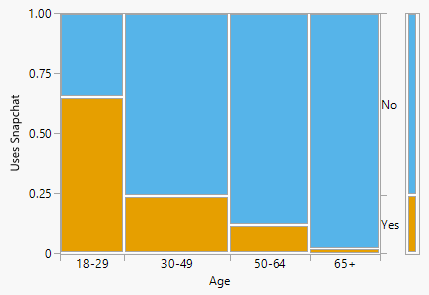
\includegraphics[width=1.43in,height=\textheight,keepaspectratio]{_graphics/snapchat-use-given-age.png}

}

\subcaption{\label{fig-conditional-probability-def2-mosaic-1}Conditioning
on age group}

\end{minipage}%
%
\begin{minipage}{0.50\linewidth}

\centering{

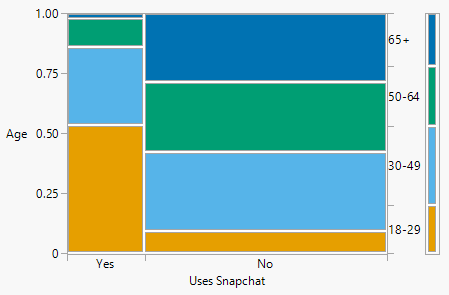
\includegraphics[width=1.5in,height=\textheight,keepaspectratio]{_graphics/snapchat-age-given-use.png}

}

\subcaption{\label{fig-conditional-probability-def2-mosaic-2}Conditioning
on Snapchat use}

\end{minipage}%

\caption{\label{fig-conditional-probability-def2-mosaic}Mosaic plots for
Example~\ref{exm-conditional-probability-def2}}

\end{figure}%

\subsection{Multiplication rule}\label{multiplication-rule}

In Example~\ref{exm-conditional-probability-def2} we were given marginal
probabilities of age groups and conditional probabilities of Snapchat
use given age groups, and we computed joint probabilities. For example:

\begin{itemize}
\tightlist
\item
  20\% \emph{of adults} are age 18-29
\item
  65\% \emph{of adults age 18-29} use Snapchat
\item
  So 13\% \emph{of adults} are age 18-29 and use Snapchat,
  \(0.13 = 0.20\times 0.65\).
\end{itemize}

In fraction terms,

\[
\scriptsize{
\frac{\text{adults age 18-29 who use Snapchat}}{\text{adults}} = \left(\frac{\text{adults age 18-29}}{\text{adults}}\right)\left(\frac{\text{adults age 18-29 who use Snapchat}}{\text{adults age 18-29}}\right)
}
\]

This calculation is an application of the following multiplication rule
which we have already applied intuitively in several examples.

\begin{lemma}[Multiplication
rule]\protect\hypertarget{lem-multiplication-rule}{}\label{lem-multiplication-rule}

The probability that two events \(A\) and \(B\) both occur is

\end{lemma}

\[
\begin{aligned}
\textrm{P}(A \cap B) & = \textrm{P}(A|B)\textrm{P}(B)\\
& = \textrm{P}(B|A)\textrm{P}(A)
\end{aligned}
\]

The multiplication rule is just a rearranging of the definition of the
conditional probability of one event given another. The multiplication
rule says that you should think ``multiply'' when you see ``and''.
However, be careful about \emph{what} you are multiplying: to find a
joint probability you need an unconditional probability and an
appropriate conditional probability. You can condition either on \(A\)
or on \(B\), provided you have the appropriate marginal probability;
often, conditioning one way is easier than the other based on the
available information. Be careful: the multiplication rule does
\emph{not} say that \(\textrm{P}(A\cap B)\) is equal to
\(\textrm{P}(A)\textrm{P}(B)\).

Generically, the multiplication rule says \[
\text{joint} = \text{conditional}\times\text{marginal}
\] We will see several versions of this general relationship in the
remaining chapters.

The multiplication rule is useful in situations where conditional
probabilities are easier to obtain directly than joint probabilities.

\begin{tcolorbox}[enhanced jigsaw, opacityback=0, left=2mm, colframe=quarto-callout-note-color-frame, toprule=.15mm, breakable, colback=white, leftrule=.75mm, arc=.35mm, rightrule=.15mm, bottomrule=.15mm]

\begin{example}[]\protect\hypertarget{exm-card-multiplication-rule}{}\label{exm-card-multiplication-rule}

A standard deck of playing cards has 52 cards, 13 cards (2 through 10,
jack, king, queen, ace) in each of 4 suits (hearts, diamonds, clubs,
spades). Shuffle a deck and deals cards one at a time without
replacement.

\begin{enumerate}
\def\labelenumi{\arabic{enumi}.}
\tightlist
\item
  Compute the probability that the first card dealt is a heart.
\item
  If the first card dealt is a heart, determine the conditional
  probability that the second card is a heart.
\item
  Compute the probability that the first two cards dealt are hearts.
\item
  Compute the probability that the first two cards dealt are hearts and
  the third card dealt is a diamond.
\item
  Shuffle the deck and deal cards one at a time until an ace is dealt,
  and then stop. Compute the probability that more than 4 cards are
  dealt. (Hint: consider the first 4 cards dealt.)
\end{enumerate}

\end{example}

\end{tcolorbox}

\begin{tcolorbox}[enhanced jigsaw, opacityback=0, rightrule=.15mm, coltitle=black, colframe=quarto-callout-tip-color-frame, toprule=.15mm, colbacktitle=quarto-callout-tip-color!10!white, opacitybacktitle=0.6, left=2mm, toptitle=1mm, breakable, title={Solution (click to expand)}, bottomtitle=1mm, colback=white, leftrule=.75mm, titlerule=0mm, arc=.35mm, bottomrule=.15mm]

\begin{refsolution}
\leavevmode

\begin{enumerate}
\def\labelenumi{\arabic{enumi}.}
\tightlist
\item
  If the cards are well shuffled, then any of the cards in the deck is
  equally likely to be the first card dealt. There are 13 hearts out of
  52 cards in the deck, so the probability that the first card is a
  heart is 13/52 = 1/4 = 0.25.
\item
  If the first card dealt is a heart, there are 51 cards left in the
  deck, 12 of which are hearts (and all the remaining cards in the deck
  are equally likely to be the next one drawn). So the conditional
  probability that the second card is a heart given that the first card
  is a heart is 12/51 = 0.235.
\item
  Use the multiplication rule: the probability the both cards are hearts
  is the product of the probability that the first card is a heart and
  the conditional probability that the second card is a heart given that
  the first card is a heart, (13/52)(12/51) = 0.0588. If we imagine
  132600 repetitions (a convenient choice given these fractions), then
  we would expect the first card to be a heart in 33150=132600(13/52)
  repetitions, and among these 33150 repetitions we would expect the
  second card to be a heart in 7800=33150(12/51) repetitions, so the
  proportion of repetitions in which both cards are hearts is
  7800/132600 = 0.0588.
\item
  The third card adds a third ``stage'' but the multiplication rule
  extends naturally. The probability the first two cards dealt are
  hearts and the third card dealt is a diamond is (13/52)(12/51)(13/50)=
  0.0153, the product of:

  \begin{itemize}
  \tightlist
  \item
    13/52, the probability that the first card is a heart,
  \item
    12/51, the conditional probability that the second card is a heart
    given that the first card is a heart, and
  \item
    13/50, the conditional probability that the third card is a diamond
    given that the first two cards are hearts. (If the first two cards
    are hearts, then there are 50 cards remaining in the deck, of which
    13 are diamonds.) Continuing the simulation from the previous part,
    among the 7800 repetitions in which the first two cards are hearts,
    we would expect the third card will be a diamond in 2028 =
    7800(13/50) repetitions, so the proportion of repetitions in which
    the first two cards are hearts and the third is a diamond is
    2028/132600 = 0.0153.
  \end{itemize}
\item
  The key is to recognize that in this scenario more than 4 cards are
  needed to obtain the first ace if and only if the first four cards
  dealt are \emph{not} aces. The probability that the first 4 cards are
  not aces is \((48/52)(47/51)(46/50)(45/49) = 0.719\).
\end{enumerate}

\label{sol-card-multiplication-rule}

\end{refsolution}

\end{tcolorbox}

The multiplication rule extends naturally to more than two events
(though the notation gets messy). For three events, we have

\[
\textrm{P}(A_1 \cap A_2 \cap A_3) = \textrm{P}(A_1)\textrm{P}(A_2|A_1)\textrm{P}(A_3|A_1\cap A_2)
\]

And in general, \[
\textrm{P}(A_1\cap A_2 \cap A_3 \cap A_4 \cap \cdots) = \textrm{P}(A_1)\textrm{P}(A_2|A_1)\textrm{P}(A_3|A_1\cap A_2)\textrm{P}(A_4|A_1\cap A_2 \cap A_4)\cdots
\]

The multiplication rule is useful for computing probabilities of events
that can be broken down into component ``stages'' where conditional
probabilities at each stage are readily available. At each stage,
condition on the information about all previous stages.

\begin{tcolorbox}[enhanced jigsaw, opacityback=0, left=2mm, colframe=quarto-callout-note-color-frame, toprule=.15mm, breakable, colback=white, leftrule=.75mm, arc=.35mm, rightrule=.15mm, bottomrule=.15mm]

\begin{example}[]\protect\hypertarget{exm-birthday}{}\label{exm-birthday}

The \href{https://pudding.cool/2018/04/birthday-paradox/}{birthday
problem} concerns the probability that at least two people in a group of
\(n\) people have the same birthday\footnotemark{}. Ignore multiple
births and February 29 and assume that the other 365 days are all
equally likely\footnotemark{}.

\begin{enumerate}
\def\labelenumi{\arabic{enumi}.}
\tightlist
\item
  If \(n=30\), what do you think the probability that at least two
  people share a birthday is: 0-20\%, 20-40\%, 40-60\%, 60-80\%,
  80-100\%? How large do you think \(n\) needs to be in order for the
  probability that at least two people share a birthday to be larger
  than 0.5? Just make your best guesses before proceeding to
  calculations.
\item
  Now consider \(n=3\) people, labeled 1, 2, and 3. What is the
  probability that persons 1 and 2 have different birthdays?
\item
  What is the probability that persons 1, 2, and 3 all have different
  birthdays \emph{given} that persons 1 and 2 have different birthdays?
\item
  What is the probability that persons 1, 2, and 3 all have different
  birthdays?
\item
  When \(n = 3\), what is the probability that at least two people share
  a birthday?
\item
  Now consider \(n=4\). What is the probability that 4 people all have
  different birthdays?
\item
  When \(n = 4\), what is the probability that at least two people share
  a birthday?
\item
  For \(n=30\), compute the probability that none of the people have the
  same birthday.
\item
  For \(n=30\), compute the probability that at least two people have
  the same birthday.
\item
  Write a clearly worded sentence interpreting the probability in the
  previous part as a long run relative frequency.
\item
  When \(n=30\), how much more likely than not is it for at least two
  people to have the same birthday?
\item
  Provide an expression of the probability for a general \(n\) and find
  the smallest value of \(n\) for which the probability is over 0.5.
  (You can just try different values of \(n\).)
\item
  When \(n=100\) the probability is about 0.9999997. If you are in a
  group of 100 people and no one shares your birthday, should you be
  surprised? Discuss.
\end{enumerate}

\end{example}

\end{tcolorbox}

\footnotetext{You should really check about this
\href{https://pudding.cool/2018/04/birthday-paradox/}{birthday problem
demo from The Pudding}.}

\footnotetext{Which isn't
\href{https://visme.co/blog/most-common-birthday/}{quite}
\href{http://thedailyviz.com/2016/09/17/how-common-is-your-birthday-dailyviz/}{true}.
However, a non-uniform distribution of birthdays only increases the
probability that at least two people have the same birthday. To see
that, think of an extreme case like if everyone were born in September.}

\begin{tcolorbox}[enhanced jigsaw, opacityback=0, rightrule=.15mm, coltitle=black, colframe=quarto-callout-tip-color-frame, toprule=.15mm, colbacktitle=quarto-callout-tip-color!10!white, opacitybacktitle=0.6, left=2mm, toptitle=1mm, breakable, title={Solution (click to expand)}, bottomtitle=1mm, colback=white, leftrule=.75mm, titlerule=0mm, arc=.35mm, bottomrule=.15mm]

\begin{refsolution}
\leavevmode

\begin{enumerate}
\def\labelenumi{\arabic{enumi}.}
\tightlist
\item
  Your guesses are whatever they are. But many people who have never
  encountered this problem before say that the probability is 0-20\%,
  and it takes \(n\) over at least 100 to get to a probability greater
  than 0.5.
\item
  Whatever person 1's birthday is, the probability that person 2 has the
  same birthday\footnotemark{} is 1/365, so the probability that person
  2 has a different birthday than person 1 is 364/365.
\item
  Given that person 1 and person 2 are born on different days, the
  probability that person 3 is also born on a different day is 363/365.
  Notice the importance of the conditioning; if persons 1 and 2 share
  the same birthday, then the probability that person 3 is born on a
  different day is 364/365.
\item
  Use the multiplication rule: \((364/365)(363/365) = 0.992\), the
  probability that all three are born on different days, is the product
  of the probability that persons 1 and 2 are born on different days,
  and the conditional probability that person 3 is also born on a
  different day given that the first two are.
\item
  Exactly one of the following must be true: (1) all 3 people are born
  on different days, or (2) at least two people share a birthday. Use
  the complement rule: when \(n=3\), the probability that at least two
  people share a birthday is \(1-(364/365)(363/365) = 0.008\).
\item
  Now consider \(n=4\). In order for all 4 people to have different
  birthdays, the first three people must have different birthdays and
  the fourth also has to be different from theirs.

  \begin{itemize}
  \tightlist
  \item
    The probability that the first three people have different birthdays
    is \((364/365)(363/365)\) (from a previous part).
  \item
    Given that the first three people have different birthdays, the
    conditional probability that the fourth person's birthday is also
    different is 362/365. Notice the importance of the conditioning; if
    for example, persons 1 and 2 and 3 all shared the same birthday,
    then the probability that person 4 is born on a different day is
    364/365.
  \item
    Using the multiplication rule, the probability that the first three
    people have different birthdays and the fourth is also different
    from theirs is \((364/365)(363/365)(362/365) = 0.983\)
  \end{itemize}
\item
  Exactly one of the following must be true: (1) all 4 people are born
  on different days, or (2) at least two people share a birthday. Use
  the complement rule: when \(n=4\), the probability that at least two
  people share a birthday is \(1-(364/365)(363/365)(362/365) = 0.016\).
\item
  We can use the method for \(n=3\) and \(n=4\). Imagine lining the 30
  people up in some order. Let \(A_2\) be the event that the first two
  people have different birthdays, \(A_3\) be the event that the first
  three people have different birthdays, and so on, until \(A_{30}\),
  the event that all 30 people have different birthdays. Notice
  \(A_{30}\subseteq A_{29} \subseteq \cdots \subseteq A_3 \subseteq A_2\),
  so
  \(\textrm{P}(A_{30}) = \textrm{P}(A_2 \cap A_3 \cap \cdots \cap A_{30})\).

  \begin{itemize}
  \tightlist
  \item
    The first person's birthday can be any one of 365 days. In order for
    the second person's birthday to be different, it needs to be on one
    of the remaining 364 days. So the probability that the second
    person's birthday is different from the first is
    \(\textrm{P}(A_2)=\frac{364}{365}\).
  \item
    Now if the first two people have different birthdays, in order for
    the third person's birthday to be different it must be on one of the
    remaining 363 days. So \(\textrm{P}(A_3|A_2) = \frac{363}{365}\).
    Notice that this is a conditional probability. (If the first two
    people had the same birthday, then the probability that the third
    person's birthday is different would be \(\frac{364}{365}\).)
  \item
    If the first three people have different birthdays, in order for the
    fourth person's birthday to be different it must be on one of the
    remaining 362 days. So
    \(\textrm{P}(A_4|A_2\cap A_3) = \frac{362}{365}\).
  \item
    And so on. If the first 29 people have different birthdays, in order
    for the 30th person's birthday to be different it must be on one of
    the remaining 365-29=336 days. Then using the multiplication rule
    \begin{align*}
    \textrm{P}(A_{30}) & = \textrm{P}(A_{2}\cap A_3 \cap \cdots \cap A_{30})\\
    & = \textrm{P}(A_2)\textrm{P}(A_3|A_2)\textrm{P}(A_4|A_2\cap A_3)\textrm{P}(A_5|A_2\cap A_3 \cap A_4)\cdots \textrm{P}(A_{30}|A_2\cap \cdots \cap A_{29})\\
    & = \left(\frac{364}{365}\right)\left(\frac{363}{365}\right)\left(\frac{362}{365}\right)\left(\frac{361}{365}\right)\cdots \left(\frac{365-30 + 1}{365}\right)\approx 0.294
    \end{align*}\\
  \end{itemize}
\item
  By the complement rule, the probability that at least two people have
  the same birthday is \(1-0.294=0.706\), since either (1) none of the
  people have the same birthday, or (2) at least two of the people have
  the same birthday.
\item
  In about 70\% of \emph{groups of 30 people} at least two people in the
  group will have the same birthday. For example, if Cal Poly classes
  all have 30 students, then in about 70\% of your classes at least two
  people in the class will share a birthday.
\item
  \(0.706 / 0.294 = 2.4.\) In a group of \(n=30\) people it is about 2.4
  times more likely to have at least two people with the same birthday
  than not.
\item
  For a general \(n\), the probability that at least two people have the
  same birthday is \[
  1 - \left(\frac{364}{365}\right)\left(\frac{363}{365}\right)\left(\frac{362}{365}\right)\left(\frac{361}{365}\right)\cdots \left(\frac{365-n + 1}{365}\right)
  \] See Figure~\ref{fig-birthday-function} which plots this probability
  as a function of \(n\). When \(n=23\) this probability is 0.507.
\item
  Maybe, but not because of the 0.999997. 0.999997 is the probability
  that \emph{at least two people} in the group of 100 share a birthday.
  It is NOT the probability that someone shares YOUR birthday. The
  probability that no one shares your birthday is about \(0.76\)---we'll
  see how to compute this later---so it's about 3.1 times more likely
  than not that someone in a group of 100 people shares your birthday.
\end{enumerate}

\label{sol-birthday}

\end{refsolution}

\end{tcolorbox}

\footnotetext{Sometimes students mistake this for \((1/365)^2\), but
\((1/365)^2\) would be the probability that person 1 and person 2 both
have a particular birthday, like the probability that both are born on
January 1. There are \(365^2\) possible (person 1, person 2) birthday
pairs, of which 365 --- (Jan 1, Jan 1), (Jan 2, Jan 2), etc --- result
in the same birthday, so the probability of sharing a birthday is
\(365/365^2 = 1/365\).}

\begin{figure}

\centering{

\pandocbounded{\includegraphics[keepaspectratio]{language-probability_files/figure-pdf/fig-birthday-function-1.png}}

}

\caption{\label{fig-birthday-function}Probability of at least one
birthday match as a function of the number of people in the room in
Example~\ref{exm-birthday}. For 23 people, the probability of at least
one birthday match is 0.507.}

\end{figure}%

That only 23 people are needed to have a better than 50\% chance of a
birthday match is surprising to many people, because 23 doesn't seem
like a lot of people. But when determining if there is a birthday match,
we need to consider every \emph{pair} of people in the group. In a group
of 23 people, there are \(23(22)/2 = 253\) different pairs of people,
and each one of these pairs has a chance of sharing a birthday.

\subsection{Law of total probability}\label{law-of-total-probability}

The law of total probability says that a marginal probability can be
thought of as a weighted average of ``case-by-case'' conditional
probabilities, where the weights are determined by the likelihood or
plausibility of each case.

\begin{tcolorbox}[enhanced jigsaw, opacityback=0, left=2mm, colframe=quarto-callout-note-color-frame, toprule=.15mm, breakable, colback=white, leftrule=.75mm, arc=.35mm, rightrule=.15mm, bottomrule=.15mm]

\begin{example}[]\protect\hypertarget{exm-conditional-probability-def-ltp}{}\label{exm-conditional-probability-def-ltp}

Continuing Example~\ref{exm-conditional-probability-def2}.

\begin{enumerate}
\def\labelenumi{\arabic{enumi}.}
\tightlist
\item
  Donny Don't says: ``The average of the probabilities of using Snapchat
  for each age group---0.65, 0.24, 0.12, and 0.02---is 0.2575. Why isn't
  \(\textrm{P}(C)\), the probability of using Snapchat equal to 0.2575
  (instead of 0.2436)?'' Can you answer Donny's question? (Hint:
  consider an extreme case; for example, if everyone were age 18-29 what
  would \(\textrm{P}(C)\) be?)
\item
  Show how \(\textrm{P}(C) = 0.2436\) can be written as a
  \emph{weighted} average of the values 0.65, 0.24, 0.12, and 0.02.
\item
  Show how \(\textrm{P}(A_1)\) can be written as a \emph{weighted}
  average---what probabilities are being averaged and what are they
  weights?
\end{enumerate}

\end{example}

\end{tcolorbox}

\begin{tcolorbox}[enhanced jigsaw, opacityback=0, rightrule=.15mm, coltitle=black, colframe=quarto-callout-tip-color-frame, toprule=.15mm, colbacktitle=quarto-callout-tip-color!10!white, opacitybacktitle=0.6, left=2mm, toptitle=1mm, breakable, title={Solution (click to expand)}, bottomtitle=1mm, colback=white, leftrule=.75mm, titlerule=0mm, arc=.35mm, bottomrule=.15mm]

\begin{refsolution}
\leavevmode

\begin{enumerate}
\def\labelenumi{\arabic{enumi}.}
\tightlist
\item
  If all adults were age 18-29 then the overall probability of using
  Snapchat would be 0.65; if all adults were age 65+ the overall
  probability of using Snapchat would be 0.02. The overall probability
  of using Snapchat depends on the age group breakdown. The marginal
  probabilities of the age groups differ, partly because the age groups
  cover different numbers of ages.
\item
  We can write our two-way table calculation of \(\textrm{P}(C)\) in
  Example~\ref{exm-conditional-probability-def2} in formulas as
  \begin{align*}
   \textrm{P}(C) & = \textrm{P}(C \cap A_1) + \textrm{P}(C \cap A_2) + \textrm{P}(C \cap A_3) + \textrm{P}(C \cap A_4)\\
   & = \textrm{P}(C|A_1)\textrm{P}(A_1) + \textrm{P}(C|A_2)\textrm{P}(A_2) + \textrm{P}(C|A_3)\textrm{P}(A_3) +\textrm{P}(C|A_4)\textrm{P}(A_4)\\
   & = 0.65\times 0.20 + 0.24\times 0.33 + 0.12 \times 0.25 + 0.02\times 0.22\\
   & = 0.2436
   \end{align*} The above shows that the overall probability of using
  Snapchat, \(\textrm{P}(C) = 0.2436\), is a weighted average of the
  conditional probabilities of using Snapchat for each of the age
  groups---\(\textrm{P}(C|A_1) = 0.65\), \(\textrm{P}(C|A_2) = 0.24\),
  \(\textrm{P}(C|A_3) = 0.12\), \(\textrm{P}(C|A_4) = 0.02\)---where the
  weights are the marginal probabilities of the age groups,
  \(\textrm{P}(A_1) = 0.20\), \(\textrm{P}(A_2) = 0.33\),
  \(\textrm{P}(A_3) = 0.25\), \(\textrm{P}(A_4) = 0.22\).
\item
  Now we break down the probability into two cases, using/not using
  Snapchat. \begin{align*}
   \textrm{P}(A_1) & = \textrm{P}(A_1\cap C) + \textrm{P}(A_1 \cap C^c)\\
   & = \textrm{P}(A_1 | C)\textrm{P}(C) + \textrm{P}(A_1 | C^c)\textrm{P}(C^c)\\
   & = 0.5337\times 0.2436 + 0.0925 \times (1 - 0.2436)\\
   & = 0.20
   \end{align*} The above shows that the overall probability of being
  age 18-29, \(\textrm{P}(A_1) = 0.20\), is a weighted average of the
  conditional probabilities of being age 18-29 for each Snapchat use
  case---\(\textrm{P}(A_1|C) = 0.5337\),
  \(\textrm{P}(A_1|C^c) = 0.0925\)---where the weights are the marginal
  probabilities of the Snapchat use cases, \(\textrm{P}(C) = 0.2436\),
  \(\textrm{P}(C^c) = 1-0.2436 = 0.7564\). Since the overall probability
  of not using Snapchat is about 3 times greater than the overall
  probability of using Snapchat, the conditional probability of being
  age 18-29 given the adult does not use Snapchat (0.0925) gets about 3
  times more weight in the average than the conditional probability of
  being age 18-29 given the adult does uses Snapchat (0.5337). This is
  why the overall probability of being age 18-29 (0.20) is closer to
  0.0925 than to 0.5337.
\end{enumerate}

\label{sol-conditional-probability-def-ltp}

\end{refsolution}

\end{tcolorbox}

The previous example illustrates another version of the law of total
probability.

\begin{lemma}[Law of total
probability]\protect\hypertarget{lem-ltp}{}\label{lem-ltp}

If \(C_1, C_2, C_3\ldots\) are disjoint events with
\(C_1\cup C_2 \cup C_3\cup \cdots =\Omega\), then\footnote{Proof: start
  with Lemma~\ref{lem-ltp1} and use the multiplication rule to write
  \(\textrm{P}(A \cap C_1)=\textrm{P}(A|C_1)\textrm{P}(C_1)\), etc.}

\end{lemma}

\begin{align*}
    \textrm{P}(A) & = \textrm{P}(A |C_1)\textrm{P}(C_1) + \textrm{P}(A | C_2)\textrm{P}(C_2) + \textrm{P}(A | C_3)\textrm{P}(C_3) + \cdots
\end{align*}

The events \(C_1, C_2, C_3, \ldots\), which represent the ``cases'',
form a \emph{partition} of the sample space; each outcome
\(\omega\in\Omega\) lies in exactly one of the \(C_i\). The law of total
probability says that we can interpret the unconditional probability
\(\textrm{P}(A)\) as a probability-weighted average of the case-by-case
conditional probabilities \(\textrm{P}(A|C_i)\) where the weights
\(\textrm{P}(C_i)\) represent the probability of encountering each case.

For an illustration of the law of total probability, consider the mosaic
plots in Figure~\ref{fig-conditional-probability-def2-mosaic}. In
Figure~\ref{fig-conditional-probability-def2-mosaic-1}, the heights of
the orange bars for each age group correspond to the conditional
probabilities of using Snapchat given age group (0.65, 0.24, 0.12,
0.02). The widths of these bars are scaled in proportion to the marginal
probabilities of the age groups; the width of the bar for age 30-49 is
1.65 (0.33/0.20) times wider than the width for age 18-29. The height of
the orange part of the single vertical bar on the right represents the
marginal probability of using Snapchat (0.2436), and this is the
weighted average of the heights of the the other orange bars (the
conditional probabilities of using Snapchat given the age groups), with
the weights given by the widths of the other bars (the marginal
probabilities of the age groups).

The influence of the weighting is even more apparent in the mosaic plot
in Figure~\ref{fig-conditional-probability-def2-mosaic-2}. Since the
marginal probability of not using Snapchat is greater than the marginal
probability of using Snapchat, the marginal probabilities of the age
groups are closer to those for the conditional probabilities of the age
groups given the adult does not use Snapchat than those given that the
adult uses Snapchat.

Conditioning and using the law of probability is an effective strategy
in solving many problems, even when the problem doesn't seem to involve
conditioning. For example, when a problem involves iterations or steps
it is often useful to \emph{condition on the result of the first step}.

\begin{tcolorbox}[enhanced jigsaw, opacityback=0, left=2mm, colframe=quarto-callout-note-color-frame, toprule=.15mm, breakable, colback=white, leftrule=.75mm, arc=.35mm, rightrule=.15mm, bottomrule=.15mm]

\begin{example}[]\protect\hypertarget{exm-lookaway-ltp}{}\label{exm-lookaway-ltp}

You and your friend are playing the
\href{https://fivethirtyeight.com/features/what-are-your-chances-of-winning-the-u-s-open/}{``lookaway
challenge''}.

The game consists of possibly multiple rounds. In the first round, you
point in one of four directions: up, down, left or right. At the exact
same time, your friend also looks in one of those four directions. If
your friend looks in the same direction you're pointing, you win!
Otherwise, you switch roles and the game continues to the next
round---now your friend points in a direction and you try to look away.
As long as no one wins, you keep switching off who points and who looks.
The game ends, and the current ``pointer'' wins, whenever the ``looker''
looks in the same direction as the pointer.

Suppose that each player is equally likely to point/look in each of the
four directions, independently from round to round. What is the
probability that you, starting as the pointer, win the \emph{game}?

\begin{enumerate}
\def\labelenumi{\arabic{enumi}.}
\tightlist
\item
  Why might you expect the probability to not be equal to 0.5?
\item
  If you start as the pointer, what is the probability that you win in
  the first round?
\item
  If \(p\) denotes the probability that the player who starts as the
  pointer wins the game, what is the probability that the player who
  starts as the looker wins the game? (Note: \(p\) is the probability
  that the person who starts as pointer wins the whole game, not just
  the first round.)
\item
  Let \(A\) be the event that the person who starts as the pointer wins
  the game, and \(B\) be the event that the person who starts as the
  pointer wins in the first round. What is \(\textrm{P}(A|B)\)?
\item
  Find a simple expression for \(\textrm{P}(A | B^c)\) in terms of
  \(p\). The key is to consider this question: if the player who starts
  as the pointer does not win in the first round, how does the game
  behave from that point forward?
\item
  Condition on the result of the first round and set up an equation to
  solve for \(p\).
\item
  Interpret the probability from the previous part as a long run
  relative frequency.
\item
  How much more likely is the player who starts as the pointer to win
  than the player who starts as the looker?
\end{enumerate}

\end{example}

\end{tcolorbox}

\begin{tcolorbox}[enhanced jigsaw, opacityback=0, rightrule=.15mm, coltitle=black, colframe=quarto-callout-tip-color-frame, toprule=.15mm, colbacktitle=quarto-callout-tip-color!10!white, opacitybacktitle=0.6, left=2mm, toptitle=1mm, breakable, title={Solution (click to expand)}, bottomtitle=1mm, colback=white, leftrule=.75mm, titlerule=0mm, arc=.35mm, bottomrule=.15mm]

\begin{refsolution}
\leavevmode

\begin{enumerate}
\def\labelenumi{\arabic{enumi}.}
\tightlist
\item
  The player who starts as the pointer has the advantage of going first;
  that player can win the game in the first round, but cannot lose the
  game in the first round. So we might expect the player who starts as
  the pointer to be more likely to win than the player who starts as the
  looker.
\item
  1/4. Whichever direction the pointer points, the probability that the
  looker looks in the same direction is 1/4.Alternatively, if we
  represent an outcome in the first round as a pair (point, look) then
  there are 16 possible equally likely outcomes, of which 4 represent
  pointing and looking in the same direction.
\item
  \(1-p\), since the game keeps going until someone wins.
\item
  \(\textrm{P}(A|B)=1\) since if the person who starts as the pointer
  wins the first round then they win the game.
\item
  The key is to recognize that \emph{if the person who starts as the
  pointer does not win in the first round, it is like the game starts
  over with the roles reversed.} That is, the player who originally
  started as the pointer, having not won the first round, is now
  starting as the looker, and the probability that the player who starts
  as the looker wins the game is \(1-p\). That is,
  \(\textrm{P}(A|B^c) = 1-p\).
\item
  Here is where we use conditioning and the law of total probability. We
  condition on what happens in the first round: either the person who
  starts as the pointer wins the first round and the game ends (event
  \(B\)), or the person who starts as the pointer does not win the the
  first round and the game continues with the other player becoming the
  pointer for the next round (event \(B^c\)). By the law of total
  probability \[
  \textrm{P}(A) = \textrm{P}(A|B)\textrm{P}(B) + \textrm{P}(A|B^c)\textrm{P}(B^c)
  \] From previous parts \(\textrm{P}(A)=p\), \(\textrm{P}(B)=1/4\),
  \(\textrm{P}(B^c)=3/4\), \(\textrm{P}(A|B) = 1\), and
  \(\textrm{P}(A|B^c)=1-p\). Therefore \[
  p = (1)(1/4)+ (1-p)(3/4)
  \] Solve to find \(p=4/7= 0.571\).
\item
  Over many games of the lookaway challenge, the player who starts as
  the pointer wins about 57.1\% of games.
\item
  The player who starts as the pointer is about
  \((4/7)/(3/7) = 4/3= 1.33\) times more likely to win the game than the
  player who starts as the looker.
\end{enumerate}

\label{sol-lookaway-ltp}

\end{refsolution}

\end{tcolorbox}

The game in Example~\ref{exm-lookaway-ltp} could potentially last any
number of rounds (1, 2, 3, \ldots) However, the law of total probability
allowed us to take advantage of the iterative nature of the game, and
consider only one round rather than enumerating all the possibilities of
what might happen over many potential rounds.

\subsection{Conditioning is ``slicing and
renormalizing''}\label{conditioning-is-slicing-and-renormalizing}

\begin{tcolorbox}[enhanced jigsaw, opacityback=0, left=2mm, colframe=quarto-callout-note-color-frame, toprule=.15mm, breakable, colback=white, leftrule=.75mm, arc=.35mm, rightrule=.15mm, bottomrule=.15mm]

\begin{example}[]\protect\hypertarget{exm-conditional-probability-def-slicing}{}\label{exm-conditional-probability-def-slicing}

Continuing Example~\ref{exm-conditional-probability-def2}.

\begin{enumerate}
\def\labelenumi{\arabic{enumi}.}
\tightlist
\item
  How many times more likely is it for an American \emph{adult} to be a
  Snapchat user and age 18-29 than to be:

  \begin{enumerate}
  \def\labelenumii{\alph{enumii}.}
  \tightlist
  \item
    a Snapchat user and age 30-49?
  \item
    a Snapchat user and age 50-64?
  \item
    a Snapchat user and age 65+?
  \end{enumerate}
\item
  How many times more likely is it for an American \emph{adult who uses
  Snapchat} to be age 18-29 than to be:

  \begin{enumerate}
  \def\labelenumii{\alph{enumii}.}
  \tightlist
  \item
    age 30-49?
  \item
    age 50-64?
  \item
    age 65+?
  \end{enumerate}
\item
  What do you notice about the answers to the two previous parts?
\end{enumerate}

\end{example}

\end{tcolorbox}

\begin{tcolorbox}[enhanced jigsaw, opacityback=0, rightrule=.15mm, coltitle=black, colframe=quarto-callout-tip-color-frame, toprule=.15mm, colbacktitle=quarto-callout-tip-color!10!white, opacitybacktitle=0.6, left=2mm, toptitle=1mm, breakable, title={Solution (click to expand)}, bottomtitle=1mm, colback=white, leftrule=.75mm, titlerule=0mm, arc=.35mm, bottomrule=.15mm]

\begin{refsolution}
\leavevmode

\begin{enumerate}
\def\labelenumi{\arabic{enumi}.}
\tightlist
\item
  Use the joint probabilities we computed in
  Example~\ref{exm-conditional-probability-def2}; see the ``uses
  Snapchat'' column of the two-way table in the solution to part 4. The
  joint probability that an American \emph{adult} is a Snapchat user and
  age 18-29 is:

  \begin{enumerate}
  \def\labelenumii{\alph{enumii}.}
  \tightlist
  \item
    \(\frac{0.1300}{0.0792} = 1.64\) times greater than the joint
    probability that an American \emph{adult} is a Snapchat user and age
    30-49
  \item
    \(\frac{0.1300}{0.0300} = 4.33\) times greater than the joint
    probability that an American \emph{adult} is a Snapchat user and age
    50-64
  \item
    \(\frac{0.1300}{0.0044} = 29.55\) times greater than the joint
    probability that an American \emph{adult} is a Snapchat user and age
    65+
  \end{enumerate}
\item
  Use the conditional probabilities we computed in
  Example~\ref{exm-conditional-probability-def2}; see the solution to
  part 7. The conditional probability that an American adult is age
  18-29 \emph{given that they use Snapchat} is:

  \begin{enumerate}
  \def\labelenumii{\alph{enumii}.}
  \tightlist
  \item
    \(\frac{0.5337}{0.3251} = \frac{0.1300/0.2436}{0.0792/0.2436} = 1.64\)
    times greater than the conditional probability that an American
    adult is age 30-49 \emph{given that they use Snapchat}.
  \item
    \(\frac{0.5337}{0.1232} = \frac{0.1300/0.2436}{0.0300/0.2436}= 4.33\)
    times greater than the conditional probability that an American
    adult is age 50-64 \emph{given that they use Snapchat}.
  \item
    \(\frac{0.5337}{0.0181} = \frac{0.1300/0.2436}{0.0044/0.2436} = 29.55\)
    times greater than The conditional probability that an American
    adult is age 65+ \emph{given that they use Snapchat}.
  \end{enumerate}
\item
  The ratios are the same\footnotemark{}! Conditioning on using Snapchat
  zooms in on the ``slice'' of adults who use Snapchat in the two-way
  table of joint probabilities. The ratios within this slice are
  determined by the joint probabilities for adults, as in part 1. The
  conditional probabilities given Snapchat use that we used to compute
  ratios in part 2 are simply rescaled versions of the joint
  probabilities for the ``use Snapchat slice''; rescaled so that the
  slice represents 100\% of the probability given that the adult uses
  Snapchat.
\end{enumerate}

\label{sol-conditional-probability-def-slicing}

\end{refsolution}

\end{tcolorbox}

\footnotetext{They should be exactly the same; any differences are due
to rounding.}

The process of conditioning can be thought of as \textbf{``slicing and
renormalizing''.}

\begin{enumerate}
\def\labelenumi{\arabic{enumi}.}
\tightlist
\item
  Extract the ``slice'' corresponding to the event being conditioned on
  (and discard the rest). For example, a slice might correspond to a
  particular row or column of a two-way table, or a section of a plot.\\
\item
  ``Renormalize'' the values in the slice so that corresponding
  probabilities add up to 1.
\end{enumerate}

Slicing determines \emph{shape}; renormalizing determines \emph{scale}.
Slicing determines relative probabilities; renormalizing just makes sure
they add up to 1.

Consider the mosaic plot in
Figure~\ref{fig-conditional-probability-def2-mosaic-2}, where the areas
of rectangles represent joint probabilities. The areas of the rectangles
in the ``uses Snapchat'' column represent the joint probabilities we
used in part 1 of Example~\ref{exm-conditional-probability-def2}.
Imagine taking the rectangles in this column and unstacking them to make
a bar plot with heights determined by the joint probabilities of being
in each age group and using Snapchat, as in
Figure~\ref{fig-conditional-probability-def-slicing-1}. The ``slice''
determines the shape of the bar plot: The bar for age 18-29 is 1.64
times higher than the bar for age 30-49, 4.33 times higher than the bar
for age 50-64, and 29.55 times higher than the bar for age 65+.

Summing the joint probabilities in
Figure~\ref{fig-conditional-probability-def-slicing-1} over the age
groups yields 0.2436, the marginal probability that an adult uses
Snapchat. Given that the adult uses Snapchat, we want the conditional
probabilities of the age groups to sum to 1. Thus we ``renormalize'' the
joint probabilities on the vertical axis---by dividing each by
0.2436---so that they sum to 1 to obtain the conditional probabilities
of each age group given that the adult uses Snapchat, displayed in
Figure~\ref{fig-conditional-probability-def-slicing-2}. Renormalizing
only changes the absolute scale of the plot; compare the values on the
vertical axes in Figure~\ref{fig-conditional-probability-def-slicing},
which correspond to joint probabilities on the left and conditional
probabilities on the right. Both plots have the same relative shape: the
bar for age 18-29 is 1.64 times higher than the bar for age 30-49, 4.33
times higher than the bar for age 50-64, and 29.55 times higher than the
bar for age 65+.

\begin{figure}

\begin{minipage}{0.50\linewidth}

\centering{

\pandocbounded{\includegraphics[keepaspectratio]{language-probability_files/figure-pdf/fig-conditional-probability-def-slicing-1.png}}

}

\subcaption{\label{fig-conditional-probability-def-slicing-1}Joint
probability of each age group and Snapchat use for the uses Snapchat
slice}

\end{minipage}%
%
\begin{minipage}{0.50\linewidth}

\centering{

\pandocbounded{\includegraphics[keepaspectratio]{language-probability_files/figure-pdf/fig-conditional-probability-def-slicing-2.png}}

}

\subcaption{\label{fig-conditional-probability-def-slicing-2}Renormalized,
conditional probability of each age group given that the adult uses
Snapchat.}

\end{minipage}%

\caption{\label{fig-conditional-probability-def-slicing}Illustration of
slicing and renormalizing for
Example~\ref{exm-conditional-probability-def-slicing}}

\end{figure}%

\begin{tcolorbox}[enhanced jigsaw, opacityback=0, left=2mm, colframe=quarto-callout-note-color-frame, toprule=.15mm, breakable, colback=white, leftrule=.75mm, arc=.35mm, rightrule=.15mm, bottomrule=.15mm]

\begin{example}[]\protect\hypertarget{exm-venn-conditional}{}\label{exm-venn-conditional}

Each of the three Venn diagrams below represents a sample space with 16
equally likely outcomes. Let \(A\) be the yellow \texttt{/} event, \(B\)
the blue \texttt{\textbackslash{}} event, and their intersection
\(A\cap B\) the green \(\times\) event. Suppose that areas represent
probabilities, so that for example \(\textrm{P}(A) = 4/16\).

Find \(\textrm{P}(A|B)\) for each of the scenarios. Be sure to indicate
what represents the ``slice'' in each scenario.

\end{example}

\end{tcolorbox}

\begin{figure}

\centering{

\includegraphics[width=4.18in,height=\textheight,keepaspectratio]{_graphics/venn-conditional.png}

}

\caption{\label{fig-venn-conditional-plot}Three sample spaces with 16
equally outcomes}

\end{figure}%

\begin{tcolorbox}[enhanced jigsaw, opacityback=0, rightrule=.15mm, coltitle=black, colframe=quarto-callout-tip-color-frame, toprule=.15mm, colbacktitle=quarto-callout-tip-color!10!white, opacitybacktitle=0.6, left=2mm, toptitle=1mm, breakable, title={Solution (click to expand)}, bottomtitle=1mm, colback=white, leftrule=.75mm, titlerule=0mm, arc=.35mm, bottomrule=.15mm]

\begin{refsolution}
In each case we're conditioning on event \(B\), so the slice represents
the 4 blue outcomes. Imagine zooming in on the blue (including green)
area of each plot: remove the slice with the 4 blue outcomes (and erase
the rest) and then magnify (renormalize) the slice so that it is the
size of the original rectangle.

\begin{enumerate}
\def\labelenumi{\arabic{enumi}.}
\tightlist
\item
  Left: \(\textrm{P}(A|B)=0\). After conditioning on \(B\), there are
  now 4 equally likely outcomes, of which none satisfy \(A\).
\item
  Middle: \(\textrm{P}(A|B) = 2/4=1/2\). After conditioning on \(B\),
  there are now 4 equally likely outcomes, of which 2 satisfy \(A\). The
  green part represents 1/2 of the area of the blue slice.
\item
  Right: \(\textrm{P}(A|B) = 1/4\). After conditioning on \(B\), there
  are now 4 equally likely outcomes, of which 1 satisfies \(A\). The
  green part represents 1/4 of the area of the blue slice.
\end{enumerate}

\label{sol-venn-condition}

\end{refsolution}

\end{tcolorbox}

We will see that ``slicing and renormalizing'' is a helpful way to
conceptualize conditioning, especially when dealing with conditional
distributions of random variables.

\subsection{Bayes rule}\label{bayes-rule}

Bayes' rule describes how to update uncertainty in light of new
information, evidence, or data. We'll introduce it in the context of
two-way tables.

\begin{tcolorbox}[enhanced jigsaw, opacityback=0, left=2mm, colframe=quarto-callout-note-color-frame, toprule=.15mm, breakable, colback=white, leftrule=.75mm, arc=.35mm, rightrule=.15mm, bottomrule=.15mm]

\begin{example}[]\protect\hypertarget{exm-bayes-rule-iterative-twoway}{}\label{exm-bayes-rule-iterative-twoway}

A
\href{https://www.pewresearch.org/science/2019/03/28/what-americans-know-about-science/}{recent
survey} of American adults asked: ``Based on what you have heard or
read, which of the following two statements best describes the
scientific method?''

\begin{itemize}
\tightlist
\item
  70\% selected ``The scientific method produces findings meant to be
  continually tested and updated over time''. (We'll call this the
  ``iterative'' opinion.)
\item
  14\% selected ``The scientific method identifies unchanging core
  principles and truths''. (We'll call this the ``unchanging'' opinion).
\item
  16\% were not sure which of the two statements was best.
\end{itemize}

How does the response to this question change based on education level?
Suppose education level is classified as: high school or less (HS), some
college but no Bachelor's degree (college), Bachelor's degree
(Bachelor's), or postgraduate degree (postgraduate). The education
breakdown is

\begin{itemize}
\tightlist
\item
  Among those who agree with ``iterative'': 31.3\% HS, 27.6\% college,
  22.9\% Bachelor's, and 18.2\% postgraduate.
\item
  Among those who agree with ``unchanging'': 38.6\% HS, 31.4\% college,
  19.7\% Bachelor's, and 10.3\% postgraduate.
\item
  Among those ``not sure'': 57.3\% HS, 27.2\% college, 9.7\% Bachelor's,
  and 5.8\% postgraduate
\end{itemize}

\begin{enumerate}
\def\labelenumi{\arabic{enumi}.}
\tightlist
\item
  Use the information to construct an appropriate two-way table.
\item
  Overall what percentage of adults have a postgraduate degree? How is
  this related to the values 18.2\%, 10.3\%, and 5.8\%?
\item
  What percent of those with a postgraduate degree agree that the
  scientific method is ``iterative''? How is this related to the values
  provided?
\end{enumerate}

\end{example}

\end{tcolorbox}

\begin{tcolorbox}[enhanced jigsaw, opacityback=0, rightrule=.15mm, coltitle=black, colframe=quarto-callout-tip-color-frame, toprule=.15mm, colbacktitle=quarto-callout-tip-color!10!white, opacitybacktitle=0.6, left=2mm, toptitle=1mm, breakable, title={Solution (click to expand)}, bottomtitle=1mm, colback=white, leftrule=.75mm, titlerule=0mm, arc=.35mm, bottomrule=.15mm]

\begin{refsolution}
\leavevmode

\begin{enumerate}
\def\labelenumi{\arabic{enumi}.}
\tightlist
\item
  Suppose there are 100000 hypothetical American adults. Of these
  100000, \(100000\times 0.7 = 70000\) agree with the ``iterative''
  statement. Of the 70000 who agree with the ``iterative'' statement,
  \(70000\times 0.182 = 12740\) also have a postgraduate degree.
  Continue in this way to complete
  Table~\ref{tbl-bayes-rule-iterative-twoway}
\item
  Overall 15.11\% of adults have a postgraduate degree (15110/100000 in
  the table). The overall percentage is a weighted average of the three
  percentages; 18.2\% gets the most weight in the average because the
  ``iterative'' statement has the highest percentage of people that
  agree with it compared to ``unchanging'' and ``not sure''. \[
  0.1511 = (0.70)(0.182) + (0.14)(0.103) + (0.16)(0.058)  
  \]
\item
  Of the 15110 who have a postgraduate degree 12740 agree with the
  ``iterative'' statement, and \(12740/15110 = 0.843\). 84.3\% of those
  with a graduate degree agree that the scientific method is
  ``iterative''. The value 0.843 is equal to the product of (1) 0.70,
  the overall proportion who agree with the ``iterative'' statement, and
  (2) 0.182, the proportion of those who agree with the ``iterative''
  statement that have a postgraduate degree; divided by 0.1511, the
  overall proportion who have a postgraduate degree. \[
  0.843 = \frac{0.182 \times 0.70}{0.1511} 
  \]
\end{enumerate}

\label{sol-bayes-rule-iterative-twoway}

\end{refsolution}

\end{tcolorbox}

\begin{table}

\caption{\label{tbl-bayes-rule-iterative-twoway}Two-way table for
Example~\ref{exm-bayes-rule-iterative-twoway}}

\centering{

\centering
\begin{tabular}[t]{l|r|r|r|r|r}
\hline
hypothesis & HS & College & Bachelors & Postgrad & Total\\
\hline
iterative & 21910 & 19320 & 16030 & 12740 & 70000\\
\hline
unchanging & 5404 & 4396 & 2758 & 1442 & 14000\\
\hline
not sure & 9168 & 4352 & 1552 & 928 & 16000\\
\hline
Total & 36482 & 28068 & 20340 & 15110 & 100000\\
\hline
\end{tabular}

}

\end{table}%

\begin{lemma}[Bayes rule for
events]\protect\hypertarget{lem-bayes-rule}{}\label{lem-bayes-rule}

Bayes' rule for events\footnote{This section only covers Bayes' rule for
  events. We'll see Bayes' rule for distributions of random variables
  later. But the ideas are analogous.} specifies how a \emph{prior
probability} \(P(H)\) of event \(H\) is updated in response to the
evidence \(E\) to obtain the \emph{posterior probability} \(P(H|E)\). \[
P(H|E) = \frac{P(E|H)P(H)}{P(E)}
\]

\end{lemma}

\begin{itemize}
\tightlist
\item
  Event \(H\) represents a particular hypothesis\footnote{We're using
    ``hypothesis'' in the sense of a general scientific hypothesis, not
    necessarily a statistical null or alternative hypothesis.} (or model
  or case)
\item
  Event \(E\) represents observed evidence (or data or information)
\item
  \(P(H)\) is the unconditional or \textbf{prior probability} of \(H\)
  (prior to observing evidence \(E\))
\item
  \(P(H|E)\) is the conditional or \textbf{posterior probability} of
  \(H\) after observing evidence \(E\).
\item
  \(P(E|H)\) is the \textbf{likelihood} of evidence \(E\) given
  hypothesis (or model or case) \(H\)
\end{itemize}

\begin{tcolorbox}[enhanced jigsaw, opacityback=0, left=2mm, colframe=quarto-callout-note-color-frame, toprule=.15mm, breakable, colback=white, leftrule=.75mm, arc=.35mm, rightrule=.15mm, bottomrule=.15mm]

\begin{example}[]\protect\hypertarget{exm-bayes-rule-iterative-bayestable}{}\label{exm-bayes-rule-iterative-bayestable}

Continuing Example~\ref{exm-bayes-rule-iterative-twoway}. Randomly
select an American adult.

\begin{enumerate}
\def\labelenumi{\arabic{enumi}.}
\tightlist
\item
  Consider the conditional probability that a randomly selected American
  adult agrees that the scientific method is ``iterative'' given that
  they have a postgraduate degree. Identify the hypothesis, prior
  probability, evidence, likelihood, and posterior probability, and use
  Bayes' rule to compute the posterior probability.
\item
  Compute the conditional probability that a randomly selected American
  adult with a postgraduate degree agrees that the scientific method is
  ``unchanging''.
\item
  Compute the conditional probability that a randomly selected American
  adult with a postgraduate degree is not sure about which statement is
  best.
\item
  How many times more likely is it for an \emph{American adult} to have
  a postgraduate degree and agree with the ``iterative'' statement than
  to have a postgraduate degree and agree with the ``unchanging''
  statement?
\item
  How many times more likely is it for an \emph{American adult with a
  postgraduate degree} to agree with the ``iterative'' statement than to
  agree with the ``unchanging'' statement?
\item
  What do you notice about the answers to the two previous parts?
\item
  How many times more likely is it for an \emph{American adult} to agree
  with the ``iterative'' statement than to agree with the ``unchanging''
  statement?
\item
  How many times more likely is it for an American adult to have a
  postgraduate degree when the adult agrees with the ``iterative''
  statement than when the adult agree with the ``unchanging'' statement?
\item
  How many times more likely is it for an \emph{American adult with a
  postgraduate degree} to agree with the ``iterative'' statement than to
  agree with the ``unchanging'' statement?
\item
  How are the values in the three previous parts related?
\end{enumerate}

\end{example}

\end{tcolorbox}

\begin{tcolorbox}[enhanced jigsaw, opacityback=0, rightrule=.15mm, coltitle=black, colframe=quarto-callout-tip-color-frame, toprule=.15mm, colbacktitle=quarto-callout-tip-color!10!white, opacitybacktitle=0.6, left=2mm, toptitle=1mm, breakable, title={Solution (click to expand)}, bottomtitle=1mm, colback=white, leftrule=.75mm, titlerule=0mm, arc=.35mm, bottomrule=.15mm]

\begin{refsolution}
\leavevmode

\begin{enumerate}
\def\labelenumi{\arabic{enumi}.}
\tightlist
\item
  This is essentially the same question as the last part of
  Example~\ref{exm-bayes-rule-iterative-twoway}, just with different
  terminology.

  \begin{itemize}
  \tightlist
  \item
    The hypothesis is \(H_1\), the event that the randomly selected
    adult agrees with the ``iterative'' statement.
  \item
    The prior probability is \(\textrm{P}(H_1) = 0.70\), the overall or
    unconditional probability that a randomly selected American adult
    agrees with the ``iterative'' statement.
  \item
    The given ``evidence'' \(E\) is the event that the randomly selected
    adult has a postgraduate degree. The marginal probability of the
    evidence is \(\textrm{P}(E)=0.1511\), which can be obtained by the
    law of total probability as in
    Example~\ref{exm-bayes-rule-iterative-twoway}.
  \item
    The likelihood is \(\textrm{P}(E | H_1) = 0.182\), the conditional
    probability that the adult has a postgraduate degree (the evidence)
    given that the adult agrees with the ``iterative'' statement (the
    hypothesis).
  \item
    The posterior probability is \(\textrm{P}(H_1 |E)=0.843\), the
    conditional probability that a randomly selected American adult
    agrees that the scientific method is ``iterative'' given that they
    have a postgraduate degree. By Bayes rule \[
    \textrm{P}(H_1 | E) = \frac{\textrm{P}(E | H_1) \textrm{P}(H_1)}{\textrm{P}(E)} = \frac{0.182 \times 0.70}{0.1511} = 0.843
    \]
  \end{itemize}
\item
  Let \(H_2\) be the event that the randomly selected adult agrees with
  the ``unchanging'' statement; the prior probability is
  \(\textrm{P}(H_2) = 0.14\). The evidence \(E\) is still ``postgraduate
  degree'' but now the likelihood of this evidence is
  \(\textrm{P}(E | H_2) = 0.103\) under the ``unchanging'' hypothesis.
  The conditional probability that a randomly selected adult with a
  postgraduate degree agrees that the scientific method is
  ``unchanging'' is \[
  \textrm{P}(H_2 | E) = \frac{\textrm{P}(E | H_2) \textrm{P}(H_2)}{\textrm{P}(E)} = \frac{0.103 \times 0.14}{0.1511} = 0.095
  \]
\item
  Let \(H_3\) be the event that the randomly selected adult is ``not
  sure''; the prior probability is \(\textrm{P}(H_3) = 0.16\). The
  evidence \(E\) is still ``postgraduate degree'' but now the likelihood
  of this evidence is \(\textrm{P}(E | H_3) = 0.058\) under the ``not
  sure'' hypothesis. The conditional probability that a randomly
  selected adult with a postgraduate degree is ``not sure'' is \[
  \textrm{P}(H_3 | E) = \frac{\textrm{P}(E | H_3) \textrm{P}(H_3)}{\textrm{P}(E)} = \frac{0.058 \times 0.16}{0.1511} = 0.061
  \]
\item
  The probability that an \emph{American adult} has a postgraduate
  degree and agrees with the ``iterative'' statement is
  \(\textrm{P}(E \cap H_1) = \textrm{P}(E|H_1)\textrm{P}(H_1) = 0.182\times 0.70 = 0.1274\).
  The probability that an \emph{American adult} has a postgraduate
  degree and agrees with the ``unchanging'' statement is
  \(\textrm{P}(E \cap H_2) = \textrm{P}(E|H_2)\textrm{P}(H_2) = 0.103\times 0.14 = 0.01442\).
  Since \[
  \frac{\textrm{P}(E \cap H_1)}{\textrm{P}(E \cap H_2)} = \frac{0.182\times 0.70}{0.103\times 0.14} = \frac{0.1274}{0.01442} = 8.835
  \] an \emph{American adult} is 8.835 times more likely to have a
  postgraduate degree and agree with the ``iterative'' statement than to
  have a postgraduate degree and agree with the ``unchanging''
  statement.
\item
  The conditional probability that an \emph{American adult with a
  postgraduate degree} agrees with the ``iterative'' statement is
  \(\textrm{P}(H_1 | E) = \textrm{P}(E|H_1)\textrm{P}(H_1)/\textrm{P}(E) = 0.182\times 0.70/0.1511 = 0.843\).
  The conditional probability that an \emph{American adult with a
  postgraduate degree} agrees with the ``unchanging'' statement is
  \(\textrm{P}(H_2|E) = \textrm{P}(E|H_2)\textrm{P}(H_2)/\textrm{P}(E) = 0.103\times 0.14/0.1511 = 0.09543\).
  Since \[
  \frac{\textrm{P}(H_1 | E)}{\textrm{P}(H_2 | E)} = \frac{0.182\times 0.70/0.1511}{0.103\times 0.14/0.1511} = \frac{0.84315}{0.09543} = 8.835
  \] an \emph{American adult with a postgraduate degree} is 8.835 times
  more likely to agree with the ``iterative'' statement than to agree
  with the ``unchanging'' statement.
\item
  The ratios are the same! Conditioning on having a postgraduate degree
  just ``slices'' out the Americans who have a postgraduate degree. The
  ratios are determined by the overall probabilities for Americans. The
  conditional probabilities, given postgraduate degree, simply rescale
  the probabilities for Americans who have a postgraduate degree to add
  up to 1 (by dividing by 0.1511).
\item
  This is a ratio of prior probabilities: 0.70 / 0.14 = 5. An
  \emph{American adult} is 5 times more likely to agree with the
  ``iterative'' statement than to agree with the ``unchanging''
  statement.
\item
  This is a ratio of likelihoods: 0.182 / 0.103 = 1.767. An American
  adult is 1.767 times more likely to have a postgraduate degree when
  the adult agrees with the iterative statement than when the adult
  agree with the unchanging statement.
\item
  This is a ratio of posterior probabilities: 0.8432 / 0.0954 = 8.835.
  An \emph{American adult with a postgraduate degree} is 8.835 times
  more likely to agree with the ``iterative'' statement than to agree
  with the ``unchanging'' statement.
\item
  The ratio of the posterior probabilities is equal to the product of
  the ratio of the prior probabilities and the ratio of the likelihoods:
  \(8.835 = 5 \times 1.767\). \emph{The posterior is proportional to the
  product of prior and likelihood.}
\end{enumerate}

\label{sol-bayes-rule-iterative-bayestable}

\end{refsolution}

\end{tcolorbox}

Bayes rule is often used when there are multiple hypotheses or cases.
Suppose \(H_1,H_2, \ldots\) is a series of distinct hypotheses which
together account for all possibilities, and \(E\) is any event
(evidence). Then Bayes' rule implies that the posterior probability of
any particular hypothesis \(H_j\) satisfies \[
\textrm{P}(H_j |E) = \frac{\textrm{P}(E|H_j)\textrm{P}(H_j)}{\textrm{P}(E)}
\]

The marginal probability of the evidence, \(\textrm{P}(E)\), in the
denominator can be calculated using the law of total probability \[
\textrm{P}(E) = \textrm{P}(E|H_1) \textrm{P}(H_1) + \textrm{P}(E|H_2) \textrm{P}(H_2) + \textrm{P}(E|H_3) \textrm{P}(H_3) + \cdots
\] Since \(\textrm{P}(E)\) is the sum of the terms
\(\textrm{P}(E|H_j)\textrm{P}(H_j)\) over all the hypotheses, Bayes rule
implies that \(\textrm{P}(H_j |E)\) is \emph{proportional to\footnote{The
  symbol \(\propto\) means ``is proportional to''.}}
\(\textrm{P}(E|H_j)\textrm{P}(H_j)\) \begin{align*}
\textrm{P}(H_j |E) & = \frac{\textrm{P}(E|H_j)\textrm{P}(H_j)}{\textrm{P}(E)}\\
\textrm{P}(H_j |E) & \propto \textrm{P}(E|H_j)\textrm{P}(H_j)
\end{align*}

\textbf{In short, Bayes' rule says that a posterior probability of a
hypothesis is proportional to the product of the prior probability of
the hypothesis and the likelihood of the evidence if the hypothesis were
true.}

\[
\textbf{posterior} \propto \textbf{prior} \times \textbf{likelihood}
\]

Bayes rule calculations are often organized in a \textbf{Bayes' table}
like Table~\ref{tbl-bayes-rule-iterative-bayestable} which illustrates
``posterior is proportional to likelihood times prior''. The table has
one row for each hypothesis and columns for

\begin{itemize}
\tightlist
\item
  prior probability: column sum is 1
\item
  likelihood of the evidence given each hypothesis

  \begin{itemize}
  \tightlist
  \item
    likelihood depends on the evidence; if the evidence changes, the
    likelihood column changes
  \item
    the sum of the likelihood column is a meaningless number and can be
    any value
  \end{itemize}
\item
  product of prior and likelihood: column sum is the marginal
  probability of the evidence
\item
  posterior probability: column sum is 1
\end{itemize}

\begin{table}

\caption{\label{tbl-bayes-rule-iterative-bayestable}Bayes table
representation of the posterior probabilities of each opinion about the
scientific method (the hypotheses) given a postgraduate degree (the
evidence) in Example~\ref{exm-bayes-rule-iterative-bayestable}}

\centering{

\centering
\begin{tabular}[t]{l|r|r|r|r}
\hline
hypothesis & prior & likelihood & product & posterior\\
\hline
iterative & 0.70 & 0.182 & 0.1274 & 0.8432\\
\hline
unchanging & 0.14 & 0.103 & 0.0144 & 0.0954\\
\hline
not sure & 0.16 & 0.058 & 0.0093 & 0.0614\\
\hline
Total & 1.00 & 0.343 & 0.1511 & 1.0000\\
\hline
\end{tabular}

}

\end{table}%

The likelihood column in a Bayes table depends on the evidence. In
Table~\ref{tbl-bayes-rule-iterative-bayestable} the evidence is that the
American has a postgraduate degree; the likelihood column contains the
probability of the same event, \(E\) = ``the American has a postgraduate
degree'', under each of the distinct hypotheses:

\begin{itemize}
\tightlist
\item
  \(\textrm{P}(E |H_1) = 0.182\), given the American agrees with the
  ``iterative'' statement
\item
  \(\textrm{P}(E |H_2) = 0.103\), given the American agrees with the
  ``unchanging'' statement
\item
  \(\textrm{P}(E |H_3) = 0.058\), given the American is ``not sure''
\end{itemize}

Since each of these probabilities is computed under a different case,
these values do not need to add up to anything in particular. The sum of
the likelihoods is meaningless.

The ``product'' column contains the product of the values in the prior
and likelihood columns. In
Table~\ref{tbl-bayes-rule-iterative-bayestable} the product of prior and
likelihood for ``iterative'' (0.1274) is 8.835 (0.1274/0.0144) times
higher than the product of prior and likelihood for ``unchanging''
(0.0144). Therefore, Bayes rule implies that the conditional probability
that an American with a postgraduate degree agrees with ``iterative''
should be 8.835 times higher than the conditional probability that an
American with a postgraduate degree agrees with ``unchanging''.
Similarly, the conditional probability that an American with a
postgraduate degree agrees with ``iterative'' should be
\(0.1274 / 0.0093 = 13.73\) times higher than the conditional
probability that an American with a postgraduate degree is ``not sure'',
and the conditional probability that an American with a postgraduate
degree agrees with ``unchanging'' should be \(0.0144 / 0.0093 = 1.55\)
times higher than the conditional probability that an American with a
postgraduate degree is ``not sure''. The last column just translates
these relative relationships into probabilities that sum to 1.

The sum of the ``product'' column is \(\textrm{P}(E)\), the marginal
probability of the evidence or ``average likelihood''. The sum of the
product column represents the result of the law of total probability
calculation. However, for the purposes of determining the posterior
probabilities, it isn't really important what \(P(E)\) is. Rather, it is
the \emph{ratio} of the values in the ``product'' column that determine
the posterior probabilities. \(\textrm{P}(E)\) is whatever it needs to
be to ensure that the posterior probabilities sum to 1 while maintaining
the proper ratios.

Bayes rule is just another application of conditioning as ``slicing and
renormalizing''.

\begin{itemize}
\tightlist
\item
  Extract the ``slice'' corresponding to the event being conditioned on
  (and discard the rest). For example, a slice might correspond to a
  particular row or column of a two-way table.\\
\item
  ``Renormalize'' the values in the slice so that corresponding
  probabilities add up to 1.
\end{itemize}

In Bayes rule, the product of prior and likelihood determines the shape
of the slice. Slicing determines relative probabilities; renormalizing
just makes sure they ``add up'' to 1 while maintaining the proper
ratios.

\begin{tcolorbox}[enhanced jigsaw, opacityback=0, left=2mm, colframe=quarto-callout-note-color-frame, toprule=.15mm, breakable, colback=white, leftrule=.75mm, arc=.35mm, rightrule=.15mm, bottomrule=.15mm]

\begin{example}[]\protect\hypertarget{exm-bayes-rule-iterative-bayestable2}{}\label{exm-bayes-rule-iterative-bayestable2}

Continuing Example~\ref{exm-bayes-rule-iterative-twoway}. Randomly
select an American adult. Now suppose we want to compute the posterior
probabilities for an American adult's perception of the scientific
method given that the randomly selected American adult has some college
but no Bachelor's degree (``College'').

\begin{enumerate}
\def\labelenumi{\arabic{enumi}.}
\tightlist
\item
  Before computing, make an educated guess for the posterior
  probabilities. In particular, will the changes from prior to posterior
  be more or less extreme given the American has some college but no
  Bachelor's degree than when given the American has a postgraduate
  degree? Why?
\item
  Construct a Bayes table and compute the posterior probabilities.
  Compare to the posterior probabilities given postgraduate degree from
  the previous examples.
\end{enumerate}

\end{example}

\end{tcolorbox}

\begin{tcolorbox}[enhanced jigsaw, opacityback=0, rightrule=.15mm, coltitle=black, colframe=quarto-callout-tip-color-frame, toprule=.15mm, colbacktitle=quarto-callout-tip-color!10!white, opacitybacktitle=0.6, left=2mm, toptitle=1mm, breakable, title={Solution (click to expand)}, bottomtitle=1mm, colback=white, leftrule=.75mm, titlerule=0mm, arc=.35mm, bottomrule=.15mm]

\begin{refsolution}
\leavevmode

\begin{enumerate}
\def\labelenumi{\arabic{enumi}.}
\tightlist
\item
  We start with the same prior probabilities as before: 0.70 for
  iterative, 0.14 for unchanging, 0.16 for not sure. Now the evidence is
  that the American has some college but no Bachelor's degree. The
  likelihood of the evidence (``college'') is 0.276 under the iterative
  hypothesis, 0.314 under the unchanging hypothesis, and 0.272 under the
  not sure hypothesis. The likelihood of the evidence does not change as
  much across the different hypotheses when the evidence is ``college''
  than when the evidence was ``postgraduate degree''. Therefore, the
  changes from prior to posterior should be less extreme when the
  evidence is ``college'' than when the evidence was ``postgraduate
  degree''. Furthermore, since the likelihood doesn't vary much across
  hypotheses when the evidence is ``college'' we expect the posterior
  probabilities to be close to the prior probabilities.
\item
  See Table~\ref{tbl-bayes-rule-iterative-bayestable2} As expected, the
  posterior probabilities are closer to the prior probabilities when the
  evidence is ``college'' than when the evidence is ``postgraduate
  degree''.
\end{enumerate}

\label{sol-bayes-rule-iterative-bayestable2}

\end{refsolution}

\end{tcolorbox}

\begin{table}

\caption{\label{tbl-bayes-rule-iterative-bayestable2}Bayes table
representation of the posterior probabilities of each opinion about the
scientific method (the hypotheses) given a \emph{college} degree (the
evidence) in Example~\ref{exm-bayes-rule-iterative-bayestable2}}

\centering{

\centering
\begin{tabular}[t]{l|r|r|r|r}
\hline
hypothesis & prior & likelihood & product & posterior\\
\hline
iterative & 0.70 & 0.276 & 0.1932 & 0.6883\\
\hline
unchanging & 0.14 & 0.314 & 0.0440 & 0.1566\\
\hline
not sure & 0.16 & 0.272 & 0.0435 & 0.1551\\
\hline
Total & 1.00 & 0.862 & 0.2807 & 1.0000\\
\hline
\end{tabular}

}

\end{table}%

Like the scientific method, applying Bayes rule is often an iterative
process.

\begin{tcolorbox}[enhanced jigsaw, opacityback=0, left=2mm, colframe=quarto-callout-note-color-frame, toprule=.15mm, breakable, colback=white, leftrule=.75mm, arc=.35mm, rightrule=.15mm, bottomrule=.15mm]

\begin{example}[]\protect\hypertarget{exm-bayes-marbles}{}\label{exm-bayes-marbles}

Suppose that you are presented with six boxes, labeled 0, 1, 2,
\(\ldots\), 5, each containing five marbles. Box 0 contains 0 green and
5 gold marbles, box 1 contains 1 green and 4 gold, and so on with box
\(i\) containing \(i\) green and \(5-i\) gold. One of the boxes is
chosen uniformly at random (perhaps by rolling a fair six-sided die),
and then you will randomly select marbles from that box, without
replacement. Based on the colors of the marbles selected, you will
update the probabilities of which box had been chosen.

\begin{enumerate}
\def\labelenumi{\arabic{enumi}.}
\tightlist
\item
  Suppose that a single marble is selected and it is green. Which box do
  you think is the most likely to have been chosen? Make a guess for the
  posterior probabilities for each box. Then construct a Bayes table to
  compute the posterior probabilities. How do they compare to the prior
  probabilities?
\item
  Now suppose a second marble is selected from the same box, without
  replacement, and its color is gold. Which box do you think is the most
  likely to have been chosen given these two marbles? Make a guess for
  the posterior probabilities for each box. Then construct a Bayes table
  to compute the posterior probabilities, \emph{using the posterior
  probabilities from the previous part after the selection of the green
  marble as the new prior probabilities before seeing the gold marble.}
\item
  Now construct a Bayes table corresponding to the original prior
  probabilities (1/6 each) and the combined evidence that the first ball
  selected was green and the second was gold. How do the posterior
  probabilities compare to the previous part?
\item
  In the previous part, the first ball selected was green and the second
  was gold. Suppose you only knew that in a sample of two marbles, 1 was
  green and 1 was gold. That is, you didn't know which was first or
  second. How would the previous part change? Should knowing the order
  matter? Construct the Bayes table and compute the posterior
  probabilities, and compare to the previous part.
\end{enumerate}

\end{example}

\end{tcolorbox}

\begin{tcolorbox}[enhanced jigsaw, opacityback=0, rightrule=.15mm, coltitle=black, colframe=quarto-callout-tip-color-frame, toprule=.15mm, colbacktitle=quarto-callout-tip-color!10!white, opacitybacktitle=0.6, left=2mm, toptitle=1mm, breakable, title={Solution (click to expand)}, bottomtitle=1mm, colback=white, leftrule=.75mm, titlerule=0mm, arc=.35mm, bottomrule=.15mm]

\begin{refsolution}
\leavevmode

\begin{enumerate}
\def\labelenumi{\arabic{enumi}.}
\tightlist
\item
  Since the prior probability is the same for each box, the posterior
  probability will be greatest for the box for which the likelihood of
  selecting a green marble (the evidence) is greatest, i.e., box 5 which
  has a likelihood of drawing a green marble of 1. See
  Table~\ref{tbl-bayes-marbles-1}. The likelihood column provides the
  probability of drawing a green marble from each of the boxes, which is
  \(i/5\) for box \(i\). (The likelihood of drawing a green marble is 0
  for box 0, so box 0 will have a posterior probability of 0.) Since the
  prior is ``flat'' the posterior probabilities are proportional to the
  likelihoods.
\item
  The posterior probabilities above quantify our uncertainty about the
  box after observing a single randomly selected marble is green. These
  probabilities serve as the prior probabilities before drawing any
  additional marbles. After drawing a green marble without replacement,
  each box has 4 marbles and 1 less green marble than before, and the
  likelihood of observing a second marble which is gold is computed for
  each of the 4-marble boxes. For example, after drawing a green marble,
  box 2 now contains 1 green marble and 3 gold marbles, so the
  likelihood of drawing a gold marble from box 2 is 3/4. (The likelihood
  for box 0 is technically undefined because the probability of drawing
  a green marble first from box 0 is 0. But since the prior probability
  for box 0 is 0, the posterior probability for box 0 will be 0
  regardless of the likelihood.) See Table~\ref{tbl-bayes-marbles-2}.
  Since we have observed green and gold in equal proportion in our
  sample, the posterior probabilities are highest for the boxes with
  closest to equal proportions of green and gold (box 2 and box 3).
\item
  In the previous part we updated the posterior probabilities after the
  first marble and again after selecting the second. What if we start
  with equally likely prior probabilities and only update the posterior
  probabilities after selecting both marbles? The likelihood now
  represents the probability of drawing a green and then a gold marble,
  without replacement, from each of the boxes. For example, for box 2,
  the probability of drawing a green marble first is 2/5 and the
  conditional probability of then drawing a gold marble is 3/4, so the
  probability of drawing green and then gold is (2/5)(3/4) = 0.3. See
  Table~\ref{tbl-bayes-marbles-3}. Notice that the posterior
  probabilities are the same as in the previous part! It doesn't matter
  if we sequentially update our probabilities after each draw as in the
  previous part, or only once after the entire sample is drawn. The
  posterior probabilities are the same either way.
\item
  What if we know the sample contains 1 green and 1 gold marble, but we
  don't know which was drawn first? It seems that knowing the order
  shouldn't matter in terms of our posterior probabilities. Technically,
  the likelihood does change since there are two ways to get a sample
  with 1 green and 1 gold: green followed by gold or gold followed by
  green. Therefore, each likelihood will be two times larger than in the
  previous part. For example, for box 2, the probability of green then
  gold is (2/5)(3/4) and the probability of gold then green is
  (3/5)(2/4), so the probability of 1 green and 1 gold is (2/5)(3/4) +
  (3/4)(2/5) = 2(0.3). However, the \emph{ratios} of the likelihoods
  have not changed; since each likelihood is twice as large as it was in
  the previous part, the likelihood from this part is proportional to
  the likelihood from the previous part. Therefore, since the prior
  probabilities are the same as in the previous part and the likelihoods
  are \emph{proportionally} the same as in the previous part, the
  posterior probabilities will also be the same as in the previous part.
  See Table~\ref{tbl-bayes-marbles-4}.
\end{enumerate}

\label{sol-bayes-marbles}

\end{refsolution}

\end{tcolorbox}

\begin{table}

\caption{\label{tbl-bayes-marbles-1}Bayes table given a single green
marble in Example~\ref{exm-bayes-marbles}}

\centering{

\centering
\begin{tabular}[t]{r|r|r|r|r}
\hline
Green & prior & likelihood & product & posterior\\
\hline
0 & 0.1667 & 0.0 & 0.0000 & 0.0000\\
\hline
1 & 0.1667 & 0.2 & 0.0333 & 0.0667\\
\hline
2 & 0.1667 & 0.4 & 0.0667 & 0.1333\\
\hline
3 & 0.1667 & 0.6 & 0.1000 & 0.2000\\
\hline
4 & 0.1667 & 0.8 & 0.1333 & 0.2667\\
\hline
5 & 0.1667 & 1.0 & 0.1667 & 0.3333\\
\hline
sum & 1.0000 & NA & 0.5000 & 1.0000\\
\hline
\end{tabular}

}

\end{table}%

\begin{table}

\caption{\label{tbl-bayes-marbles-2}Bayes table given the second marble
is gold in Example~\ref{exm-bayes-marbles}, using the posterior given a
single green marble as the prior}

\centering{

\centering
\begin{tabular}[t]{r|r|r|r|r}
\hline
Green & prior & likelihood & product & posterior\\
\hline
0 & 0.0000 & 1.00 & 0.0000 & 0.0\\
\hline
1 & 0.0667 & 1.00 & 0.0667 & 0.2\\
\hline
2 & 0.1333 & 0.75 & 0.1000 & 0.3\\
\hline
3 & 0.2000 & 0.50 & 0.1000 & 0.3\\
\hline
4 & 0.2667 & 0.25 & 0.0667 & 0.2\\
\hline
5 & 0.3333 & 0.00 & 0.0000 & 0.0\\
\hline
sum & 1.0000 & NA & 0.3333 & 1.0\\
\hline
\end{tabular}

}

\end{table}%

\begin{table}

\caption{\label{tbl-bayes-marbles-3}Bayes table given one green
\emph{then} one gold marble in Example~\ref{exm-bayes-marbles}}

\centering{

\centering
\begin{tabular}[t]{r|r|r|r|r}
\hline
Green & prior & likelihood & product & posterior\\
\hline
0 & 0.1667 & 0.0 & 0.0000 & 0.0\\
\hline
1 & 0.1667 & 0.2 & 0.0333 & 0.2\\
\hline
2 & 0.1667 & 0.3 & 0.0500 & 0.3\\
\hline
3 & 0.1667 & 0.3 & 0.0500 & 0.3\\
\hline
4 & 0.1667 & 0.2 & 0.0333 & 0.2\\
\hline
5 & 0.1667 & 0.0 & 0.0000 & 0.0\\
\hline
sum & 1.0000 & NA & 0.1667 & 1.0\\
\hline
\end{tabular}

}

\end{table}%

\begin{table}

\caption{\label{tbl-bayes-marbles-4}Bayes table given one green
\emph{and} one gold marble in Example~\ref{exm-bayes-marbles}}

\centering{

\centering
\begin{tabular}[t]{r|r|r|r|r}
\hline
Green & prior & likelihood & product & posterior\\
\hline
0 & 0.1667 & 0.0 & 0.0000 & 0.0\\
\hline
1 & 0.1667 & 0.4 & 0.0667 & 0.2\\
\hline
2 & 0.1667 & 0.6 & 0.1000 & 0.3\\
\hline
3 & 0.1667 & 0.6 & 0.1000 & 0.3\\
\hline
4 & 0.1667 & 0.4 & 0.0667 & 0.2\\
\hline
5 & 0.1667 & 0.0 & 0.0000 & 0.0\\
\hline
sum & 1.0000 & NA & 0.3333 & 1.0\\
\hline
\end{tabular}

}

\end{table}%

Like the scientific method, Bayesian analysis is often an iterative
process. Posterior probabilities are updated after observing some
information or data. These probabilities can then be used as prior
probabilities before observing new data. Posterior probabilities can be
sequentially updated as new data becomes available, with the posterior
probabilities after the previous stage serving as the prior
probabilities for the next stage. The final posterior probabilities only
depend upon the cumulative data. It doesn't matter if we sequentially
update the posterior after each new piece of data or only once after all
the data is available; the final posterior probabilities will be the
same either way. Also, the final posterior probabilities are not
impacted by the order in which the data are observed.

\subsection{Conditional probabilities are
probabilities}\label{conditional-probabilities-are-probabilities}

Conditioning on an event \(E\) can be viewed as a \emph{change in the
probability measure}\footnote{Conditioning on event \(E\) can also be
  viewed as a restiction of the sample sample from \(\Omega\) to \(E\).
  However, we prefer to keep the sample space as \(\Omega\) and only
  view conditioning as a change in probability measure. In this way, we
  can consider conditioning on various events as representing different
  probability measures all defined for the same collection of events
  corresponding to the same sample space.} on \(\Omega\), from
\(\textrm{P}(\cdot)\) to \(\textrm{P}(\cdot|E)\). That is, the original
probability measure \(\textrm{P}(\cdot)\) assigns probability
\(\textrm{P}(A)\), a number, to event \(A\), while the conditional
probability measure \(\textrm{P}(\cdot |E)\) assigns probability
\(\textrm{P}(A|E)\), a possibly different number, to event \(A\).
Switching to \(\textrm{P}(\cdot |E)\) resembles the following.

\begin{itemize}
\tightlist
\item
  Outcomes\footnote{Remember: probabilities are assigned to events, so
    we are speaking loosely when we say probabilities of outcomes.} in
  \(E^c\) are assigned probability 0 under \(\textrm{P}(\cdot|E)\). If
  \(A\) consists only of outcomes not in \(E\), i.e., if
  \(A\subseteq E^c\), then \(\textrm{P}(A\cap E)=0\) so
  \(\textrm{P}(A|E)=0\).
\item
  The probabilities of outcomes in \(E\) are rescaled so that they
  comprise 100\% of the probability conditional on \(E\), i.e.~so that
  \(\textrm{P}(E|E)=1\). This is the effect of dividing by
  \(\textrm{P}(E)\). For example, if \(A, B\subseteq E\) and
  \(\textrm{P}(A)=2\textrm{P}(B)\), then also
  \(\textrm{P}(A|E)=2\textrm{P}(B|E)\). That is, if event \(A\) is twice
  as likely as event \(B\) according to \(\textrm{P}(\cdot)\), then the
  same will be true according to \(\textrm{P}(\cdot|E)\) provided that
  the probabilities of none of the outcomes satisfying the events has
  been zeroed out due to conditioning on \(E\).
\end{itemize}

Conditional probabilities are probabilities. Given an event \(E\), the
function \(\textrm{P}(\cdot|E)\) defines a valid probability measure.
Analogous versions of probability rules hold for conditional
probabilities, just condition on event \(E\) everywhere.

\begin{itemize}
\tightlist
\item
  \(0 \le \textrm{P}(A|E) \le 1\) for any event \(A\).
\item
  \(\textrm{P}(\Omega|E)=1\). Moreover, \(\textrm{P}(E|E) = 1\).
\item
  If events \(A_1, A_2, \ldots\) are disjoint
  (i.e.~\(A_i \cap A_j = \emptyset, i\neq j\)) then \[
  \textrm{P}(A_1 \cup A_2 \cup \cdots |E) = \textrm{P}(A_1|E) + \textrm{P}(A_2|E) + \cdots
  \]
\item
  \(\textrm{P}(A^c|E) = 1-\textrm{P}(A|E)\). (Be careful! Do not confuse
  \(\textrm{P}(A^c|E)\) with \(\textrm{P}(A|E^c)\).)
\item
  \(\textrm{P}(A|E) = \textrm{P}(A |C_1\cap E)\textrm{P}(C_1| E) + \textrm{P}(A | C_2\cap E)\textrm{P}(C_2|E) + \textrm{P}(A | C_3\cap E)\textrm{P}(C_3|E) + \cdots\)
\end{itemize}

All probabilities are conditional on some information. The probability
measure \(\textrm{P}\) assigns probabilities that reflect all
assumptions and information about the random phenomenon. When new
information becomes available we revise our probabilities. The
probability measure \(\textrm{P}(\cdot |E)\) assigns probabilities that
reflect all assumptions and information about the random phenomenon,
\emph{including the information that event \(E\) occurs}. Our revised
probabilities must still satisfy the logical consistency conditions
required by the probability axioms, so \(\textrm{P}(\cdot |E)\) must be
a valid probability measure.

Like probabilities, conditional probabilities can be interpreted as long
run relative frequencies or subjective probabilities. Imagine repeating
the random phenomenon a large number of times. The unconditional
probability \(\textrm{P}(A)\) can be interpreted as the proportion of
repetitions where event \(A\) occurs. The conditional probability
\(\textrm{P}(A|E)\) can be interpreted as the proportion of repetitions
\emph{on which event \(E\) occurs} where event \(A\) occurs. From the
subjective viewpoint, \(\textrm{P}(A)\) represents the relative
plausibility of event \(A\), while \(\textrm{P}(A|E)\) represents the
relative plausibility of event \(A\) given that event \(E\) occurs.

\subsection{Conditional distributions (a brief
introduction)}\label{conditional-distributions-a-brief-introduction}

The probability distribution of a random variable describes the possible
values that the random variable can take and the relative likelihoods or
plausibilities of these values. A conditional distribution revises this
description to reflect newly available information.

\begin{tcolorbox}[enhanced jigsaw, opacityback=0, left=2mm, colframe=quarto-callout-note-color-frame, toprule=.15mm, breakable, colback=white, leftrule=.75mm, arc=.35mm, rightrule=.15mm, bottomrule=.15mm]

\begin{example}[]\protect\hypertarget{exm-dice-conditional}{}\label{exm-dice-conditional}

Continuing Example~\ref{exm-dice-probspace}. Roll a fair four-sided die
twice and let \(X\) be the sum of the two rolls, and let \(Y\) be the
larger of the two rolls. We have previously found the joint and marginal
distributions of \(X\) and \(Y\), displayed in
Table~\ref{tbl-dice-joint-marginal-dist-twoway}; marginal probabilities
of \(X\) values are in the ``Total'' column, and marginal probabilities
of \(Y\) values are in the ``Total'' row.

\begin{enumerate}
\def\labelenumi{\arabic{enumi}.}
\tightlist
\item
  Compute and interpret in context \(\textrm{P}(X=6|Y=4)\).
\item
  Interpret \(\textrm{P}(X=6|Y=4)\) as a long run relative frequency.
\item
  Construct a table and plot to represent the conditional distribution
  of \(X\) given \(Y=4\) by ``slicing and renormalizing''.
\item
  Interpret the the conditional distribution of \(X\) given \(Y=4\) as a
  long run relative frequency distribution.
\item
  Construct a table and plot to represent the conditional distribution
  of \(X\) given \(Y=3\).
\item
  Construct a table and plot to represent the conditional distribution
  of \(X\) given \(Y=2\).
\item
  Construct a table and plot to represent the conditional distribution
  of \(X\) given \(Y=1\).
\item
  Compute and interpret \(\textrm{P}(Y=4|X=6)\).
\item
  Construct a table and plot to represent the distribution of \(Y\)
  given \(X=6\).
\item
  Construct a table and plot to represent the distribution of \(Y\)
  given \(X=5\).
\item
  Construct a table and plot to represent the distribution of \(Y\)
  given \(X=4\).
\end{enumerate}

\end{example}

\end{tcolorbox}

\begin{longtable}[]{@{}lrrrrr@{}}
\caption{Two-way table representation of joint and marginal
distributions of \(X\) and \(Y\), the sum and the larger (or common
value if a tie) of two rolls of a fair four-sided die. Possible values
of \(X\) are in the leftmost column; possible values of \(Y\) are in the
top row.}\label{tbl-dice-joint-marginal-dist-twoway}\tabularnewline
\toprule\noalign{}
\((x, y)\) & & & & & \\
\midrule\noalign{}
\endfirsthead
\toprule\noalign{}
\((x, y)\) & & & & & \\
\midrule\noalign{}
\endhead
\bottomrule\noalign{}
\endlastfoot
& 1 & 2 & 3 & 4 & Total \\
2 & 1/16 & 0 & 0 & 0 & 1/16 \\
3 & 0 & 2/16 & 0 & 0 & 2/16 \\
4 & 0 & 1/16 & 2/16 & 0 & 3/16 \\
5 & 0 & 0 & 2/16 & 2/16 & 4/16 \\
6 & 0 & 0 & 1/16 & 2/16 & 3/16 \\
7 & 0 & 0 & 0 & 2/16 & 2/16 \\
8 & 0 & 0 & 0 & 1/16 & 1/16 \\
Total & 1/16 & 3/16 & 5/16 & 7/16 & \\
\end{longtable}

\begin{tcolorbox}[enhanced jigsaw, opacityback=0, rightrule=.15mm, coltitle=black, colframe=quarto-callout-tip-color-frame, toprule=.15mm, colbacktitle=quarto-callout-tip-color!10!white, opacitybacktitle=0.6, left=2mm, toptitle=1mm, breakable, title={Solution (click to expand)}, bottomtitle=1mm, colback=white, leftrule=.75mm, titlerule=0mm, arc=.35mm, bottomrule=.15mm]

\begin{refsolution}
\leavevmode

\begin{enumerate}
\def\labelenumi{\arabic{enumi}.}
\item
  Remember that \(\{X=6\}\) and \(\{Y=4\}\) are events, so we use the
  definition of conditional probability for events. \[
  \textrm{P}(X = 6 | Y = 4) =\frac{\textrm{P}(X = 6, Y = 4)}{\textrm{P}(Y=4)} = \frac{2/16}{7/16} = 2/7 =0.286
  \] The conditional probability that the sum of the rolls is 6 given
  that the larger roll is 4 is 2/7.
\item
  We can roll a pair of fair four-sided dice and measure the sum and
  larger of the rolls. If we repeat this process many times then we
  would expect the sum to be 6 on 28.6\% of the \emph{repetitions for
  which the larger roll is 4.} That is, \emph{among pairs of rolls of a
  fair four-sided die that result in a larger roll of 4}, the sum of the
  rolls is 6 in 28.6\% of these pairs.
\item
  We could find \(\textrm{P}(X= x|Y=4)\) as in the previous part for
  each of the possible values of \(x\). We can also slice the column of
  the joint distribution table corresponding to \(Y=4\), and then
  renormalize. If \(Y = 4\) then \(X\) is either 5, 6, 7, or 8; \(Y\) is
  equally likely to be 5, 6, or 7, and each of those values is twice as
  likely as 8. That is, the joint probabilities in the \(Y=4\) column
  (slice) are in a 2:2:2:1 ratio for the values 5, 6, 7, 8, and
  renormalizing yields probabilities of 2/7, 2/7, 2/7, 1/7. The table
  below displays the conditional distribution of \(X\) given \(Y=4\).
  Note well that this is a distribution of values of \(X\).

  \begin{longtable}[]{@{}rr@{}}
  \toprule\noalign{}
  \(x\) & \(\textrm{P}(X = x|Y = 4)\) \\
  \midrule\noalign{}
  \endhead
  \bottomrule\noalign{}
  \endlastfoot
  5 & 2/7 \\
  6 & 2/7 \\
  7 & 2/7 \\
  8 & 1/7 \\
  \end{longtable}
\item
  We can roll a pair of fair four-sided dice and measure the sum and
  larger of the rolls. If we repeat this process many times then
  \emph{among only the repetitions for which the larger roll is 4} we
  would expect the sum to be 5 on 28.6\%, 6 on 28.6\%, 7 on 28.6\%, and
  8 on 14.3\% of these repetitions.
\item
  Slice the column of the joint distribution table corresponding to
  \(Y=3,\) and then renormalize. Given \(Y=3,\) \(X\) is equally likely
  to be either 4 or 5, and each of those values is twice as likely as 6.
  Note that changing the condition from \(\{Y=4\}\) to \(\{Y=3\}\)
  changes the possible values of \(X\), along with their probabilities.

  \begin{longtable}[]{@{}rr@{}}
  \toprule\noalign{}
  \(x\) & \(\textrm{P}(X = x | Y = 3)\) \\
  \midrule\noalign{}
  \endhead
  \bottomrule\noalign{}
  \endlastfoot
  4 & 2/5 \\
  5 & 2/5 \\
  6 & 1/5 \\
  \end{longtable}
\item
  Slice the column of the joint distribution table corresponding to
  \(Y=2,\) and then renormalize. Given \(Y=2,\) \(X\) is twice as likely
  to be 3 than 4.

  \begin{longtable}[]{@{}rr@{}}
  \toprule\noalign{}
  \(x\) & \(\textrm{P}(X = x | Y = 2)\) \\
  \midrule\noalign{}
  \endhead
  \bottomrule\noalign{}
  \endlastfoot
  3 & 2/3 \\
  4 & 1/3 \\
  \end{longtable}
\item
  Given \(Y=1,\) \(X\) is equal to 2 with probability 1:
  \(\textrm{P}(X = 2 | Y = 1)=1\).
\item
  Remember that \(\textrm{P}(X = 6 | Y = 4)\) and
  \(\textrm{P}(Y = 4 | X = 6)\) measure different probabilities. \[
  \textrm{P}(Y = 4 | X = 6) =\frac{\textrm{P}(X = 6, Y = 4)}{\textrm{P}(X=6)} = \frac{2/16}{3/16} = 2/3 =0.667
  \] The conditional probability that the larger roll is 4 given that
  the sum of the rolls is 6 given is 2/3.
\item
  We could find \(\textrm{P}(Y=y|X = 6)\) for each possible value of
  \(Y\) as in the previous part. We can also slice the row of the joint
  distribution table corresponding to \(X=6\), and then renormalize. If
  \(X = 6\) then \(Y\) is either 3 or 4, and \(Y\) is twice as likely to
  be 4 than 3. The table below represents the conditional distribution
  of \(Y\) given \(X = 6\). Note that this is a distribution of values
  of \(Y\).

  \begin{longtable}[]{@{}rr@{}}
  \toprule\noalign{}
  \(y\) & \(\textrm{P}(Y = y | X = 6)\) \\
  \midrule\noalign{}
  \endhead
  \bottomrule\noalign{}
  \endlastfoot
  3 & 1/3 \\
  4 & 2/3 \\
  \end{longtable}
\item
  Slice the row of the joint distribution table corresponding to
  \(X=5\), and then renormalize. If \(X=5\) then \(Y\) is equally likely
  to be 3 or 4.

  \begin{longtable}[]{@{}rr@{}}
  \toprule\noalign{}
  \(y\) & \(\textrm{P}(Y = y | X = 5)\) \\
  \midrule\noalign{}
  \endhead
  \bottomrule\noalign{}
  \endlastfoot
  3 & 1/2 \\
  4 & 1/2 \\
  \end{longtable}
\item
  Slice the row of the joint distribution table corresponding to
  \(X=4\), and then renormalize. If \(X=4\) then \(Y\) is twice as
  likely to be 3 than 2. Note that changing the condition from
  \(\{X=5\}\) to \(\{X=4\}\) changes the possible values of \(Y\), along
  with their probabilities.

  \begin{longtable}[]{@{}rr@{}}
  \toprule\noalign{}
  \(y\) & \(\textrm{P}(Y = y | X = 5)\) \\
  \midrule\noalign{}
  \endhead
  \bottomrule\noalign{}
  \endlastfoot
  2 & 1/3 \\
  3 & 2/3 \\
  \end{longtable}
\end{enumerate}

\label{sol-dice-conditional}

\end{refsolution}

\end{tcolorbox}

The \textbf{conditional distribution of \(Y\) given \(X=x\)} is the
distribution of \(Y\) values over only those outcomes for which \(X=x\).
It is a distribution on values of \(Y\) only; treat \(x\) as a fixed
constant when conditioning on the event \(\{X=x\}\).

Conditional distributions can be obtained from a joint distribution by
\emph{slicing and renormalizing}. The conditional distribution of \(Y\)
given \(X=x\), where \(x\) represents a particular number, can be
thought of as:

\begin{itemize}
\tightlist
\item
  the slice of the joint distribution corresponding to \(X=x\), a
  distribution on values of \(Y\) alone with \(X=x\) fixed
\item
  renormalized so that the slice accounts for 100\% of the probability
  over the possible values of \(Y\)
\end{itemize}

The \emph{shape} of the conditional distribution of \(Y\) given \(X=x\)
is determined by the shape of the slice of the joint distribution over
values of \(Y\) for the fixed \(x\).

For example, consider the joint distribution of \(X\) and \(Y\) in
Example~\ref{exm-dice-conditional}, depicted in
Figure~\ref{fig-dice-joint-3d}. To find the conditional distribution of
\(X\) given \(Y=4\), remove the slice corresponding to \(y=4\) in
Figure~\ref{fig-dice-joint-3d}, and then renormalize to obtain the plot
in the bottom right of
Figure~\ref{fig-dice-conditional-plots-given-max}.

For each fixed \(x\), the conditional distribution of \(Y\) given
\(X=x\) is a different distribution on values of the random variable
\(Y\). There is not one ``conditional distribution of \(Y\) given
\(X\)'', but rather a \emph{family of conditional distributions of \(Y\)
given different values of \(X\).} In Example~\ref{exm-dice-conditional},
Figure~\ref{fig-dice-conditional-plots-given-sum} depicts the
conditional distribution of \(Y\) given \(X=x\) for each value \(x\) of
\(X\), and Figure~\ref{fig-dice-conditional-plots-given-max} depicts the
conditional distribution of \(X\) given \(Y=y\) for each value \(y\) of
\(Y\). Notice how each conditional distribution corresponds to a
renormalized slice of the joint distribution depicted in
Figure~\ref{fig-dice-joint-3d}. We can also think of conditioning as
slicing (and renormalizing) the joint distribution depicted in the tile
plot in Figure~\ref{fig-dice-joint-tile}, just remember that color
represents probability in the tile plot.

\begin{figure}

\centering{

\pandocbounded{\includegraphics[keepaspectratio]{language-probability_files/figure-pdf/fig-dice-conditional-plots-given-max-1.png}}

}

\caption{\label{fig-dice-conditional-plots-given-max}Impulse plots
representing the family of conditional distributions of \(X\) given
\(Y\) in Example~\ref{exm-dice-conditional}. Each plot represents a
conditional distribution of \(X\) given \(Y=y\) for a particular value
of \(y\)}

\end{figure}%

\begin{figure}

\centering{

\pandocbounded{\includegraphics[keepaspectratio]{language-probability_files/figure-pdf/fig-dice-conditional-plots-given-sum-1.png}}

}

\caption{\label{fig-dice-conditional-plots-given-sum}Impulse plots
representing the family of conditional distributions of \(Y\) given
\(X\) in Example~\ref{exm-dice-conditional}). Each plot represents a
conditional distribution of \(Y\) given \(X=x\) for a particular value
of \(x\)}

\end{figure}%

We can also depict families of conditional distributions in mosaic
plots; see Figure~\ref{fig-dice-mosaic}. A mosaic plot represents a
family of conditional distributions where color represents the possible
values of one variable and area represents probability.

\begin{tcolorbox}[enhanced jigsaw, opacityback=0, rightrule=.15mm, coltitle=black, colframe=quarto-callout-warning-color-frame, toprule=.15mm, colbacktitle=quarto-callout-warning-color!10!white, opacitybacktitle=0.6, left=2mm, toptitle=1mm, breakable, title={Warning}, bottomtitle=1mm, colback=white, leftrule=.75mm, titlerule=0mm, arc=.35mm, bottomrule=.15mm]

Be careful to distinguish between mosaic plots (like
Figure~\ref{fig-dice-mosaic}) and tile plots (like
Figure~\ref{fig-dice-joint-tile}). A tile plot represents a joint
distribution and color represents probability.

\end{tcolorbox}

\begin{figure}

\begin{minipage}{0.50\linewidth}

\centering{

\includegraphics[width=1.39in,height=\textheight,keepaspectratio]{_graphics/dice-mosaic-given-sum.png}

}

\subcaption{\label{fig-dice-mosaic-1}Conditional distributions of \(Y\)
given each value of \(X\); color represents values of \(Y\).}

\end{minipage}%
%
\begin{minipage}{0.50\linewidth}

\centering{

\includegraphics[width=1.39in,height=\textheight,keepaspectratio]{_graphics/dice-mosaic-given-max.png}

}

\subcaption{\label{fig-dice-mosaic-2}Conditional distributions of \(X\)
given each value of \(Y\); color represents values of \(X\).}

\end{minipage}%

\caption{\label{fig-dice-mosaic}Mosaic plots for
Example~\ref{exm-dice-conditional}, where \(X\) is the sum and \(Y\) is
the max of two rolls of a fair four-sided die.}

\end{figure}%

\begin{tcolorbox}[enhanced jigsaw, opacityback=0, left=2mm, colframe=quarto-callout-note-color-frame, toprule=.15mm, breakable, colback=white, leftrule=.75mm, arc=.35mm, rightrule=.15mm, bottomrule=.15mm]

\begin{example}[]\protect\hypertarget{exm-dice-conditional-ev}{}\label{exm-dice-conditional-ev}

Continuing Example~\ref{exm-dice-conditional}.

\begin{enumerate}
\def\labelenumi{\arabic{enumi}.}
\tightlist
\item
  Compute the probability-weighted average value of \(X\) given \(Y=4\).
\item
  Interpret the value from the previous part as a long run average value
  in context.
\item
  Without doing any calculations, determine if the probability-weighted
  average value of \(X\) given \(Y=3\) is greater than, less than, or
  equal to the value from part 1.
\end{enumerate}

\end{example}

\end{tcolorbox}

\begin{tcolorbox}[enhanced jigsaw, opacityback=0, rightrule=.15mm, coltitle=black, colframe=quarto-callout-tip-color-frame, toprule=.15mm, colbacktitle=quarto-callout-tip-color!10!white, opacitybacktitle=0.6, left=2mm, toptitle=1mm, breakable, title={Solution (click to expand)}, bottomtitle=1mm, colback=white, leftrule=.75mm, titlerule=0mm, arc=.35mm, bottomrule=.15mm]

\begin{refsolution}
\leavevmode

\begin{enumerate}
\def\labelenumi{\arabic{enumi}.}
\tightlist
\item
  Multiply each possible of \(X\) by its \emph{conditional probability
  given} \(Y=4\) and sum \[
  \small{
  5 \times 2/7 + 6 \times 2/7 + 7 \times 2/7 + 8 \times 1/7 = 44/7 = 6.286
  }
  \]
\item
  We can roll a pair of fair four-sided dice and measure the sum and
  larger of the rolls. If we repeat this process many times and average
  the values of the sum \emph{for repetitions with a larger roll of 4}
  we would expect the average to be around 6.286.
\item
  The probability-weighted average value of \(X\) given \(Y=3\) is less
  than the probability-weighted average value of \(X\) given \(Y=4\) is
  greater than. Compare the conditional distributions; \(X\) tends to be
  larger if \(Y=4\) than if \(Y=3\).
\end{enumerate}

\label{sol-dice-conditional-ev}

\end{refsolution}

\end{tcolorbox}

Each conditional distribution is a distribution, so we can summarize its
characteristics, such as expected value. The value in part 1 of
Example~\ref{exm-dice-conditional-ev} is the \emph{conditional expected
value of \(X\) given \(Y=4\)}, denoted \(\textrm{E}(X|Y=4)\). The
conditional expected value of \(Y\) given \(X=x\) represents the long
run average of values of \(Y\) over only \((X, Y)\) pairs with \(X=x\).
Since each value of \(x\) typically corresponds to a different
conditional distribution of \(Y\) given \(X=x\), the conditional
expected value will typically be a function of \(x\).

We will explore conditioning in more detail throughout the book,
including conditional distributions when continuous random variables are
involved. We will also see how to use conditioning as a problem-solving
tool.

\subsection{Exercises}\label{exercises-14}

\begin{exercise}[]\protect\hypertarget{exr-ltp-multiple-choice}{}\label{exr-ltp-multiple-choice}

Each question on a multiple choice test has four options. You know with
certainty the correct answers to 70\% of the questions. For 20\% of the
questions, you can eliminate two of the incorrect choices with
certainty, but you guess at random among the remaining two options. For
the remaining 10\% of questions, you have no idea and guess one of the
four options at random.

Randomly select a question from this test. What is the probability that
you answer the question correctly?

\begin{enumerate}
\def\labelenumi{\arabic{enumi}.}
\tightlist
\item
  Construct an appropriate twoway table and use it to find the
  probability of interest.
\item
  For any given question on the exam, your probability of answering it
  correctly is either 1, 0.5, or 0.25, depending on if you know it, can
  eliminate two choices, or are just guessing. How does your probability
  of correcting answering a randomly selected question relate to these
  three values? Which value --- 1, 0.5, or 0.25 ---is the overall
  probability closest to, and why?
\item
\end{enumerate}

\end{exercise}

\begin{exercise}[]\protect\hypertarget{exr-ltp-rats}{}\label{exr-ltp-rats}

Imagine a light that flashes every few seconds\footnote{Thanks to Allan
  Rossman for this example.}. The light randomly flashes green with
probability 0.75 and red with probability 0.25, independently from flash
to flash.

\begin{enumerate}
\def\labelenumi{\arabic{enumi}.}
\tightlist
\item
  Write down a sequence of G's (for green) and R's (for red) to predict
  the colors for the next 40 flashes of this light. Before you read on,
  please take a minute to think about how you would generate such a
  sequence yourself.
\item
  Most people produce a sequence that has 30 G's and 10 R's, or close to
  those proportions, because they are trying to generate a sequence for
  which each outcome has a 75\% chance for G and a 25\% chance for R.
  That is, they use a strategy in which they predict G with probability
  0.75, and R with probability 0.25. How well does this strategy do?
  Compute the probability of correctly predicting any single item in the
  sequence using this strategy.
\item
  Describe a better strategy. (Hint: can you find a strategy for which
  the probability of correctly predicting any single flash is 0.75?)
\end{enumerate}

\end{exercise}

\section{Independence}\label{sec-independence}

We revise probabilities of events and distributions of random variables
when new information becomes available. In this section we investigate
situations where conditioning on information does not change
probabilities or distributions.

\subsection{Independence of two
events}\label{independence-of-two-events}

In general, the conditional probability of event \(A\) given some other
event \(B\) is usually different from the unconditional probability of
\(A\); that is, in general \(\textrm{P}(A | B) \neq \textrm{P}(A)\).
Knowledge of the occurrence of event \(B\) typically influences the
probability of event \(A\), and vice versa. If so, we say that events
\(A\) and \(B\) are \emph{dependent}.

However, in some situations knowledge of the occurrence of one event
does not influence the probability of another. For example, if a coin is
flipped twice then knowing that the first flip landed on heads does not
change the probability that the second flips lands on heads. In such
situations we say the events are \emph{independent}.

\begin{tcolorbox}[enhanced jigsaw, opacityback=0, left=2mm, colframe=quarto-callout-note-color-frame, toprule=.15mm, breakable, colback=white, leftrule=.75mm, arc=.35mm, rightrule=.15mm, bottomrule=.15mm]

\begin{example}[]\protect\hypertarget{exm-puppy}{}\label{exm-puppy}

Consider the following hypothetical data.

\begin{longtable}[]{@{}
  >{\raggedright\arraybackslash}p{(\linewidth - 6\tabcolsep) * \real{0.4079}}
  >{\raggedleft\arraybackslash}p{(\linewidth - 6\tabcolsep) * \real{0.2105}}
  >{\raggedleft\arraybackslash}p{(\linewidth - 6\tabcolsep) * \real{0.2895}}
  >{\raggedleft\arraybackslash}p{(\linewidth - 6\tabcolsep) * \real{0.0921}}@{}}
\toprule\noalign{}
\begin{minipage}[b]{\linewidth}\raggedright
\end{minipage} & \begin{minipage}[b]{\linewidth}\raggedleft
Democrat (\(D\))
\end{minipage} & \begin{minipage}[b]{\linewidth}\raggedleft
Not Democrat (\(D^c\))
\end{minipage} & \begin{minipage}[b]{\linewidth}\raggedleft
Total
\end{minipage} \\
\midrule\noalign{}
\endhead
\bottomrule\noalign{}
\endlastfoot
Loves puppies (\(L\)) & 180 & 270 & 450 \\
Does not love puppies (\(L^c\)) & 20 & 30 & 50 \\
Total & 200 & 300 & 500 \\
\end{longtable}

Suppose a person is selected uniformly at random from this group. Let
\(L\) be the event that the selected person loves puppies and let \(D\)
be the event that the selected person is a Democrat.

\begin{enumerate}
\def\labelenumi{\arabic{enumi}.}
\tightlist
\item
  Compute and interpret \(\textrm{P}(L)\).
\item
  Compute and interpret \(\textrm{P}(L|D)\).
\item
  Compute and interpret \(\textrm{P}(L|D^c)\).
\item
  What do you notice about \(\textrm{P}(L)\), \(\textrm{P}(L|D)\), and
  \(\textrm{P}(L|D^c)\)?
\item
  Compute and interpret \(\textrm{P}(D)\).
\item
  Compute and interpret \(\textrm{P}(D|L)\).
\item
  Compute and interpret \(\textrm{P}(D|L^c)\).
\item
  What do you notice about \(\textrm{P}(D)\), \(\textrm{P}(D|L)\), and
  \(\textrm{P}(D|L^c)\)?
\item
  Compute and interpret \(\textrm{P}(D \cap L)\).
\item
  What is the relationship between \(\textrm{P}(D \cap L\)) and
  \(\textrm{P}(D)\) and \(\textrm{P}(L)\)?
\item
  When randomly selecting a person from this particular group, would you
  say that events \(D\) and \(L\) are independent? Why?
\end{enumerate}

\end{example}

\end{tcolorbox}

\begin{tcolorbox}[enhanced jigsaw, opacityback=0, rightrule=.15mm, coltitle=black, colframe=quarto-callout-tip-color-frame, toprule=.15mm, colbacktitle=quarto-callout-tip-color!10!white, opacitybacktitle=0.6, left=2mm, toptitle=1mm, breakable, title={Solution (click to expand)}, bottomtitle=1mm, colback=white, leftrule=.75mm, titlerule=0mm, arc=.35mm, bottomrule=.15mm]

\begin{refsolution}
\leavevmode

\begin{enumerate}
\def\labelenumi{\arabic{enumi}.}
\tightlist
\item
  The probability that the randomly selected person loves puppies is
  \(\textrm{P}(L)=450/500=0.9\).
\item
  The conditional probability that the randomly selected person loves
  puppies given that the person is a Democrat is
  \(\textrm{P}(L|D)=180/200=0.9\).
\item
  The conditional probability that the randomly selected person loves
  puppies given that the person is not a Democrat is
  \(\textrm{P}(L|D^c)=270/300=0.9\).
\item
  \(\textrm{P}(L)=\textrm{P}(L|D)=\textrm{P}(L|D^c)=0.9\). Regardless of
  whether or not the person is a Democrat the probability that they love
  puppies is 0.9, the overall probability that a person loves puppies.
\item
  The probability that the randomly selected person is a Democrat is
  \(\textrm{P}(D)=200/500=0.4\).
\item
  The conditional probability that the randomly selected person is a
  Democrat given that the person loves puppies is
  \(\textrm{P}(D|L)=180/450=0.4\).
\item
  The conditional probability that the randomly selected person is a
  Democrat given that the person does not love puppies is
  \(\textrm{P}(D|L^c)=20/50=0.4\).
\item
  \(\textrm{P}(D)=\textrm{P}(D|L)=\textrm{P}(D|L^c)=0.4\). Regardless of
  whether or not the person loves puppies the probability that the
  person is a Democrat is 0.4, the overall probability that a person is
  a Democrat.
\item
  The probability that the randomly selected person is a Democrat and
  loves puppies is \(\textrm{P}(D \cap L)=180/500=0.36\).
\item
  \(\textrm{P}(D \cap L) = 0.36 = (0.4)(0.9)=\textrm{P}(D)\textrm{P}(L)\).
  In this case, the joint probability is a product of the marginal
  probabilities.
\item
  Yes, the events \(D\) and \(L\) are independent. Knowing whether or
  not the person is a Democrat does not change the probability that the
  person loves puppies, and vice versa.
\end{enumerate}

\label{sol-puppy}

\end{refsolution}

\end{tcolorbox}

\begin{definition}[]\protect\hypertarget{def-independent-events}{}\label{def-independent-events}

For a probability space with probability measure \(\textrm{P}\), two
events \(A\) and \(B\) are\footnote{Technically, we should say
  ``\(\textrm{P}\)-independent''; see
  Section~\ref{sec-independence-is-an-assumption}}
\textbf{independent}\index{independence!of events} if
\(\textrm{P}(A \cap B) = \textrm{P}(A)\textrm{P}(B)\).

\end{definition}

In general, the multiplication rule says \begin{align*}
\textrm{P}(A \cap B) & = \textrm{P}(A|B)\textrm{P}(B)\\
\text{Joint} & = \text{Conditional}\times\text{Marginal}
\end{align*} For independent events, the multiplication rule simplifies
\begin{align*}
\text{If $A$ and $B$ are independent then } && \textrm{P}(A \cap B) & = \textrm{P}(A)\textrm{P}(B)\\
\text{If independent then } && \text{Joint} & = \text{Product of Marginals}
\end{align*}

\subsection{Interpreting independence}\label{interpreting-independence}

Intuitively, events \(A\) and \(B\) are independent if the knowing
whether or not one occurs does not change the probability of the other.
The following lemma\footnote{The proof follows from the definitions of
  independence and conditional probability and properties of a
  probability measure. For example,
  \(\textrm{P}(A) = \textrm{P}(A\cap B) + \textrm{P}(A \cap B^c)\) so
  \(\textrm{P}(A \cap B^c) = \textrm{P}(A) - \textrm{P}(A \cap B)\). If
  \(A\) and \(B\) are independent then
  \(\textrm{P}(A \cap B^c) = \textrm{P}(A) - \textrm{P}(A)\textrm{P}(B) = \textrm{P}(A)(1-\textrm{P}(B)) = \textrm{P}(A)\textrm{P}(B^c)\),
  so \(A\) and \(B^c\) are independent.} formalizes this idea.

\begin{lemma}[Equivalent conditions for independence of two
events]\protect\hypertarget{lem-independence-conditions}{}\label{lem-independence-conditions}

For a probability space with probability measure \(\textrm{P}\) the
following statements are equivalent\footnote{That is, if one statement
  is true then they all are true; if one statement is false, then they
  all are false.} for events \(A\) and \(B\) (with \(0<\textrm{P}(A)<1\)
and \(0<\textrm{P}(B)<1\)).

\end{lemma}

\begin{align*}
\text{$A$ and $B$} & \text{ are independent} & &\\
\textrm{P}(A \cap B) & = \textrm{P}(A)\textrm{P}(B) & & \\
\textrm{P}(A|B) & = \textrm{P}(A) & & \\
\textrm{P}(A|B) & = \textrm{P}(A|B^c) & & \\
\textrm{P}(B|A) & = \textrm{P}(B) & & \\
\textrm{P}(B|A) & = \textrm{P}(B|A^c) & &\\
\textrm{P}(A^c \cap B) & = \textrm{P}(A^c)\textrm{P}(B) & & \text{that is, $A^c$ and $B$ are independent}\\
\textrm{P}(A \cap B^c) & = \textrm{P}(A)\textrm{P}(B^c) & & \text{that is, $A$ and $B^c$ are independent}\\
\textrm{P}(A^c \cap B^c) & = \textrm{P}(A^c)\textrm{P}(B^c) & & \text{that is, $A^c$ and $B^c$ are independent}
\end{align*}

\begin{tcolorbox}[enhanced jigsaw, opacityback=0, left=2mm, colframe=quarto-callout-note-color-frame, toprule=.15mm, breakable, colback=white, leftrule=.75mm, arc=.35mm, rightrule=.15mm, bottomrule=.15mm]

\begin{example}[]\protect\hypertarget{exm-independent-mosaic}{}\label{exm-independent-mosaic}

Figure~\ref{fig-independent-mosaic-plot} displays four mosaic plots,
each representing probabilities corresponding to two events \(A\) and
\(B\). Which of the mosaic plots represent independent events?

\end{example}

\end{tcolorbox}

\begin{figure}

\centering{

\includegraphics[width=3.06in,height=\textheight,keepaspectratio]{_graphics/independent-mosaic.png}

}

\caption{\label{fig-independent-mosaic-plot}Four different mosaic plots
for two events \(A\) and \(B\). Example~\ref{exm-independent-mosaic}
discusses which plots represent independent events.}

\end{figure}%

\begin{tcolorbox}[enhanced jigsaw, opacityback=0, rightrule=.15mm, coltitle=black, colframe=quarto-callout-tip-color-frame, toprule=.15mm, colbacktitle=quarto-callout-tip-color!10!white, opacitybacktitle=0.6, left=2mm, toptitle=1mm, breakable, title={Solution (click to expand)}, bottomtitle=1mm, colback=white, leftrule=.75mm, titlerule=0mm, arc=.35mm, bottomrule=.15mm]

\begin{refsolution}
The bottom two plots represent independent events. In these situations
\(\textrm{P}(B|A) = \textrm{P}(B|A^c) = \textrm{P}(B)\).

\label{sol-independent-mosaic}

\end{refsolution}

\end{tcolorbox}

\begin{tcolorbox}[enhanced jigsaw, opacityback=0, left=2mm, colframe=quarto-callout-note-color-frame, toprule=.15mm, breakable, colback=white, leftrule=.75mm, arc=.35mm, rightrule=.15mm, bottomrule=.15mm]

\begin{example}[]\protect\hypertarget{exm-venn-independent}{}\label{exm-venn-independent}

Continuing Example~\ref{exm-venn-conditional}. In which of the three
scenarios represented in \textbf{?@fig-venn-conditional} are events
\(A\) and \(B\) independent? Try your intuition first, and then
determine which scenarios represent independence by computing and
comparing appropriate probabilities.

\end{example}

\end{tcolorbox}

\begin{tcolorbox}[enhanced jigsaw, opacityback=0, rightrule=.15mm, coltitle=black, colframe=quarto-callout-tip-color-frame, toprule=.15mm, colbacktitle=quarto-callout-tip-color!10!white, opacitybacktitle=0.6, left=2mm, toptitle=1mm, breakable, title={Solution (click to expand)}, bottomtitle=1mm, colback=white, leftrule=.75mm, titlerule=0mm, arc=.35mm, bottomrule=.15mm]

\begin{refsolution}
We can check any one of the conditions for independence in
Lemma~\ref{lem-independence-conditions}. We'll compute and compare
\(\textrm{P}(A)\) and \(\textrm{P}(A |B)\) for each scenario. In each
case, \(\textrm{P}(A)=4/16\). Condition on event \(B\) by zooming in on
the blue slice, and see if \(\textrm{P}(A|B)\) is the same as
\(\textrm{P}(A)\).

\begin{enumerate}
\def\labelenumi{\arabic{enumi}.}
\tightlist
\item
  Left: \(\textrm{P}(A|B)=0\neq 4/16 = \textrm{P}(A)\). Therefore,
  events \(A\) and \(B\) are not independent.
\item
  Middle: \(\textrm{P}(A|B) = 2/4\neq 4/16 = \textrm{P}(A)\). Therefore,
  events \(A\) and \(B\) are not independent.
\item
  Right: \(\textrm{P}(A|B) = 1/4= 4/16 = \textrm{P}(A)\). Therefore,
  events \(A\) and \(B\) are independent. The \emph{ratio of yellow to
  total} is the same as the \emph{ratio of the yellow (green) part of
  blue to blue}. If we zoom into the blue part of the picture (slice)
  and then resize it to the size of the original picture (renormalize),
  then the yellow (green) part takes up 1/4 of the area just as the
  yellow part did in the original picture.
\end{enumerate}

\label{sol-venn-independent}

\end{refsolution}

\end{tcolorbox}

\begin{tcolorbox}[enhanced jigsaw, opacityback=0, rightrule=.15mm, coltitle=black, colframe=quarto-callout-warning-color-frame, toprule=.15mm, colbacktitle=quarto-callout-warning-color!10!white, opacitybacktitle=0.6, left=2mm, toptitle=1mm, breakable, title={Warning}, bottomtitle=1mm, colback=white, leftrule=.75mm, titlerule=0mm, arc=.35mm, bottomrule=.15mm]

Do not confuse ``disjoint'' with ``independent''. Disjoint means two
events do not ``overlap''. Independence means two events \emph{``overlap
in just the right way''}. You can pretty much forget ``disjoint''
exists; you will naturally apply the addition rule for disjoint events
correctly without even thinking about it. Independence is much more
important and useful, but also requires more care.

\end{tcolorbox}

\begin{tcolorbox}[enhanced jigsaw, opacityback=0, left=2mm, colframe=quarto-callout-note-color-frame, toprule=.15mm, breakable, colback=white, leftrule=.75mm, arc=.35mm, rightrule=.15mm, bottomrule=.15mm]

\begin{example}[]\protect\hypertarget{exm-dice-independent}{}\label{exm-dice-independent}

Roll two fair four-sided dice, one green and one gold. There are 16
total possible outcomes (roll on green, roll on gold), all equally
likely. Consider the event \(E=\{\text{the green die lands on 1}\}\).
Answer the following questions by computing and comparing appropriate
probabilities.

\begin{enumerate}
\def\labelenumi{\arabic{enumi}.}
\tightlist
\item
  Consider \(A=\{\text{the gold die lands on 4}\}\). Are \(A\) and \(E\)
  independent?
\item
  Consider \(B=\{\text{the sum of the dice is 3}\}\). Are \(B\) and
  \(E\) independent?
\item
  Consider \(C=\{\text{the sum of the dice is 5}\}\). Are \(C\) and
  \(E\) independent?
\end{enumerate}

\end{example}

\end{tcolorbox}

\begin{tcolorbox}[enhanced jigsaw, opacityback=0, rightrule=.15mm, coltitle=black, colframe=quarto-callout-tip-color-frame, toprule=.15mm, colbacktitle=quarto-callout-tip-color!10!white, opacitybacktitle=0.6, left=2mm, toptitle=1mm, breakable, title={Solution (click to expand)}, bottomtitle=1mm, colback=white, leftrule=.75mm, titlerule=0mm, arc=.35mm, bottomrule=.15mm]

\begin{refsolution}
\(\textrm{P}(E)=4/16=1/4\) since there 4 out of 16 equally likely
outcomes satisfy event \(E\): \(E=\{(1, 1), (1, 2), (1, 3), (1, 4)\}\).

\begin{enumerate}
\def\labelenumi{\arabic{enumi}.}
\tightlist
\item
  There are 4 outcomes which satisfy event
  \(A=\{(1, 4), (2, 4), (3, 4), (4, 4)\}\), all equally likely, only
  one, (1, 4), of which also satisfies event \(E\).
  \(\textrm{P}(E|A) = 1/4 = 4/16 = \textrm{P}(E)\), so events \(A\) and
  \(E\) are independent. Intuitively, the ratio of the \(E\) part of
  \(A\) to \(A\) is equal to the ratio of \(E\) to the sample space.
\item
  There is only 1 outcome which satisfies event \(B=\{(1, 1)\}\) and it
  also satisfies event \(E\).
  \(\textrm{P}(E|B) = 1 \neq 4/16 = \textrm{P}(E)\), so events \(A\) and
  \(E\) are not independent. If you know the sum of the dice is 2, then
  the green die must have landed on 1.
\item
  There are 4 outcomes which satisfy event
  \(C=\{(1, 4), (2, 3), (3, 2), (4, 1)\}\), all equally likely, only
  one, (1, 4), of which also satisfies event \(E\).
  \(\textrm{P}(E|C) = 1/4 = 4/16 = \textrm{P}(E)\), so events \(C\) and
  \(E\) are independent. The ratio of the \(E\) part of \(C\) to \(C\)
  is the ratio of \(E\) to the sample space.
\end{enumerate}

\label{sol-dice-independent}

\end{refsolution}

\end{tcolorbox}

Independence concerns whether or not the occurrence of one event affects
the \emph{probability} of the other. Conditioning involves slicing and
renormalizing; independence concerns whether the renormalized slice
matches the original picture. Given two events it is not always obvious
whether or not they are independent. When there is any doubt, be sure to
check directly if one of the equivalent conditions for independence is
true (that is, the directly compute the left side and right side and see
if they're equal).

\subsection{Independence is an
assumption}\label{sec-independence-is-an-assumption}

Independence is often a reasonable assumption based on the physical
properties of the random phenomenon. But remember that it is an
\emph{assumption}, which might or might not match reality.

\begin{tcolorbox}[enhanced jigsaw, opacityback=0, left=2mm, colframe=quarto-callout-note-color-frame, toprule=.15mm, breakable, colback=white, leftrule=.75mm, arc=.35mm, rightrule=.15mm, bottomrule=.15mm]

\begin{example}[]\protect\hypertarget{exm-independent-probmeasure}{}\label{exm-independent-probmeasure}

You have just been elected president (congratulations!) and you need to
choose one of four people to sing the national anthem at your
inauguration: Alicia, Ariana, Beyonce, or Billie. You write their names
on some cards---\emph{each name on possibly a different number of
cards}---shuffle the cards, and draw one. Let \(A\) be the event that
either Alicia or Ariana is selected, and \(B\) be the event that either
Alicia or Beyonce is selected.

The following questions ask you to specify probability models satisfying
different conditions. You can specify the model by identifying how many
cards each person's name is written on. For each model, find the
probabilities of \(A\), \(B\), and \(A\cap B\), and verify whether or
not events \(A\) and \(B\) are independent according to the model.

\begin{enumerate}
\def\labelenumi{\arabic{enumi}.}
\tightlist
\item
  Specify a probability model according to which the events \(A\) and
  \(B\) are independent.
\item
  Specify a different probability model according to which the events
  \(A\) and \(B\) are independent.
\item
  Specify a probability model according to which the events \(A\) and
  \(B\) are not independent.
\end{enumerate}

\end{example}

\end{tcolorbox}

\begin{tcolorbox}[enhanced jigsaw, opacityback=0, rightrule=.15mm, coltitle=black, colframe=quarto-callout-tip-color-frame, toprule=.15mm, colbacktitle=quarto-callout-tip-color!10!white, opacitybacktitle=0.6, left=2mm, toptitle=1mm, breakable, title={Solution (click to expand)}, bottomtitle=1mm, colback=white, leftrule=.75mm, titlerule=0mm, arc=.35mm, bottomrule=.15mm]

\begin{refsolution}
Note that \(A \cap B\) is the event that Alicia is selected.

\begin{enumerate}
\def\labelenumi{\arabic{enumi}.}
\item
  Write each person's name on exactly one card, so the 4 outcomes are
  equally likely. Let \(\textrm{P}\) represent this probability measure.
  Then
  \(\textrm{P}(A \cap B) = 1/4 = (2/4)(2/4)=\textrm{P}(A)\textrm{P}(B)\),
  so \(A\) and \(B\) are independent.\\
\item
  The previous part involves a situation where
  \((1/2)(1/2)=1/4=(2/4)(2/4)\). We try to construct a situation where
  \((1/3)(1/3)=1/9=(3/9)(3/9)\). Suppose there are 9 cards, with Alicia
  on 1, Ariana and Beyonce on 2 each, and Billie on 4.

  \begin{longtable}[]{@{}lrrrr@{}}
  \toprule\noalign{}
  Outcome & Alicia & Ariana & Beyonce & Billie \\
  \midrule\noalign{}
  \endhead
  \bottomrule\noalign{}
  \endlastfoot
  Number of cards & 1 & 2 & 2 & 4 \\
  Probability & 1/9 & 2/9 & 2/9 & 4/9 \\
  \end{longtable}

  Let \(\textrm{Q}\) represent this probability measure. Then
  \(\textrm{Q}(A \cap B) = 1/9 = (3/9)(3/9)=\textrm{Q}(A)\textrm{Q}(B)\),
  so events \(A\) and \(B\) are independent. Elaborating,

  \begin{itemize}
  \tightlist
  \item
    There are 3 cards that satisfy \(A\) and 6 that don't so \(A\) is
    3/6 = 1/2 as likely to occur than not.
  \item
    If \(B\) occurs, then it's either Alicia (satisfies \(A\), 1 card)
    or Beyonce (does not satisfy \(A\), 2 cards), so given that \(B\)
    occurs then \(A\) is 1/2 times as likely to occur than not.
  \item
    If \(B\) does not occur, then it's either Ariana (satifies \(A\), 2
    cards) or Billie (does not satisfy \(A\), 4 cards), so given that
    \(B\) does not occur then \(A\) is 2/4 = 1/2 times as likely to
    occur than not.
  \end{itemize}

  Knowing whether or not \(B\) occurs doesn't change the chance of \(A\)
  occurring, so \(A\) and \(B\) are independent according to this
  probability model.
\item
  Independence requires probabilities to overlap in just the right way.
  Aside from equally likely situations, if we blindly write down numbers
  that sum to 1 we will probably not luck into a probability measure
  where the events are independent. For example,

  \begin{longtable}[]{@{}lrrrr@{}}
  \toprule\noalign{}
  Outcome & Alicia & Ariana & Beyonce & Billie \\
  \midrule\noalign{}
  \endhead
  \bottomrule\noalign{}
  \endlastfoot
  Number of cards & 1 & 2 & 3 & 4 \\
  Probability & 0.1 & 0.2 & 0.3 & 0.4 \\
  \end{longtable}

  Let \(\tilde{\textrm{Q}}\) represent this probability measure. Then
  \(\tilde{\textrm{Q}}(A \cap B) = 0.1 \neq (0.3)(0.4)=\tilde{\textrm{Q}}(A)\tilde{\textrm{Q}}(B)\),
  so events \(A\) and \(B\) are not independent. Elaborating,

  \begin{itemize}
  \tightlist
  \item
    There are 3 cards that satisfy \(A\) and 7 that don't so \(A\) is
    3/7 as likely to occur than not.
  \item
    If \(B\) occurs, then it's either Alicia (satisfies \(A\), 1 card)
    or Beyonce (does not satisfy \(A\), 3 cards), so given that \(B\)
    occurs then \(A\) is 1/3 times as likely to occur than not.
  \item
    If \(B\) does not occur, then it's either Ariana (satifies \(A\), 2
    cards) or Billie (does not satisfy \(A\), 4 cards), so given that
    \(B\) does not occur then \(A\) is 2/4 = 1/2 times as likely to
    occur than not.
  \end{itemize}

  Knowing whether or not \(B\) occurs changes the chance of \(A\)
  occurring, so \(A\) and \(B\) are not independent according to this
  probability model.
\end{enumerate}

\label{sol-independent-probmeasure}

\end{refsolution}

\end{tcolorbox}

Remember, independence is a statement about probabilities, not outcomes
themselves. Given two events it is not always obvious whether or not
they are independent.

Independence is determined by the probability measure. Events that are
independent under one probability measure might not be independent under
another. The probability measure represents all the assumptions about
the random phenomenon. We often incorporate independence assumptions
when specifying the probability measure. However, whether or not
independence is a valid assumption depends on the underlying random
phenomenon.

Be sure to make a distinction between \emph{assumption} and
\emph{observation}. For example, flip a coin some number of times. It
might be reasonable to assume the coin is fair and flips are
independent. In this case, the probability that the next flip lands on
heads is 1/2 regardless of what you observed on the previous flips.
However, if you flip a coin twenty times and it lands on heads each
time, this might cast doubt on your assumption that the coin is fair.

\subsection{Independence of multiple
events}\label{independence-of-multiple-events}

\begin{tcolorbox}[enhanced jigsaw, opacityback=0, left=2mm, colframe=quarto-callout-note-color-frame, toprule=.15mm, breakable, colback=white, leftrule=.75mm, arc=.35mm, rightrule=.15mm, bottomrule=.15mm]

\begin{example}[]\protect\hypertarget{exm-coin-multiple-events-independent}{}\label{exm-coin-multiple-events-independent}

Flip a fair coin twice. Let

\begin{itemize}
\tightlist
\item
  \(A\) be the event that the first flip lands on heads
\item
  \(B\) be the event that the second flip lands on heads,
\item
  \(C\) be the event that both flips land on the same side.
\end{itemize}

\begin{enumerate}
\def\labelenumi{\arabic{enumi}.}
\tightlist
\item
  Are the two events \(A\) and \(B\) independent?
\item
  Are the two events \(A\) and \(C\) independent?
\item
  Are the two events \(B\) and \(C\) independent?
\item
  Are the three events \(A\), \(B\), and \(C\) independent?
\end{enumerate}

\end{example}

\end{tcolorbox}

\begin{tcolorbox}[enhanced jigsaw, opacityback=0, rightrule=.15mm, coltitle=black, colframe=quarto-callout-tip-color-frame, toprule=.15mm, colbacktitle=quarto-callout-tip-color!10!white, opacitybacktitle=0.6, left=2mm, toptitle=1mm, breakable, title={Solution (click to expand)}, bottomtitle=1mm, colback=white, leftrule=.75mm, titlerule=0mm, arc=.35mm, bottomrule=.15mm]

\begin{refsolution}
There are four equally likely outcomes \(\{HH, HT, TH, TT\}\).

\begin{itemize}
\tightlist
\item
  \(A = \{HH, HT\}\), so \(\textrm{P}(A) = 2/4\)
\item
  \(B = \{HH, TH\}\), so \(\textrm{P}(B) = 2/4\)
\item
  \(C = \{HH, TT\}\), so \(\textrm{P}(C) = 2/4\)
\end{itemize}

\begin{enumerate}
\def\labelenumi{\arabic{enumi}.}
\tightlist
\item
  Yes, events \(A\) and \(B\) are independent. \(A\cap B=\{HH\}\),
  \(\textrm{P}(A\cap B)=1/4\), and
  \(\textrm{P}(A\cap B)=\textrm{P}(A)\textrm{P}(B)\).
\item
  Yes, events \(A\) and \(C\) are independent. \(A\cap C=\{HH\}\),
  \(\textrm{P}(A\cap C)=1/4\), and
  \(\textrm{P}(A\cap C)=\textrm{P}(A)\textrm{P}(C)\).
\item
  Yes, events \(B\) and \(C\) are independent. \(B\cap C=\{HH\}\),
  \(\textrm{P}(B\cap C)=1/4\), and
  \(\textrm{P}(B\cap C)=\textrm{P}(B)\textrm{P}(C)\).
\item
  No, even though each pair of events is independent, the collection of
  the three events is not. If \(A\) and \(B\) occur then we know event
  \(C\) occurs. That is, \(\textrm{P}(C|A \cap B)=1\) but
  \(\textrm{P}(C) = 1/2\).
\end{enumerate}

\label{sol-coin-multiple-events-independent}

\end{refsolution}

\end{tcolorbox}

Events \(A_1, A_2, A_3, \ldots\) are \textbf{independent} if:

\begin{itemize}
\tightlist
\item
  any pair of events \(A_i, A_j, (i \neq j)\) satisfies
  \(\textrm{P}(A_i\cap A_j)=\textrm{P}(A_i)\textrm{P}(A_j)\),
\item
  and any triple of events \(A_i, A_j, A_k\) (distinct \(i,j,k\))
  satisfies
  \(\textrm{P}(A_i\cap A_j\cap A_k)=\textrm{P}(A_i)\textrm{P}(A_j)\textrm{P}(A_k)\),
\item
  and any quadruple of events \(A_i, A_j, A_k, A_\ell\) (distinct
  \(i,j,k,\ell\)) satisfies
  \(\textrm{P}(A_i\cap A_j\cap A_k \cap A_\ell)=\textrm{P}(A_i)\textrm{P}(A_j)\textrm{P}(A_k)\textrm{P}(A_\ell)\),
\item
  and so on.
\end{itemize}

Intuitively, a collection of events is independent if knowing whether or
not any combination of the events in the collection occur does not
change the probability of any other event in the collection.

In particular, three events \(A\), \(B\), \(C\) are independent if and
only if \emph{all} of the following are true \[
\scriptsize{
\textrm{P}(A\cap B) = \textrm{P}(A)\textrm{P}(B), \quad  \textrm{P}(A\cap C) = \textrm{P}(A)\textrm{P}(C),\quad  \textrm{P}(B\cap C) = \textrm{P}(B)\textrm{P}(C),\quad \textrm{P}(A\cap B\cap C) = \textrm{P}(A)\textrm{P}(B)\textrm{P}(C)
}
\]

Equivalently, it can be shown that three events \(A\), \(B\), \(C\) are
independent if and only if \emph{all} of the following\footnote{Some of
  these conditions are redundant. For example,
  \(\textrm{P}(A|B)=\textrm{P}(A)\) if and only if
  \(\textrm{P}(B|A)=\textrm{P}(B)\) so technically only one of those
  conditions needs to be verified.} are true.

\begin{align*}
& \textrm{P}(A| B) = \textrm{P}(A), \quad \textrm{P}(A| C) = \textrm{P}(A), \quad \textrm{P}(B|A) = \textrm{P}(B), \quad \textrm{P}(B| C) = \textrm{P}(B), \quad \textrm{P}(C|A) = \textrm{P}(C),\\
& \textrm{P}(C|B) = \textrm{P}(C), \quad
\textrm{P}(A| B\cap C) = \textrm{P}(A), \quad \textrm{P}(B|A\cap C) = \textrm{P}(B), \quad \textrm{P}(C|A\cap B) = \textrm{P}(C)
\end{align*}

\subsection{Independence of random
variables}\label{independence-of-random-variables}

We have focused on independence of events, but random variables can also
be independent.

\begin{tcolorbox}[enhanced jigsaw, opacityback=0, left=2mm, colframe=quarto-callout-note-color-frame, toprule=.15mm, breakable, colback=white, leftrule=.75mm, arc=.35mm, rightrule=.15mm, bottomrule=.15mm]

\begin{example}[]\protect\hypertarget{exm-dice-independence-rv}{}\label{exm-dice-independence-rv}

Continuing Example~\ref{exm-dice-conditional}. Let \(U_1\) be the result
of the first roll.

\begin{enumerate}
\def\labelenumi{\arabic{enumi}.}
\tightlist
\item
  Are the events \(\{U_1 = 1\}\) and \(\{X = 5\}\) independent?
\item
  Do you think the random variables \(U_1\) and \(X\) are independent?
  Support your answer by computing and comparing appropriate
  probabilities.
\item
  Suggest a random variable in this context---not \(X\) or \(Y\)---that
  is independent of \(U_1\).
\end{enumerate}

\end{example}

\end{tcolorbox}

\begin{tcolorbox}[enhanced jigsaw, opacityback=0, rightrule=.15mm, coltitle=black, colframe=quarto-callout-tip-color-frame, toprule=.15mm, colbacktitle=quarto-callout-tip-color!10!white, opacitybacktitle=0.6, left=2mm, toptitle=1mm, breakable, title={Solution (click to expand)}, bottomtitle=1mm, colback=white, leftrule=.75mm, titlerule=0mm, arc=.35mm, bottomrule=.15mm]

\begin{refsolution}
\leavevmode

\begin{enumerate}
\def\labelenumi{\arabic{enumi}.}
\tightlist
\item
  Yes the events \(\{U_1 = 1\}\) and \(\{X = 5\}\). See the solution to
  part 3 of Example~\ref{exm-dice-independent}).
\item
  Intuitively, \(U_1\) and \(X\) are not independent. But remember that
  independence is a statement about probabilities, so we need to compare
  appropriate probabilities. For example,
  \(\textrm{P}(X = 8 | U_1 = 1) = 0\) but \(\textrm{P}(X = 8) = 1/16\).
  Knowing that \(U_1=1\) changes the distribution of \(X\).
\item
  If \(U_2\) is the result of the second roll, then intuitively \(U_1\)
  and \(U_2\) are independent. \(U_2\) is equally likely to be 1, 2, 3,
  or 4, regardless of the value of \(U_1\).
\end{enumerate}

\label{sol-dice-independence-rv}

\end{refsolution}

\end{tcolorbox}

Two random variables are independent if any event involving one of the
random variables is independent of any event involving the other.
Roughly, two random variables are independent if knowing the value of
one does not change the distribution of the other. See
Figure~\ref{fig-independent-rv-mosaic}) for mosaic plots illustrating
two independent discrete random variables (not in the dice context);
notice that the conditional distribution of \(X\) is the same for each
value of \(Y\), and vice versa.

\begin{figure}

\begin{minipage}{0.50\linewidth}

\centering{

\includegraphics[width=1.39in,height=\textheight,keepaspectratio]{_graphics/independent-mosaic1.png}

}

\subcaption{\label{fig-independent-rv-mosaic-1}Conditioning on values of
\(X\); color represents values of \(Y\).}

\end{minipage}%
%
\begin{minipage}{0.50\linewidth}

\centering{

\includegraphics[width=1.39in,height=\textheight,keepaspectratio]{_graphics/independent-mosaic2.png}

}

\subcaption{\label{fig-independent-rv-mosaic-2}Conditioning on values of
\(Y\); color represents values of \(X\)}

\end{minipage}%

\caption{\label{fig-independent-rv-mosaic}Mosaic plots for two
\emph{independent} discrete random variables \(X\) and \(Y\).}

\end{figure}%

\subsection{Using independence}\label{using-independence}

Remember the general multiplication rule involves successive conditional
probabilities \[
\textrm{P}(A_1\cap A_2 \cap A_3 \cap A_4 \cap \cdots) = \textrm{P}(A_1)\textrm{P}(A_2|A_1)\textrm{P}(A_3|A_1\cap A_2)\textrm{P}(A_4|A_1\cap A_2 \cap A_4)\cdots
\] In problems with complicated relationships, determining joint and
conditional probabilities can be difficult.

But when events are independent, the multiplication rule simplifies
greatly. \[
\textrm{P}(A_1 \cap A_2 \cap A_3 \cap \cdots) = \textrm{P}(A_1)\textrm{P}(A_2)\textrm{P}(A_3)\cdots \quad \text{if $A_1, A_2, A_3, \ldots are independent}
\]

When a problem involves independence, you will want to take advantage of
it. Work with ``and'' events whenever possible in order to use the
multiplication rule. For example, for problems involving ``at least
one'' (an ``or'' event) take the complement to obtain ``none'' (an
``and'' event).

\begin{tcolorbox}[enhanced jigsaw, opacityback=0, left=2mm, colframe=quarto-callout-note-color-frame, toprule=.15mm, breakable, colback=white, leftrule=.75mm, arc=.35mm, rightrule=.15mm, bottomrule=.15mm]

\begin{exercise}[]\protect\hypertarget{exr-system-fail}{}\label{exr-system-fail}

A certain system consists of four identical components. Suppose that the
probability that any particular component fails is 0.1, and failures of
the components occur independently of each other. Find the probability
that the system fails if:

\begin{enumerate}
\def\labelenumi{\arabic{enumi}.}
\tightlist
\item
  The components are connected in \emph{parallel}: the system fails only
  if \emph{all} of the components fail.
\item
  The components are connected in \emph{series}: the system fails
  whenever \emph{at least one} of the components fails.
\item
  Donny Don't says the answer to the previous part is
  \(0.1 + 0.1 + 0.1 + 0.1 = 0.4\). Explain the error in Donny's
  reasoning.
\end{enumerate}

\end{exercise}

\end{tcolorbox}

\begin{tcolorbox}[enhanced jigsaw, opacityback=0, rightrule=.15mm, coltitle=black, colframe=quarto-callout-tip-color-frame, toprule=.15mm, colbacktitle=quarto-callout-tip-color!10!white, opacitybacktitle=0.6, left=2mm, toptitle=1mm, breakable, title={Solution (click to expand)}, bottomtitle=1mm, colback=white, leftrule=.75mm, titlerule=0mm, arc=.35mm, bottomrule=.15mm]

\begin{refsolution}
Let \(F\) be the event the system fails, and \(F_i\) the event that
component \(i\) fails.

\begin{enumerate}
\def\labelenumi{\arabic{enumi}.}
\tightlist
\item
  If the components are connected in parallel,
  \(F=F_1 \cap F_2 \cap F_3 \cap F_4\). \begin{align*}
  \textrm{P}(F) & = \textrm{P}(F_1\cap F_2\cap F_3 \cap F_4) & & \\
  & = \textrm{P}(F_1)\textrm{P}(F_2)\textrm{P}( F_3)\textrm{P}(F_4) & & \text{independence}\\
  & = (0.1)(0.1)(0.1)(0.1) = 0.0001
  \end{align*}
\item
  ``At least one fails'' is an ``or'' event:
  \(F= F_1 \cup F_2 \cup F_3 \cup F_4\). With independence you want
  ``and'' events. Use the complement rule \begin{align*}
  \textrm{P}(F) & = \textrm{P}(\text{at least one fails}) & & \\
  & = 1 - \textrm{P}(\text{none fails})\ & & \\
  & = 1 - \textrm{P}(F_1^c\cap F_2^c \cap F_3^c\cap F_4^c) & & \\
  & = 1 - \textrm{P}(F_1^c)\textrm{P}(F_2^c)\textrm{P}( F_3^c)\textrm{P}(F_4^c) & & \text{independence}\\
  & = 1-(0.9)(0.9)(0.9)(0.9) = 0.3439
  \end{align*}
\item
  Donny is assuming that the component failures are \emph{disjoint}, but
  that's not true since multiple components could fail. Simply adding
  the probabilities double counts outcomes where multiple components
  fail. Don't confuse ``disjoint'' and ``independent''. It is almost
  always better to work with ``and'' events and multiplying rather than
  ``or'' events.
\end{enumerate}

\label{sol-system-fail}

\end{refsolution}

\end{tcolorbox}

The complement rule is often useful in probability problems that involve
finding ``the probability of at least one\ldots,'' which on the surface
involves unions (OR). It usually more convenient to use the complement
rule and compute ``the probability of at least one\ldots{}'' as one
minus ``the probability of none\ldots{}''; the latter probability
involves intersections (AND). Don't forget to actually use the
complement rule to get back to the original probability of interest!

\begin{tcolorbox}[enhanced jigsaw, opacityback=0, rightrule=.15mm, coltitle=black, colframe=quarto-callout-warning-color-frame, toprule=.15mm, colbacktitle=quarto-callout-warning-color!10!white, opacitybacktitle=0.6, left=2mm, toptitle=1mm, breakable, title={Warning}, bottomtitle=1mm, colback=white, leftrule=.75mm, titlerule=0mm, arc=.35mm, bottomrule=.15mm]

When using the complement rule, subtracting a computed probability from
1 seems like a small computational step, but it's an important one.
Getting 90\% correct on a test is very different than getting 10\%
correct! Unfortunately, the complement rule step is often overlooked
when doing probability calculations. It's a good idea to ask yourself if
the probability you are computing should be greater than or less than
50\%. If your computed value seems to be on the wrong side of 50\%,
check your calculations to see if you have forgotten (or misapplied) the
complement rule.

\end{tcolorbox}

\begin{tcolorbox}[enhanced jigsaw, opacityback=0, left=2mm, colframe=quarto-callout-note-color-frame, toprule=.15mm, breakable, colback=white, leftrule=.75mm, arc=.35mm, rightrule=.15mm, bottomrule=.15mm]

\begin{example}[]\protect\hypertarget{exm-counting-lottery}{}\label{exm-counting-lottery}

In the Powerball lottery, a player picks five different whole numbers
between 1 and 69, and another whole number between 1 and 26 that is
called the Powerball.\\
In the drawing, the 5 numbers are drawn without replacement from a
``hopper'' with balls labeled 1 through 69, but the Powerball is drawn
from a separate hopper with balls labeled 1 through 26. The player wins
the jackpot if both the first 5 numbers match those drawn, in any order,
and the Powerball is a match. Under this set up, there are 292,201,338
possible winning numbers.

\begin{enumerate}
\def\labelenumi{\arabic{enumi}.}
\tightlist
\item
  What is the probability the next winning number is 6-7-16-23-26, plus
  the Powerball number, 4.
\item
  What is the probability the next winning number is 1-2-3-4-5, plus the
  Powerball number, 6.
\item
  The Powerball drawing happens twice a week. Suppose you play the same
  Powerball number, twice a week, every week for over 50 years. Let's
  say you purchase a ticket for 6000 drawings in total. What is the
  probability that you win at least once?
\item
  Instead of playing for 50 years, you decide only to play one lottery,
  but you buy 6000 tickets, each with a different Powerball number. What
  is the probability that at least one of your tickets wins? How does
  this compare to the previous part? Why?
\item
  Each ticket costs 2 dollars, but the jackpot changes from drawing to
  drawing. Suppose you buy 6000 tickets for a single drawing. How large
  does the jackpot need to be for your ``expected'' profit to be
  positive? To be \$100,000? (We're ignoring inflation, taxes,
  transaction costs, and any changes in the rules.)
\end{enumerate}

\end{example}

\end{tcolorbox}

\begin{tcolorbox}[enhanced jigsaw, opacityback=0, rightrule=.15mm, coltitle=black, colframe=quarto-callout-tip-color-frame, toprule=.15mm, colbacktitle=quarto-callout-tip-color!10!white, opacitybacktitle=0.6, left=2mm, toptitle=1mm, breakable, title={Solution (click to expand)}, bottomtitle=1mm, colback=white, leftrule=.75mm, titlerule=0mm, arc=.35mm, bottomrule=.15mm]

\begin{refsolution}
\leavevmode

\begin{enumerate}
\def\labelenumi{\arabic{enumi}.}
\tightlist
\item
  Each of the possible winning numbers is equally likely, so the
  probability is \(1/292,201,338\approx 3\times 10^{-9}\). See
  Example~\ref{exm-probability-interpret2} and the discussion following
  it.
\item
  Each of the possible winning numbers is equally likely. Remember,
  don't confuse a general event with a specific outcome; see
  Example~\ref{exm-probability-interpret2}.
\item
  The probability that you lose in any single drawing is
  \((1-1/292201338)\). The drawings are independent so the probability
  that you lose all 6000 is \((1-1/292201338)^{6000}\). The probability
  that you win at least once is
  \(1 - (1-1/292201338)^{6000}\approx 0.00002\). If many people each
  play 6000 drawings, about 2 in every 100,000 people win will at least
  once.
\item
  If you play 6000 different numbers, the events that each different
  number wins are disjoint. So the probability you win at least once is
  \(6000/292201338\approx 0.00002\). This is about the same as the
  probability in the previous part. When you play 6000 different
  independent drawings, there is a possibility that you win multiple
  times, so the events of winning in each different drawing are not
  disjoint. But the probability of winning \emph{multiple} lotteries is
  so small that it's negligible. The probability of winning any single
  drawing is about 1 in 300 million. The probability of winning twice in
  any two drawings is about 1 in 85 quadrillion.
\item
  You pay \$12,000 in total. Let \(w\) be the value of the jackpot. You
  win either 0 or \(w\) so your ``expected'' profit is
  \(w(6000/292201338)-12000\). But this not what you expect in a single
  repetition. Rather, it is the profit you would expect to see on
  average in the long run. You probably won't be buying 6000 tickets for
  a large number of drawings, so your long run average isn't really
  relevant. In any case, we must have \(w>584,402,676\) for the expected
  profit to be positive. Sometimes, but not often, the jackpot does get
  this high; even so, this just guarantees that your expected profit is
  positive. In order for your expected long run average profit to be
  greater than just \$100,000, the jackpot must be over 5 billion
  dollars, and the largest jackpot ever was 1.6 billion. The moral:
  there are better things to do with \$12,000 dollars.
\end{enumerate}

\label{sol-counting-lottery}

\end{refsolution}

\end{tcolorbox}

\subsection{Exercises}\label{exercises-15}

\begin{exercise}[]\protect\hypertarget{exr-branching-extinction}{}\label{exr-branching-extinction}

A very large petri dish starts with a single microorganism. After one
minute, the microorganism either splits into two with probability \(s\),
or dies. All subsequent microorganisms behave in the same way ---
splitting into two or dying after each minute --- independently of each
other.

\begin{enumerate}
\def\labelenumi{\arabic{enumi}.}
\tightlist
\item
  If \(s=3/4\), what is the probability that the population eventually
  goes extinct? (Hint: condition on the first step.)
\item
  Compute the probability that the population eventually goes extinct as
  a function of \(s\). For what values of \(s\) is the extinction
  probability 1?
\end{enumerate}

\end{exercise}

\section{Chapter exercises}\label{chapter-exercises-1}

\bookmarksetup{startatroot}

\chapter{Chapter 2 Exercise
Solutions}\label{chapter-2-exercise-solutions}

\section{\texorpdfstring{Solution to
Exercise~\ref{exr-collector4-outcome}}{Solution to Exercise~}}\label{solution-to-exr-collector4-outcome}

\begin{enumerate}
\def\labelenumi{\arabic{enumi}.}
\tightlist
\item
  There are 3 possible prizes in each of 3 boxes, so there are
  \(3^3 = 27\) possible outcomes.
\item
  See Table~\ref{tbl-collector3} (ignore \(X\) and \(Y\) columns for
  now); there are 27 rows, each row for a different possible outcome.
\end{enumerate}

\begin{table}

\caption{\label{tbl-collector3}Sample space for
Exercise~\ref{exr-collector4-outcome}}

\centering{

\centering
\begin{tabular}[t]{r|r|r|r|r}
\hline
box1 & box2 & box3 & X & Y\\
\hline
1 & 1 & 1 & 1 & 3\\
\hline
2 & 1 & 1 & 2 & 2\\
\hline
3 & 1 & 1 & 2 & 2\\
\hline
1 & 2 & 1 & 2 & 2\\
\hline
2 & 2 & 1 & 2 & 1\\
\hline
3 & 2 & 1 & 3 & 1\\
\hline
1 & 3 & 1 & 2 & 2\\
\hline
2 & 3 & 1 & 3 & 1\\
\hline
3 & 3 & 1 & 2 & 1\\
\hline
1 & 1 & 2 & 2 & 2\\
\hline
2 & 1 & 2 & 2 & 1\\
\hline
3 & 1 & 2 & 3 & 1\\
\hline
1 & 2 & 2 & 2 & 1\\
\hline
2 & 2 & 2 & 1 & 0\\
\hline
3 & 2 & 2 & 2 & 0\\
\hline
1 & 3 & 2 & 3 & 1\\
\hline
2 & 3 & 2 & 2 & 0\\
\hline
3 & 3 & 2 & 2 & 0\\
\hline
1 & 1 & 3 & 2 & 2\\
\hline
2 & 1 & 3 & 3 & 1\\
\hline
3 & 1 & 3 & 2 & 1\\
\hline
1 & 2 & 3 & 3 & 1\\
\hline
2 & 2 & 3 & 2 & 0\\
\hline
3 & 2 & 3 & 2 & 0\\
\hline
1 & 3 & 3 & 2 & 1\\
\hline
2 & 3 & 3 & 2 & 0\\
\hline
3 & 3 & 3 & 1 & 0\\
\hline
\end{tabular}

}

\end{table}%

\section{\texorpdfstring{Solution to
Exercise~\ref{exr-event-collector3}}{Solution to Exercise~}}\label{solution-to-exr-event-collector3}

See the sample space \(\Omega\) of 27 possible outcomes in
Table~\ref{tbl-collector3}.

\begin{enumerate}
\def\labelenumi{\arabic{enumi}.}
\tightlist
\item
  \(A_1^c = \{222, 223, 232, 322, 233, 323, 332, 333\}\) is the event
  that none of the boxes contain prize 1, so \(A_1\) consists of the
  \(27-8 = 19\) other outcomes.
\item
  \(B_1 = \{111\}\)
\item
  \(A_1 \cap A_2 \cap A_3 = \{123, 132, 213, 231, 312, 321\}\) is the
  event that at least one of each prize is obtained (that is, a complete
  set of prizes)
\item
  \(A_1 \cup A_2 \cup A_3 = \Omega\), the set of all possible outcomes;
  you have to get at least 1 of one of the prizes.
\item
  \(B_1 \cap B_2 \cap B_3=\emptyset\); you can't get only prize 1 and
  only prize 2
\item
  \(B_1 \cup B_2 \cup B_3 = \{111, 222, 333\}\) is the event you only
  obtain one of the prizes (in every box)
\end{enumerate}

\section{\texorpdfstring{Solution to
Exercise~\ref{exr-event-dartboard}}{Solution to Exercise~}}\label{solution-to-exr-event-dartboard}

See Figure~\ref{fig-event-dartboard}

\begin{enumerate}
\def\labelenumi{\arabic{enumi}.}
\tightlist
\item
  Figure~\ref{fig-event-dartboard-1}: \(A\), Katniss's dart lands within
  1 inch of the center of the dartboard.
\item
  Figure~\ref{fig-event-dartboard-2}: \(B\), Katniss's dart lands more
  than 1 inch but less than 2 inches away from the center of the
  dartboard.
\item
  Figure~\ref{fig-event-dartboard-3}: \(E\), Katniss's dart lands within
  1 inch of the outside edge of the dartboard.
\end{enumerate}

\begin{figure}

\begin{minipage}{0.33\linewidth}

\centering{

\pandocbounded{\includegraphics[keepaspectratio]{language-probability-exercises_files/figure-pdf/fig-event-dartboard-1.png}}

}

\subcaption{\label{fig-event-dartboard-1}Within 1 inch of center}

\end{minipage}%
%
\begin{minipage}{0.33\linewidth}

\centering{

\pandocbounded{\includegraphics[keepaspectratio]{language-probability-exercises_files/figure-pdf/fig-event-dartboard-2.png}}

}

\subcaption{\label{fig-event-dartboard-2}More than 1 but less than 2
inches from center}

\end{minipage}%
%
\begin{minipage}{0.33\linewidth}

\centering{

\pandocbounded{\includegraphics[keepaspectratio]{language-probability-exercises_files/figure-pdf/fig-event-dartboard-3.png}}

}

\subcaption{\label{fig-event-dartboard-3}Within 1 inch of edge}

\end{minipage}%

\caption{\label{fig-event-dartboard}Events in
Exercise~\ref{exr-event-dartboard}}

\end{figure}%

\section{\texorpdfstring{Solution to
Exercise~\ref{exr-rv-collector3}}{Solution to Exercise~}}\label{solution-to-exr-rv-collector3}

\begin{enumerate}
\def\labelenumi{\arabic{enumi}.}
\tightlist
\item
  See Table~\ref{tbl-collector3}
\item
  The possible values of \(X\) are \(\{1, 2, 3\}\)
\item
  The possible values of \(Y\) are \(\{0, 1, 2, 3\}\)
\item
  The possible \((X, Y)\) pairs are
  \(\{(1, 0), (1, 3), (2, 0), (2, 1) (2, 2), (3, 1)\}\), In particular,
  the following pairs are NOT possible:
  \((1, 1), (1, 2), (2, 3), (3, 0), (3, 2), (3, 3)\)
\item
  \(\{X = 1\} = \{111, 222, 333\}\) is the event that only one distinct
  prize is obtained (that is, you get the same prize in every box)
\item
  \(\{X=2\}\) is the event you get two distinct prizes, which consists
  of 18 putcomes. It's easier to write
  \(\{X = 2\}^c = \{111, 222, 333, 123, 132, 213, 231, 312, 321\}\).
\item
  \(\{X = 3\} = \{123, 132, 213, 231, 312, 321\}\) is the event that you
  get all 3 prizes; that is, the event that you get the complete set
\item
  \(\{Y = 0\}=\{222, 223, 232, 322, 233, 323, 332, 333\}\) is the event
  that none of the boxes contain prize 1
\item
  \(\{Y = 1\}=\{122, 123, 132, 133, 212, 213, 312, 313, 221, 231, 321, 331\}\)
  is the event that exactly one of the boxes contains prize 1
\item
  \(\{Y = 2\}=\{112, 113, 121, 131, 211, 311\}\) is the event that
  exactly two of the boxes contain prize 1.
\item
  \(\{Y = 3\}=\{111\}\) is the event that all three of the boxes contain
  prize 1.
\item
  \(\{X = 2, Y = 1\} = \{122, 133, 212, 313, 221, 331\}\) is the event
  that one box contains prize one and the other two boxes contain either
  both prize 2 or both prize 3.
\item
  \(\{X = Y\} = \{112, 113, 121, 131, 211, 311\}\) is the event that the
  number of boxes that contain prize 1 is equal to the number of
  distinct prizes obtained (in this case it only happens if both \(X\)
  and \(Y\) equal 2)
\item
  Let \(I_1\) be the indicator random variable that prize 1 is obtained
  (in at least one of the three packages). Identify and intepret
  \(\{I_1 = 0\}\).
\item
  \(X = I_1+ I_2+ I_3\)
\item
  Label the boxes instead of the prizes. Let \(J_1\) be the indicator
  random variable that box 1 contains prize 1, \(J_2\) that box 2
  contains prize 1, and \(J_3\) that box 3 contains prize 1. Then
  \(Y = J_1+ J_2+ J_3\).
\end{enumerate}

\section{\texorpdfstring{Solution to
Exercise~\ref{exr-rv-dartboard}}{Solution to Exercise~}}\label{solution-to-exr-rv-dartboard}

\begin{enumerate}
\def\labelenumi{\arabic{enumi}.}
\tightlist
\item
  Figure~\ref{fig-event-dartboard-1}: \(\{X \le 1\}\), Katniss's dart
  lands within 1 inch of the center of the dartboard.
\item
  Figure~\ref{fig-event-dartboard-2}: \(\{1 < X < 2\}\), Katniss's dart
  lands more than 1 inch but less than 2 inches away from the center of
  the dartboard.
\item
  Figure~\ref{fig-event-dartboard-3}: \(\{X > 11\}\), Katniss's dart
  lands within 1 inch of the outside edge of the dartboard.
\item
  \(\{X = 0\}\), the event that the dart hits exactly in the center, is
  just the single point in the center
\item
  \(\{X = 1\}\), the event that the dart hits exactly 1 inch from the
  center, is the circle with radius 1 inch (the \emph{outside egde} of
  the shaded region in Figure~\ref{fig-event-dartboard-1})
\end{enumerate}

\section{\texorpdfstring{Solution to
Exercise~\ref{exr-probspace-collector3-a}}{Solution to Exercise~}}\label{solution-to-exr-probspace-collector3-a}

The latest series of collectible Lego Minifigures contains 3 different
Minifigure prizes (labeled 1, 2, 3). Each package contains a single
unknown prize. Suppose we only buy 3 packages and we consider as our
sample space outcome the results of just these 3 packages (prize in
package 1, prize in package 2, prize in package 3). For example, 323 (or
(3, 2, 3)) represents prize 3 in the first package, prize 2 in the
second package, prize 3 in the third package. Suppose that each package
is equally likely to contain any of the 3 prizes, regardless of the
contents of other packages, so that there are 27 equally likely
outcomes, and let \(\textrm{P}\) be the corresponding probability
measure.

\begin{itemize}
\tightlist
\item
  Let \(A_1\) be the event that prize 1 is obtained---that is, \emph{at
  least one} of the packages contains prize 1---and define \(A_2, A_3\)
  similarly for prize 2, 3.
\item
  Let \(B_1\) be the event that \emph{only} prize 1 is obtained---that
  is, \emph{all three} packages contain prize 1---and define
  \(B_2, B_3\) similarly for prize 2, 3.
\end{itemize}

\begin{enumerate}
\def\labelenumi{\arabic{enumi}.}
\item
  Compute \(\textrm{P}(A_1)\)
\item
  Compute \(\textrm{P}(B_1)\)
\item
  Interpret the values from parts 1 and 2 as long run relative
  frequencies.
\item
  Interpret the values from parts 1 and 2 as relative likelihoods.
\item
  Compute \(\textrm{P}(A_1 \cap A_2 \cap A_3)\)
\item
  Compute \(\textrm{P}(A_1 \cup A_2 \cup A_3)\)
\item
  Compute \(\textrm{P}(B_1 \cap B_2 \cap B_3)\)
\item
  Compute \(\textrm{P}(B_1 \cup B_2 \cup B_3)\)
\item
  \(A_1^c = \{222, 223, 232, 322, 233, 323, 332, 333\}\) is the event
  that none of the boxes contain prize 1, so \(A_1\) consists of the
  \(27-8 = 19\) other outcomes. Since the outcomes are equally likely,
  \(\text{P}(A_1) = 18/27=0.667\).
\item
  There is only one outcome that satisfies \(B_1\) so
  \(\text{P}(B_1) = 1/27 = 0.037\).
\item
  Over many sets of 3 boxes, about 66.7\% of sets of 3 boxes will
  contain at least one prize 1, and about 3.7\% of sets of 3 boxes will
  contain only prize 1.
\item
  It is 18 times more likely to obtain at least one prize 1 than it is
  to obtain only prize 1. Also, it is 2 times more likely to obtain at
  least one prize 1 than to not obtain it (18/9), and it is 26 times
  less likely to obtain only prize 1 than it is to obtain any other
  collection of prizes.
\item
  \(A_1 \cap A_2 \cap A_3 = \{123, 132, 213, 231, 312, 321\}\) is the
  event that at least one of each prize is obtained (that is, a complete
  set of prizes) so \(\textrm{P}(A_1 \cap A_2 \cap A_3) = 6/27 = 0.222\)
\item
  \(A_1 \cup A_2 \cup A_3 = \Omega\), the set of all possible outcomes;
  you have to get at least 1 of one of the prizes so
  \(\textrm{P}(A_1 \cup A_2 \cup A_3) = 1\)
\item
  \(B_1 \cap B_2 \cap B_3=\emptyset\); you can't get only prize 1 and
  only prize 2, so \(\textrm{P}(B_1 \cap B_2 \cap B_3) = 0\)
\item
  \(B_1 \cup B_2 \cup B_3 = \{111, 222, 333\}\) is the event you only
  obtain one of the prizes (in every box), so
  \(\textrm{P}(B_1 \cup B_2 \cup B_3) = 3/27 = 0.111\)
\end{enumerate}

\section{\texorpdfstring{Solution to
Exercise~\ref{exr-probspace-dartboard-b}}{Solution to Exercise~}}\label{solution-to-exr-probspace-dartboard-b}

Since the dart lands uniformly at random anywhere on the dartboard,
probabilities are computed as the ratio between the area corresponding
to the event of interest divided by the area of the total dartboard
(\(12^2\pi\))

See Figure~\ref{fig-event-dartboard}. Find the area of the shaded pieces
by subtracting areas of circles.

\begin{enumerate}
\def\labelenumi{\arabic{enumi}.}
\tightlist
\item
  \(\text{P}(X \le 1) = \frac{1^2\pi}{12^2\pi} = 1/144 = 0.00694\)
\item
  \(\text{P}(1 < X < 2) = \frac{2^2\pi - 1^2\pi}{12^2\pi} = 3/144 = 0.021\)
\item
  \(\text{P}(X > 11) = 1 - \frac{11^2\pi}{12^2\pi} = 1 - (11/12)^2 = 0.160\)
\end{enumerate}

\section{\texorpdfstring{Solution to
Exercise~\ref{exr-probspace-dartboard-c}}{Solution to Exercise~}}\label{solution-to-exr-probspace-dartboard-c}

Since the dart lands uniformly at random anywhere on the dartboard,
probabilities are computed as the ratio between the area corresponding
to the event of interest divided by the area of the total dartboard
(\(12^2\pi\))

Find the area of the events of interest by finding areas of
corresponding circles and subtracting as needed.

\begin{enumerate}
\def\labelenumi{\arabic{enumi}.}
\tightlist
\item
  \(\textrm{P}(X \le 0.1) = \frac{0.1^2\pi}{12^2\pi} = (0.1/12)^2 = 0.0000694\)
\item
  \(\textrm{P}(X \le 0.01) = \frac{0.01^2\pi}{12^2\pi} = (0.01/12)^2 = 0.000000694\)
\item
  \(\textrm{P}(X = 0) = 0\), the single point has no area
\item
  \(\textrm{P}(X \ge 11.9) = 1 - \frac{11.9^2\pi}{12^2\pi} = 1 - (11.9/12)^2 = 0.0166\)
\item
  \(\textrm{P}(X \ge 11.99) = 1 - \frac{11.99^2\pi}{12^2\pi} = 1 - (11.99/12)^2 = 0.00166\)
\item
  \(\textrm{P}(X = 12) = 0\), the circle representing the outside edge
  has no area
\item
  Well, both of these events---the dart lands exactly in the center and
  the darts lands exactly on the edge---have 0 probability. However for
  practical purposes we would never be interested in probabilities like
  \(\textrm{P}(X = 0.000000000\ldots)\) or
  \(\textrm{P}(X = 12.000000000\ldots)\) with infinite precision.
\item
  However we define ``close to''---within 1 inch or within 0.1 inch or
  within 0.01 inch, etc---the dart is more likely to land close to the
  edge than close to the center.
\end{enumerate}

\section{\texorpdfstring{Solution to
Exercise~\ref{exr-ltp-multiple-choice}}{Solution to Exercise~}}\label{solution-to-exr-ltp-multiple-choice}

\begin{enumerate}
\def\labelenumi{\arabic{enumi}.}
\item
  Suppose there are 1000 questions on the test. (That's a long test! But
  remember, 1000 is just a convenient round number.) We can classify
  each question by its type (know, eliminate, guess) and whether we
  answer it correctly or not. The probability that we answer a question
  correctly is 1 given that we know it, 0.5 given that we can eliminate
  two choices, or 0.25 given that we guess randomly.

  \begin{longtable}[]{@{}lrrrr@{}}
  \toprule\noalign{}
  & Know & Eliminate & Guess & Total \\
  \midrule\noalign{}
  \endhead
  \bottomrule\noalign{}
  \endlastfoot
  Correct & 700 & 100 & 25 & 825 \\
  Incorrect & 0 & 100 & 75 & 175 \\
  Total & 700 & 200 & 100 & 1000 \\
  \end{longtable}

  The probability that we answer a randomly selected question correctly
  is 825/1000 = 0.825.
\item
  The overall probability of answering a question correctly is closer to
  1 than 0.5 or 0.25. To construct the table and obtain the value 0.825,
  we basically did the following calculation

  \[
   0.825 = (1)(0.7) + (0.5)(0.2) + (0.25)(0.1)
   \]

  We see that the overall probability, 0.825, is a weighted average of
  the case-by-case probabilities 1, 0.5, and 0.25, where 1 gets the most
  weight in the average because there is a higher percentage of
  questions that we know.
\end{enumerate}

\section{Solution to \#exr-ltp-rats}\label{solution-to-exr-ltp-rats}

\begin{enumerate}
\def\labelenumi{\arabic{enumi}.}
\tightlist
\item
  Most people produce a sequence that has 30 G's and 10 R's, or close to
  those proportions, because they are trying to generate a sequence for
  which each outcome has a 75\% chance for G and a 25\% chance for R.
  That is, they use a strategy in which they predict G with probability
  0.75, and R with probability 0.25.
\item
  There are two cases: the true flash is either green (with probability
  0.75) or red (with probability 0.25). Given that the flash is green,
  your probability of correctly predicting it is 0.75 (because your
  probability of guessing ``G'' is 0.75). Given that the flash is red,
  your probability of correctly predicting it is 0.25 (because your
  probability of guessing ``R'' is 0.25). Use the law of total
  probability to find the probability that your prediction is correct:
  \((0.75)(0.75) + (0.25)(0.25) = 0.625\).
\item
  Just pick G every time! Picking green every time has a 0.75
  probability of correctly predicting any flash. When events are
  \emph{independent}, trying to guess the pattern doesn't help.
\end{enumerate}

\section{\texorpdfstring{Solution to
Exercise~\ref{exr-branching-extinction}}{Solution to Exercise~}}\label{solution-to-exr-branching-extinction}

\begin{enumerate}
\def\labelenumi{\arabic{enumi}.}
\item
  Let \(D\) be the probability that the original microorganism dies
  after the first minute; \(\textrm{P}(D) = 1/4\). Condition on the
  first ``step'' and use the law of total probability \[
  p = \textrm{P}(E) = \textrm{P}(E|D)\textrm{P}(D) + \textrm{P}(E|D^c)\textrm{P}(D^c) = (1)(1/4) + \textrm{P}(E|D^c)(3/4)
  \] \(\textrm{P}(E|D) = 1\) since if the first microorganism dies the
  population goes extinct immediately.

  The key is to find an expression for \(\textrm{P}(E|D^c)\) in terms of
  \(p\). If the first microorganism does not die (\(D^c\)) there are 2
  microorganisms at the start of the second minute; let's call them
  Marge and Homer. In order for the population to go extinct, we need
  Marge and all her descendants to go extinct, and the same for Homer.
  But Marge is just a single microorganism, so the probability that her
  line eventually goes extinct is \(p\); similarly the probability that
  Homer's line goes extinct is \(p\). Since all microorganisms behave
  independently, the probability that both Marge and Homer's lines
  eventually go extinct is \((p)(p)=p^2\). That is,
  \(\textrm{P}(E | D^c) = p^2\).

  Plugging into the equation above yields \[
  p = (1)(1/4) + p^2(3/4)
  \]

  Solve (quadratic formula) this equation to get\footnote{Technically,
    there are two solutions, 1 and \(1/3\). There are some technical
    justifications that can be made to show that the extinction
    probability is the smaller of the two solutions, but this is beyond
    our scope.} \(p= 1/3\). The probability that the population
  eventually goes extinct is 1/3. This microorganism population is 2
  times more likely to survive forever than to go extinct!
\item
  The process is the same as the above, with 3/4 replaced by \(s\) \[
  p = (1)(1-s) + p^2s
  \] Solving gives two solutions, 1 and \(1/s - 1\). However, if
  \(s<1/2\) then \(1/s - 1 > 1\), which is not a valid probability.
  Therefore the probability of eventual extinction is 1 if
  \(s \le 1/2\), and \(1/s - 1<1\) if \(s > 1/2\).
\end{enumerate}

\bookmarksetup{startatroot}

\chapter*{(APPENDIX) Appendix}\label{appendix-appendix}
\addcontentsline{toc}{chapter}{(APPENDIX) Appendix}

\markboth{(APPENDIX) Appendix}{(APPENDIX) Appendix}

\cleardoublepage

TBA

\bookmarksetup{startatroot}

\chapter*{References}\label{references}
\addcontentsline{toc}{chapter}{References}

\markboth{References}{References}

\phantomsection\label{refs}
\begin{CSLReferences}{1}{0}
\bibitem[\citeproctext]{ref-AldousCoin}
Aldous, David. 2023. {``Forty Thousand Coin Tosses Yield Ambiguous
Evidence for Dynamical Bias.''} 2023.
\url{https://www.stat.berkeley.edu/~aldous/Real-World/coin_tosses.html}.

\bibitem[\citeproctext]{ref-barclay}
Barclay, Scott, Rex Brown, Clinton III, Cameron Peterson, and Lawrence
Phillips. 1977. {``Handbook for Decision Analysis,''} September, 284.

\bibitem[\citeproctext]{ref-bartos2024faircoinstendland}
Bartoš, František, Alexandra Sarafoglou, Henrik R. Godmann, Amir
Sahrani, David Klein Leunk, Pierre Y. Gui, David Voss, et al. 2024.
{``Fair Coins Tend to Land on the Same Side They Started: Evidence from
350,757 Flips.''} \url{https://arxiv.org/abs/2310.04153}.

\bibitem[\citeproctext]{ref-galileoDice}
David, F. N. 1955. {``Studies in the History of Probability and
Statistics i. Dicing and Gaming (a Note on the History of
Probability).''} \emph{Biometrika} 42 (1/2): 1--15.
\url{http://www.jstor.org/stable/2333419}.

\bibitem[\citeproctext]{ref-DiaconisCoin}
Diaconis, Persi, Susan Holmes, and Richard Montgomery. 2007.
{``Dynamical Bias in the Coin Toss.''} \emph{SIAM Review} 49 (2):
211--35. \url{http://www.jstor.org/stable/20453950}.

\bibitem[\citeproctext]{ref-DiaconisTen}
Diaconis, Persi, and Brian Skrms. 2018. \emph{Ten Great Ideas about
Chance}. Princeton University Press.
\url{http://www.jstor.org/stable/j.ctvc77m33}.

\bibitem[\citeproctext]{ref-GVT}
Gilovich, Thomas D., Robert P. Vallone, and Amos Tversky. 1985. {``The
Hot Hand in Basketball: On the Misperception of Random Sequences.''}
\emph{Cognitive Psychology} 17 (3): 295--314.
https://doi.org/\url{https://doi.org/10.1016/0010-0285(85)90010-6}.

\bibitem[\citeproctext]{ref-kahneman2011thinking}
Kahneman, Daniel. 2012. \emph{Thinking, Fast and Slow}. London: Penguin.

\bibitem[\citeproctext]{ref-MStruth}
Miller, Joshua B., and Adam Sanjurjo. 2018a. {``Surprised by the Hot
Hand Fallacy? A Truth in the Law of Small Numbers.''}
\emph{Econometrica} 86 (6): 2019--47.
\url{https://doi.org/10.3982/ECTA14943}.

\bibitem[\citeproctext]{ref-MScold}
---------. 2018b. {``A Cold Shower for the Hot Hand Fallacy: Robust
Evidence That Belief in the Hot Hand Is Justified.''} OSF Preprints.
\url{https://doi.org/10.31219/osf.io/pj79r}.

\bibitem[\citeproctext]{ref-MSthree}
---------. 2018c. {``Is It a Fallacy to Believe in the Hot Hand in the
NBA Three-Point Contest?''} OSF Preprints.
\url{https://doi.org/10.31219/osf.io/dmksp}.

\bibitem[\citeproctext]{ref-CoinEdge}
Murray, Daniel B., and Scott W. Teare. 1993. {``Probability of a Tossed
Coin Landing on Edge.''} \emph{Phys. Rev. E} 48 (October): 2547--52.
\url{https://doi.org/10.1103/PhysRevE.48.2547}.

\bibitem[\citeproctext]{ref-ross2019}
Ross, Kevin, and Dennis L. Sun. 2019. {``Symbulate: Simulation in the
Language of Probability.''} \emph{Journal of Statistics Education} 27
(1): 12--28. \url{https://doi.org/10.1080/10691898.2019.1600387}.

\bibitem[\citeproctext]{ref-tversky_kahneman_1982}
Tversky, Amos, and Daniel Kahneman. 1982. {``Judgments of and by
Representativeness.''} In \emph{Judgment Under Uncertainty: Heuristics
and Biases}, edited by Daniel Kahneman, Paul Slovic, and AmosEditors
Tversky, 84--98. Cambridge University Press.
\url{https://doi.org/10.1017/CBO9780511809477.007}.

\end{CSLReferences}




\end{document}
